%%%%%%%%%%%%%%%%%%%%%%%%%%%%%%%%%%%%%%%%%
% Beamer Presentation
% LaTeX Template
% Version 1.0 (10/11/12)
%
% This template has been downloaded from:
% http://www.LaTeXTemplates.com
%
% License:
% CC BY-NC-SA 3.0 (http://creativecommons.org/licenses/by-nc-sa/3.0/)
%
%%%%%%%%%%%%%%%%%%%%%%%%%%%%%%%%%%%%%%%%%

%----------------------------------------------------------------------------------------
%	PACKAGES AND THEMES
%----------------------------------------------------------------------------------------

\documentclass{beamer}

\mode<presentation> {

% The Beamer class comes with a number of default slide themes
% which change the colors and layouts of slides. Below this is a list
% of all the themes, uncomment each in turn to see what they look like.

%\usetheme{default}
%\usetheme{AnnArbor}
%\usetheme{Antibes}
%\usetheme{Bergen}
%\usetheme{Berkeley}
%\usetheme{Berlin}
%\usetheme{Boadilla}
%\usetheme{CambridgeUS}
%\usetheme{Copenhagen}
\usetheme{Darmstadt}
%\usetheme{Dresden}
%\usetheme{Frankfurt}
%\usetheme{Goettingen}
%\usetheme{Hannover}
%\usetheme{Ilmenau}
%\usetheme{JuanLesPins}
%\usetheme{Luebeck}
%\usetheme{Madrid}
%\usetheme{Malmoe}
%\usetheme{Marburg}
%\usetheme{Montpellier}
%\usetheme{PaloAlto}
%\usetheme{Pittsburgh}
%\usetheme{Rochester}
%\usetheme{Singapore}
%\usetheme{Szeged}
%\usetheme{Warsaw}

% As well as themes, the Beamer class has a number of color themes
% for any slide theme. Uncomment each of these in turn to see how it
% changes the colors of your current slide theme.

%\usecolortheme{albatross}
\usecolortheme{beaver} %great
%\usecolortheme{beetle}
%\usecolortheme{crane}
%\usecolortheme{dolphin}
%\usecolortheme{dove} %great
%\usecolortheme{fly}
%\usecolortheme{lily}
%\usecolortheme{orchid}
%\usecolortheme{rose}
%\usecolortheme{seagull}
%\usecolortheme{seahorse}
%\usecolortheme{whale}
%\usecolortheme{wolverine}

%\setbeamertemplate{footline} % To remove the footer line in all slides uncomment this line
\setbeamertemplate{footline}[page number] % To replace the footer line in all slides with a simple slide count uncomment this line
\setbeamertemplate{headline}{%
\leavevmode%
  \hbox{%
    \begin{beamercolorbox}[wd=\paperwidth,ht=2.5ex,dp=1.125ex]{palette secondary}%
    \insertsectionnavigationhorizontal{\paperwidth}{}{\hskip0pt plus1filll}
    \end{beamercolorbox}%
  }
  \hbox{%
    \begin{beamercolorbox}[wd=\paperwidth,ht=2.5ex,dp=1.125ex]{palette quaternary}%
      \hskip10pt \insertsubsection
    % \insertsubsectionnavigationhorizontal{\paperwidth}{}{\hskip0pt plus1filll}
    \end{beamercolorbox}%
  }
}
\setbeamertemplate{mini frames}{}
%\setbeamertemplate{navigation symbols}{} % To remove the navigation symbols from the bottom of all slides uncomment this line
%\beamertemplatenavigationsymbolsempty

}

\usepackage{graphicx} % Allows including images
\usepackage{booktabs} % Allows the use of \toprule, \midrule and \bottomrule in tables
\usepackage{bbm}
\usepackage{amssymb,amsmath}
\usepackage{soul}
\usepackage{sansmathaccent}
\usepackage{latexsym}
\pdfmapfile{+sansmathaccent.map}
\usepackage{hyperref}
\usepackage[export]{adjustbox}
\usepackage{bookmark}
\usefonttheme[onlymath]{serif}
\hypersetup{
bookmarksdepth=3,
bookmarksnumbered=true,
bookmarksopen=true,
colorlinks,
citecolor=blue,
linkcolor=red
}
\setbeamertemplate{bibliography item}{\insertbiblabel}
\setbeamertemplate{blocks}[rounded][shadow=false]

\newcommand{\conceptbf}[1]{{\bf{\textrm{\textcolor[rgb]{0,0,0.9}{#1}}}}}
\newcommand{\fsize}[1]{\footnotesize{#1}}
\newcommand{\ssize}[1]{\scriptsize{#1}}
\renewcommand{\emph}[1]{\textit{\textrm{#1}}}
\newenvironment{smitemize}{\begin{itemize}\small}{\end{itemize}}
\newenvironment{fitemize}{\begin{itemize}\footnotesize}{\end{itemize}}
\newenvironment{sitemize}{\begin{itemize}\scriptsize}{\end{itemize}}
\newenvironment{titemize}{\begin{itemize}\tiny}{\end{itemize}}

%----------------------------------------------------------------------------------------
%	TITLE PAGE
%----------------------------------------------------------------------------------------

\title[Manage the Data from Indoor Spaces]{Manage the Data from Indoor Spaces: \\Models, Indexes \& Query Processing} % The short title appears at the bottom of every slide, the full title is only on the title page

\author{Huan Li} % Your name
\institute[Zhejiang University] % Your institution as it will appear on the bottom of every slide, may be shorthand to save space
{
Database Laboratory, Zhejiang University \\ % Your institution for the title page
\medskip
\textit{lihuancs@zju.edu.cn} % Your email address
}
\date{\today} % Date, can be changed to a custom date

\begin{document}

\begin{frame}
\titlepage % Print the title page as the first slide
\end{frame}

\begin{frame}
\frametitle{Overview} % Table of contents slide, comment this block out to remove it
\setcounter{tocdepth}{1}
\tableofcontents % Throughout your presentation, if you choose to use \section{} and \subsection{} commands, these will automatically be printed on this slide as an overview of your presentation
\end{frame}

\AtBeginSection[]
{
    \begin{frame}[shrink]
        \tableofcontents[sectionstyle=show/shaded,subsectionstyle=show/shaded/hide]
    \end{frame}
}

%----------------------------------------------------------------------------------------
%	PRESENTATION SLIDES
%----------------------------------------------------------------------------------------

%------------------------------------------------
\section{1. Outlines} % Sections can be created in order to organize your presentation into discrete blocks, all sections and subsections are automatically printed in the table of contents as an overview of the talk
%------------------------------------------------

% \subsection{1.1 At the Beginning} % A subsection can be created just before a set of slides with a common theme to further break down your presentation into chunks

%------------------------------------------------
%------------------------------------------------

\begin{frame}
\frametitle{Aims}

\begin{itemize}
  \item To give a brief review introduction to \emph{indoor data management techniques}. \\~\\
  \item To review a series of works in this field, including their proposed \emph{models}, \emph{indexes} and \emph{algorithms}. \\~\\
  \item To discuss how to bring those advanced theoretical contents into practice.
\end{itemize}

\end{frame}

\subsection{1.2 A New Data Management Frontier} % A subsection can be created just before a set of slides with a common theme to further break down your presentation into chunks

%------------------------------------------------
%------------------------------------------------

\begin{frame}
\frametitle{The Great Indoors}

\begin{itemize}
  \item Research on data management with an outdoor setting provides part of an enabling foundation for growing LBS industry.
    \begin{itemize}
      \item objects may move in \emph{Euclidean space} (possibly constrained).
      \item or some form of spatial network.
      \item GPS or GPS-like positioning is assumed explicitly or implicitly.
    \end{itemize}
  \item People lead large parts of their lives in indoor spaces.
    \begin{itemize}
      \item London Heathrow Airport, ~180,000 passengers daily.
      \item Tokyo Subway, 8.7 million passenger rides daily in 2008.
      \item ...
    \end{itemize}
    \item Indoor differs from outdoor in important ways, thus calls for new research.
\end{itemize}


\end{frame}

%------------------------------------------------
\begin{frame}
\frametitle{Indoor Vs. Outdoor}

\begin{itemize}
  \fsize{
  \item To provide a wide range of indoor location-based services akin to those enabled by GPS-based positioning in outdoor settings.
  \item Symbolic models rather than geometric models are often used for modeling indoor spaces~\cite{becker2005location}.
    \begin{itemize}
      \ssize{
      \item indoor entities like rooms and hallways enable as well as constrain movement
      \item uses may be positioned in terms of the discrete indoor entities rather than use coordinates (lat, lon)
      \item conventional Euclidean distance is not generally applicable in indoor spaces
      \item indoor space can be modeled using a graph model to indicate accessibility between locations
      }
    \end{itemize}
  \item Proximity-based indoor positioning differs fundamentally from GPS-like positioning
    \begin{itemize}
      \ssize{
      \item proximity analysis~\cite{hightower2001location} are unable to report velocities or accurate locations
      \item an object is detected when it enters the activation range of a positioning device
      \item deployment graph is created that captures the deployment of positioning devices
      }
    \end{itemize}
  }
\end{itemize}

\end{frame}

%------------------------------------------------
\begin{frame}
\frametitle{Example Ongoing Research}

The goal of \conceptbf{indoor tracking} is to capture the position of an object at any time in time. By exploiting the floor plan, the deployment graph, and maximum speeds limit, it is possible to minimize the posiible region(s) an object can be at a particular time.\\~\\

Due to the discrete nature of indoor space, hashing may be applied for \conceptbf{indoor indexing}.
\begin{itemize}
  \ssize{
  \item Map devices to the active objects in their ranges
  \item Map cells to the deterministic objects they contain
  \item Map cells to the non-deterministic objects they contain
  \item Map objects to the cell or cells they are or can be located in
  }
\end{itemize}
It is interesting to extend the R-tree to index large volumes of historical indoor tracking data.

\end{frame}

%------------------------------------------------
\begin{frame}
\frametitle{Research Directions}

\begin{enumerate}
  \fsize{
  \item to integrate different types of positioning technologies in order to improve positioning accuracy
  \item to integrate with outdoor positioning to enable services that cross the indoor/outdoor boundary
  \item to accommodate distances in indoor models that enables distance-aware queries for security and social-network applications
  \item to mine patterns or association rules on large volumes of real tracking data
  \item to consider more advanced models of object movement, e.g., probabilistic analysis
  \item to develop benchmarks for indoor moving object data management
  }
\end{enumerate}

~\\
\hfill \ssize{\textit{\textrm{Brought up by Christian S. Jensen and Hua Lu in year 2010~\cite{jensen2010indoor}}}}.

\end{frame}

% \subsection{1.3 References} % A subsection can be created just before a set of slides with a common theme to further break down your presentation into chunks

%------------------------------------------------
%------------------------------------------------

\begin{frame}
\frametitle{References}

\begin{thebibliography}{99} % Beamer does not support BibTeX so references must be inserted manually as below
\fsize{

\bibitem{hightower2001location}
J.~Hightower, G.~Borriello.
\newblock Location systems for ubiquitous computing.
\newblock In {\em Journal of Computer}, pp. 7--66, 2001.

\bibitem{jensen2010indoor}
C.S.~Jensen, H.~Lu, B.~Yang.
\newblock Indoor-A New Data Management Frontier.
\newblock In {\em IEEE Data Eng. Bull.}, pp. 12--17, 2010.

\bibitem{becker2005location}
C.~Becker,  F.~D{\"u}rr.
\newblock On location models for ubiquitous computing.
\newblock In {\em Personal and Ubiquitous Computing}, pp. 20--31, 2005.

}
\end{thebibliography}

\end{frame}


%------------------------------------------------
\section{2. Indoor Space Models \& Applications} % Sections can be created in order to organize your presentation into discrete blocks, all sections and subsections are automatically printed in the table of contents as an overview of the talk
%------------------------------------------------

\subsection{2.1 Graph Model Based Indoor Tracking} % A subsection can be created just before a set of slides with a common theme to further break down your presentation into chunks

% \begin{frame}
\frametitle{About This Work...}

\emph{Graph Model Based Indoor Tracking}.~\cite{DBLP:conf/mdm/JensenLY09} \\
C.~S. Jensen, H.~Lu, and B.~Yang.\\~\\

\begin{itemize}
  \item Published in year 2009, \emph{MDM} conference.
  \item A pioneering work that introduces base graph model to indoor data management.
  \item Detailed tracking algorithms are designed for RFID-based positioning.
  \item Easy to understand, with comprehensive concepts.
\end{itemize}

\end{frame}

%------------------------------------------------

\begin{frame}
\frametitle{Motivation}

\begin{itemize}
  \item We are spending most of our time in indoor spaces
      \begin{itemize}
        \item Office building, University, Shopping Centers, etc.
      \end{itemize}
  \item We cannot use GPS-based tracking indoor movements
      \begin{itemize}
        \item Indoor navigation and route guidance (museum)
        \item Flow analysis
            \begin{itemize}
              \item how do people use the indoor space $\rightarrow$ important in pricing of advertisement space in store rental
            \end{itemize}
      \end{itemize}
  \item We can use other technology...
      \begin{itemize}
        \item Wi-Fi, Infrared, Bluetooth or RFID
        \item This paper is focusing on RFID, since it is now mature and effortless
        \item RFID tags are cheap and RFID reader are expensive
      \end{itemize}
\end{itemize}

\end{frame}

%------------------------------------------------

\begin{frame}
\frametitle{Idea}

\begin{columns}[c]

  \column{.6\textwidth}
    \begin{figure}[tb]
      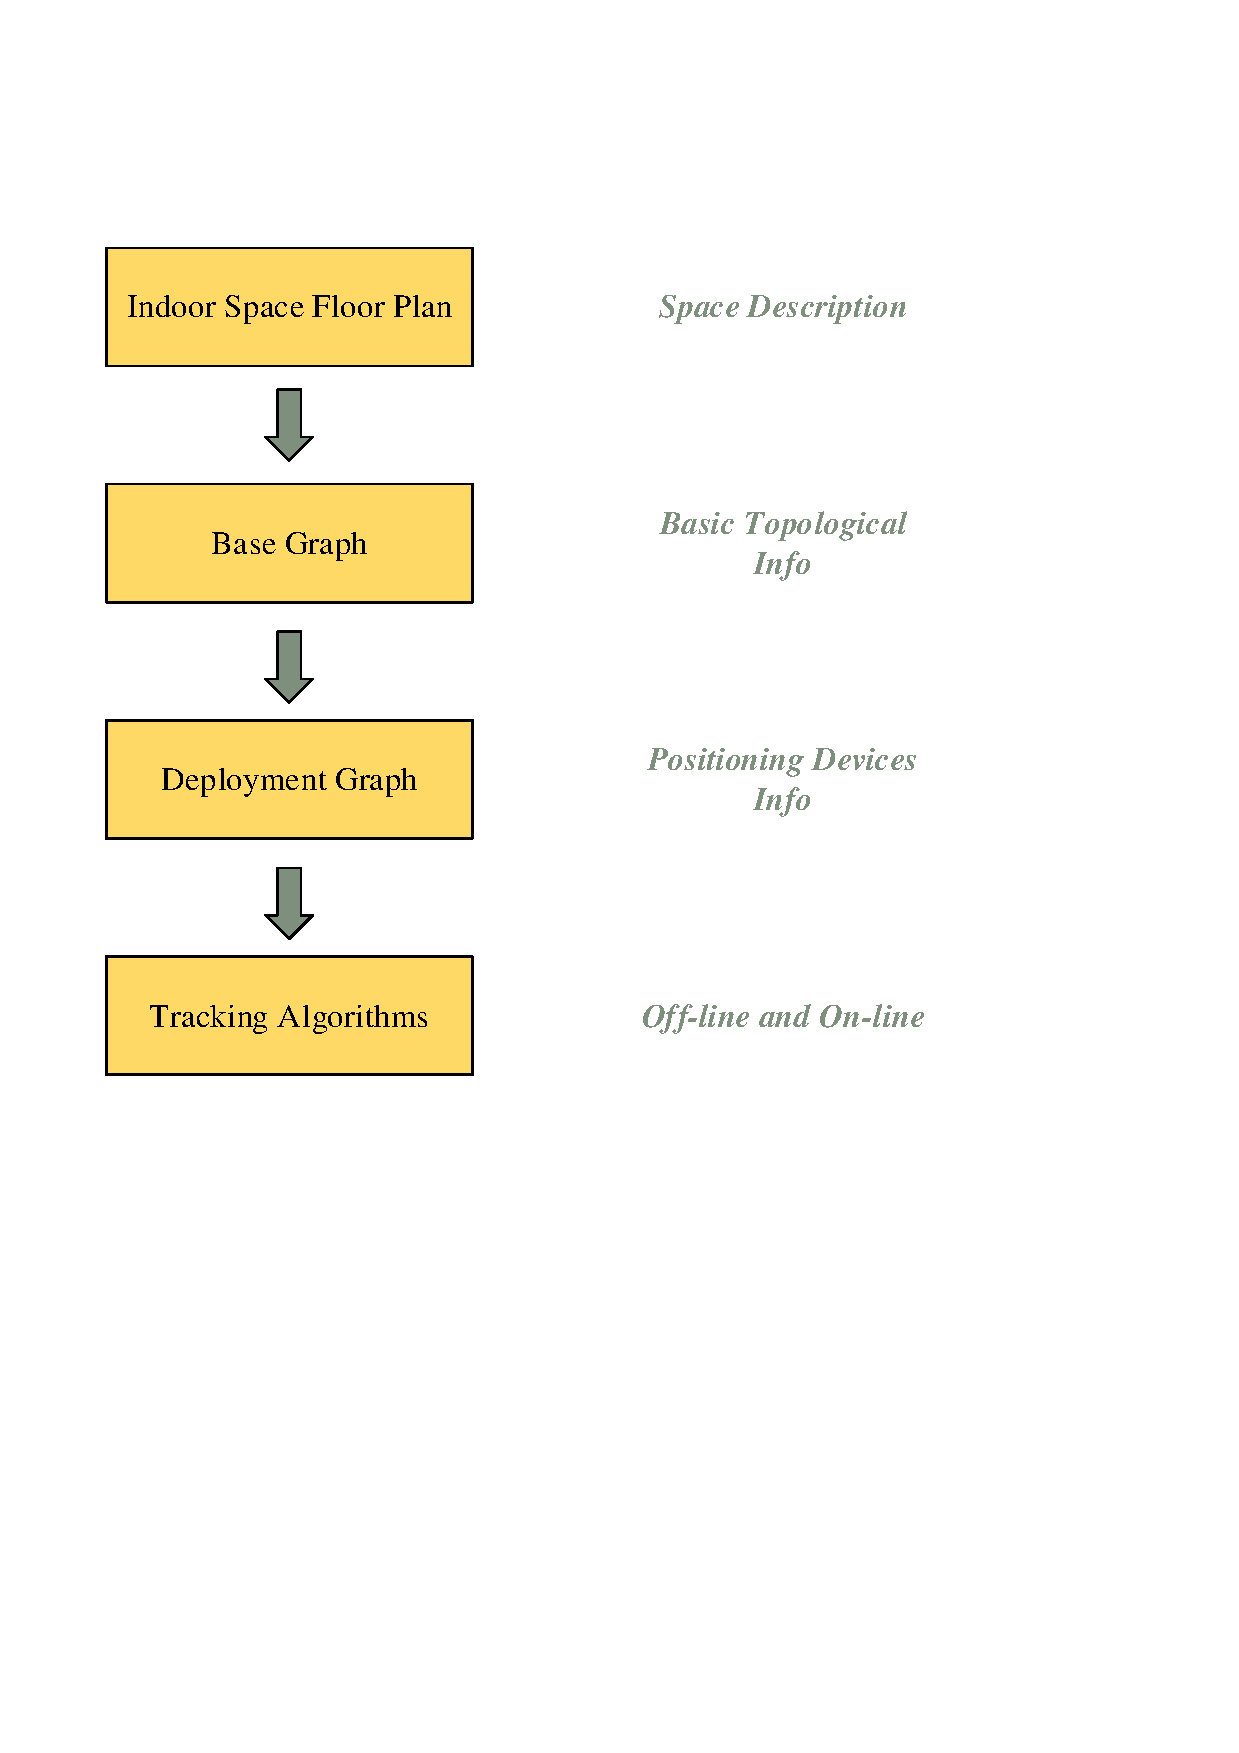
\includegraphics[width=\columnwidth]{figures/2-1/2-1-1.pdf}
    \end{figure}

  \column{.4\textwidth}
    \pause
    \conceptbf{Goal:} \textrm{Improve indoor tracking accuracy from a data management perspective, to capture where a particular object can be at a particular time.}

\end{columns}

\end{frame}

%------------------------------------------------

\begin{frame}
\frametitle{Base Graph Model}

\small{By capturing the essential connectivity and accessibility, \conceptbf{Base Graph} describes the topology of a floor plan of a possibly complex indoor space.}

\begin{columns}[c]

  \column{.45\textwidth}
    \begin{figure}[tb]
      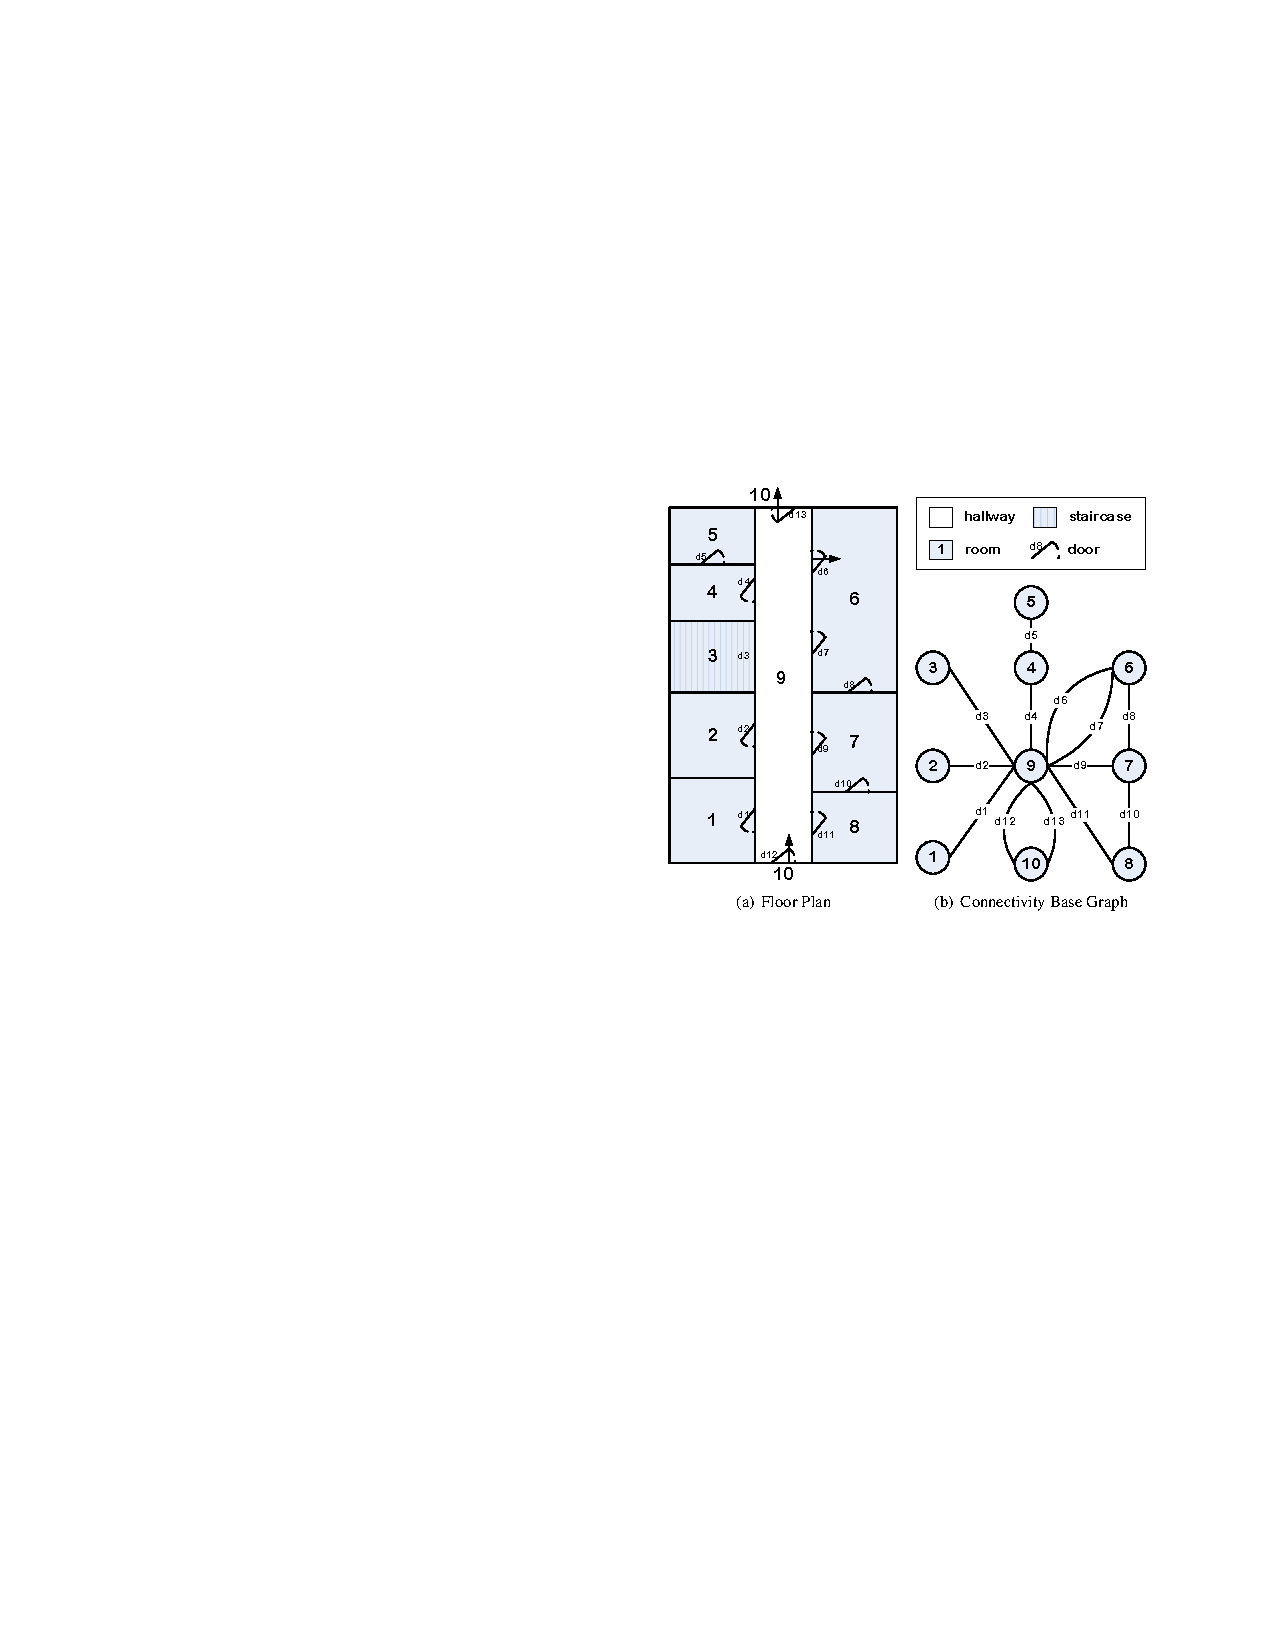
\includegraphics[width=\columnwidth]{figures/2-1/2-1-2.pdf}
    \end{figure}

  \column{.55\textwidth}
    \begin{block}{Connectivity Base Graph}
    a labeled, undirected graph.
      \textrm{
      \begin{itemize}
        \item $\mn{G_{conn} = \{V, E_d, \Sigma_{door}\}}$
        \item $\mn{V}$: each separate partition is represented as a vertex
        \item $\mn{E_d}$: each door is captured as an edge%, i.e., $\mn{(\{v_i,v_j}, k)}$
        \item $\mn{\Sigma_{door}}$: a set of edge labels that represent connections
      \end{itemize}
      }
    \end{block}

\end{columns}
\end{frame}

%------------------------------------------------

\begin{frame}
\frametitle{Base Graph Model}

  \small{\conceptbf{Accessibility Graph} is constructed to represent the movement permitted by doors or connections.}

\begin{columns}[c]

  \column{.45\textwidth}
    \begin{figure}[tb]
      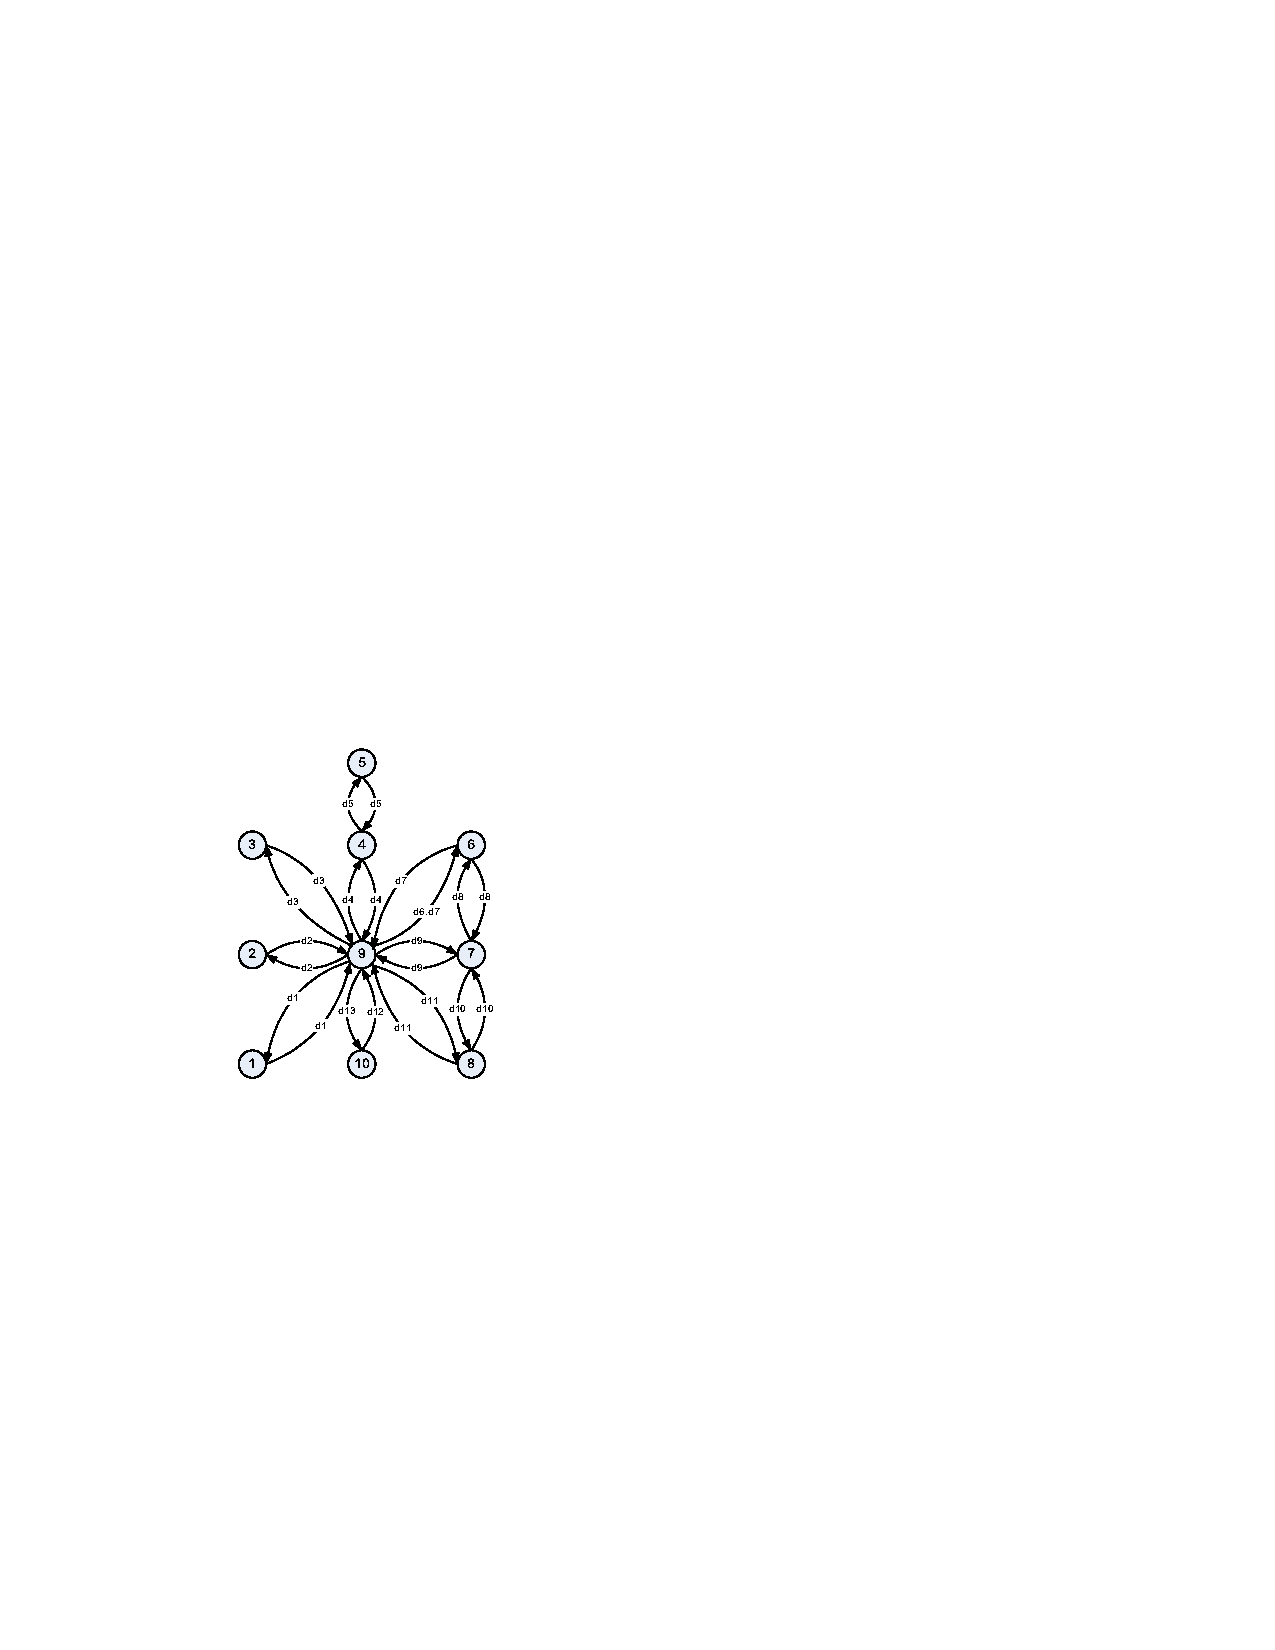
\includegraphics[width=\columnwidth]{figures/2-1/2-1-3.pdf}
    \end{figure}

  \column{.55\textwidth}
    \begin{block}{Accessibility Graph}
    a labeled, directed graph.
      \textrm{
      \begin{itemize}
        \item $\mn{G_{accs} = \{V, E, \Sigma_{door}, l_e\}}$
        \item $\mn{V}$: the set of vertices
        \item $\mn{E}$: the set of directed edges, i.e., $\mn{E=\{\langle v_i, v_j\rangle | v_i, v_j \in V \wedge v_i \neq v_j\}}$
        \item $\mn{l_e}$: a function that maps edges to subsets of the set of doors, i.e., $\mn{l_e : E \rightarrow 2^{\Sigma_{door}}}$
      \end{itemize}
      }
    \end{block}

\end{columns}
\end{frame}

%------------------------------------------------

\begin{frame}
\frametitle{Base Graph Model}

  \small{In addition to the topological information of a floor plan, its geometrical information should also be captured.}
  \\~\\
  \pause

  The \textrm{\em Building Partitions Mapping} is defined as:
  \pause
  \begin{equation}
  \mn{BuildingPartitions: V \rightarrow Ploygons}
  \end{equation}
  \\~\\
  \pause

  The \textrm{\em Doors Mapping} is defined as:
  \pause
  \begin{equation}
  \mn{Doors: \Sigma_{door} \rightarrow Line~Segments}
  \end{equation}

\end{frame}

%------------------------------------------------


\begin{frame}
\frametitle{RFID Deployment Graph Model}

\begin{itemize}
  \item RFID based proximity analysis
      \begin{itemize}
        %\item a record is produced when a \emph{RFID tag} approaches a \emph{RFID reader}.
        \item RFID readers deployment may cover only part of the space, or it may be capable of only detecting some movements in the space.
        \item assume that all RFID readers have disjoint activation ranges.
      \end{itemize}
  \item Types of RFID readers
      \begin{itemize}
        \item \conceptbf{Partitioning Readers} partition the indoor space into cells in the sense that an object cannot move from one cell to another without being observed.
        \item \conceptbf{Presence Readers} simply observe the presence(and non-presence) of tags in their activation ranges.
      \end{itemize}
\end{itemize}

\end{frame}

%------------------------------------------------

\begin{frame}
\frametitle{RFID Deployment Graph Model}

\small{Vertices represent cells. A directed edge indicates that one can move from one cell to another without entering other cells, which is detected by a corresponding partitioning reader.}

\begin{columns}[c]

  \column{.45\textwidth}
    \begin{figure}[tb]
      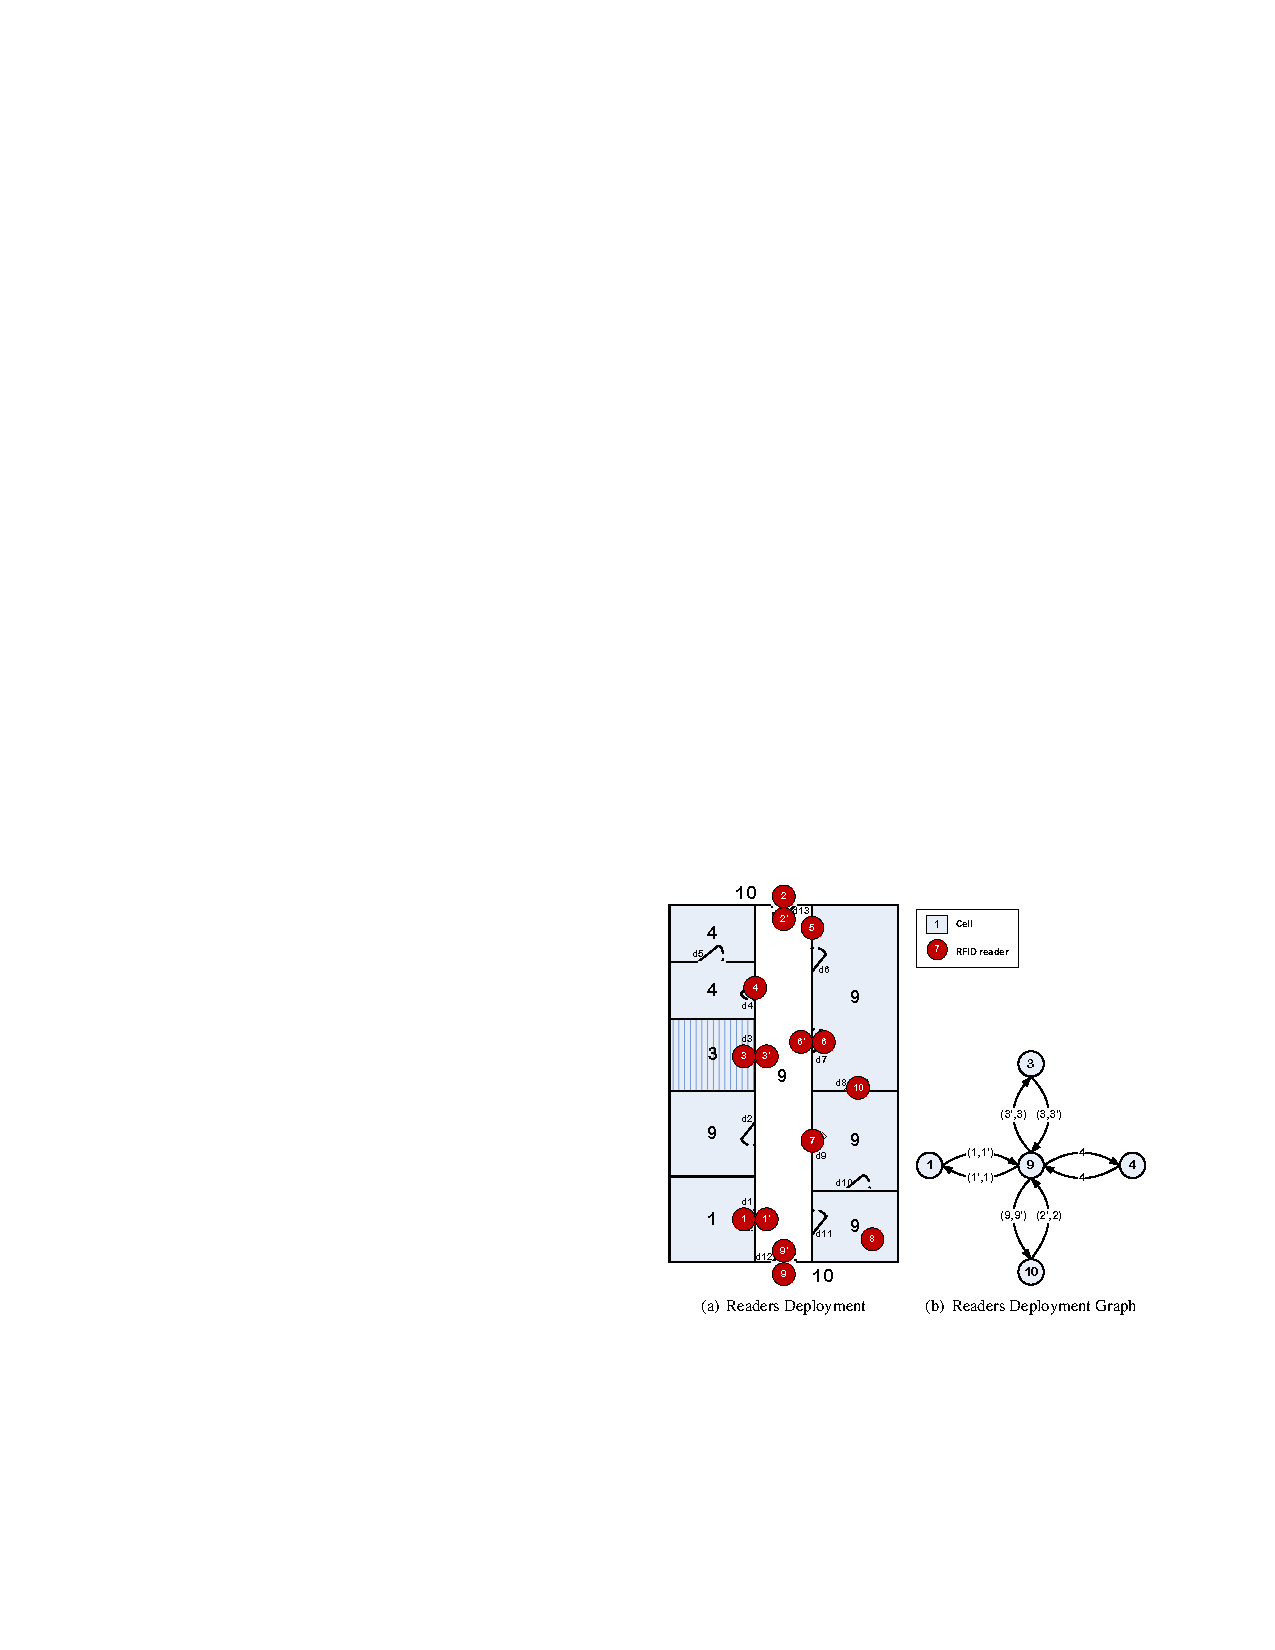
\includegraphics[width=\columnwidth]{figures/2-1/2-1-4.pdf}
    \end{figure}

  \column{.55\textwidth}
    \begin{block}{RFID Deployment Graph}
    a labeled, directed graph.
      \textrm{
      \begin{itemize}
        \item $\mn{G_{RFID} = \{C, E_r, \Sigma_{reader}, l_e\}}$
        \item $\mn{C}$: the set of the vertices
        \item $\mn{E_r}$: An edge is an ordered pair $\mn{\langle c_i, c_j \rangle}$ of distinct vertices from $\mn{C}$
        \item $\mn{l_e}$ maps an edge to a partitioning reader (pair), i.e., $\mn{E_r \rightarrow 2^{\Sigma_{reader}} \cup 2^{\Sigma_{reader} \times \Sigma_{reader}}}$
      \end{itemize}
      }
    \end{block}

\end{columns}
\end{frame}

%------------------------------------------------

\begin{frame}
\frametitle{RFID Deployment Graph Construction}

  \small{Each cell created by partitioning readers corresponds to one or more base graph partitions.}
  \pause
  \begin{equation}
  \mn{Cells: V \rightarrow C}
  \end{equation}
  \\~\\
  \pause

  \small{For each RFID reader, record its accurate deployment location and activation range.}
  \pause
  \begin{equation}
  \begin{split}
  \mn{Mapping~1}: & \mn{\Sigma_{reader} \rightarrow \{ (loc, range, flag)~|~loc \in R^2 \wedge} \\
    & \mn{range \in (0,d_{max}] \wedge flag \in \{ PAR, PRE \} \}}
  \end{split}
  \end{equation}
  \\~\\
  \pause

  \small{A mapping of readers to the cells that their activation ranges intersect is introduced as:}
  \pause
  \begin{equation}
  \mn{
  Mapping~2: \Sigma_{reader} \rightarrow 2^C
  }
  \end{equation}

\end{frame}

%------------------------------------------------

\begin{frame}
\frametitle{RFID Deployment Graph Construction}

\begin{columns}[c]

  \column{.47\textwidth}
    \begin{figure}[tb]
      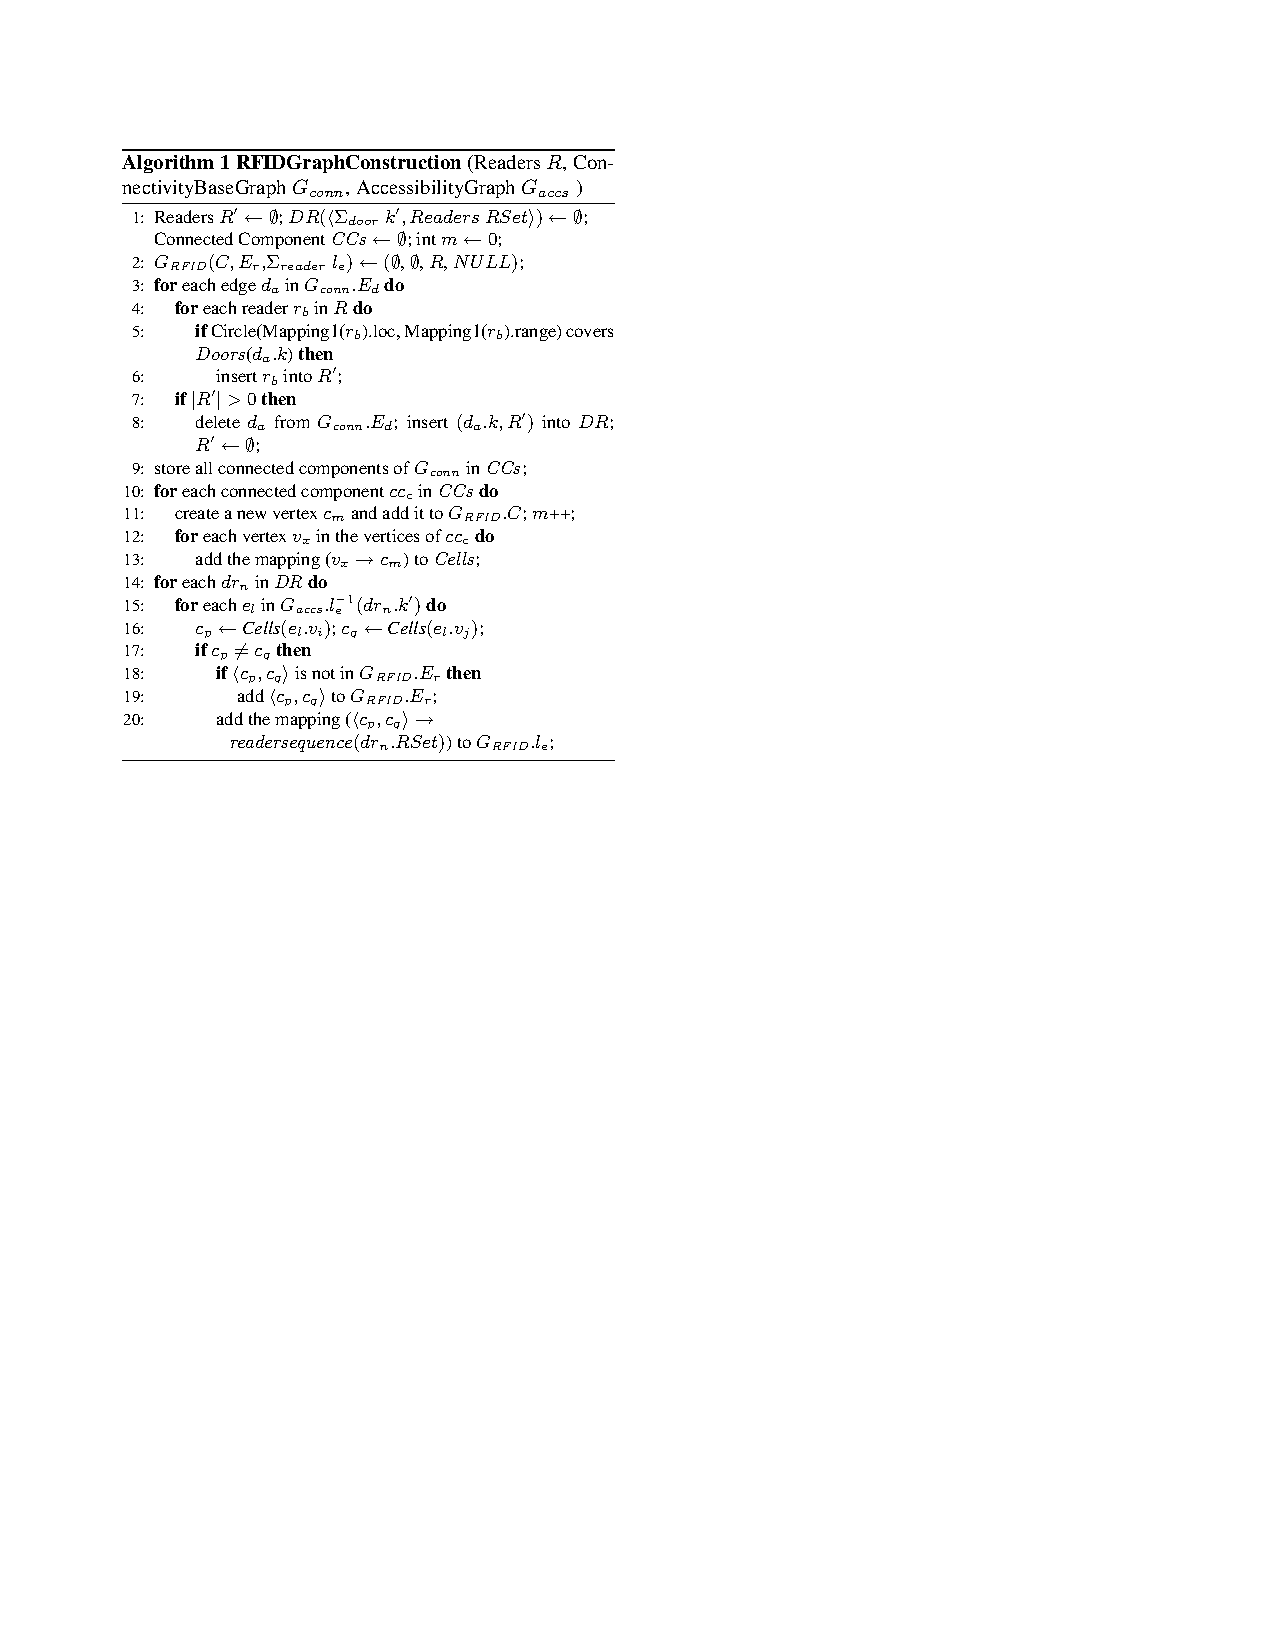
\includegraphics[width=\columnwidth]{figures/2-1/2-1-5.pdf}
    \end{figure}

  \column{.53\textwidth}
  \ssize{
    \begin{enumerate}
      \pause
      \item Input: \textrm{the reader set $\mn{R}$, the connectivity base graph $\mn{G_{conn}}$, the accessibility graph $\mn{G_{accs}}$} \pause
      \item Lines 1--2: \textrm{Initialize $\mn{G_{RFID}}$, $\mn{DR}$, $\mn{CCs}$} \pause
      \item Lines 3--8: \textrm{the relationship of which door is covered by which readers is captured in $\mn{DR}$} \pause
      \item Lines 9--13: \textrm{a deployment graph vertex is created for each $\mn{CC}$, mapping $\mn{Cells}$ is also stored} \pause
      \item Lines 14--20: \textrm{for each door in $\mn{DR}$, determine if its edges' head and tail are mapped to different cells. If so, add an edge to deployment graph. Function $\mn{readersequence}$ returns the possible reader sequence for that edge}
    \end{enumerate}
  }
  \end{columns}

\end{frame}

%------------------------------------------------

\begin{frame}
\frametitle{RFID-based Indoor Tracking}

  \small{\conceptbf{Raw Trajectories}: \textrm{Sequences of RFID Tag Observation}}

  \begin{columns}[c]

  \column{.47\textwidth}
    \begin{figure}[tb]
      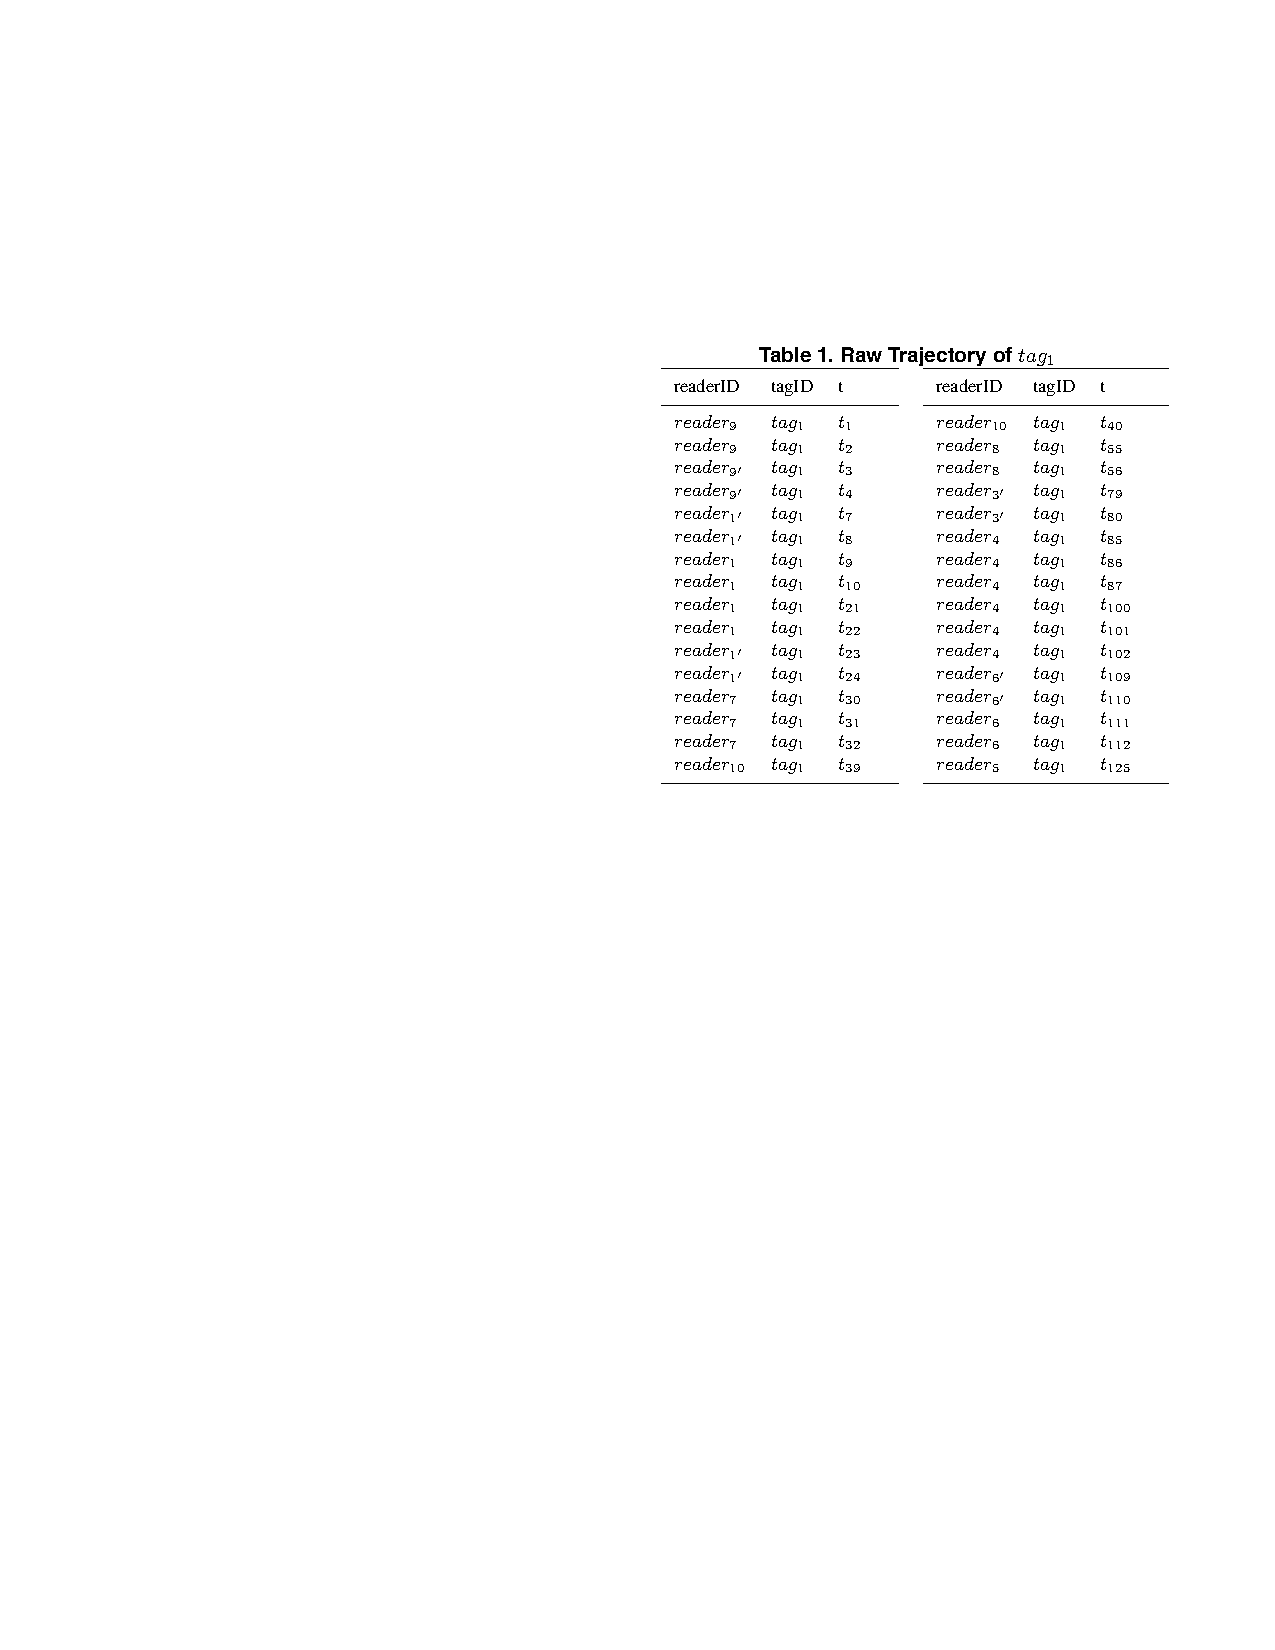
\includegraphics[width=\columnwidth]{figures/2-1/2-1-6.pdf}
    \end{figure}
    \ssize{\textit{
      1. each reader detects and reports tags with a sampling rate \\
      2. formatted as $\mn{\langle readerID, tagID, t \rangle}$
    }}

  \column{.53\textwidth}
    \begin{figure}[tb]
      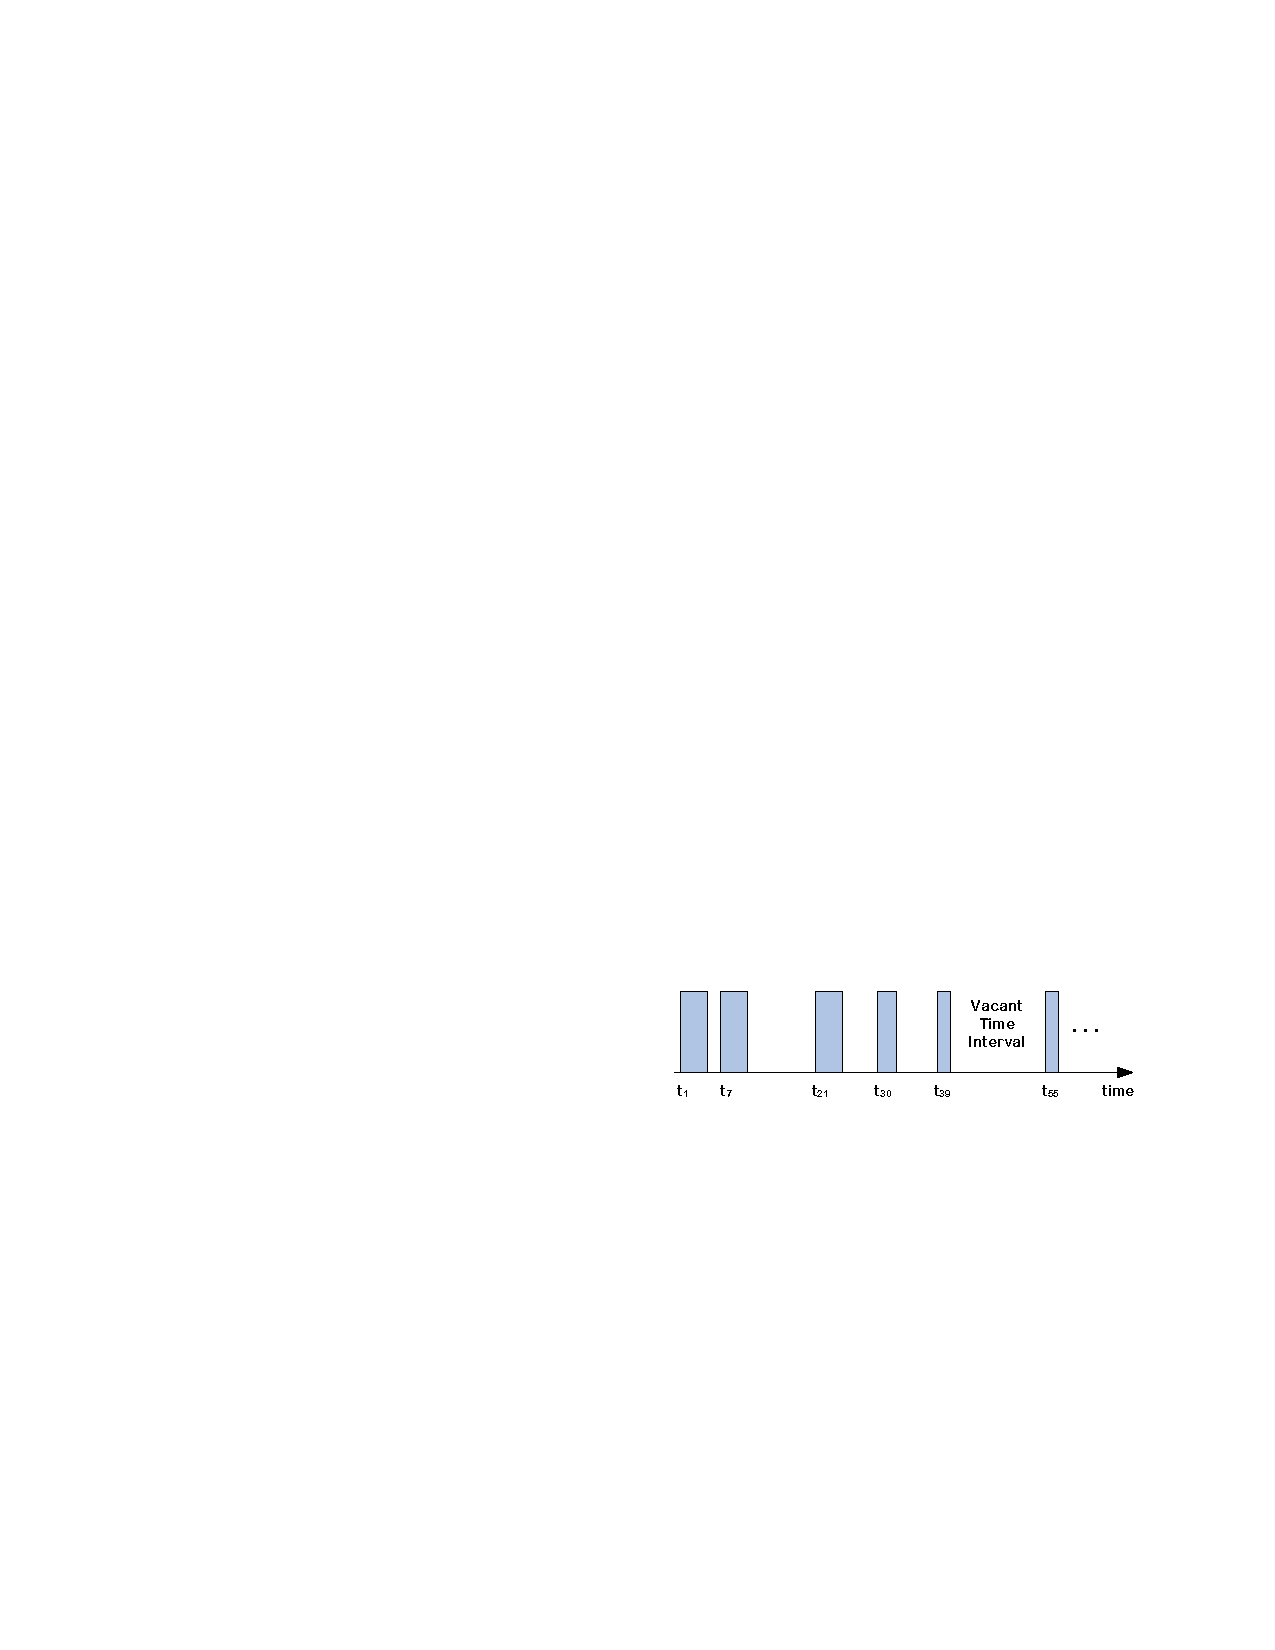
\includegraphics[width=\columnwidth]{figures/2-1/2-1-7.pdf}
    \end{figure}

    \vspace{-15pt}
    \ssize{
      \begin{itemize}
        \pause
        \item \emph{vacant time intervals}: unable to observe the moving objects \pause
        \item to search RFID deployment graph to infer the possible regions of moving object \pause
        \item to apply maximum speed position interpolation to further shrink the possible regions~\cite{civilis2005techniques, pfoser1999capturing}
      \end{itemize}
    }

  \end{columns}

\end{frame}

%------------------------------------------------

\begin{frame}
\frametitle{RFID Readings Pre-processing}

  \small{Step-1's output is used in on-line tracking, while Step-2's is used in off-line tracking}

  \begin{columns}[c]

  \column{.47\textwidth}
    \begin{figure}[tb]
      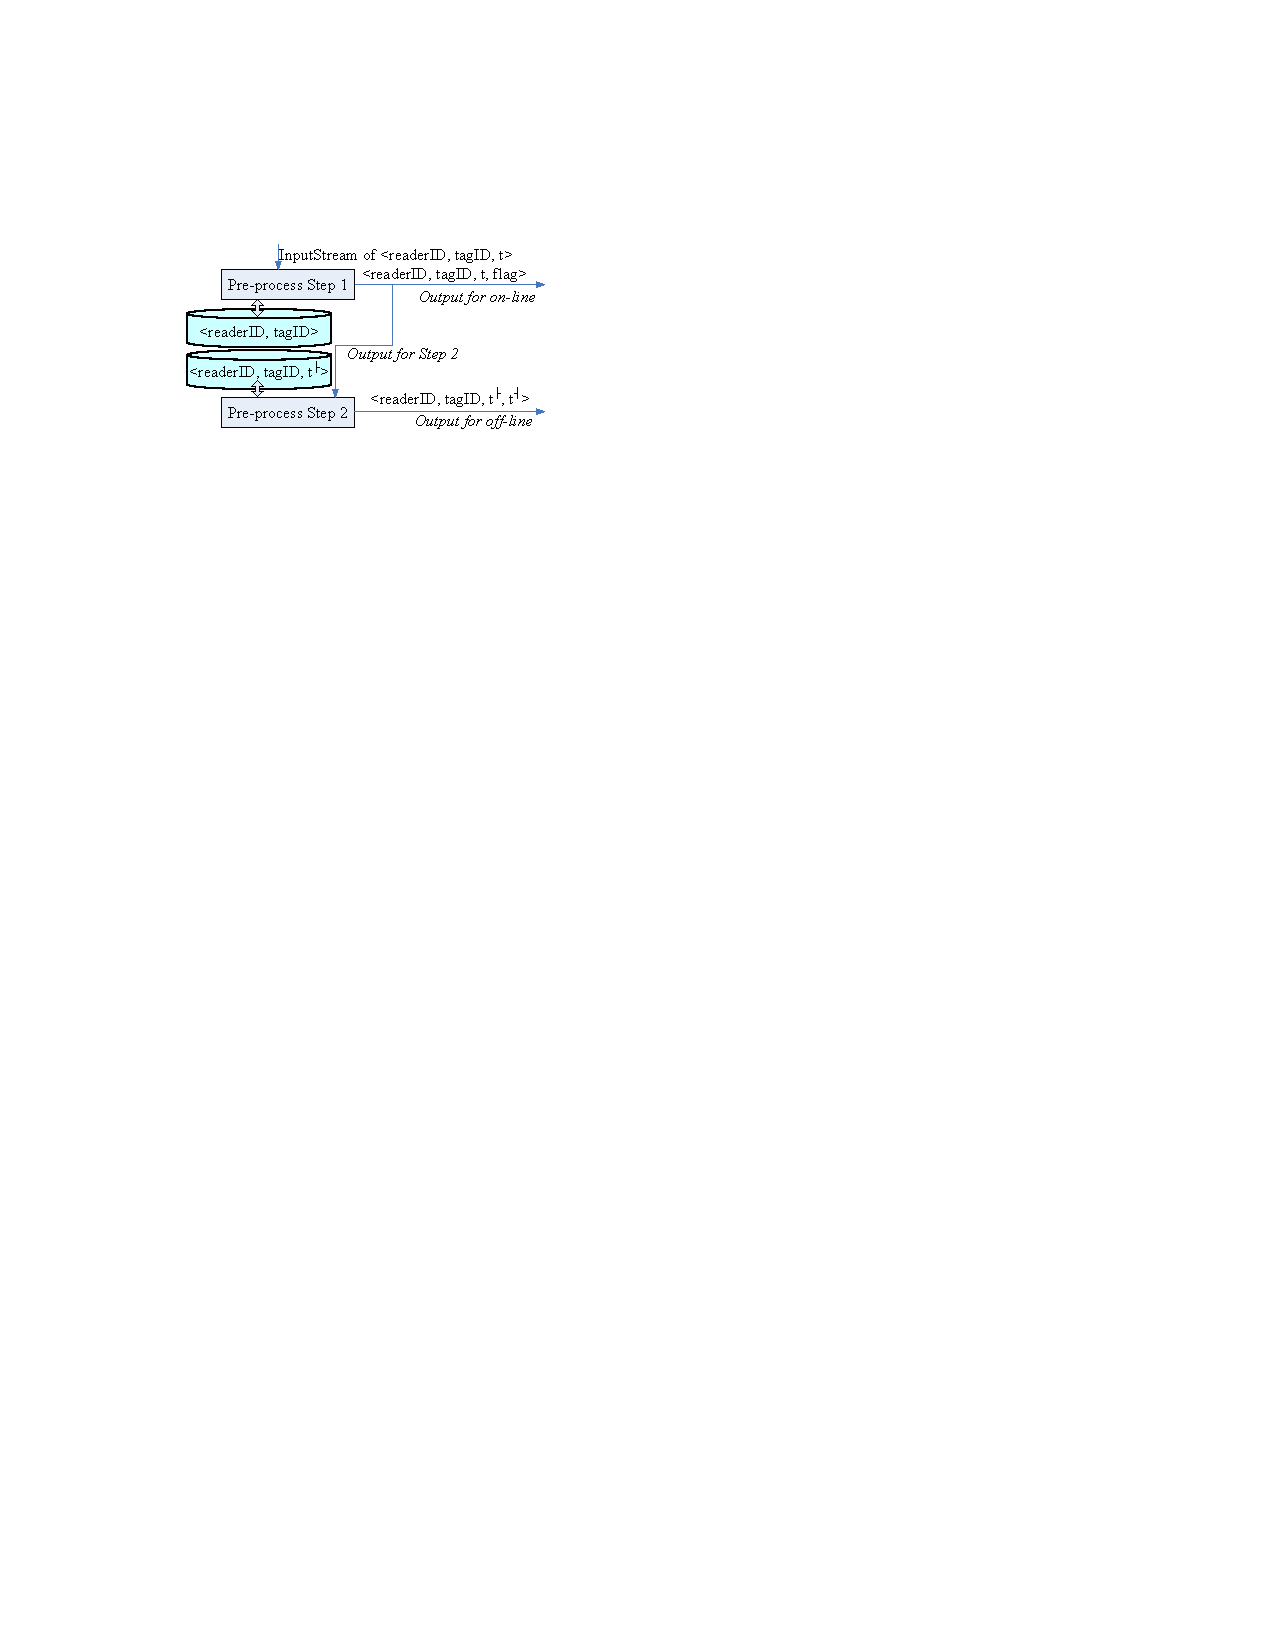
\includegraphics[width=\columnwidth]{figures/2-1/2-1-8.pdf}
    \end{figure}

  \column{.53\textwidth}
    \begin{itemize}
        \item $\mn{Flag \in \{ START, END \}}$
        \item $\mn{START} \rightarrow$ \textrm{enters the range}
        \item $\mn{END} \rightarrow$ \textrm{leaves the range}
    \end{itemize}

  \end{columns}

\end{frame}

%------------------------------------------------

\begin{frame}
\frametitle{Off-line Tracking (Refinement Step 1)}

  \begin{columns}[c]

  \column{.43\textwidth}
    \vspace{-15pt}
    \begin{figure}[tb]
      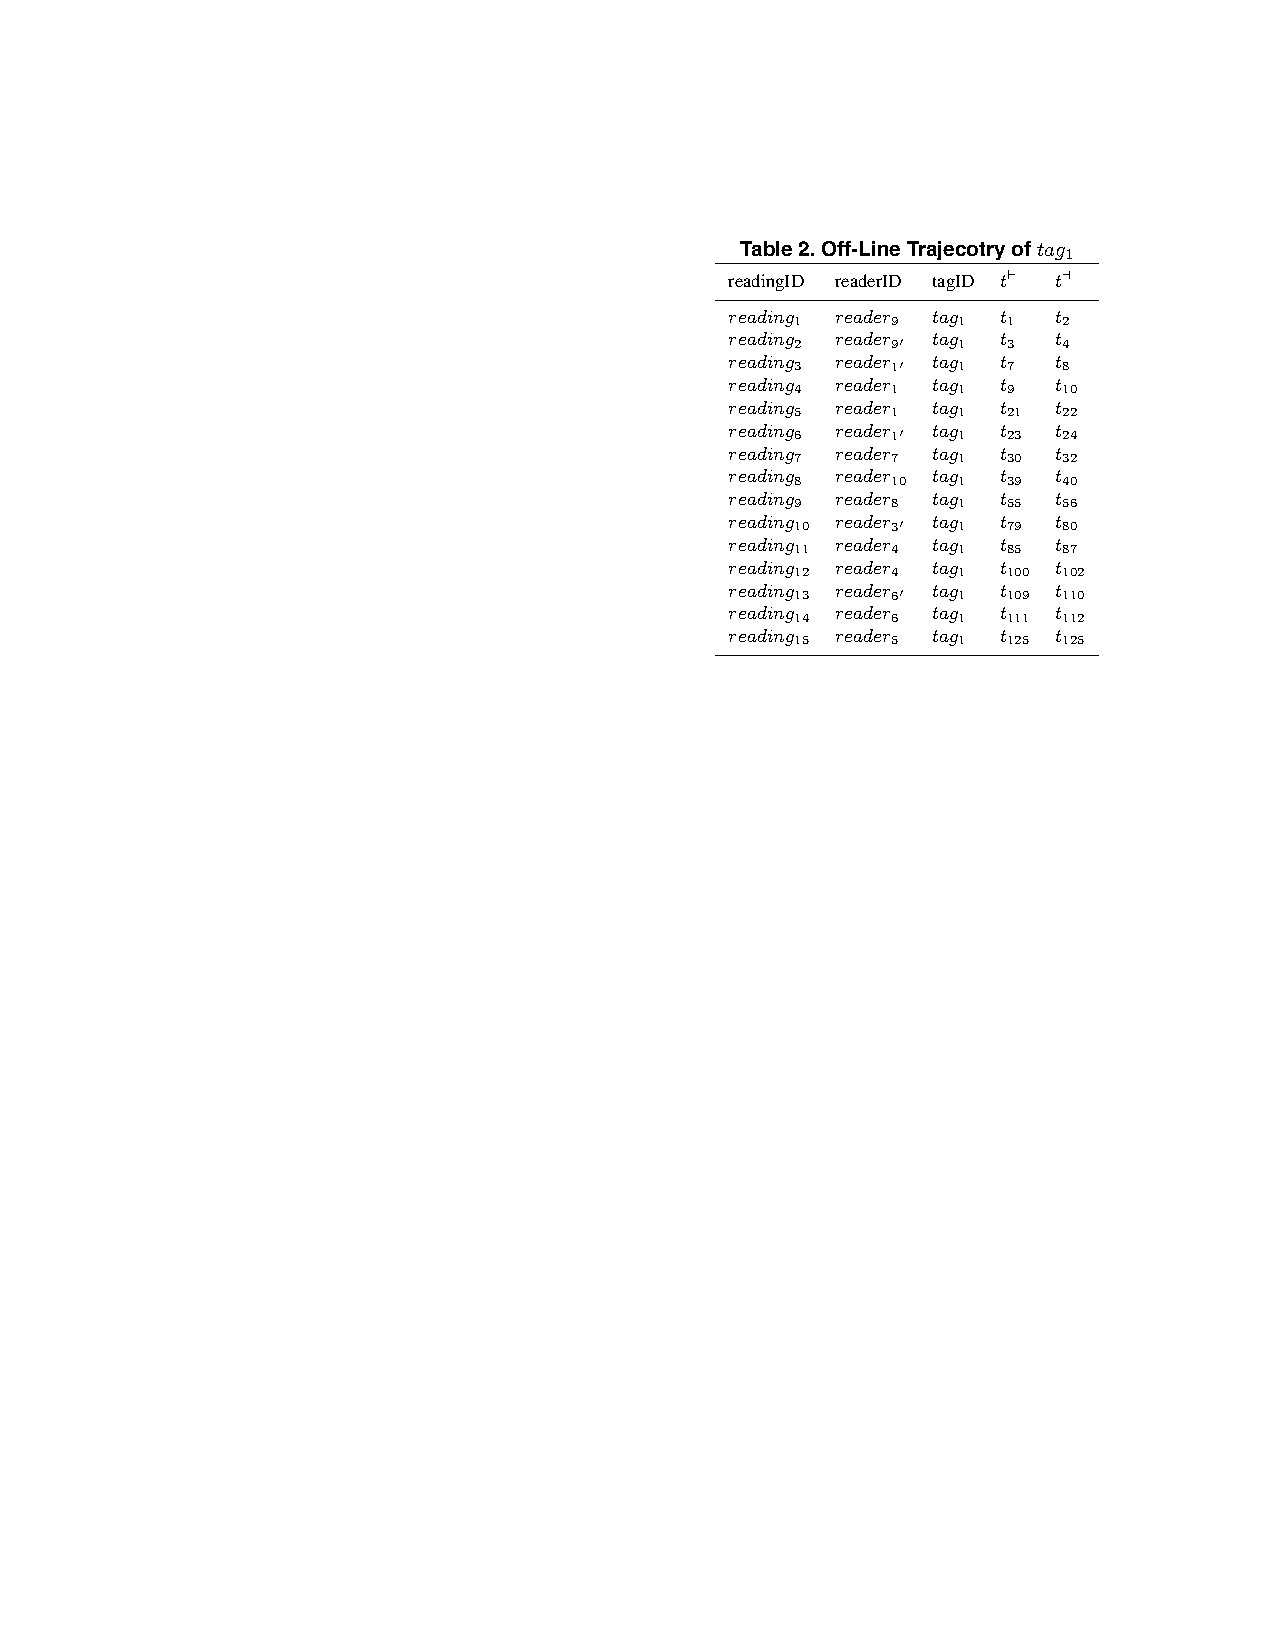
\includegraphics[width=0.92\columnwidth]{figures/2-1/2-1-9.pdf}
    \end{figure}
    \vspace{-20pt}
    \begin{figure}[tb]
      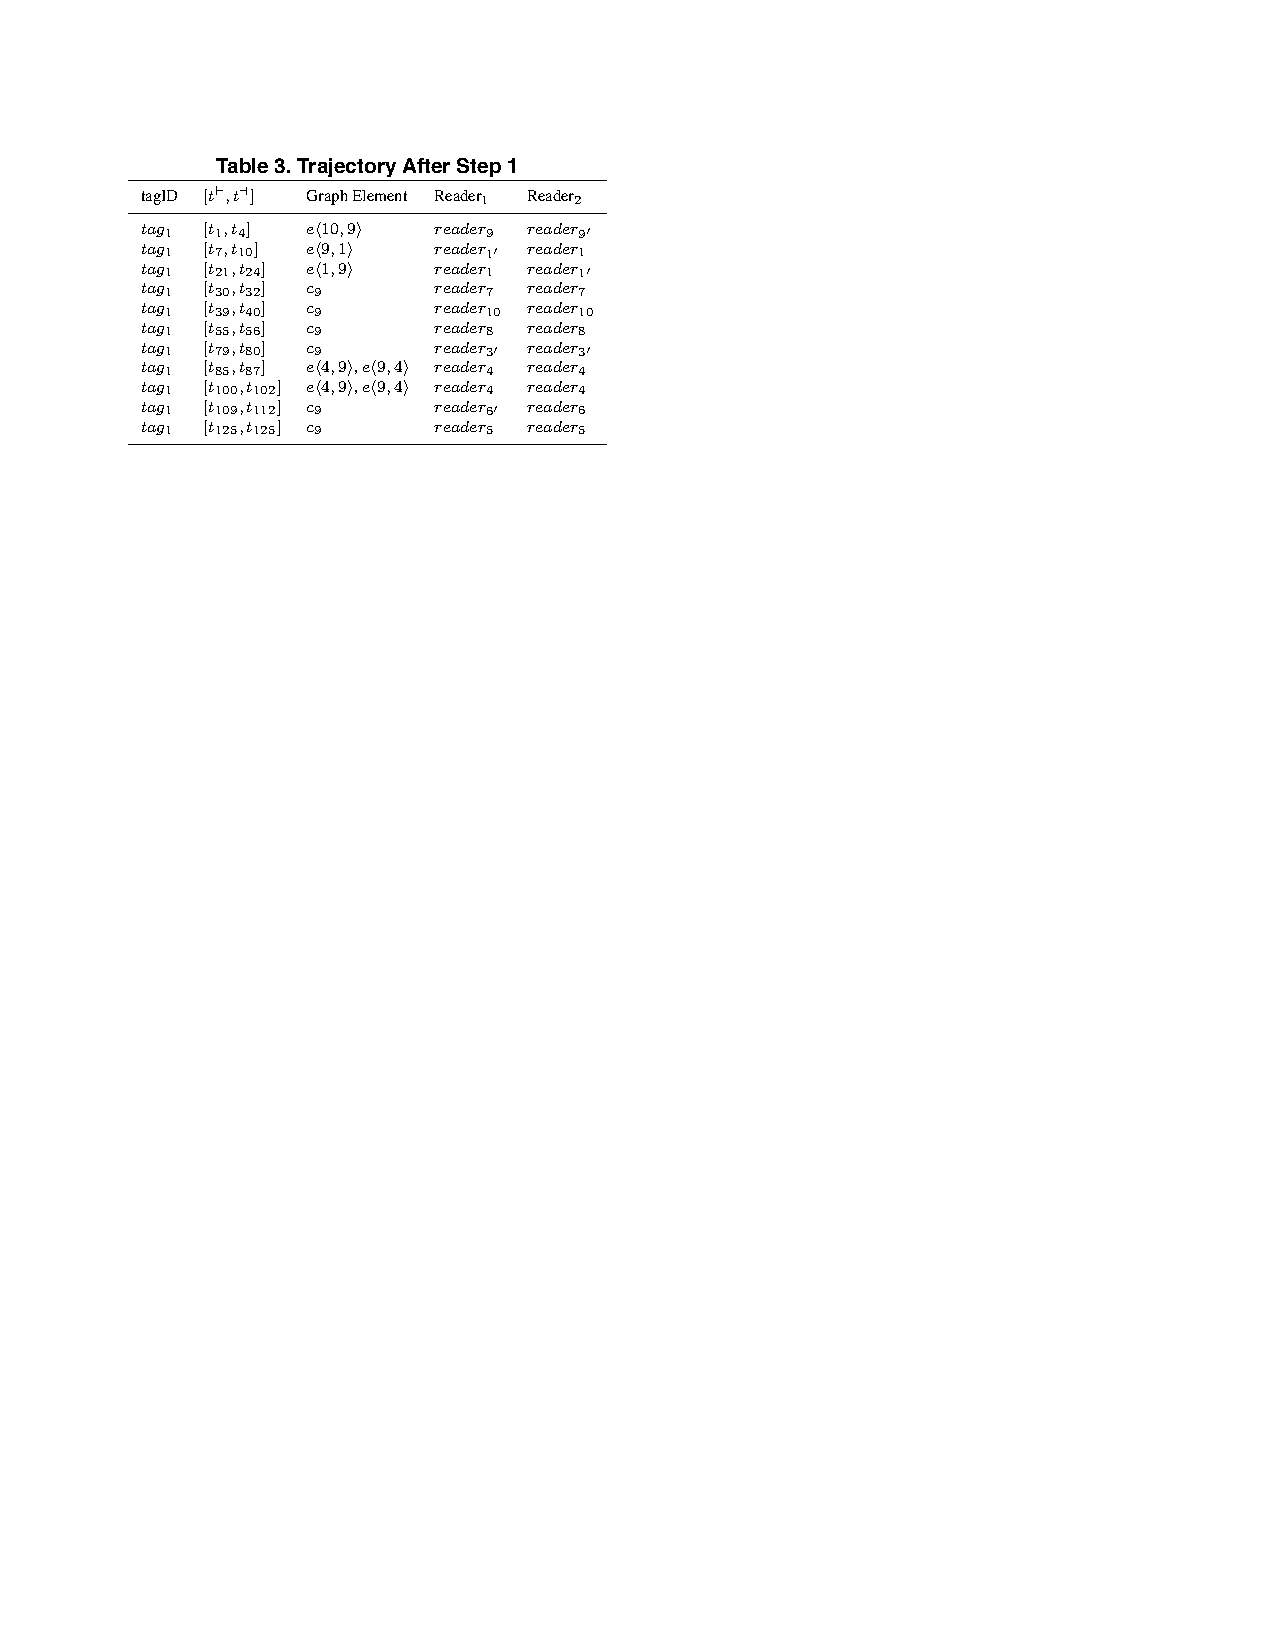
\includegraphics[width=\columnwidth]{figures/2-1/2-1-10.pdf}
    \end{figure}


  \column{.57\textwidth}
  \fsize{
    \begin{itemize}
      \item Step 1 transforms an RFID reading sequence to corresponding vertices or edges in deployment graph
      \item If two consecutive reading sequences are \emph{contiguous}, they should stem from a partitioning pair, which map to an edge
      \item Otherwise, should come from either a single $\mn{PRE}$ or a $\mn{PAR}$ reader
      \item A $\mn{PAR}$ is replaced by the set of corresponding edges according to $\mn{G_{RFID}.{l_e}^{-1}}$
      \item A $\mn{PRE}$ always corresponds to one or several cells according to $\mn{Mapping~2}$
    \end{itemize}
  }
  \end{columns}

\end{frame}

%------------------------------------------------

\begin{frame}
\frametitle{Off-line Tracking (Refinement Step 2)}

\begin{columns}[c]

  \column{.43\textwidth}
  \vspace{-15pt}
  \begin{figure}[tb]
    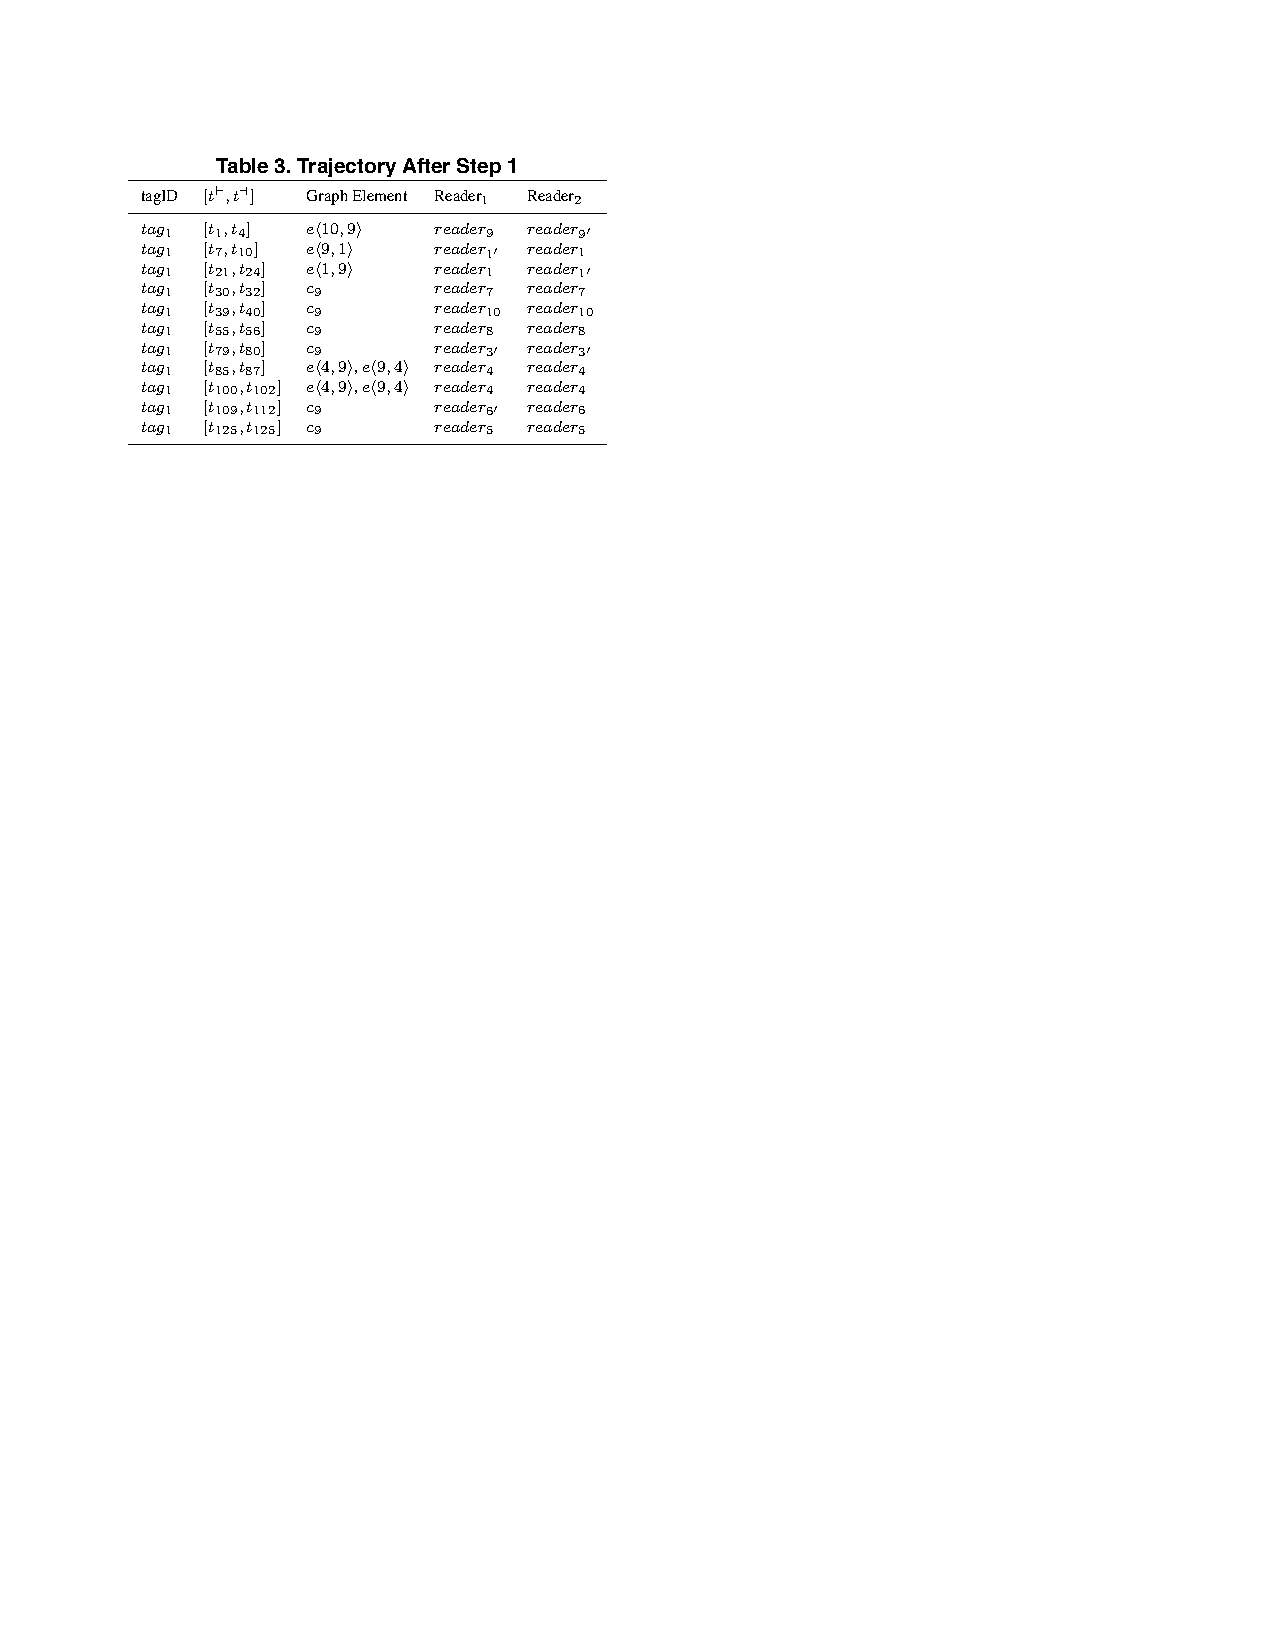
\includegraphics[width=\columnwidth]{figures/2-1/2-1-10.pdf}
  \end{figure}
  \vspace{-20pt}
  \begin{figure}[tb]
    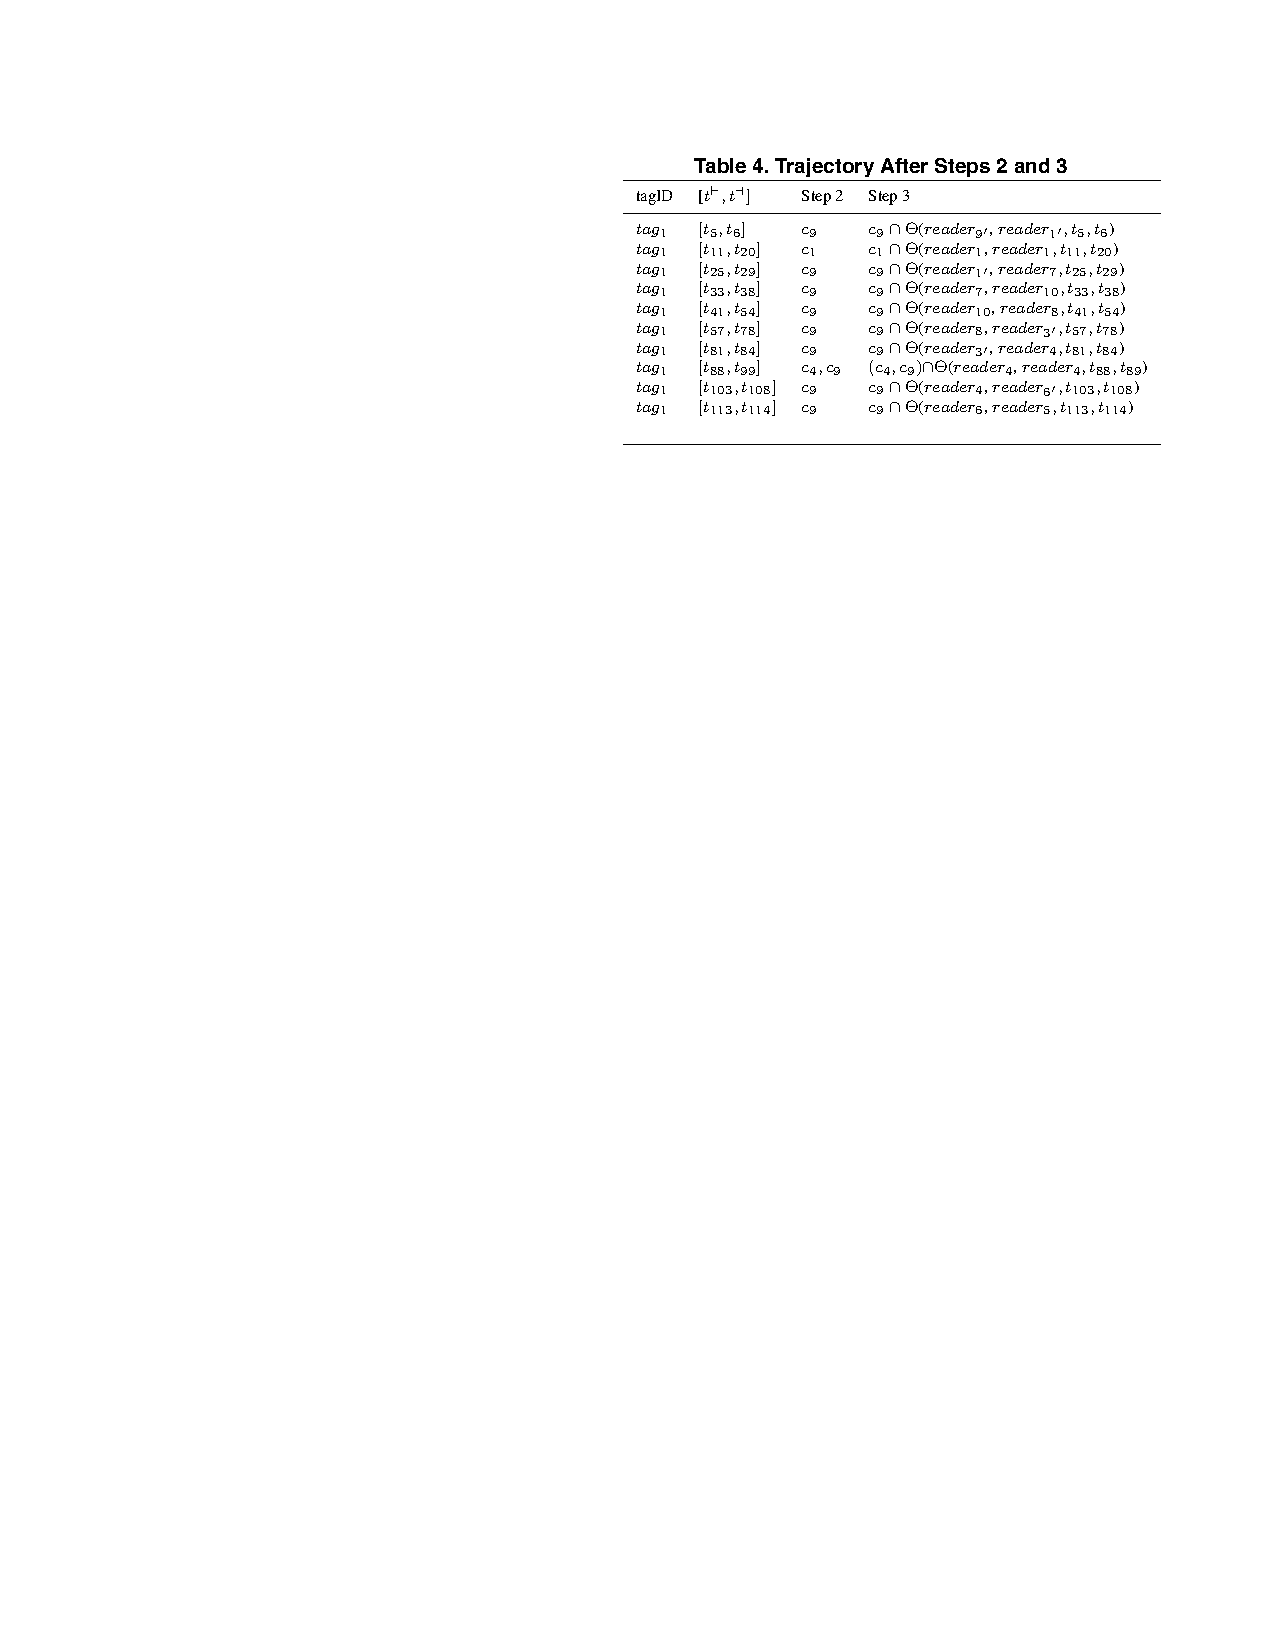
\includegraphics[width=\columnwidth]{figures/2-1/2-1-11.pdf}
  \end{figure}


  \column{.57\textwidth}
  \fsize{
    \begin{itemize}
      \item The \emph{graph elements} from Step 1 indicates some region(s) within which the object may be in during the vacant time interval
      \item Check its previous record's tail element and current record's head element, select their intersection as Step 2's candidate
    \end{itemize}
  }

\end{columns}

\end{frame}

%------------------------------------------------

\begin{frame}
\frametitle{Off-line Tracking (Refinement Step 3)}

\begin{columns}[c]

\column{.48\textwidth}
\begin{itemize}
\ssize{
  \item Calculate the \emph{possible region} $\mn{\Theta}$ according to maximum speed limit

  \item Circle based possible region
    \begin{itemize}
      \tiny{
        \item locations: $\mn{P_{9'}}$, $\mn{P_{1'}}$
        \item activation ranges: $\mn{R_{9'}}$, $\mn{R_{1'}}$
        \item for $\mn{t_x \in [ t_5, t_6 ]}$, $\mn{\Delta t_1 = t_x - reading_2.t^{\vdash}}$, $\mn{\Delta t_2 = reading_3.t^{\dashv} - t_x}$
        \item $\mn{R_3 = R_{9'} + V_{max} * \Delta t_1}$, $\mn{R_5 = R_{1'} + V_{max} * \Delta t_2}$
      }
    \end{itemize}

  \item Ellipse based possible region
  \begin{itemize}
      \tiny{
        \item foci: two points belonging to the circle centered at $\mn{P_{9'}}$, $\mn{P_{1'}}$
        \item length of major axis is:
          \begin{equation*}
            \mn{2a = V_{max} * (\Delta t_1 + \Delta t_2)}
          \end{equation*}
      }
  \end{itemize}
}
\end{itemize}

\column{.52\textwidth}
\vspace{-15pt}
\begin{figure}[tb]
  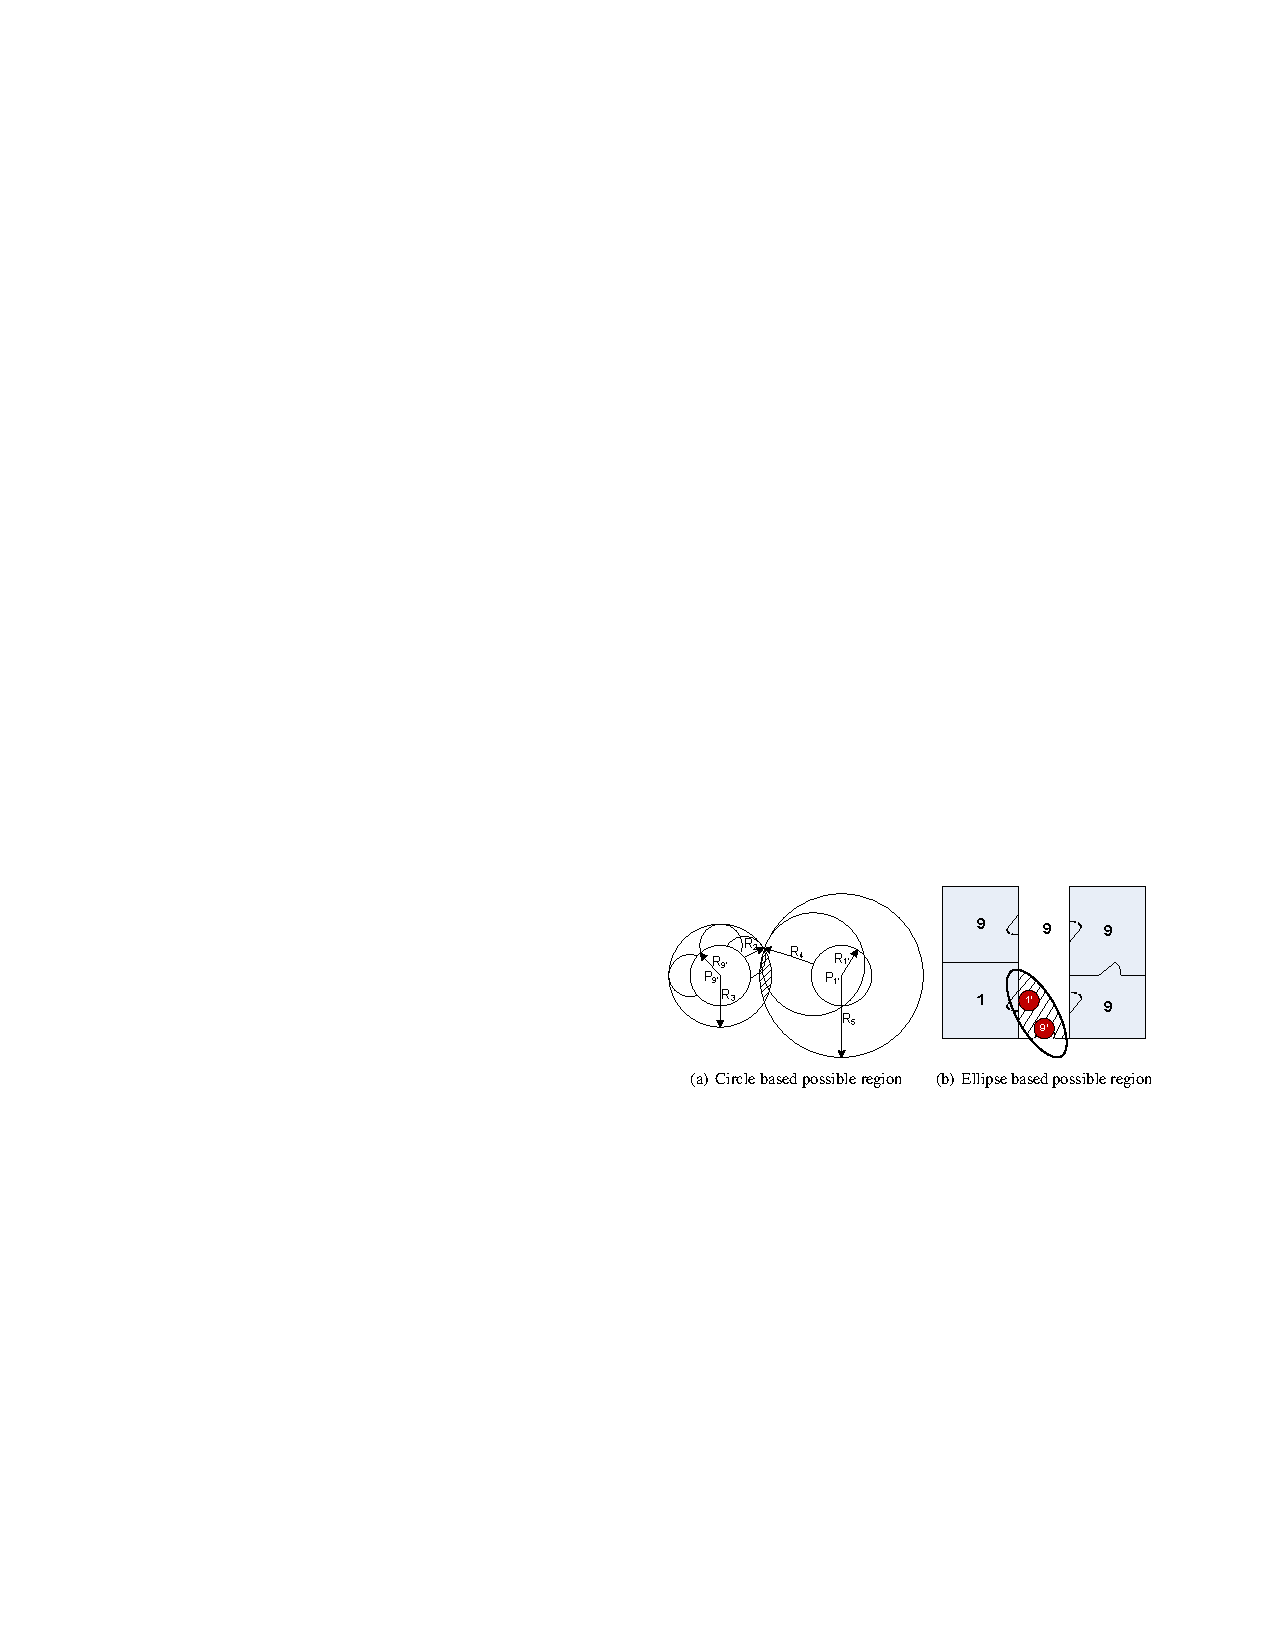
\includegraphics[width=\columnwidth]{figures/2-1/2-1-12.pdf}
\end{figure}
\tiny{
  \pause
  $\left.\begin{matrix}
  \mn{(reading_1, reader_{9}, tag_1, t_1, t_2)}~~\\
  \mn{(reading_2, reader_{9'}, tag_1, t_3, t_4)}~~\\
  \mn{(reading_3, reader_{1'}, tag_1, t_7, t_8)}~~\\
  \mn{(reading_4, reader_{1}, tag_1, t_9, t_10)}~~
  \end{matrix}\right\} \overset{Step~1}{\rightarrow} \pause$ \\~\\~\\

  $\left.\begin{matrix}
  \mn{(tag_1, [t_1,t_4], e\langle 10,9 \rangle, reader_{9}, reader_{9'})}~~\\
  \mn{(tag_1, [t_7,t_{10}], e\langle 9,1 \rangle, reader_{1'}, reader_{1})}~~
  \end{matrix}\right\} \overset{Step~2}{\rightarrow} \pause$ \\~\\~\\

  $\mn{(tag_1, [t_5,t_6], c_9, reader_{9'}, reader_{1'})} \overset{Step~3}{\rightarrow} \pause$ \\~\\~\\

  $\mn{(tag_1, [t_5,t_6], c_9 \cup \Theta(reader_{9'}, reader_{1'}, t_5, t_6))}$
}

\end{columns}

\end{frame}

%------------------------------------------------

\begin{frame}
\frametitle{On-line Tracking}

\small{\textrm{Given $\mn{\langle readerID, tagID, t, flag \rangle}$. \conceptbf{On-line tracking} is intended to infer the trajectory in the time interval between the last observation and the current time or even in the future.}}
\\~\\

\begin{columns}[c]

  \column{.35\textwidth}
  \begin{figure}[tb]
    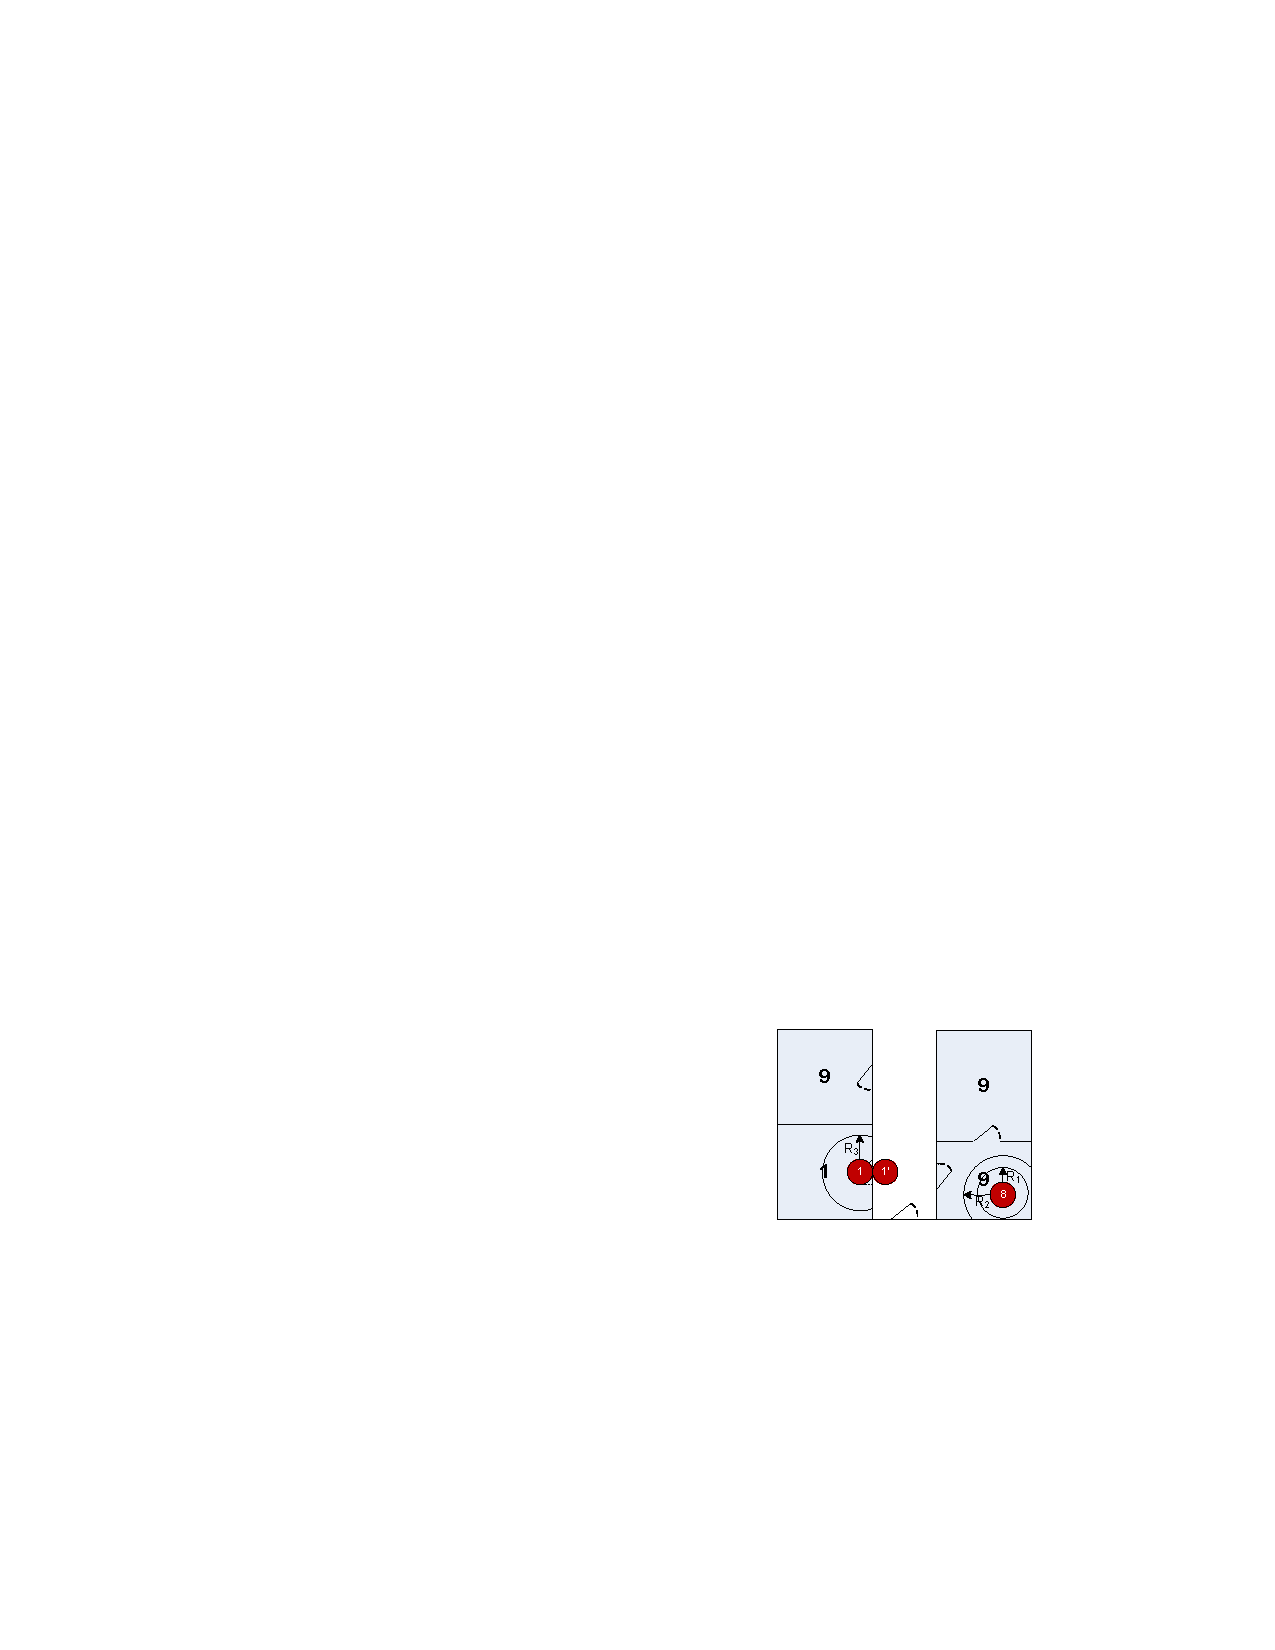
\includegraphics[width=\columnwidth]{figures/2-1/2-1-13.pdf}
  \end{figure}


  \column{.65\textwidth}
  \fsize{
    \begin{itemize}
      \item $\mn{flag = START}$, object $\mn{tagID}$ is in the activation range of $\mn{readerID}$ at time $\mn{t}$.
      \item $\mn{flag = END}$, the object is beyond the activation range of $\mn{readerID}$ and not in the range of any other readers.
				\begin{itemize}
					\ssize{
					\item constrains by a circle determined by the most recent observing reader's range.
					\item further refined if an object has recently been detected by a partitioning reader pair.
					}
				\end{itemize}
    \end{itemize}
  }

\end{columns}

\end{frame}

%------------------------------------------------

\begin{frame}
\frametitle{Research Directions}

\begin{itemize}
	\item Extend the deployment graphs to accommodate RFID readers with large and overlapping activation ranges. \\~\\
	\item Using multiple deployment graphs for several positioning technologies. \\~\\
	\item To enhance on-line tracking. Historical data $\rightarrow$ association rules $\rightarrow$ better prediction.
\end{itemize}

\end{frame}

% \begin{frame}[allowframebreaks]
\frametitle{References}

\begin{thebibliography}{99} % Beamer does not support BibTeX so references must be inserted manually as below
\fsize{

\bibitem{DBLP:conf/mdm/JensenLY09}
C.S.~Jensen, H.~Lu, B.~Yang.
\newblock Graph model based indoor tracking.
\newblock In {\em {MDM}}, pp. 122--131, 2009.

\bibitem{civilis2005techniques}
A.~Civilis, C.S.~Jensen, S.~Pakalnis.
\newblock Techniques for efficient road-network-based tracking of moving objects.
\newblock In {\em {TKDE}}, pp. 698--712, 2005.

\bibitem{pfoser1999capturing}
D.~Pfoser, C.S.~Jensen.
\newblock Capturing the uncertainty of moving-object representations.
\newblock In {\em {Advances in Spatial Databases}}, pp. 111--131, 1999.

}
\end{thebibliography}

\end{frame}


\subsection{2.2 Scalable Continuous Range Monitoring of Moving Objects in Symbolic Indoor Space} % A subsection can be created just before a set of slides with a common theme to further break down your presentation into chunks

% \begin{frame}
\frametitle{About This Work...}

\emph{Scalable Continuous Range Monitoring of Moving Objects in Symbolic Indoor Space}.~\cite{DBLP:conf/cikm/YangLJ09} \\
B.~Yang, H.~Lu, and C.~S. Jensen.\\~\\

\begin{itemize}
  \item Published in \emph{CIKM' 2009}.
\end{itemize}

\end{frame}

%------------------------------------------------

% \begin{frame}[allowframebreaks]
\frametitle{References}

\begin{thebibliography}{99} % Beamer does not support BibTeX so references must be inserted manually as below
\fsize{

\bibitem{DBLP:conf/mdm/JensenLY09}
C.~S. Jensen, H.~Lu, and B.~Yang.
\newblock Graph model based indoor tracking.
\newblock In {\em {MDM}}, pp. 122--131, 2009.

\bibitem{DBLP:conf/cikm/YangLJ09}
B.~Yang, H.~Lu, and C.~S. Jensen.
\newblock Scalable continuous range monitoring of moving objects in symbolic
  indoor space.
\newblock In {\em CIKM}, pp. 671--680, 2009.

\bibitem{becker2005location}
C.~Becker and F.~D{\"u}rr.
\newblock On location models for ubiquitous computing.
\newblock In {\em Personal and Ubiquitous Computing}, pp. 20--31, 2005.

\bibitem{jensen2010indoor}
C.~S. Jensen, H.~Lu, B.~Yang.
\newblock Indoor-A New Data Management Frontier.
\newblock In {\em IEEE Data Eng. Bull.}, pp. 12--17, 2010.

}
\end{thebibliography}

\end{frame}


\subsection{2.3 Probabilistic Threshold k Nearest Neighbor Queries over Moving Objects in Symbolic Indoor Space} % A subsection can be created just before a set of slides with a common theme to further break down your presentation into chunks

% \begin{frame}
\frametitle{About This Work...}

\emph{Probabilistic Threshold $k$ Nearest Neighbor Queries over Moving Objects in Symbolic Indoor Space}.~\cite{DBLP:conf/edbt/YangLJ10} \\
B.~Yang, H.~Lu, and C.~S. Jensen.\\~\\

\begin{itemize}
  \item Published in year 2010 at the \emph{EDBT} conference.
  \item \emph{Minimal Indoor Walking Distance}(MIWD) along with algorithms and data structures are proposed for distance computing and storage.
  \item Effective object indexing structures, also capture the uncertainty of object locations.
  \item On this foundation, Probabilistic threshold $k$NN (PT$k$NN) query is studied.
\end{itemize}

\end{frame}
%------------------------------------------------

\begin{frame}
\frametitle{Motivation}

\begin{itemize}
  \item Indoor positioning makes it possible to support interesting queries over large populations of moving objects.
    \begin{itemize}
      \item shopping mall, airports, office buildings
      \item $k$NN queries over indoor moving objects enables the detection of approaching potential threats at sensitive locations in a subway system
    \end{itemize}
  \\~\\
  \item Existing $k$NN techniques in spatial and spatialtemporal databases are inapplicable in indoor spaces.
    \begin{itemize}
      \item complex entities and topologies
      \item indoor positioning techniques differ fundamentally from outdoor GPS, low sampling frequency and accuracy
    \end{itemize}
\end{itemize}

\end{frame}
%------------------------------------------------

% \begin{frame}[allowframebreaks]
\frametitle{References}

\begin{thebibliography}{99} % Beamer does not support BibTeX so references must be inserted manually as below
\fsize{

\bibitem{DBLP:conf/mdm/JensenLY09}
C.~S. Jensen, H.~Lu, and B.~Yang.
\newblock Graph model based indoor tracking.
\newblock In {\em {MDM}}, pp. 122--131, 2009.

\bibitem{DBLP:conf/cikm/YangLJ09}
B.~Yang, H.~Lu, and C.~S. Jensen.
\newblock Scalable continuous range monitoring of moving objects in symbolic
  indoor space.
\newblock In {\em CIKM}, pp. 671--680, 2009.

\bibitem{DBLP:conf/edbt/YangLJ10}
B.~Yang, H.~Lu, and C.~S. Jensen.
\newblock Probabilistic threshold k nearest neighbor queries over moving
  objects in symbolic indoor space.
\newblock In {\em EDBT}, pp. 335--346, 2010.

\bibitem{jensen2010indoor}
C.~S. Jensen, H.~Lu and B.~Yang.
\newblock Indoor-A New Data Management Frontier.
\newblock In {\em IEEE Data Eng. Bull.}, pp. 12--17, 2010.

\bibitem{cheng2004querying}
R.~Cheng, D.~V.~Kalashnikov and S.Prabhakar.
\newblock Querying imprecise data in moving object environments.
\newblock In {\em TKDE}, pp. 1112--1127, 2004.

\bibitem{cheng2009evaluating}
R.~Cheng, L.~Chen, J.~Chen and X.~Xie.
\newblock Evaluating probability threshold k-nearest-neighbor queries over uncertain data.
\newblock In {\em EDBT}, pp. 672--683, 2009.

}
\end{thebibliography}

\end{frame}


\subsection{2.4 Spatio-temporal Joins on Symbolic Indoor Tracking Data} % A subsection can be created just before a set of slides with a common theme to further break down your presentation into chunks

% \begin{frame}
\frametitle{About This Work...}

\emph{Spatio-temporal Joins on Symbolic Indoor Tracking Data}.~\cite{DBLP:conf/icde/LuYCJ11} \\
H.~Lu, B.~Yang, and C.~S. Jensen.\\~\\

\begin{itemize}
  \item Published at \emph{ICDE' 2011}.
  \item Studies the probabilistic, spatio-temporal joins on hisorical indoor tracking data.
  \item Two-phase hash-based algorithms are proposed for the point and interval joins.
  \item A filter-and-refine framework, along with spatial indexes and pruning rules.
\end{itemize}

\end{frame}
%------------------------------------------------

\begin{frame}
\frametitle{Motivation}

\begin{itemize}
  \item Huge amount of tracking data serves as a foundation for a wide variety of indoor applications and services.\cite{jensen2010indoor}
    \begin{fitemize}
      \item shopping mall, airports, office buildings, akin to those enabled by outdoor GPS
      \item hot area detection, space planning, security control, movement pattern discovery
    \end{fitemize}

  \item Spatio-temporal joins fall short in indoor setting.
    \begin{fitemize}
      \item indoor space consists of semantic entities enable or constrain movement
      \item semantics of indoor space call for novel spatio-temporal join predicates
      \item indoor positioning technologies differ fundamentally from outdoor setting, low accuracy and sampling frequency
    \end{fitemize}

  \item Joins on indoor tracking data call for new definition and new implementation techniques that take into account:
  \begin{fitemize}
    \item specifics of indoor space
    \item limitations of indoor positioning
  \end{fitemize}
\end{itemize}

\end{frame}
%------------------------------------------------

%------------------------------------------------

\begin{frame}
\frametitle{Preliminaries: Symbolic Indoor Tracking}

\begin{figure}[tb]
  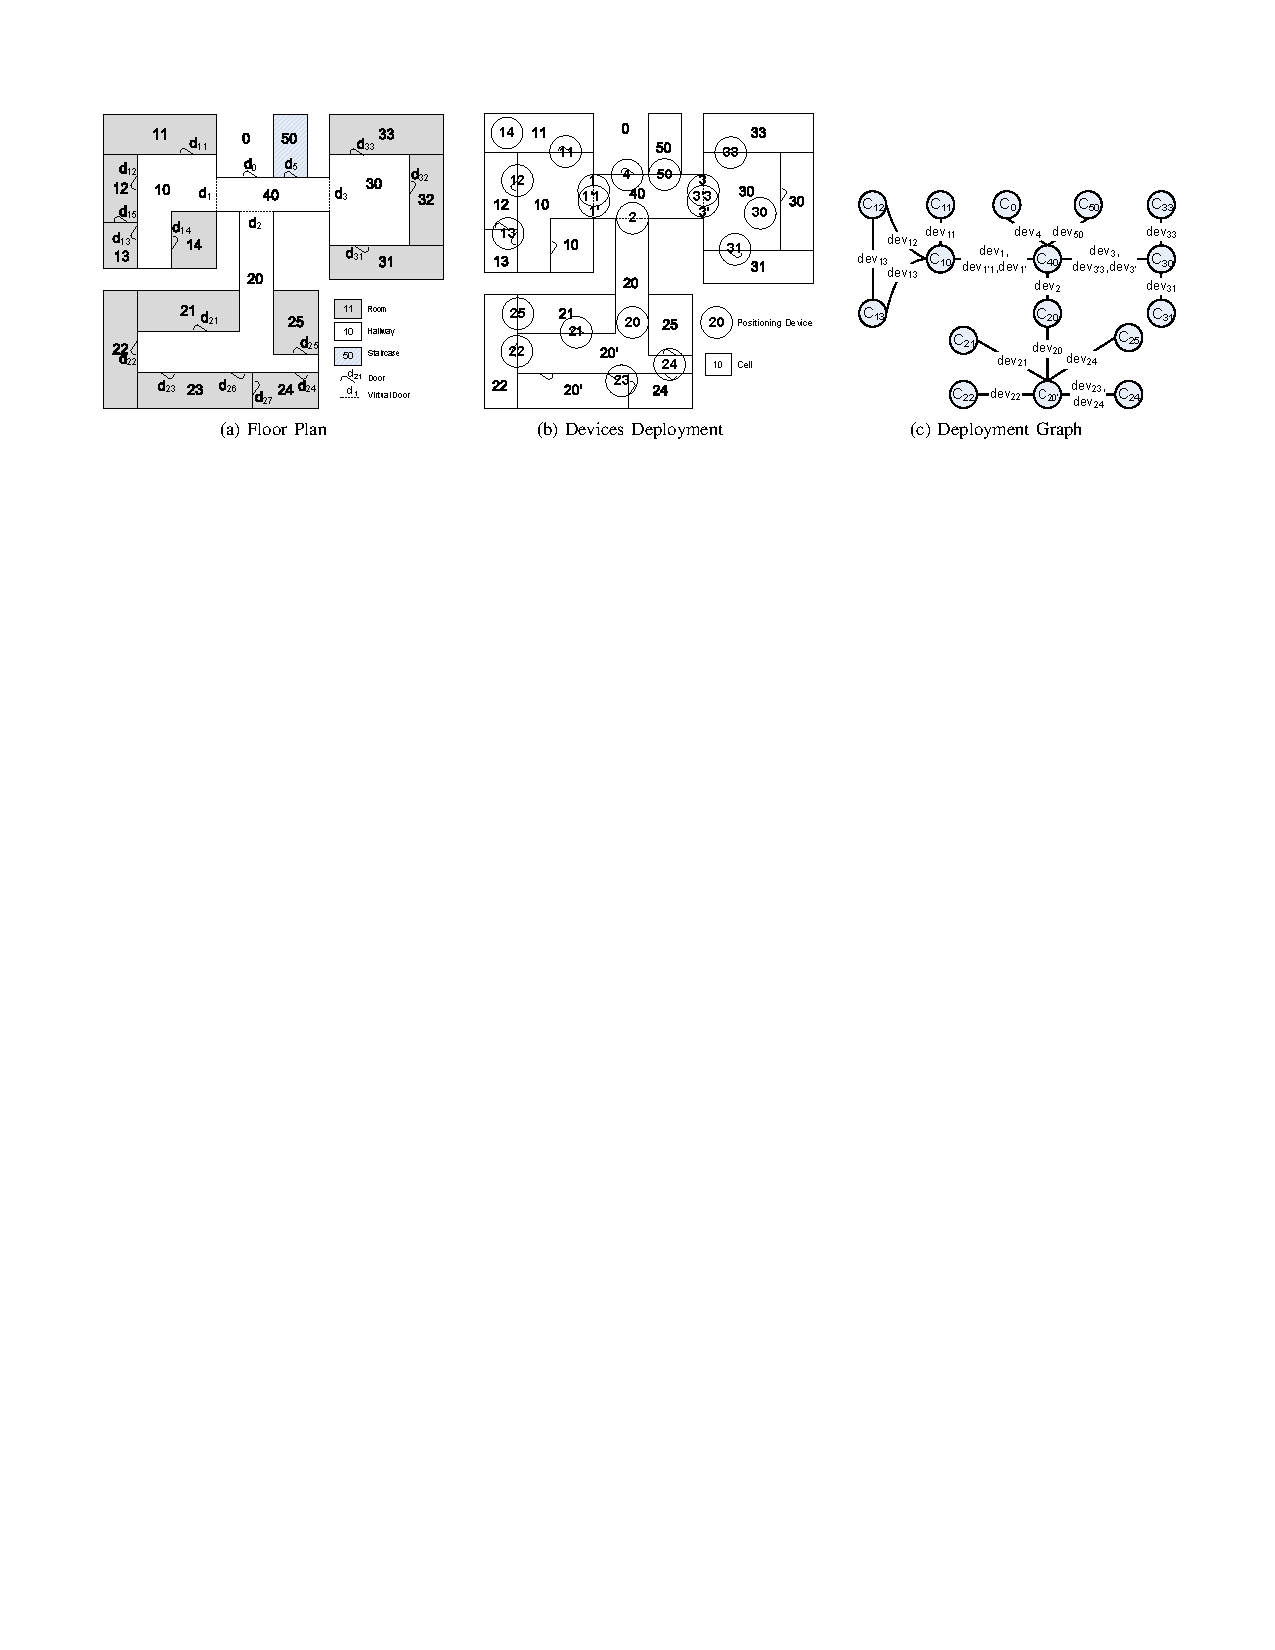
\includegraphics[width=\columnwidth]{figures/2-4/2-4-1.pdf}
\end{figure}

\begin{enumerate}
  \ssize{
  \item $\mn{C2P: C \rightarrow 2^P}$ maps a cell to a set of indoor partitions
  \item $\mn{D2C: D \rightarrow 2^C}$ maps a device to a set of corresponding cells
  \item According to Deployment Graph, for partitioning device, $\mn{D2C(device_{13})} = \{ C_{10},C_{13} \} \cup \{ C_{12},C_{13} \} = \{ C_{10},C_{12},C_{13} \}$
  \item For presence device, $\mn{D2C(device_{25})} = \{ C_{21},C_{22} \}$ as the cells intersect its detection range.
  \item $\mn{D2C: D \rightarrow 2^C}$ is useful as it captures the possible movements of objects.
  }
\end{enumerate}

\end{frame}

%------------------------------------------------

\begin{frame}
\frametitle{Preliminaries: Symbolic Indoor Tracking}

\begin{columns}[c]
  \column{.52\textwidth}
  \begin{figure}[tb]
    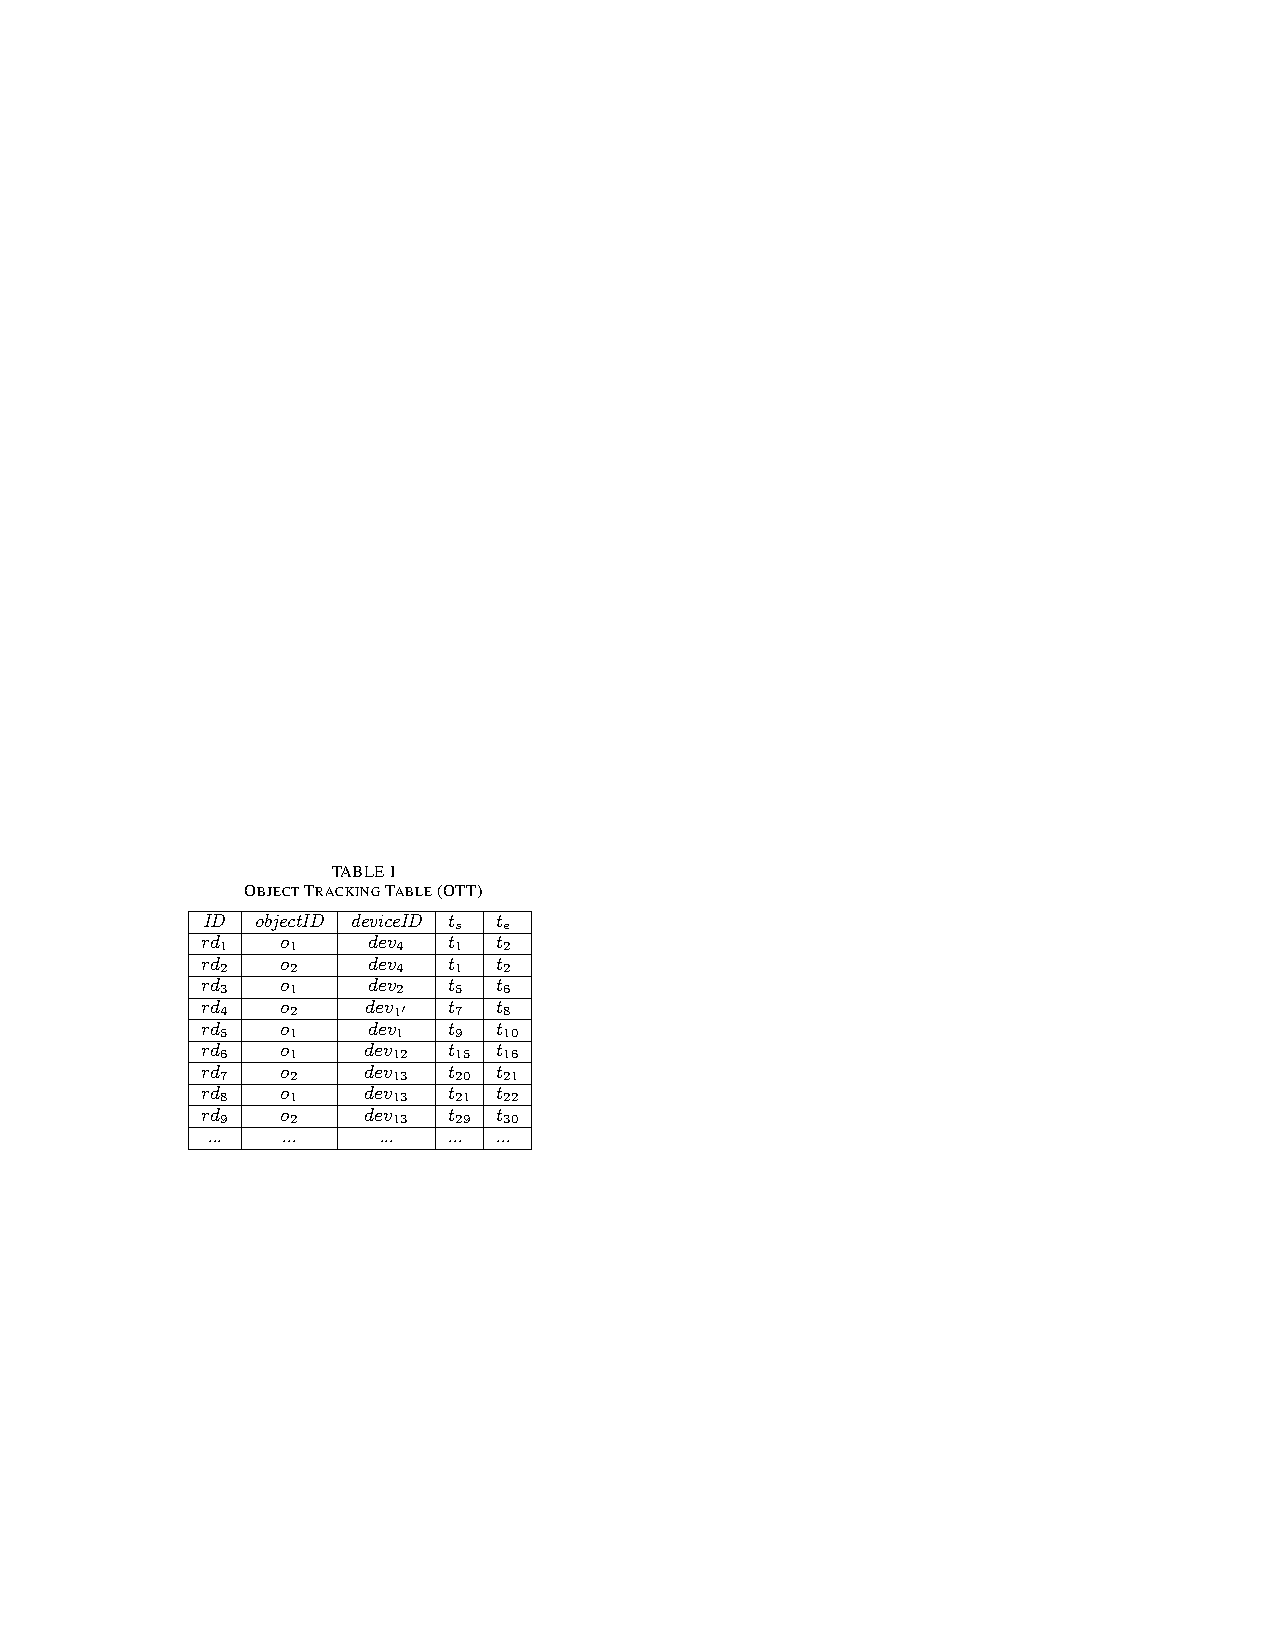
\includegraphics[width=\columnwidth]{figures/2-4/2-4-2.pdf}
  \end{figure}

  \column{.48\textwidth}
  \begin{fitemize}
    \item \conceptbf{Object Tracking Table} $\mn{OTT}$ records the converted trajectories with schema $\mn{(ID, objectID, deviceID, t_s, t_e)}$
    ~\\
    \item a record states that the object $\mn{objectID}$ is observed by the device $\mn{deviceID}$ in the closed interval from time $\mn{t_s}$ to $\mn{t_e}$.
  \end{fitemize}

\end{columns}

\end{frame}

%------------------------------------------------

\begin{frame}
\frametitle{Problem Definitions}

Given an $\mn{OTT}$, it is of interesting to identify object pairs that join w.r.t some specific spatio-temporal join predicate.
\begin{fitemize}
  \item to know all pair of individuals that were probably at the same gate when a particular event (terrorist attack) occurred in a large airport.
\end{fitemize}
~\\
Due to tracking uncertainty, only interested in those objects that satisfy the join predicate with some given probability (specified threshold).
\\~\\
The joins are effectively \emph{self-joins} because all tracking data is contained in a single $\mn{OTT}$.

\end{frame}

%------------------------------------------------

\begin{frame}
\frametitle{Problem Definition I}

\textrm{One can apply a join predicate to a time point to find pairs that join at that particular time point...}
\\~\\
\begin{definition}[\ssize{Probabilistic Threshold Indoor Spatio-temporal Join--PTISSJ}]
  \textrm{
  \ssize{
  Given an $\mn{OTT}$, a join predicate $\mn{P}$, a time point $\mn{t}$, and a threshold value $\mn{M \in (0,1]}$, a probabilistic threshold indoor spatio-temporal join  $\mn{\Join_{P,t,M}(OTT) = \{ (o_i, o_j) | o_i, o_j \in O  \wedge o_i \neq o_j \wedge pr(P(o_i, o_j, t)) >M \}}$, where $\mn{pr(P(o_i,o_j,t))}$ is the \textbf{Timeslice Join Probability} of $\mn{o_i, o_j}$ at time $\mn{t}$, i.e., the probability that predicate $\mn{P(o_i,o_j,t)}$ is true.
  }}
\end{definition}

\end{frame}

%------------------------------------------------

\begin{frame}
\frametitle{Problem Definition II}

\textrm{It's also interesting to know object pairs satisfy the predicate for some consecutive timestamp...}
\\~\\
\begin{definition}[\ssize{Probabilistic Threshold $k$ Indoor Spatio-temporal Join--PT$k$ISSJ}]
  \textrm{
  \ssize{
  Given an $\mn{OTT}$, a join predicate $\mn{P}$, a time interval $\mn{I = [t_m, t_n] (m < n)}$, an integer $\mn{k(0 < k \leq n - m)}$, and a threshold value $\mn{M \in (0,1]}$, a probabilistic $\mn{k}$ threshold indoor spatio-temporal join
  \begin{equation*}
    \begin{split}
    &\mn{\Join_{P,I,k,M}(OTT) = \{ (o_i, o_j) | o_i, o_j \in O \wedge o_i \neq o_j \wedge } \\
    &\mn{\exists s \in m...n -k + 1 (\forall\delta \in 0...k-1 (pr(P(o_i, o_j, t_{s+\delta})) > M)) \} }
    \end{split}
  \end{equation*}
  }}
\end{definition}

\end{frame}

%------------------------------------------------

\begin{frame}
\frametitle{Uncertainty Model for Indoor Tracking}

\textrm{For outdoor moving objects~\cite{cheng2004querying}, \conceptbf{Uncertainty Region}, denoted by $\mn{UR(o_i,t)}$, is a region such that $\mn{o_i}$ must be in this region at time $\mn{t}$.}\\~

In general terms, an object $\mn{o_i}$'s location can be modeled as a random variable $\mn{l}$ associated with a probability density function $\mn{f_{o_i}(l,t)}$ that has non-zero values only in $\mn{o_i}$'s suncertainty region $\mn{UR(o_i, t)}$.~\cite{DBLP:conf/edbt/YangLJ10}

\begin{equation}
  \mn{\int_{l \in UR(o_i,t)} f_{o_i}(l,t) dl = 1}
\end{equation}

\end{frame}

%------------------------------------------------

\begin{frame}
\frametitle{Object State in OTT}

\begin{columns}[c]

\column{.45\textwidth}
\begin{figure}[tb]
  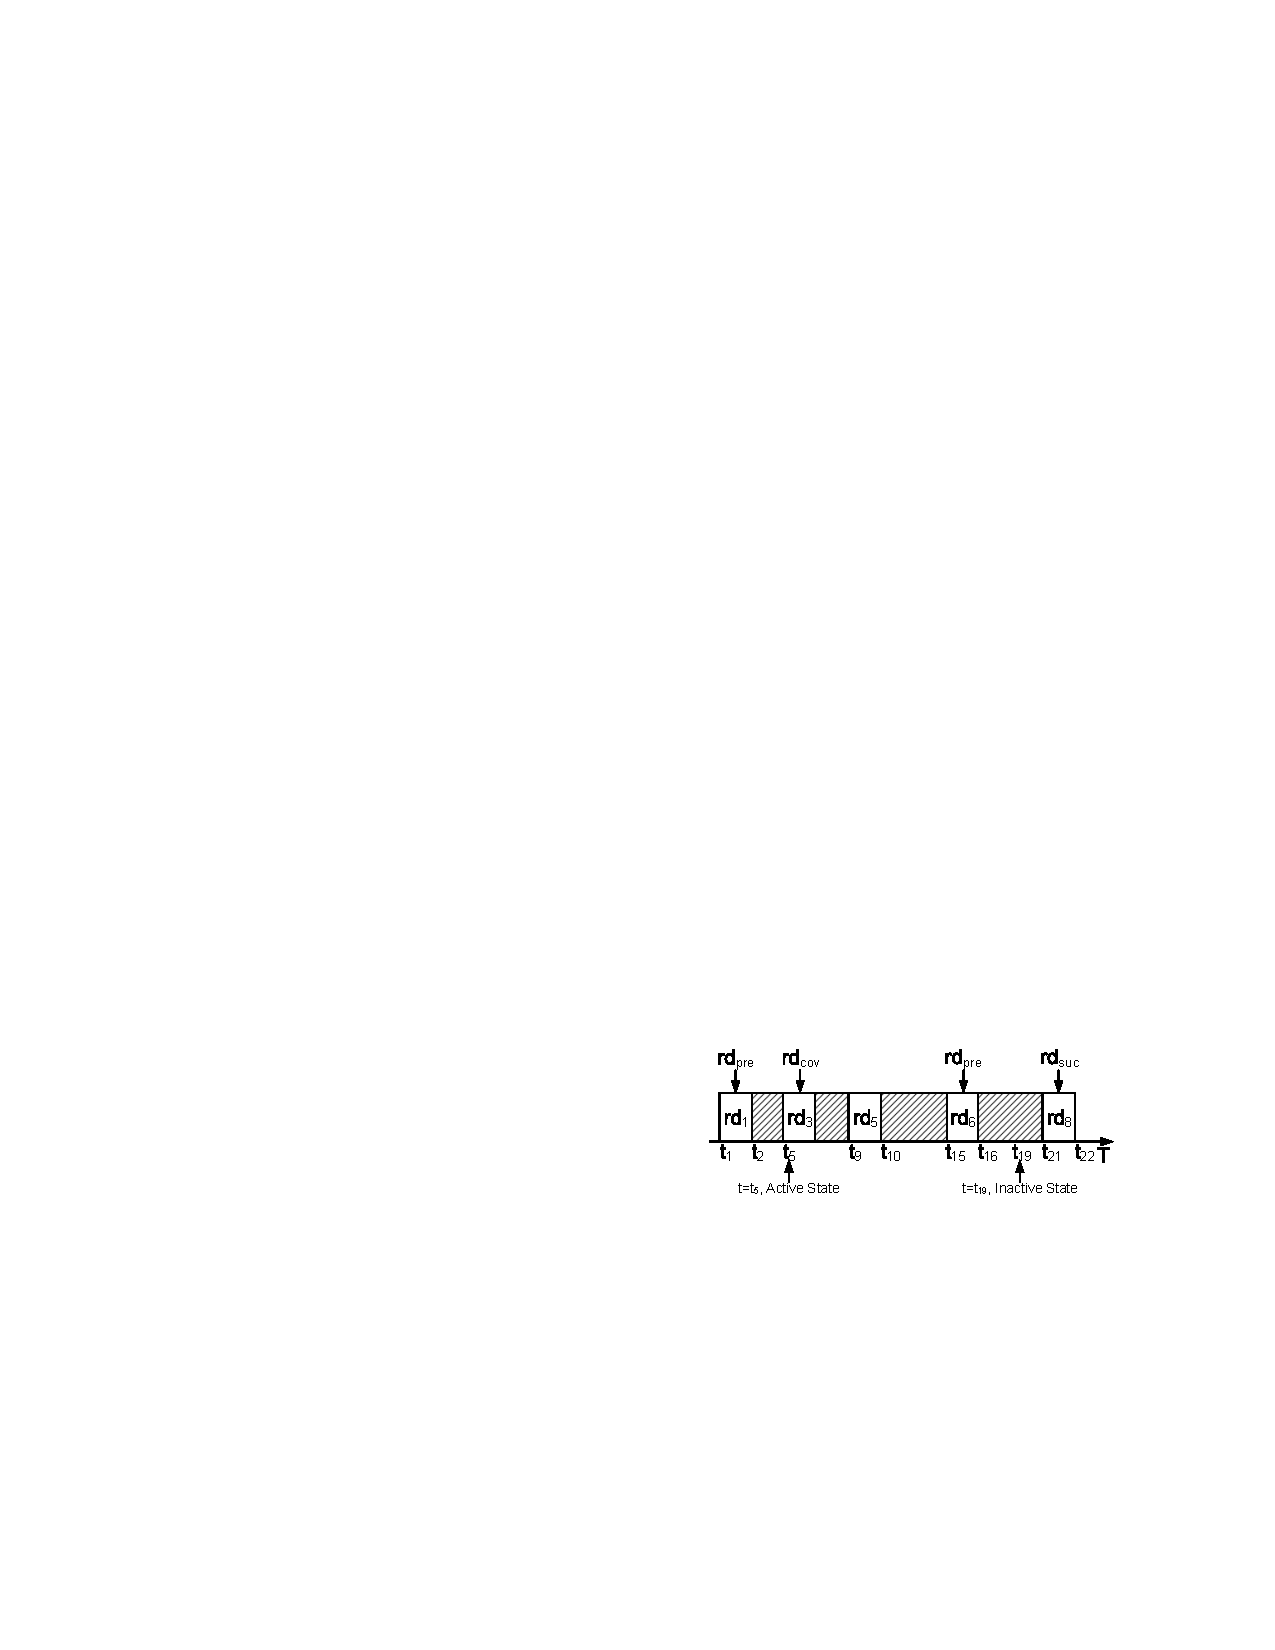
\includegraphics[width=\columnwidth]{figures/2-4/2-4-3.pdf}
\end{figure}

\column{.55\textwidth}
\begin{definition}[Active State]
  \textrm{
  \ssize{
  Given an object $\mn{o_i}$ and a time point $\mn{t}$, if a tracking record $\mn{rd_{cov}}$ is found in $\mn{OTT}$ such that $\mn{rd_{cov}.objectID = o_i}$ and $\mn{t \in [rd_{cov}.t_s, rd_{cov}.t_e]}$, $\mn{o_i}$ is in the \conceptbf{active state} at time $\mn{t}$.
  }}
\end{definition}

\end{columns}

\begin{definition}[Inactive State]
  \textrm{
  \ssize{
  Given an object $\mn{o_i}$ and a time point $\mn{t}$, if no record $\mn{rd_{cov}}$ is found in $\mn{OTT}$, $\mn{o_i}$ is in the \conceptbf{inactive state} at time $\mn{t}$. Instead, two tracking records of $\mn{o_i}$ called $\mn{rd_{pre}}$ and $\mn{rd_{suc}}$, can be found in $\mn{OTT}$, such that they are consecutive in the sense that $\mn{rd_{pre}.t_e < t < rd_{suc}.t_s}$ and there is no record for $\mn{o_i}$ between times $\mn{rd_{pre}.t_e}$ and $\mn{rd_{suc}.t_s}$.
  }}
\end{definition}

\end{frame}

%------------------------------------------------

\begin{frame}
\frametitle{Uncertainty Region in the Active State}

\begin{columns}[c]
  \column{.52\textwidth}
  \vspace{-10pt}
  \begin{figure}[tb]
    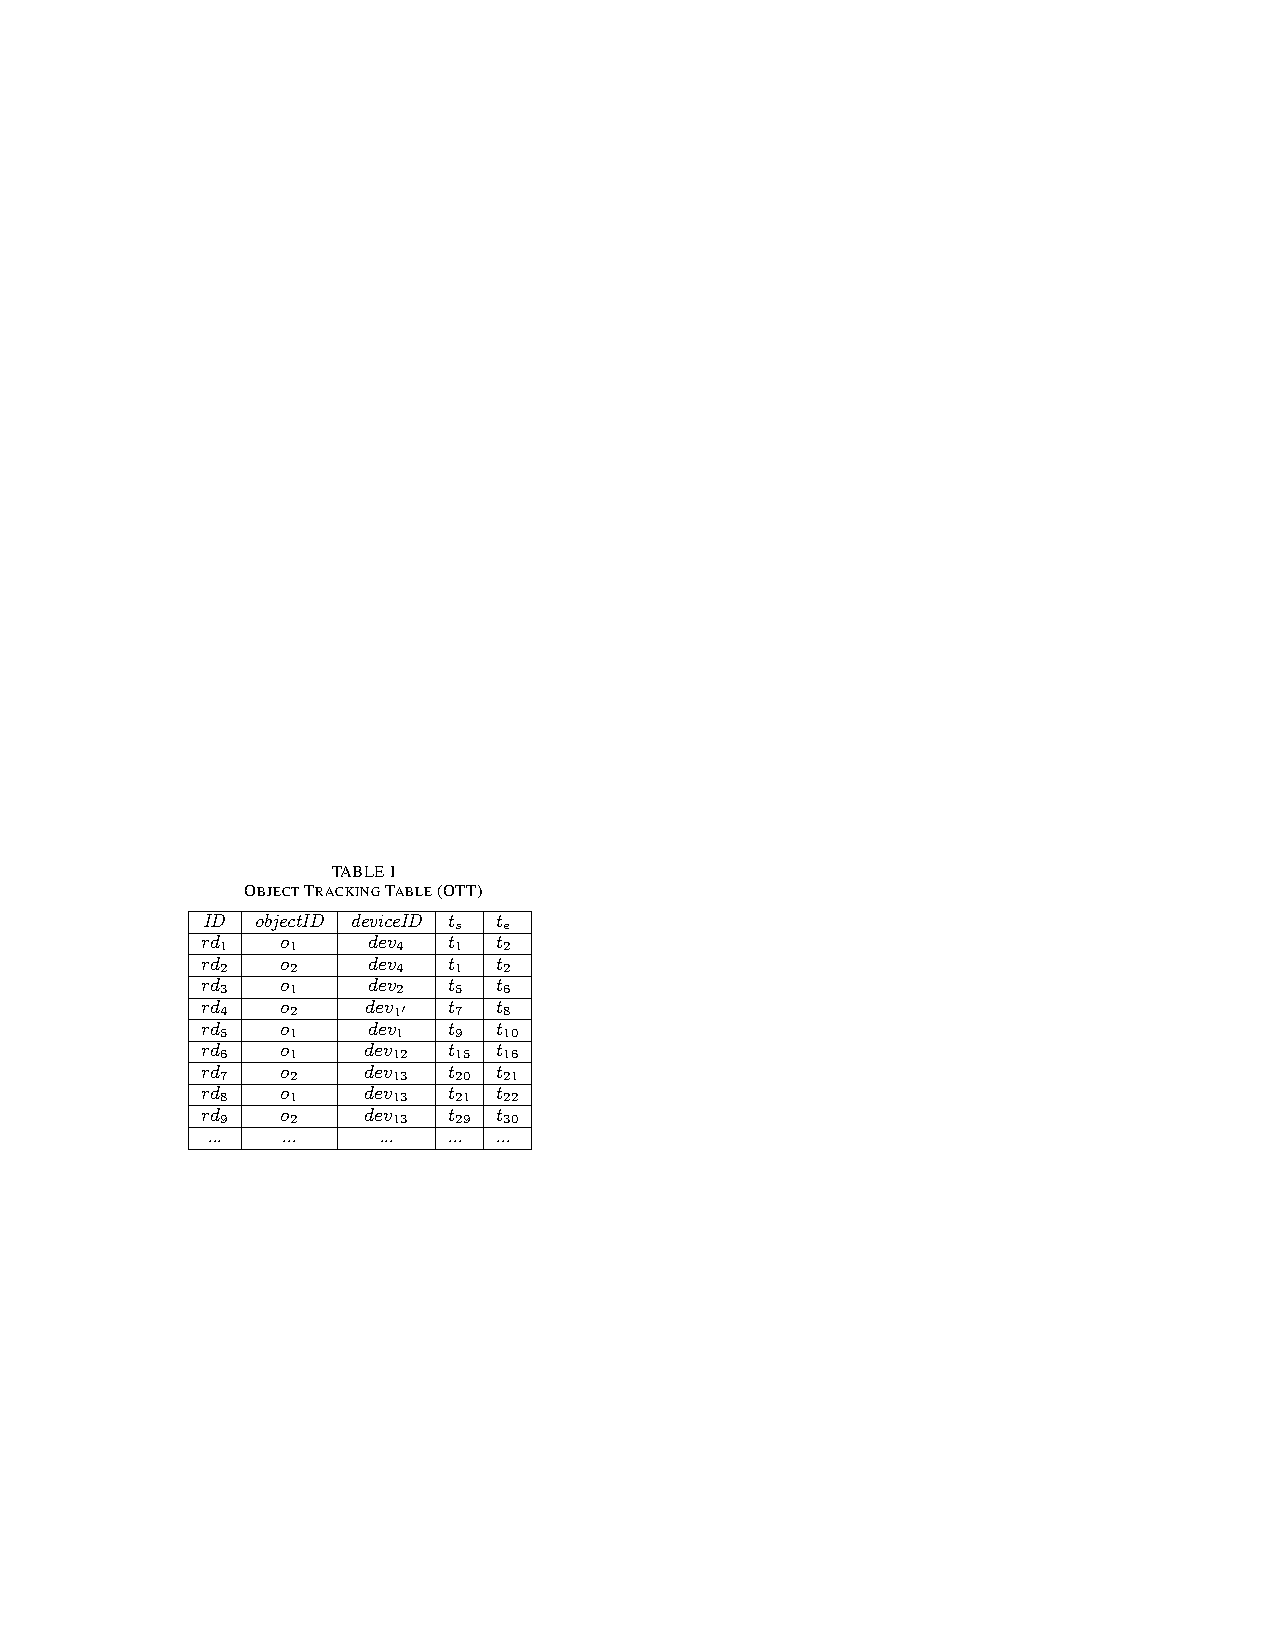
\includegraphics[width=\columnwidth]{figures/2-4/2-4-2.pdf}
  \end{figure}
  \vspace{-15pt}
  \begin{example}
    \textrm{
    \ssize{
    $\mn{t = t_5}$, $\mn{rd_{cov} = rd_3}$ and $\mn{rd_{pre} = rd_1}$, which tells $\mn{o_i}$ left $\mn{dev_4}$'s detection range at time $\mn{t_2}$, and is currently detected by $\mn{dev_2}$.
    }}
  \end{example}

  \column{.48\textwidth}
  \vspace{-10pt}
  \begin{figure}[tb]
    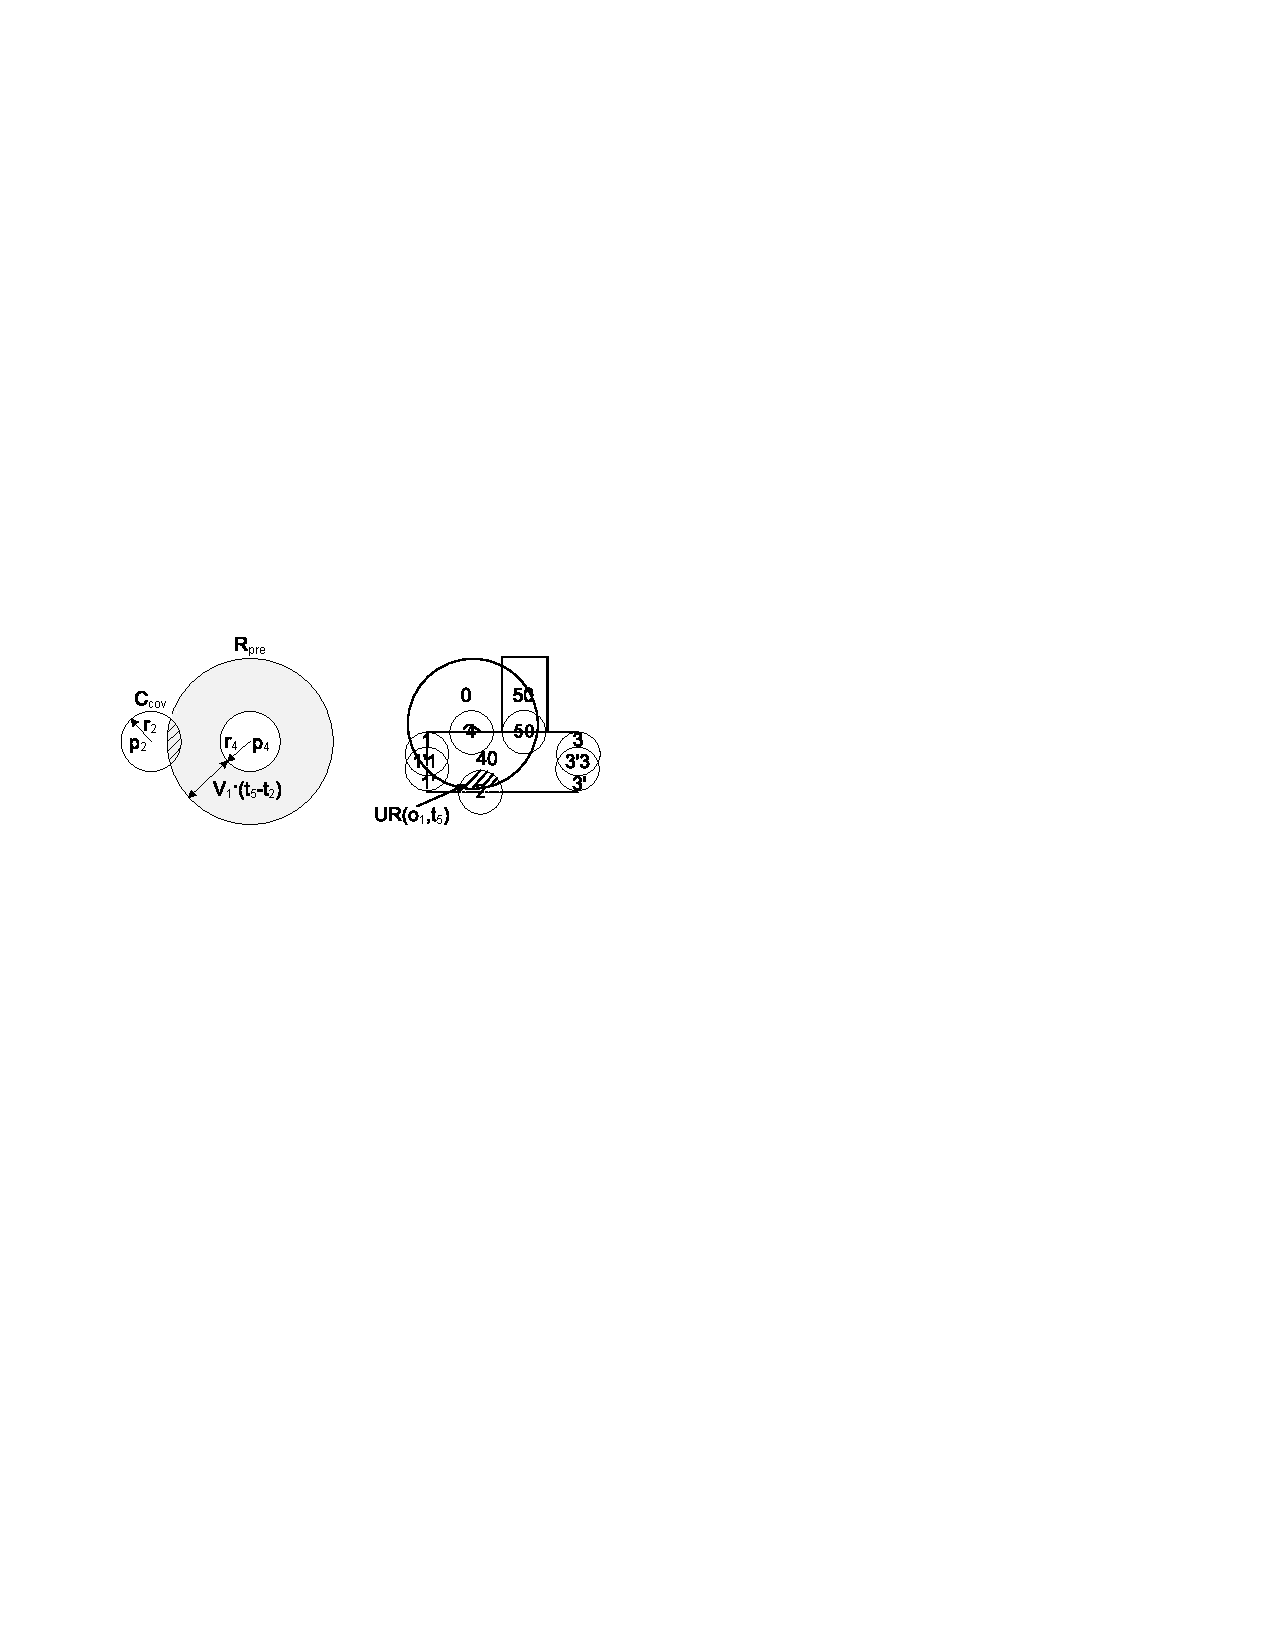
\includegraphics[width=\columnwidth]{figures/2-4/2-4-4.pdf}
  \end{figure}
  \ssize{
  \textbf{Step 1:}
  UR is the detection range of device $\mn{rd_{cov}.deviceID}$, denote as:
  \begin{equation*}
  \begin{split}
    \mn{ C_{cov} = } &\mn { Cir(Loc(rd_{cov}.deviceID), }\\
    &\mn{ Rad(rd_{cov}.deviceID)) }
  \end{split}
  \end{equation*}
  ~\\
  \textbf{Step 2:}
  UR should consider the $\mn{rd_{pre}}$'s \emph{maximum speed bounding ring}(MSBR):
  \tiny{
  \begin{equation*}
  \begin{split}
    &\mn{ UR(o_i, t) = C_{cov} \cap Ring(Loc(rd_{pre}.deviceID), } \\
    &\mn{ Rad(rd_{pre}.deviceID), V_i \cdot (t - rd_{pre}.t_e) ) }
  \end{split}
  \end{equation*}
  }
  }
\end{columns}

\end{frame}

%------------------------------------------------

\begin{frame}
\frametitle{Uncertainty Region in the Inactive State}

\begin{columns}[c]

  \column{.52\textwidth}
  \vspace{-10pt}
  \begin{figure}[tb]
    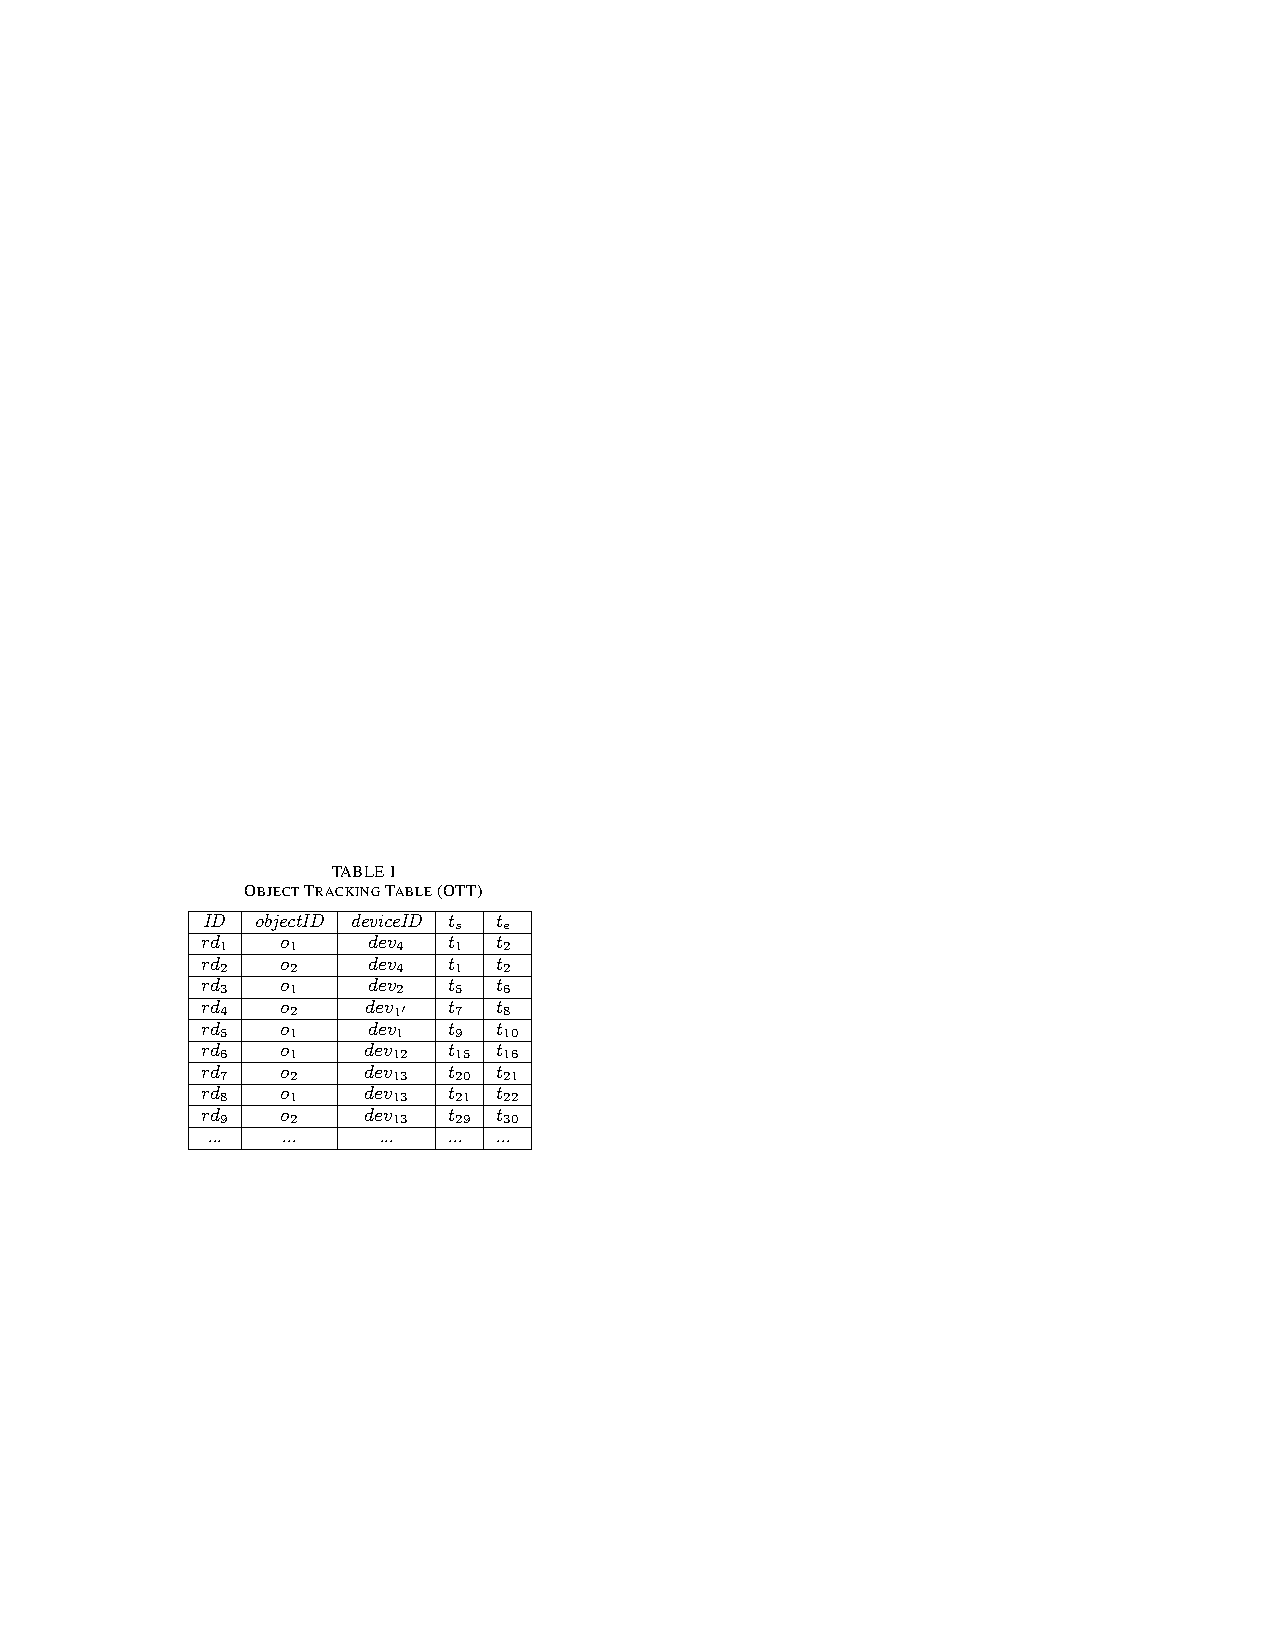
\includegraphics[width=\columnwidth]{figures/2-4/2-4-2.pdf}
  \end{figure}
  \vspace{-15pt}
  \begin{example}
    \textrm{
    \ssize{
    $\mn{t = t_{19}}$, $\mn{rd_{pre} = rd_6}$ and $\mn{rd_{suc} = rd_8}$, since $\mn{rd_6.t_e = t_{16} < t_{19} < rd_8.t_s = t_{21}}$. we have $\mn{dev_p = dev_{12}}$ and $\mn{dev_s = dev_{13}}$
    }}
  \end{example}

  \column{.48\textwidth}
  \vspace{-10pt}
  \begin{figure}[tb]
    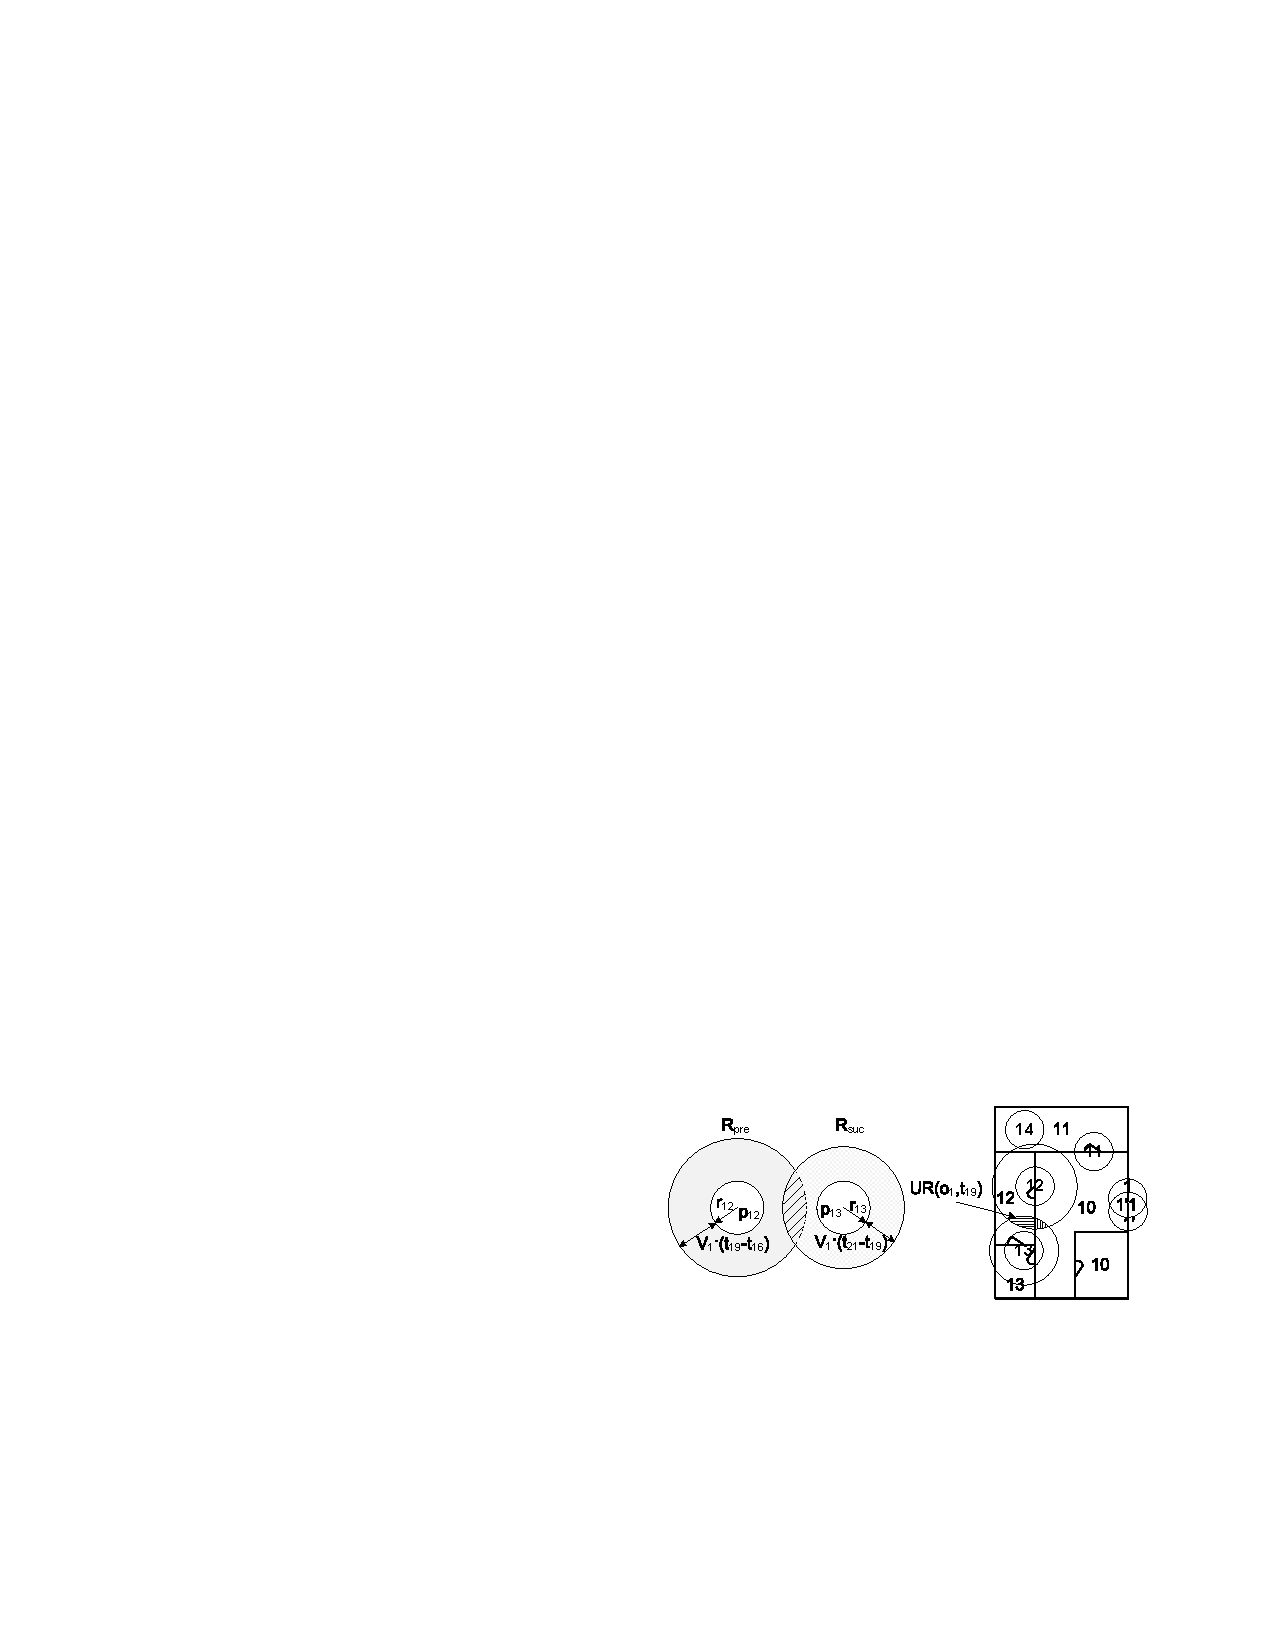
\includegraphics[width=\columnwidth]{figures/2-4/2-4-5.pdf}
  \end{figure}
  \ssize{
  \textbf{Step 1:}
  Determine the possible cells in which the object can be in the inactive period:
  \begin{equation*}
    \mn{ Cells_{mid} = D2C(dev_p) \cup D2C(dev_s)}
  \end{equation*}
  ~\\
  \textbf{Step 2:}
  UR is constrained by two \emph{maximum speed bounding ring}(MSBR)s of $\mn{rd_{pre}}$ and $\mn{rd_{suc}}$:
  \tiny{
  \begin{equation*}
  \begin{split}
    \mn{ UR(o_i, t) = \bigcup_{c \in Cells_{mid}} c \cap R_{pre} \cap R_{suc} }
  \end{split}
  \end{equation*}
  }
  }
\end{columns}

\end{frame}

%------------------------------------------------

\begin{frame}
\frametitle{Join Probability Evaluation}

\begin{definition}[the \emph{same X} predicate]
  \textrm{
  \ssize{
    termed as $\mn{P_X}$, where $\mn{X}$ represents an indoor region type. $\mn{IR_X}$ represents all $\mn{X}$ type regions ($\mn{X}$-regions).
  }
  }
\end{definition}
~\\
\begin{example}[the \emph{same room} predicate]
  \textrm{
  \ssize{
    Given two objects $\mn{o_i, o_j}$ at a time point $\mn{t}$, the \emph{same room} predicate $\mn{P_X(o_i, o_j, t)}$ evaluates to true if both $\mn{o_i, o_j}$ were located in a same room $\mn{rm \in IR_X}$. Other predicates can be \emph{same floor, same reserach group (maps to several rooms)}.
  }
  }
\end{example}
~\\
The \emph{same X} predicates are more practical than Euclidean distance based join predicates in indoor space.

\end{frame}

%------------------------------------------------

\begin{frame}
\frametitle{Join Probability Evaluation}
\vspace{-10pt}
\begin{definition}[``be located at'' predicate probability]
  \textrm{
  \ssize{
    Given an object $\mn{o_i}$, an $\mn{X}$-region $\mn{x_l \in IR_X}$, and a time $\mn{t}$, predicate $\Theta(o_i, x_l, t)$ indicate that $\mn{o_i}$ was located in $\mn{x_l}$ at $\mn{t}$. The probability that $\mn{\Theta}$ is satisfied is defined as:
    \begin{equation*}
      \mn{pr(\Theta(o_i, x_l, t)) = \frac{Area(UR(o_i, t) \cap x_l)}{Area(UR(o_i, t))}}
    \end{equation*}
  }
  }
\end{definition}

\begin{definition}[the \emph{same X} predicate probability]
  \textrm{
  \ssize{
    The probability that $\mn{o_i}$ and $\mn{o_j}$ were located in the same $\mn{x_l}$ at $\mn{t}$, indicated by $\mn{pr(P_{x_l}(o_i, o_j, t))}$ is defined as:
    \begin{equation*}
      \mn{pr(P_{x_l}(o_i, o_j, t)) = pr(\Theta(o_i, x_l, t)) \cdot pr(\Theta(o_j, x_l, t)) }
    \end{equation*}
    Therefore, the porbability that $\mn{o_i}$ and $\mn{o_j}$ satisfy a \emph{same X} predicate at time $\mn{t}$ can be defined as:
    \begin{equation*}
      \mn{pr(P_X(o_i, o_j, t)) = \max_{x_l \in IR_X} pr(P_{x_l}(o_i, o_j, t)) }
    \end{equation*}
  }
  }
\end{definition}

\end{frame}

%------------------------------------------------

\begin{frame}
\frametitle{Indexing the Indoor Tracking Data}

\textrm{to determine the \emph{Uncertainty Region} during join processing, it needs to retrieve the records $\mn{rd_{cov}}$ and $\mn{rd_{pre}}$ for active objects or $\mn{rd_{pre}}$ and $\mn{rd_{suc}}$ for inactive state.}
\\~\\
to index $\mn{OTT}$ with an augmented 1D R-tree, where each leaf entry has the form $\mn{(t^{\vdash},t^{\dashv},Ptr_{p},Ptr_{c})}$. $\mn{t^{\vdash} = rd_p.t_e}$, $\mn{t^{\dashv} = rd_c.t_e}$, $\mn{Ptr_p}$ and $\mn{Ptr_c}$ points to $\mn{rd_p}$ and $\mn{rd_c}$ respectively.

\begin{fitemize}
  \item if $\mn{t \geq rd_c.t_s}$, $\mn{o_i}$ is active, $\mn{rd_p \rightarrow rd_{pre}}$ and $\mn{rd_c \rightarrow rd_{cov}}$;
  \item if $\mn{t < rd_c.t_s}$, $\mn{o_i}$ is inactive, $\mn{rd_p \rightarrow rd_{pre}}$ and $\mn{rd_c \rightarrow rd_{suc}}$;
\end{fitemize}

\end{frame}

%------------------------------------------------

\begin{frame}
\frametitle{Accessing $\mn{X}$-Regions}

\textrm{object locations are bounded by either device detection ranges or cells.}

\begin{columns}[c]

  \column{.54\textwidth}
  \begin{figure}[tb]
    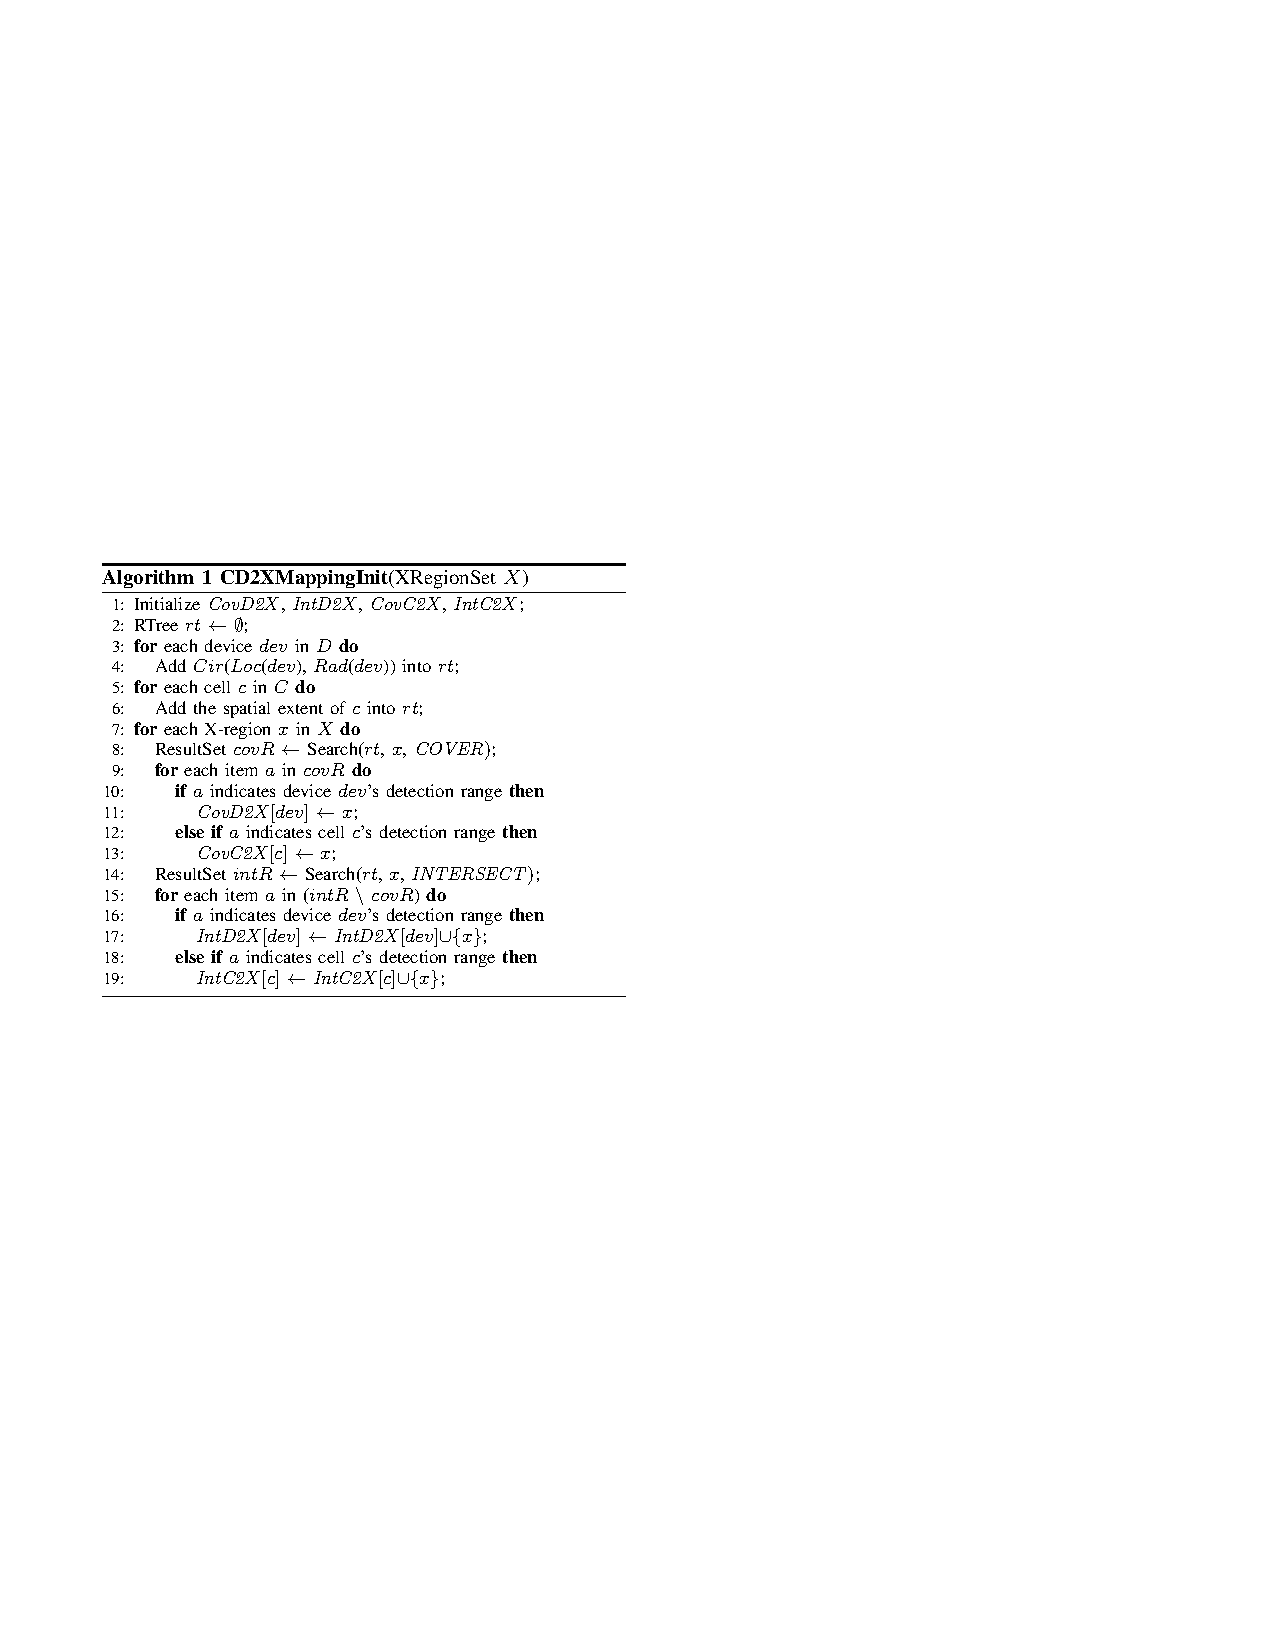
\includegraphics[width=\columnwidth]{figures/2-4/2-4-6.pdf}
  \end{figure}

  \column{0.48\textwidth}
  \begin{sitemize}
    \item $\mn{CovD2X: D \rightarrow IR_X}$ maps a device to an $\mn{X}$-Region that fully covers the device's detection range;
    \item $\mn{IntD2X: D \rightarrow IR_X}$ maps a device to an $\mn{X}$-Region that only intersects the device's detection range;
    \item $\mn{CovC2X: C \rightarrow IR_X}$ maps a cell to an $\mn{X}$-Region that fully covers this cell;
    \item $\mn{IntC2X: C \rightarrow IR_X}$ maps a cell to an $\mn{X}$-Region that only intersects with;
  \end{sitemize}

\end{columns}

\end{frame}

%------------------------------------------------

\begin{frame}
\frametitle{Processing PTISSJ Queries: Partitioning Phase}

\begin{columns}[c]

  \column{.47\textwidth}
  \vspace{-10pt}
  \begin{figure}[tb]
    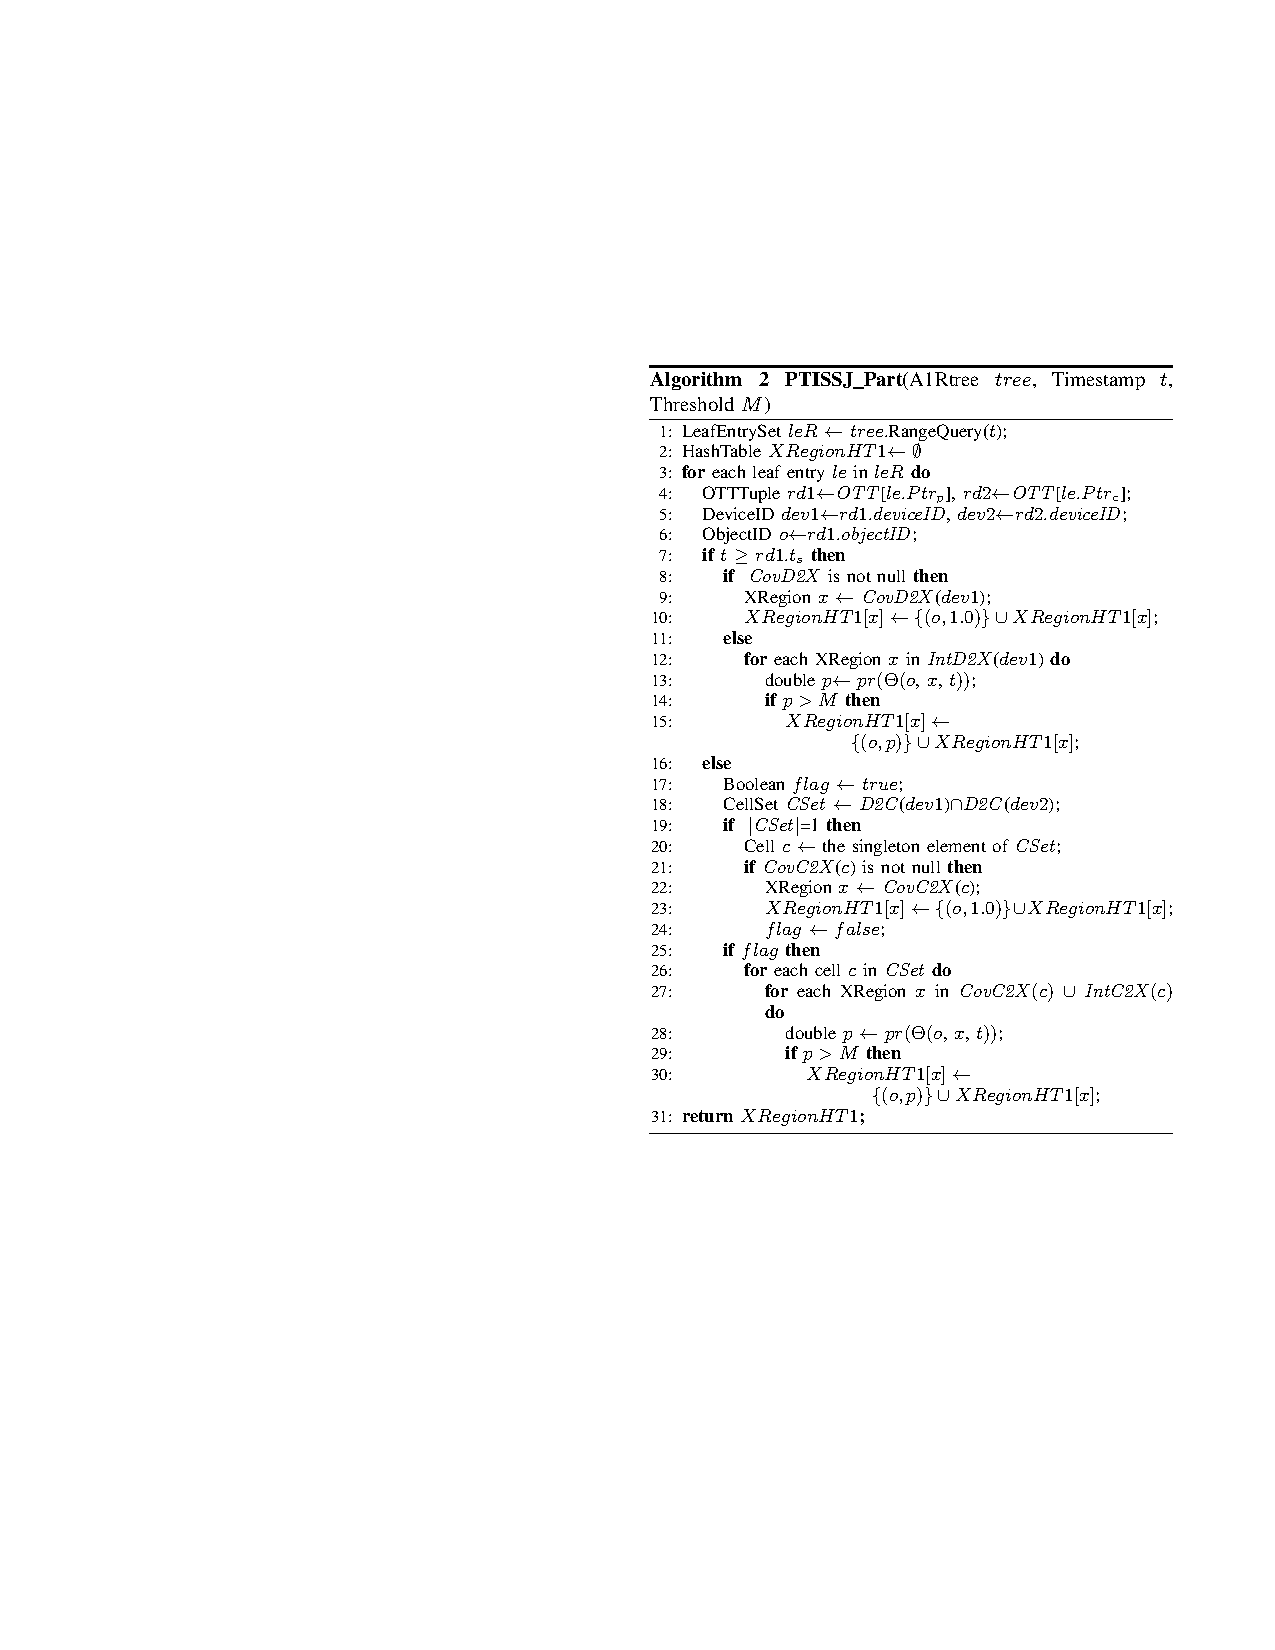
\includegraphics[width=\columnwidth]{figures/2-4/2-4-7.pdf}
  \end{figure}

  \column{0.53\textwidth}
  \begin{fitemize}
    \item all indoor objects are partitioned into buckets that each refers to a distinct $\mn{X}$-region
    \item first, A1R-tree is searched to get all leaf entries whose interval $\mn{(t^{\vdash},t^{\dashv}]}$ contains the join time $\mn{t}$
    \item second, the spatial examination obtains all relevant $\mn{X}$-region in which $\mn{o_i}$ may be at time $\mn{t}$
    \item the relevant probabilities are evaluated for each object, and the necessary records are generated and added to relevant buckets, for each $\mn{p_l = pr(\Theta(o_i, x_l, t))}$, if it is larger than threshold $\mn{M}$, insert the record into buckets.
  \end{fitemize}

\end{columns}

\end{frame}

%------------------------------------------------

\begin{frame}
\frametitle{Processing PTISSJ Queries: Partitioning Phase}

\begin{columns}[c]

  \column{.5\textwidth}
  \textbf{Active State}~\\
  \ssize{
  \textrm{object $\mn{o_i}$ must be in device $\mn{dev}$'s detection range at time $\mn{t}$}.~\\
  \begin{enumerate}
    \item if the detection range is fully covered by an $\mn{X}$-region $\mn{x_l}$, as indicated by $\mn{CovD2X(dev_c) = x_l}$, a record $\mn{(o_i, 1.0)}$ is added to $\mn{x_l}$'s bucket;
    \item otherwise, $\mn{dev_c}$'s detection range intersects with each $\mn{X}$-region in $\mn{CovD2X(dev_c)}$, evaluated the probability, if it is larger than $\mn{M}$, add to the bucket.
  \end{enumerate}
  }

  \column{0.5\textwidth}
  \textbf{Inactive State}~\\
  \ssize{
  \textrm{object $\mn{o_i}$ must be in a cell in $\mn{Cells_{mid} = D2C(dev_p) \cap D2C(dev_c)}$}.~\\
  \begin{enumerate}
    \item if $\mn{Cells_{mid}}$ is the singleton set and the cell is covered by one $\mn{X}$-region $\mn{x_l}$, indicated by $\mn{CovC2X(c)= x_l}$, a record $\mn{(o_i, 1.0)}$ is added to $\mn{x_l}$'s bucket;
    \item otherwise, the single cell $\mn{c}$ in $\mn{Cells_{mid}}$ intersects with several $\mn{X}$-regions (indicated by $\mn{CovC2X(c)}$), or $\mn{Cells_{mid}}$ contains several cells.
  \end{enumerate}
  }

\end{columns}

\end{frame}

% \begin{frame}[allowframebreaks]
\frametitle{References}

\begin{thebibliography}{99} % Beamer does not support BibTeX so references must be inserted manually as below
\fsize{

\bibitem{DBLP:conf/mdm/JensenLY09}
C.S.~Jensen, H.~Lu, B.~Yang.
\newblock Graph model based indoor tracking.
\newblock In {\em {MDM}}, pp. 122--131, 2009.

\bibitem{DBLP:conf/cikm/YangLJ09}
B.~Yang, H.~Lu, C.S.~Jensen.
\newblock Scalable continuous range monitoring of moving objects in symbolic
  indoor space.
\newblock In {\em CIKM}, pp. 671--680, 2009.

\bibitem{DBLP:conf/edbt/YangLJ10}
B.~Yang, H.~Lu, C.S.~Jensen.
\newblock Probabilistic threshold k nearest neighbor queries over moving
  objects in symbolic indoor space.
\newblock In {\em EDBT}, pp. 335--346, 2010.

\bibitem{DBLP:conf/icde/LuYCJ11}
H.~Lu, B.~Yang, C.S.~Jensen.
\newblock Spatio-temporal Joins on Symbolic Indoor Tracking Data.
\newblock In {\em {ICDE}}, pp. 816--827, 2011.

\bibitem{jensen2010indoor}
C.S.~Jensen, H.~Lu, B.~Yang.
\newblock Indoor-A New Data Management Frontier.
\newblock In {\em IEEE Data Eng. Bull.}, pp. 12--17, 2010.

\bibitem{cheng2004querying}
R.~Cheng, D.V.~Kalashnikov, S.~Prabhakar.
\newblock Querying imprecise data in moving object environments.
\newblock In {\em TKDE}, pp. 1112--1127, 2004.

\bibitem{pfoser1999capturing}
D.~Pfoser, C.S.~Jensen.
\newblock Capturing the uncertainty of moving-object representations
\newblock In {\em Advances in Spatial Databases}, pp. 111--131, 1999.

}
\end{thebibliography}

\end{frame}


\subsection{2.5 A Foundation for Efficient Indoor Distance-aware Query Processing} % A subsection can be created just before a set of slides with a common theme to further break down your presentation into chunks

% \begin{frame}
\frametitle{About This Work...}

\emph{A Foundation for Efficient Indoor Distance-Aware Query Processing}.~\cite{DBLP:conf/icde/LuYCJ11} \\
H.~Lu, X.~Cao, and C.~S. Jensen.\\~\\

\begin{itemize}
  \item Published at \emph{ICDE' 2012}.
  \item First time to propose a distance-aware indoor space model that integrates indoor distance seamlessly.
  \item Accompanying, efficient algorithms for computing indoor distances.
  \item Indexing framework that accommodates indoor distances.
\end{itemize}

\end{frame}

%------------------------------------------------

\begin{frame}
\frametitle{Motivation}

\begin{itemize}
  \item A variety of LBS services are useful in indoor space.
    \begin{fitemize}
      \item a museum guidance service in a complex exhibition
      \item boarding reminder service in an airport, to remind the passengers especially those far away from their gates or departures
    \end{fitemize}

  \item Such indoor LBSs will benefit from the availability of accurate indoor distances.
    \begin{fitemize}
      \item indoor space entities enable as well as constrain indoor movement, thus makes traditional space model for Euclidean/spatial network spaces unsuitable.
      \item existing indoor space models~\cite{becker2005location, li2008lattice, becker2009multilayered} pay little attention to indoor distances.
    \end{fitemize}

\end{itemize}

\end{frame}

%------------------------------------------------

\begin{frame}
\frametitle{Indoor Topology Mapping Structures}

Mapping $D2P$ maps a door $d_k$ to one or two partition pairs~\footnote{\ssize{the basic assumption that a door corresponds to two doors can be extended by converting a door to multiple doors.}} $(v_i, v_j)$ such that one can move from partition~\footnote{\ssize{a partition indicates a room, a hallway or a staircase.}} $v_i$ to partition $v_j$ through door $d_k$:
\pause
\begin{equation}
 D2P: \mathcal{S}_{door} \rightarrow 2^{\mathcal{S}_{partition}} \times 2^{\mathcal{S}_{partition}}
\end{equation}
\pause
For \emph{enterable partition} of door $d_k$:
\pause
\begin{equation}
 D2P_{\sqsupset}: \mathcal{S}_{door} \rightarrow 2^{\mathcal{S}_{partition}}
\end{equation}
\pause
For \emph{leaveable partition} of door $d_k$:
\pause
\begin{equation}
 D2P_{\sqsubset}: \mathcal{S}_{door} \rightarrow 2^{\mathcal{S}_{partition}}
\end{equation}
\end{frame}

%------------------------------------------------

\begin{frame}
\frametitle{Indoor Topology Mapping Structures}


The mapping $P2D_{\sqsupset}$ maps a partition $v$ to all the doors through which one can enter $v$:
\pause
\begin{equation}
 P2D_{\sqsupset}: \mathcal{S}_{partition} \rightarrow 2^{\mathcal{S}_{door}}
\end{equation}
\pause
The mapping $P2D_{\sqsubset}$ maps a partition $v$ to all the doors through which one can leave $v$:
\pause
\begin{equation}
 P2D_{\sqsubset}: \mathcal{S}_{partition} \rightarrow 2^{\mathcal{S}_{door}}
\end{equation}
\pause
The mapping $P2D$ is used when there's no need to differentiate the directionality:
\pause
\begin{equation}
 P2D(v_i): P2D_{\sqsupset}(v_i) \cup P2D_{\sqsubset}(v_i)
\end{equation}
\end{frame}

%------------------------------------------------

\begin{frame}
\frametitle{Accessibility Base Graph}

\begin{columns}[c]

  \column{0.52\textwidth}
  \vspace{-15pt}
  \begin{figure}[tb]
    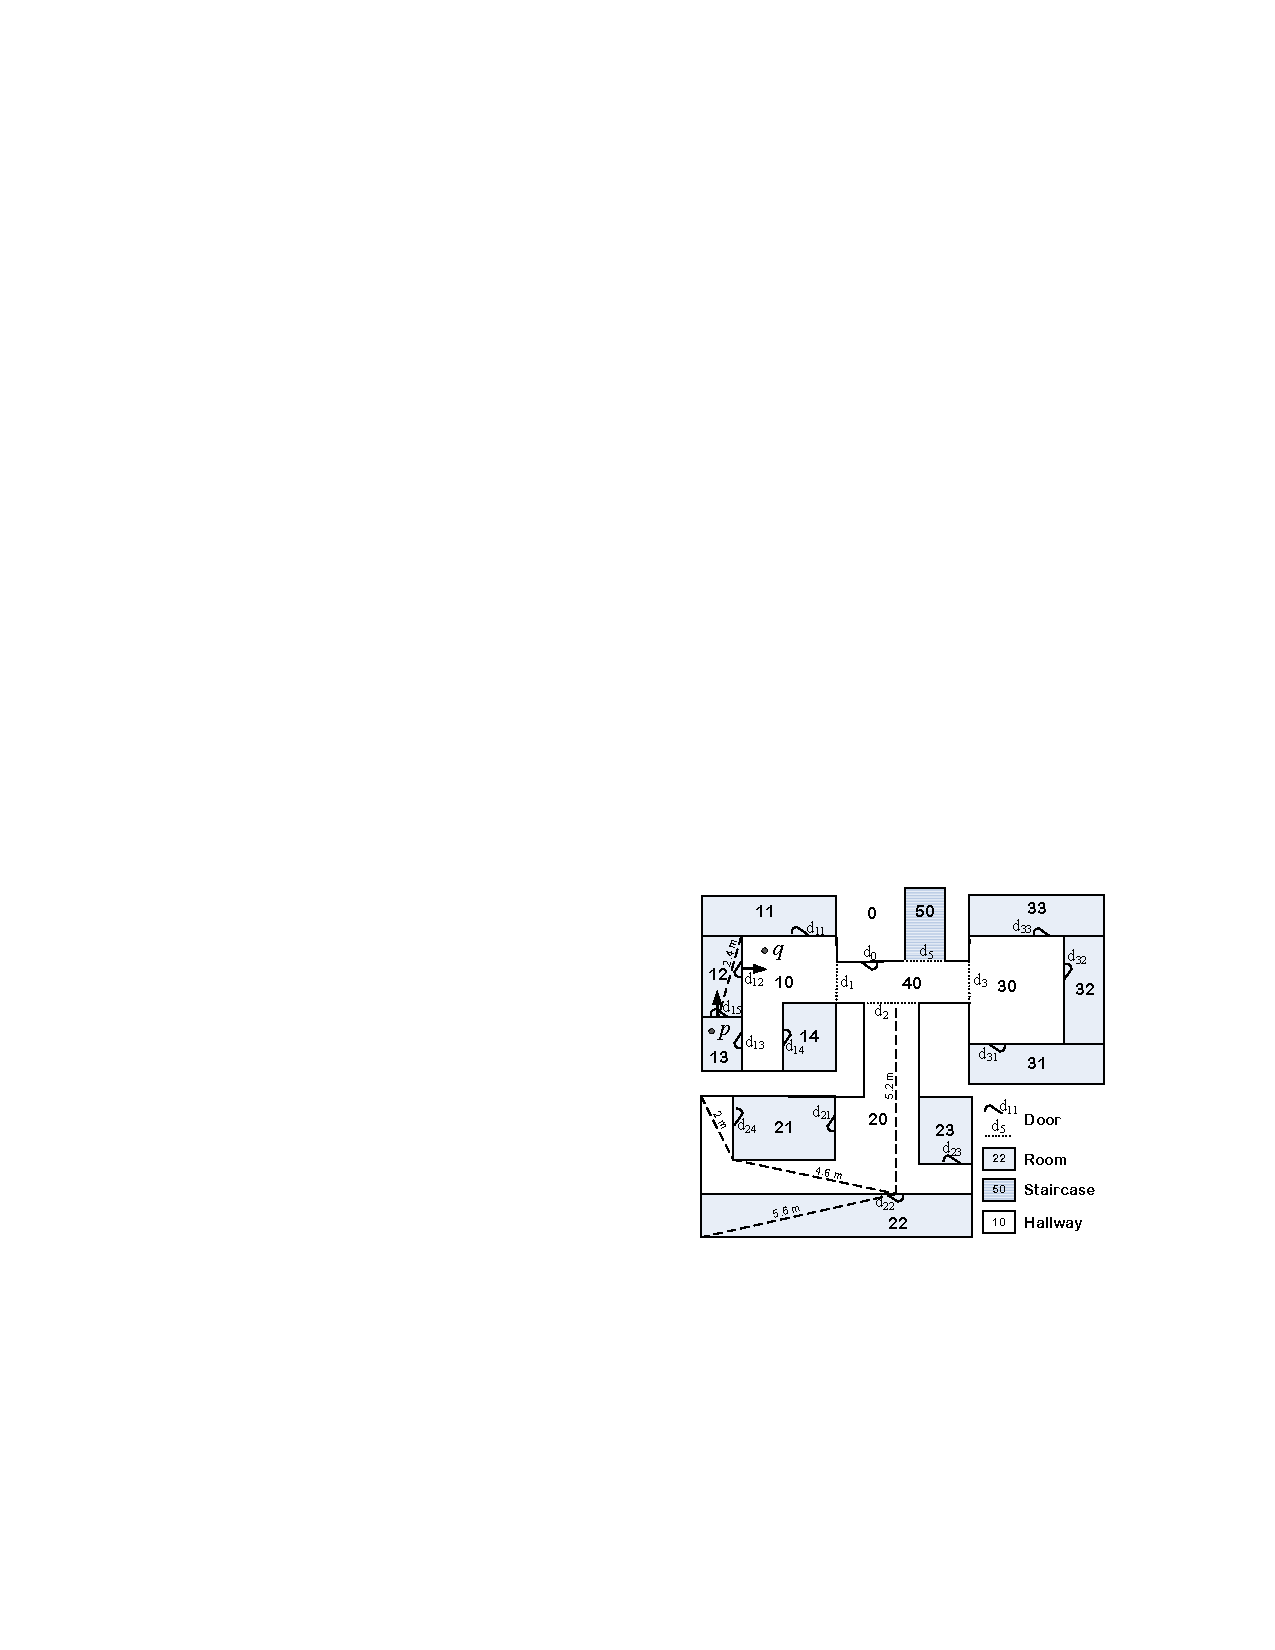
\includegraphics[width=0.85\columnwidth]{figures/2-5/2-5-1.pdf}
  \end{figure}
  \begin{example}
    \textrm{
    \ssize{
      $D2P_{\sqsupset}(d_{12}) = \{ v_{10}\}$, $D2P_{\sqsubset}(d_{12}) = \{ v_{12}\}$
      $P2D_{\sqsupset}(v_{13}) = \{ d_{13}\}$, $P2D_{\sqsubset}(v_{13}) = \{ d_{13}, d_{15}\}$
    }
    }
  \end{example}

  \column{0.48\textwidth}
  \vspace{-15pt}
  \begin{figure}[tb]
    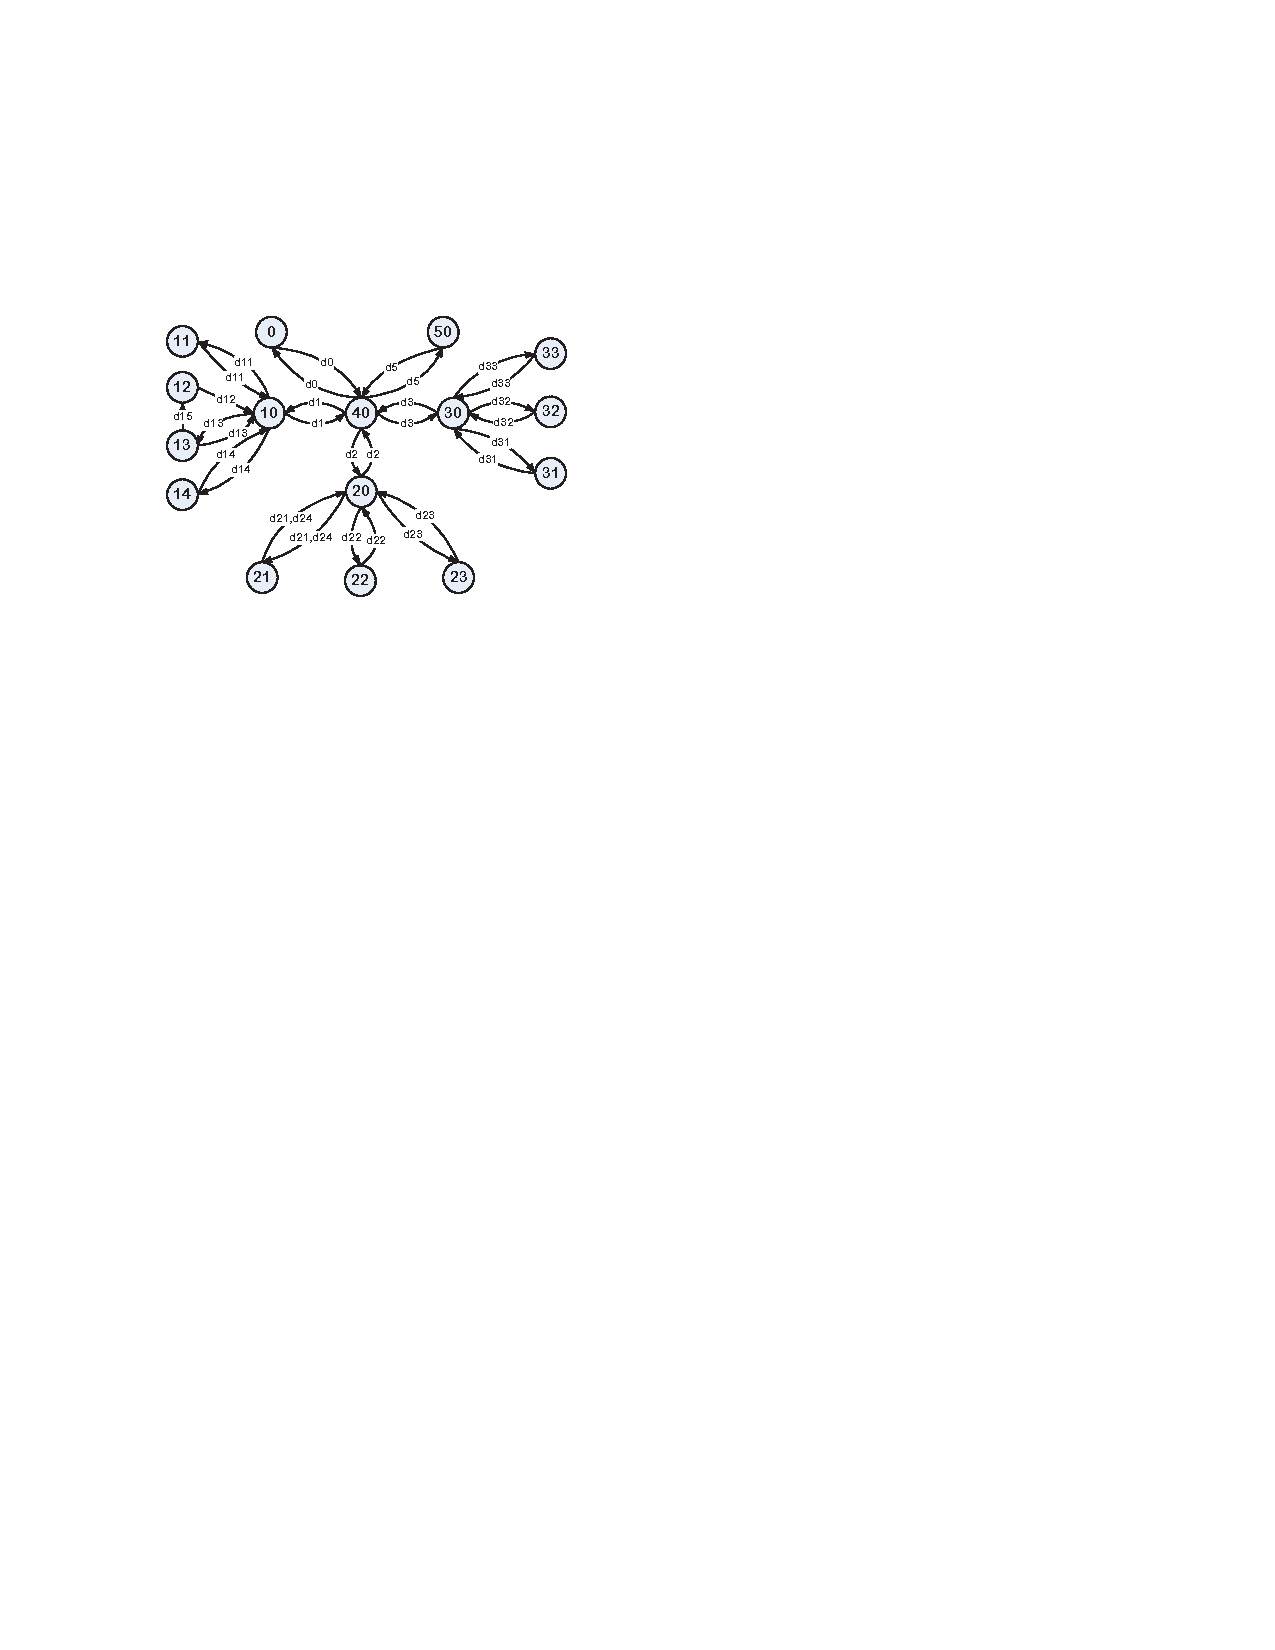
\includegraphics[width=0.8\columnwidth]{figures/2-5/2-5-2.pdf}
  \end{figure}
  \vspace{-10pt}
  \begin{block}{Accessibility Base Graph}
    \textrm{
    \ssize{
    \begin{itemize}
      \item $G_{accs} = \{V, E_a, L\}$
      \item $V = \mathcal{S}_{partition}$ is the set of vertices
      \item $E_a = \{ (v_i, v_j, d_k) | (v_i, v_j) \in D2P(d_k) \}$ is the set of labeled, directed edges
      \item $L = \mathcal{S}_{door}$ is the set of edge labels
    \end{itemize}
    }
    }
  \end{block}

\end{columns}

\end{frame}

%------------------------------------------------

\begin{frame}
\frametitle{Distance-Aware Model}

\fsize{\textrm{The $G_{accs}$ graph does not capture indoor distance information. \conceptbf{Extended Graph Model} is proposed to integrate indoor distances into the graph in a seamless way. \emph{Minimum Indoor Walking Distance}(MIWD) is used. }}

\begin{block}{Extended Graph Model $G_{dist} = \{ V, E_a, L, f_{dv}, f_{d2d} \}$}
  \textrm{
  \begin{sitemize}
    \item $V = \mathcal{S}_{partition}$ is the set of vertices
    \item $E_a = G_{accs}.E_a$
    \item $L = \mathcal{S}_{door}$ is the set of edge labels
    \item $f_{dv} = \mathcal{S} \times V \rightarrow \mathcal{R} \cup \{ \infty \}$ maps an edge to a distance value.
    \begin{equation*}
      f_{dv} = \left\{\begin{matrix}
                \max_{p \in v_j}|| d_i, p || , & if~~ v_j \in D2P_{\sqsupset};
                \\
                \infty , & otherwise.
                \end{matrix}\right.
    \end{equation*}
    \item $f_{d2d} = V \times \mathcal{S}_{door} \times \mathcal{S}_{door} \rightarrow \mathcal{R} \cup \{ \infty \}$ maps a 3-tuple to a distance value.
    \begin{equation*}
      f_{dv} = \left\{\begin{matrix}
                || d_i, d_j ||_{v_k} , & if~~ d_i \in P2D_{\sqsupset}(v_k) and d_j \in P2D_{\sqsubset}(v_k);
                \\
                \infty , & if~~ d_i = d_j and d_i,d_j \in P2D(v_k);
                \\
                0 , & otherwise.
                \end{matrix}\right.
    \end{equation*}
  \end{sitemize}
  }
\end{block}

\end{frame}

%------------------------------------------------

\begin{frame}
\frametitle{Indoor Distance Computation: \emph{door-to-door distance}}

\begin{columns}[c]

  \column{0.52\textwidth}
  \begin{figure}[tb]
    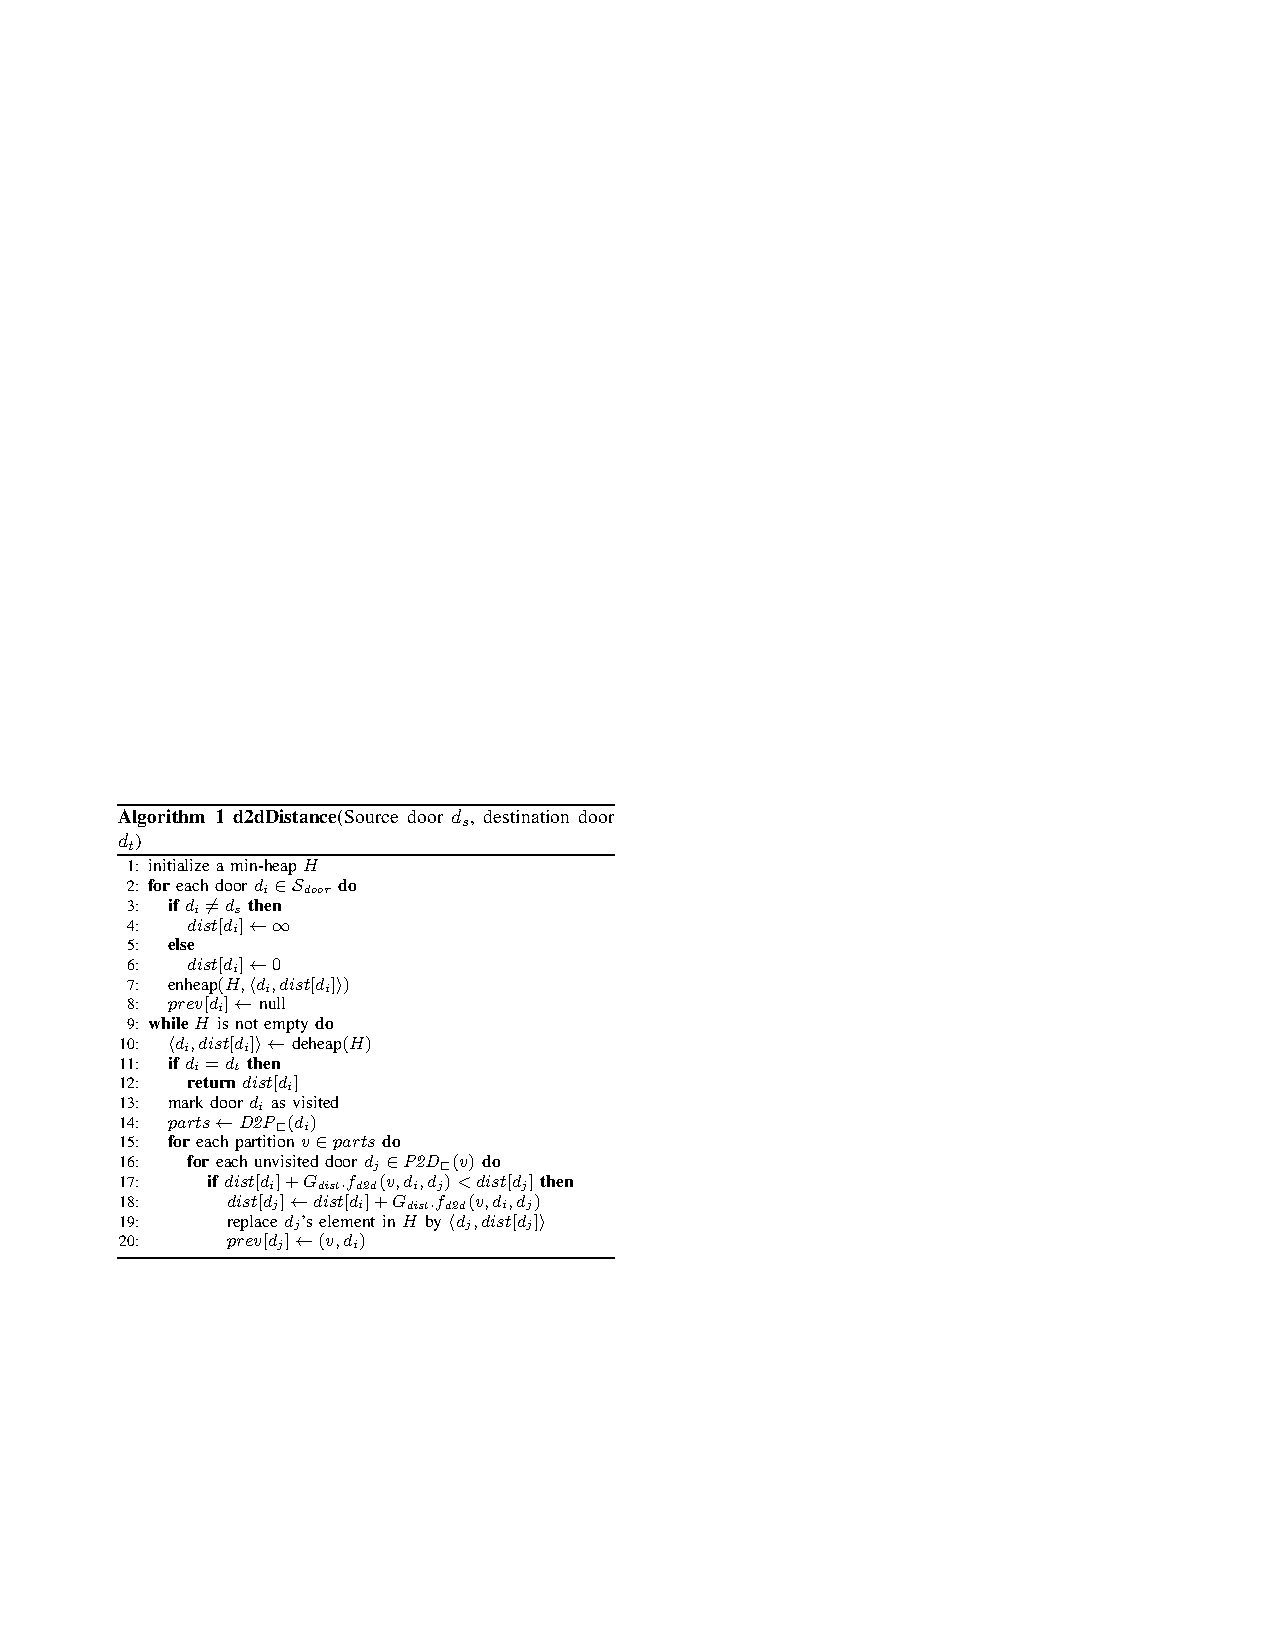
\includegraphics[width=\columnwidth]{figures/2-5/2-5-3.pdf}
  \end{figure}

  \column{0.48\textwidth}


\end{columns}

\end{frame}

%------------------------------------------------

\begin{frame}
\frametitle{Indoor Distance Computation: \emph{point-to-point distance}}

\begin{columns}[c]

  \column{0.52\textwidth}
  \begin{figure}[tb]
    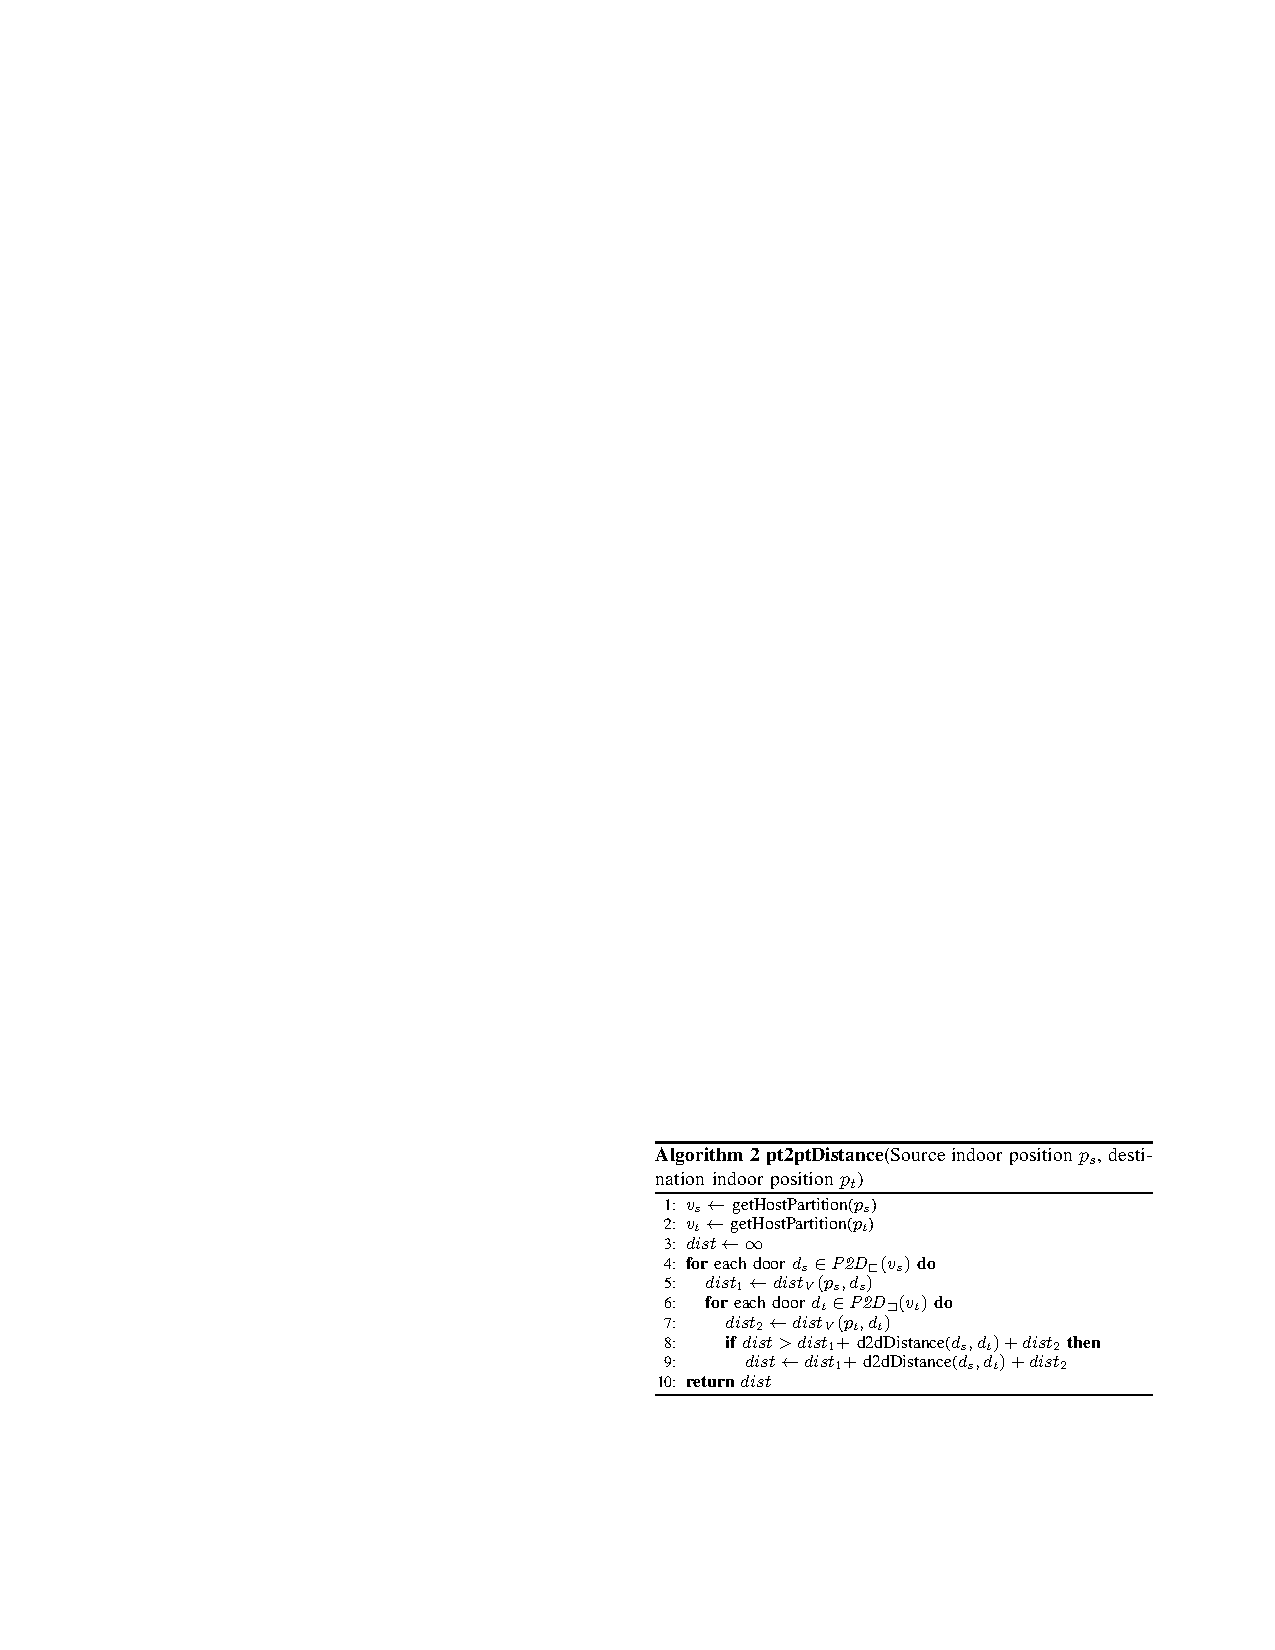
\includegraphics[width=\columnwidth]{figures/2-5/2-5-4.pdf}
  \end{figure}

  \column{0.48\textwidth}


\end{columns}

\end{frame}

%------------------------------------------------

\begin{frame}
\frametitle{Indoor Distance Computation: \emph{point-to-point distance} (I)}

\begin{columns}[c]

  \column{0.52\textwidth}
  \begin{figure}[tb]
    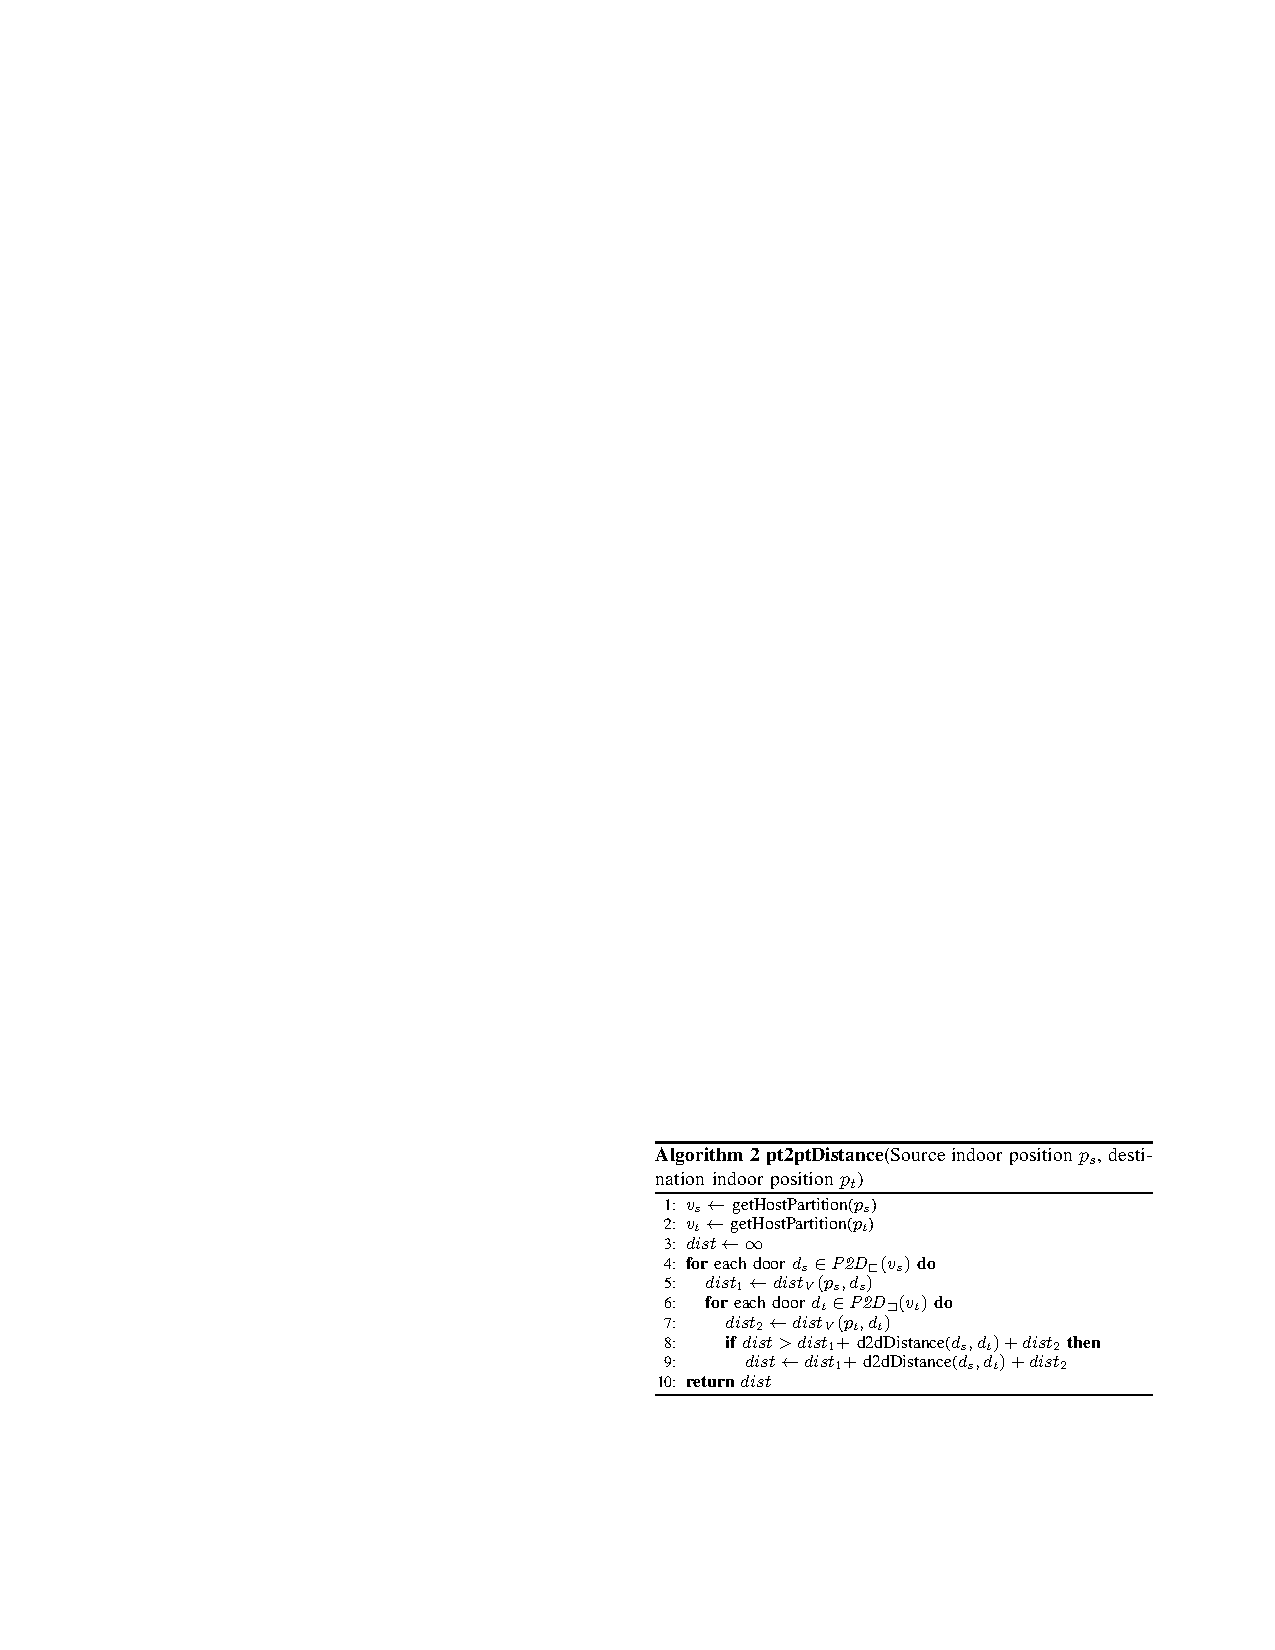
\includegraphics[width=\columnwidth]{figures/2-5/2-5-4.pdf}
  \end{figure}

  \column{0.48\textwidth}


\end{columns}

\end{frame}

%------------------------------------------------

\begin{frame}
\frametitle{Indoor Distance Computation: \emph{point-to-point distance} (II)}

\begin{columns}[c]

  \column{0.4\textwidth}
  \begin{figure}[tb]
    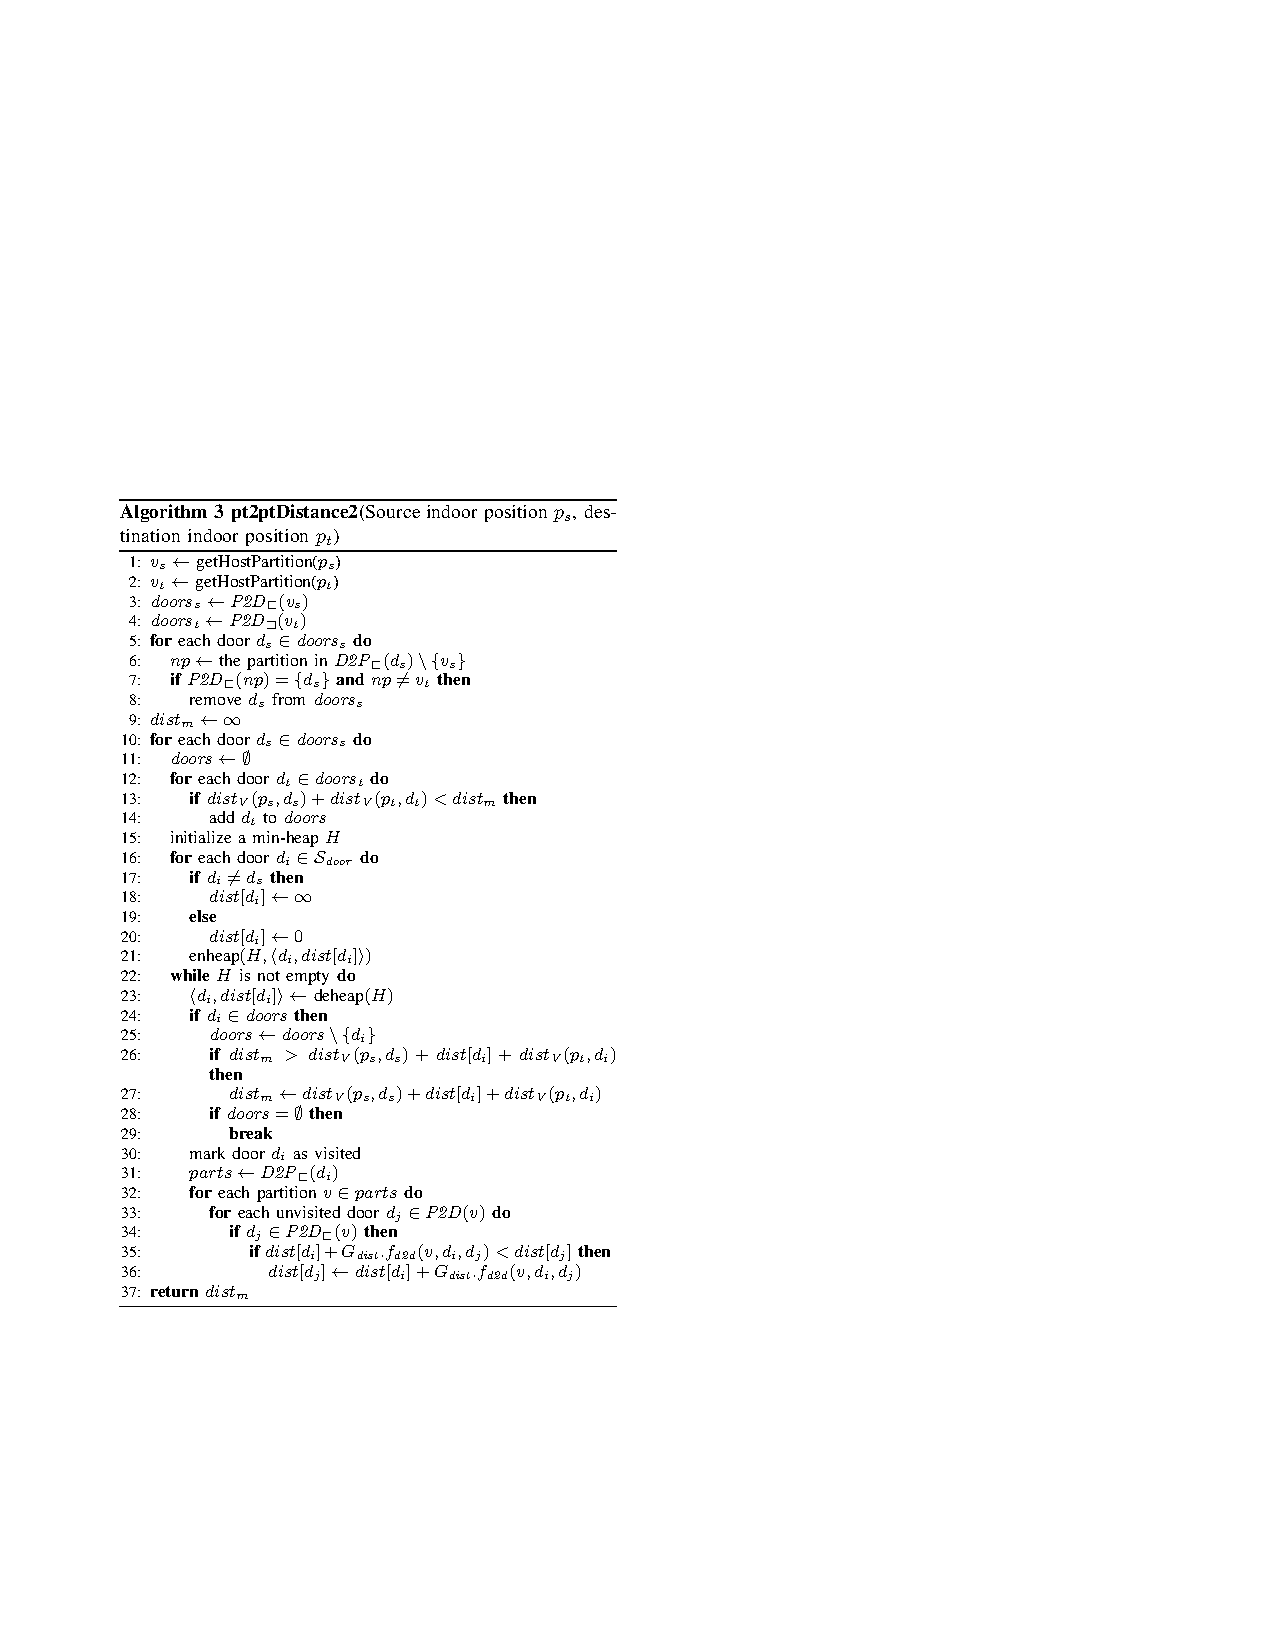
\includegraphics[width=\columnwidth]{figures/2-5/2-5-5.pdf}
  \end{figure}

  \column{0.48\textwidth}


\end{columns}

\end{frame}


% %------------------------------------------------
%
% \begin{frame}
% \frametitle{Indoor Distance Computation: \emph{point-to-point distance} (III)}
%
% \begin{columns}[c]
%
%   \column{0.52\textwidth}
%   \begin{figure}[tb]
%     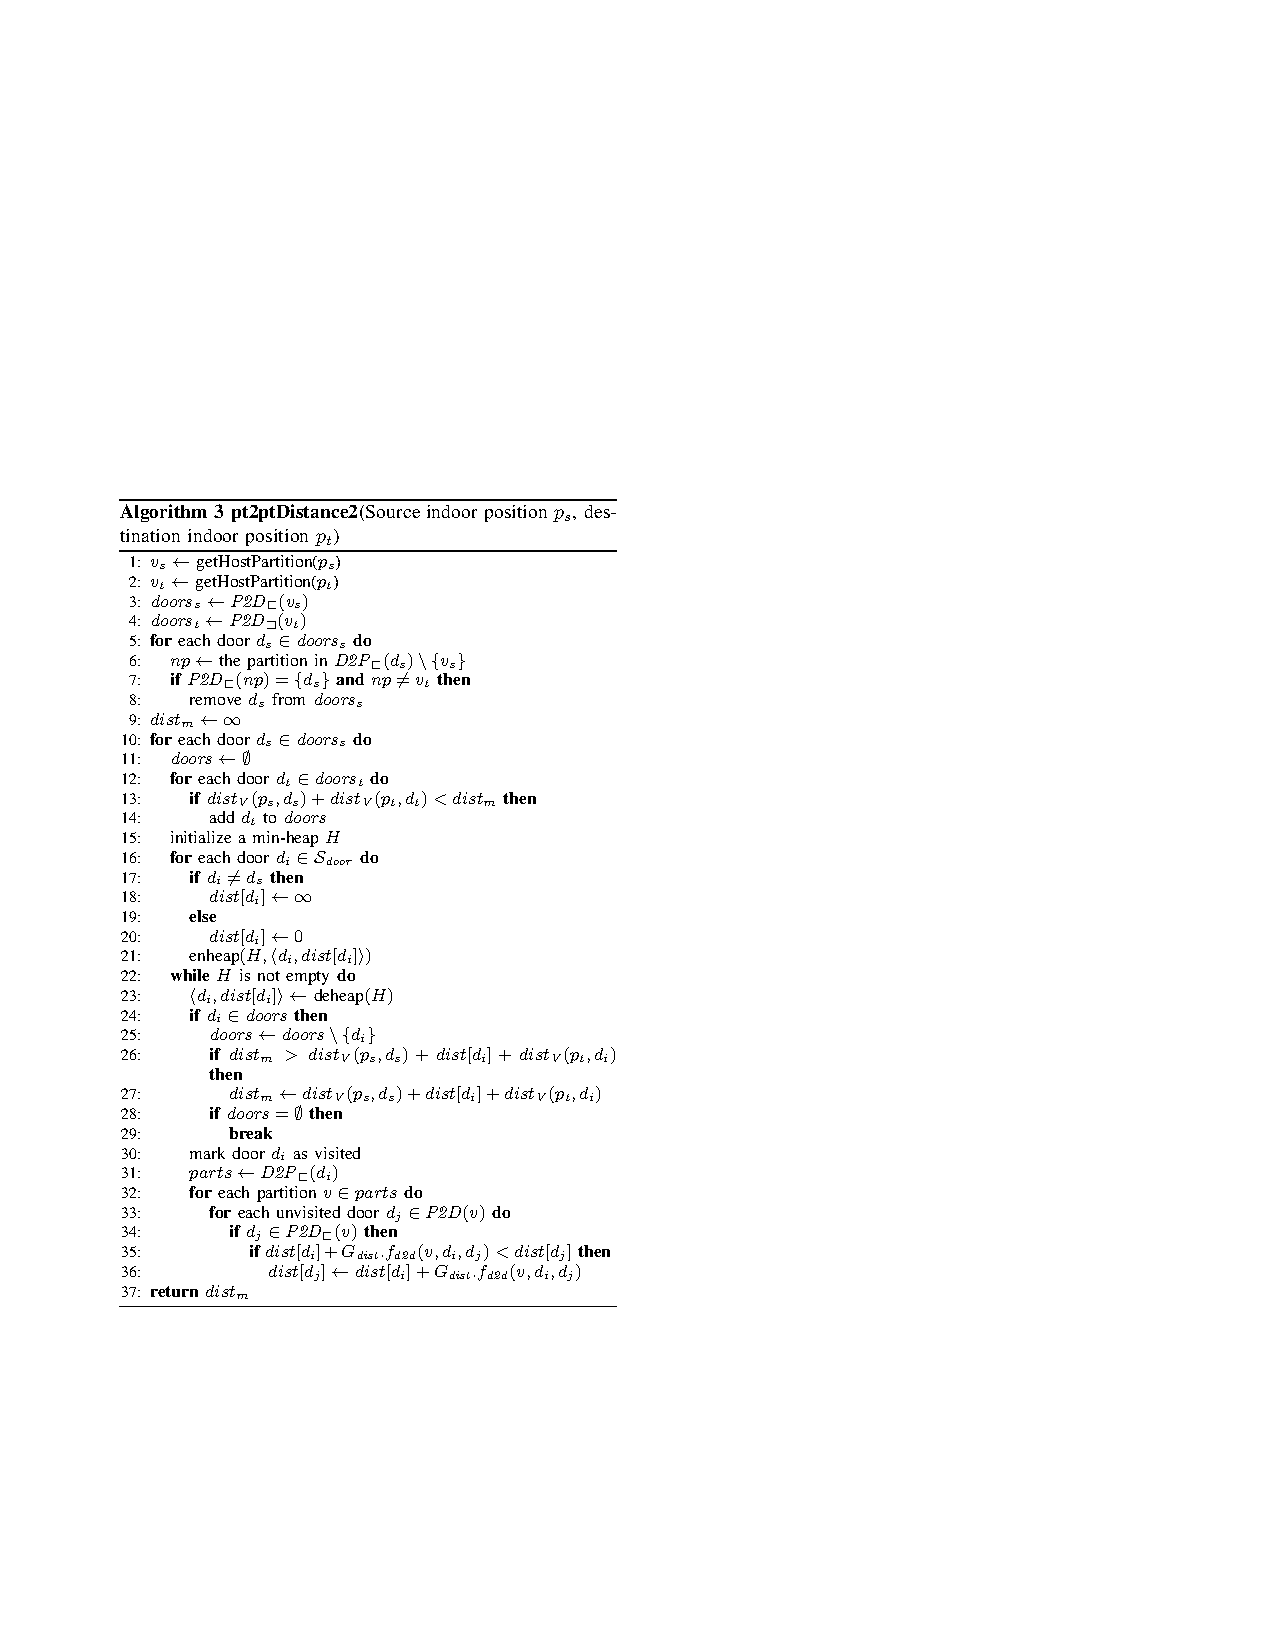
\includegraphics[width=\columnwidth]{figures/2-5/2-5-5.pdf}
%   \end{figure}
%
%   \column{0.48\textwidth}
%
%
% \end{columns}
%
% \end{frame}

% %------------------------------------------------

\begin{frame}[allowframebreaks]
\frametitle{References}

\begin{thebibliography}{99} % Beamer does not support BibTeX so references must be inserted manually as below
\bibliographystyle{abbrv}
\fsize{

\bibitem{DBLP:conf/mdm/JensenLY09}
C.~S. Jensen, H.~Lu, and B.~Yang.
\newblock Graph model based indoor tracking.
\newblock In {\em {MDM}}, pp. 122--131, 2009.

\bibitem{DBLP:conf/cikm/YangLJ09}
B.~Yang, H.~Lu, and C.~S. Jensen.
\newblock Scalable continuous range monitoring of moving objects in symbolic
  indoor space.
\newblock In {\em CIKM}, pp. 671--680, 2009.

\bibitem{DBLP:conf/edbt/YangLJ10}
B.~Yang, H.~Lu, and C.~S. Jensen.
\newblock Probabilistic threshold k nearest neighbor queries over moving
  objects in symbolic indoor space.
\newblock In {\em EDBT}, pp. 335--346, 2010.

\bibitem{DBLP:conf/icde/LuYCJ11}
H.~Lu, B.~Yang, and C.~S. Jensen.
\newblock Spatio-temporal Joins on Symbolic Indoor Tracking Data.
\newblock In {\em {ICDE}}, pp. 816--827, 2011.

\bibitem{jensen2010indoor}
C.~S. Jensen, H.~Lu and B.~Yang.
\newblock Indoor-A New Data Management Frontier.
\newblock In {\em IEEE Data Eng. Bull.}, pp. 12--17, 2010.

\bibitem{DBLP:conf/icde/LuCJ12}
H.~Lu, X.~Cao, and C.~S. Jensen.
\newblock A foundation for efficient indoor distance-aware query processing.
\newblock In {\em ICDE}, pp. 438--449, 2012.

\bibitem{becker2005location}
C.~Becker and F.~D{\"u}rr.
\newblock On location models for ubiquitous computing.
\newblock In {\em Personal and Ubiquitous Computing}, pp. 20--31, 2005.

\bibitem{li2008lattice}
D.~Li and D.~L.~Lee.
\newblock A lattice-based semantic location model for indoor navigation.
\newblock In {\em MDM}, pp. 17--24, 2008.

\bibitem{becker2009multilayered}
T.~Becker, C.~Nagel and T.~H.~Kolbe
\newblock A multilayered space-event model for navigation in indoor spaces.
\newblock In {\em 3D Geo-Information Sciences}, pp. 61--77, 2009.

}
\end{thebibliography}

\end{frame}


\subsection{2.6 Efficient Distance-aware Query Evaluation on Indoor Moving Objects} % A subsection can be created just before a set of slides with a common theme to further break down your presentation into chunks

% \begin{frame}
\frametitle{About This Work...}

\emph{Efficient Distance-Aware Query Evaluation on Indoor Moving Objects}.~\cite{DBLP:conf/icde/XieLP13} \\
X.~Xie, H.~Lu, and T.~B. Pedersen.\\~\\

\begin{itemize}
  \item Published at \emph{ICDE' 2013}.
  \item Study indoor distances and effective prunning bounds in relation to indoor moving objects.
  \item Design a composite index for indoor spaces and moving objects.
  \item Define and evaluate range queries as well as $k$nn queries on indoor moving objects.
\end{itemize}

\end{frame}

%------------------------------------------------

\begin{frame}
\frametitle{Motivation}

\begin{itemize}
  \item In many indoor LBS scenarios, appropriate handling of indoor distances and relevant queries is of critical.
    \begin{fitemize}
      \item a cafe in a mall may send message to nearby shoppers to boost its business
      \item in a large airport, it important to minitor individuals within a pre-defined range from a sensitive point
    \end{fitemize}

  \item Indoor spaces are characterized by many special entities and thus render distance calculation very complex.

  \item The limitations of indoor positioning technologies create inherent uncertainties in indoor moving objects data.

\end{itemize}

\end{frame}

%------------------------------------------------

\begin{frame}
\frametitle{Notations}

\begin{figure}[tb]
  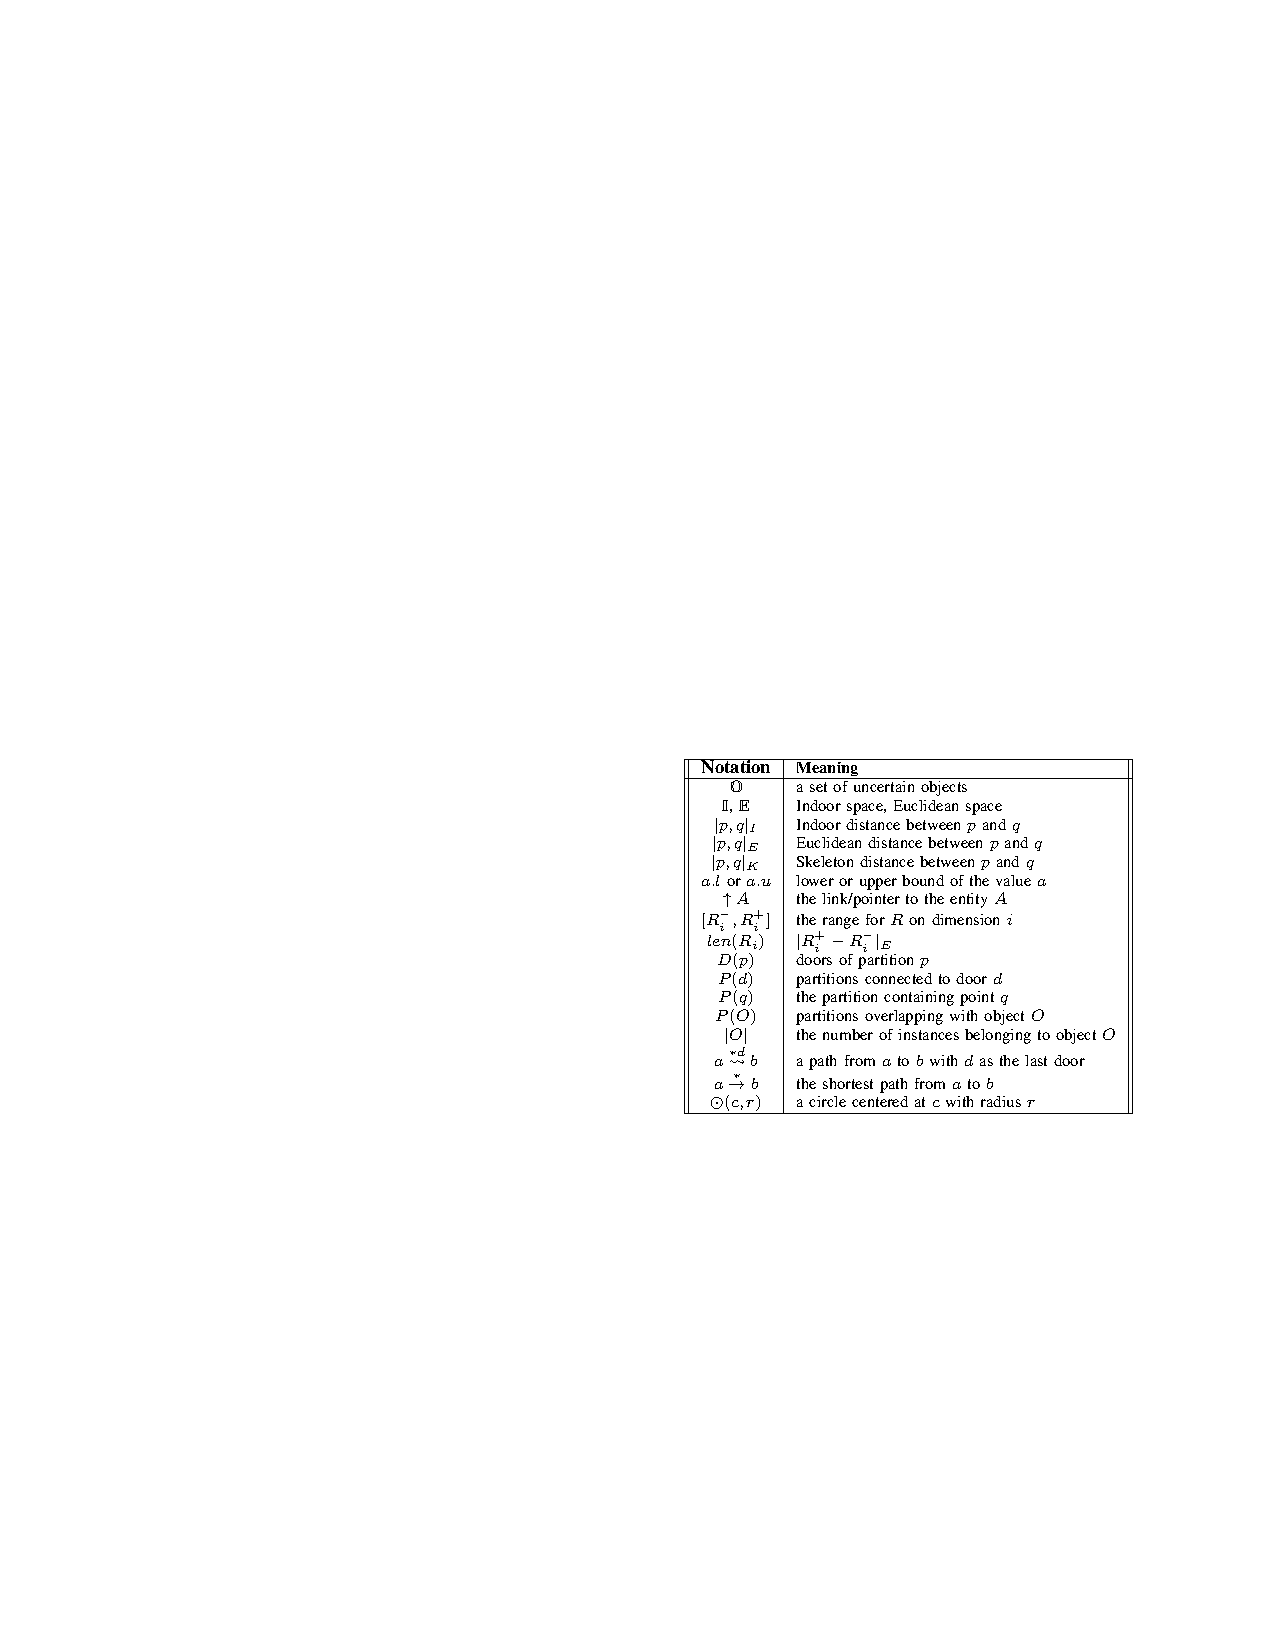
\includegraphics[width=0.75\columnwidth]{figures/2-6/2-6-1.pdf}
\end{figure}

\end{frame}

%------------------------------------------------

\begin{frame}
\frametitle{Preliminaries: Indoor Space and Indoor Distance}

\conceptbf{Doors Graph} has been proposed to represent the connectivity of indoor partitions as well as door-to-door distances.~\cite{DBLP:conf/edbt/YangLJ10}\\~\\\pause

Given two indoor positions $p$ an $q$, we use $q \overset{\delta}{\rightsquigarrow} p$ to denote a path from $q$ to $p$ where $\delta$ is the sequence of doors on the path.\\~\\\pause

The length of the shortest path as \emph{indoor distance} from $q$ to $p$, and denote it formally as $|q, p|_{I} = min_{\delta}(|q \overset{\delta}{\rightsquigarrow} p|)$, also $q \overset{\delta}{\rightarrow} p$.\\~\\\pause

\emph{indoor distance} consists of \emph{door-door distance} and \emph{intra-partition object-door distance}:\pause
\begin{equation}
  min_{d_q \in D(q), d_p \in D(p)}(|q, d_q|_{E} + |d_q, d_p|_{I} + |d_p, p|_{E})
\end{equation}

\end{frame}

%------------------------------------------------

\begin{frame}
\frametitle{Indoor Moving Objects}

\begin{itemize}
  \item Existing proposals~\cite{pfoser1999capturing, DBLP:conf/edbt/YangLJ10} model a moving object by an \emph{uncertainty region}, where the exact location is considered as a random variable inside.
  \item The possibility of its appearance can be collected by object's velocities~\cite{DBLP:conf/edbt/YangLJ10}, parameters of positioning device~\cite{pfoser1999capturing}, or analysis of historical records (represented by \emph{pdf}).
  \item The \emph{pdf} can be either a close form equation~\cite{cheng2003evaluating,cheng2004querying} or a set of instance representation~\cite{kriegel2007probabilistic}, as it is general for arbitrary distribution.
  \item Thus, an indoor moving object $O$ is represented by a set ${(s_i, p_i)}$, where $s_i$ is an instance and $p_i$ is its \emph{existential probability}, satisfying $\sum_{s_i \in O}p_i = 1$.
\end{itemize}

\end{frame}

%------------------------------------------------

\begin{frame}
\frametitle{Expected Indoor Distance}

\begin{definition}[Expected Indoor Distance for Uncertain Object]
  Given a fixed point $q \in \mathbb{I}$ and an uncertain object $O$, the indoor distance from $q$ to $O$ is
  \begin{equation}
    |q, O|_{I} = E_{s_i \in O}(|q,s_i|_{I}) = \sum_{s_i \in O}|q,s_i|_{I} \cdot p_i
  \end{equation}
\end{definition}
\vspace{10pt}
an object $O$'s uncertainty region may overlap with multiple partitions. Accordingly, all the instances in $O$ are divided into subsets, i.e., $O = \cup_{1 \leq j \leq m}S[j](1 \leq m \leq |O|)$ where each $S[j]$ corresponds to a different partition, it is called $O$'s \emph{uncertainty subregion}.

\end{frame}

%------------------------------------------------

\begin{frame}
\frametitle{Case of Indoor Distance $|q, O|_I$ (I)}

\conceptbf{Single-Partition Single-Path Distance}~$O$'s uncertainty region falls into one single partition $P$. For an arbitrary $s_i \in O$, the shortest path $q \overset{*d}{\rightarrow} s_i$ shares the path enters $P$ to reach $s_i$.

\begin{equation}
  |q, O|_{I} = |q,d|_I + \sum_{s_i \in O}|d, s_i|_E \cdot p_i
\end{equation}

\end{frame}

%------------------------------------------------

\begin{frame}
\frametitle{Case of Indoor Distance $|q, O|_I$ (II)}

\conceptbf{Single-Partition Multi-Path Distance}~$O$'s uncertainty region still falls into one single partition $P$. However, for different instances $s_i$ and $s_j$, the shortest path $q \overset{*}{\rightarrow} s_i$ and $q \overset{*}{\rightarrow} s_j$ do not share the same door sequence.

\begin{equation}
  |q, O|_{I} = \sum_{s_i \in O}|q, s_i|_I \cdot p_i
\end{equation}

\begin{columns}[c]

  \column{0.24\textwidth}
  \begin{figure}[tb]
    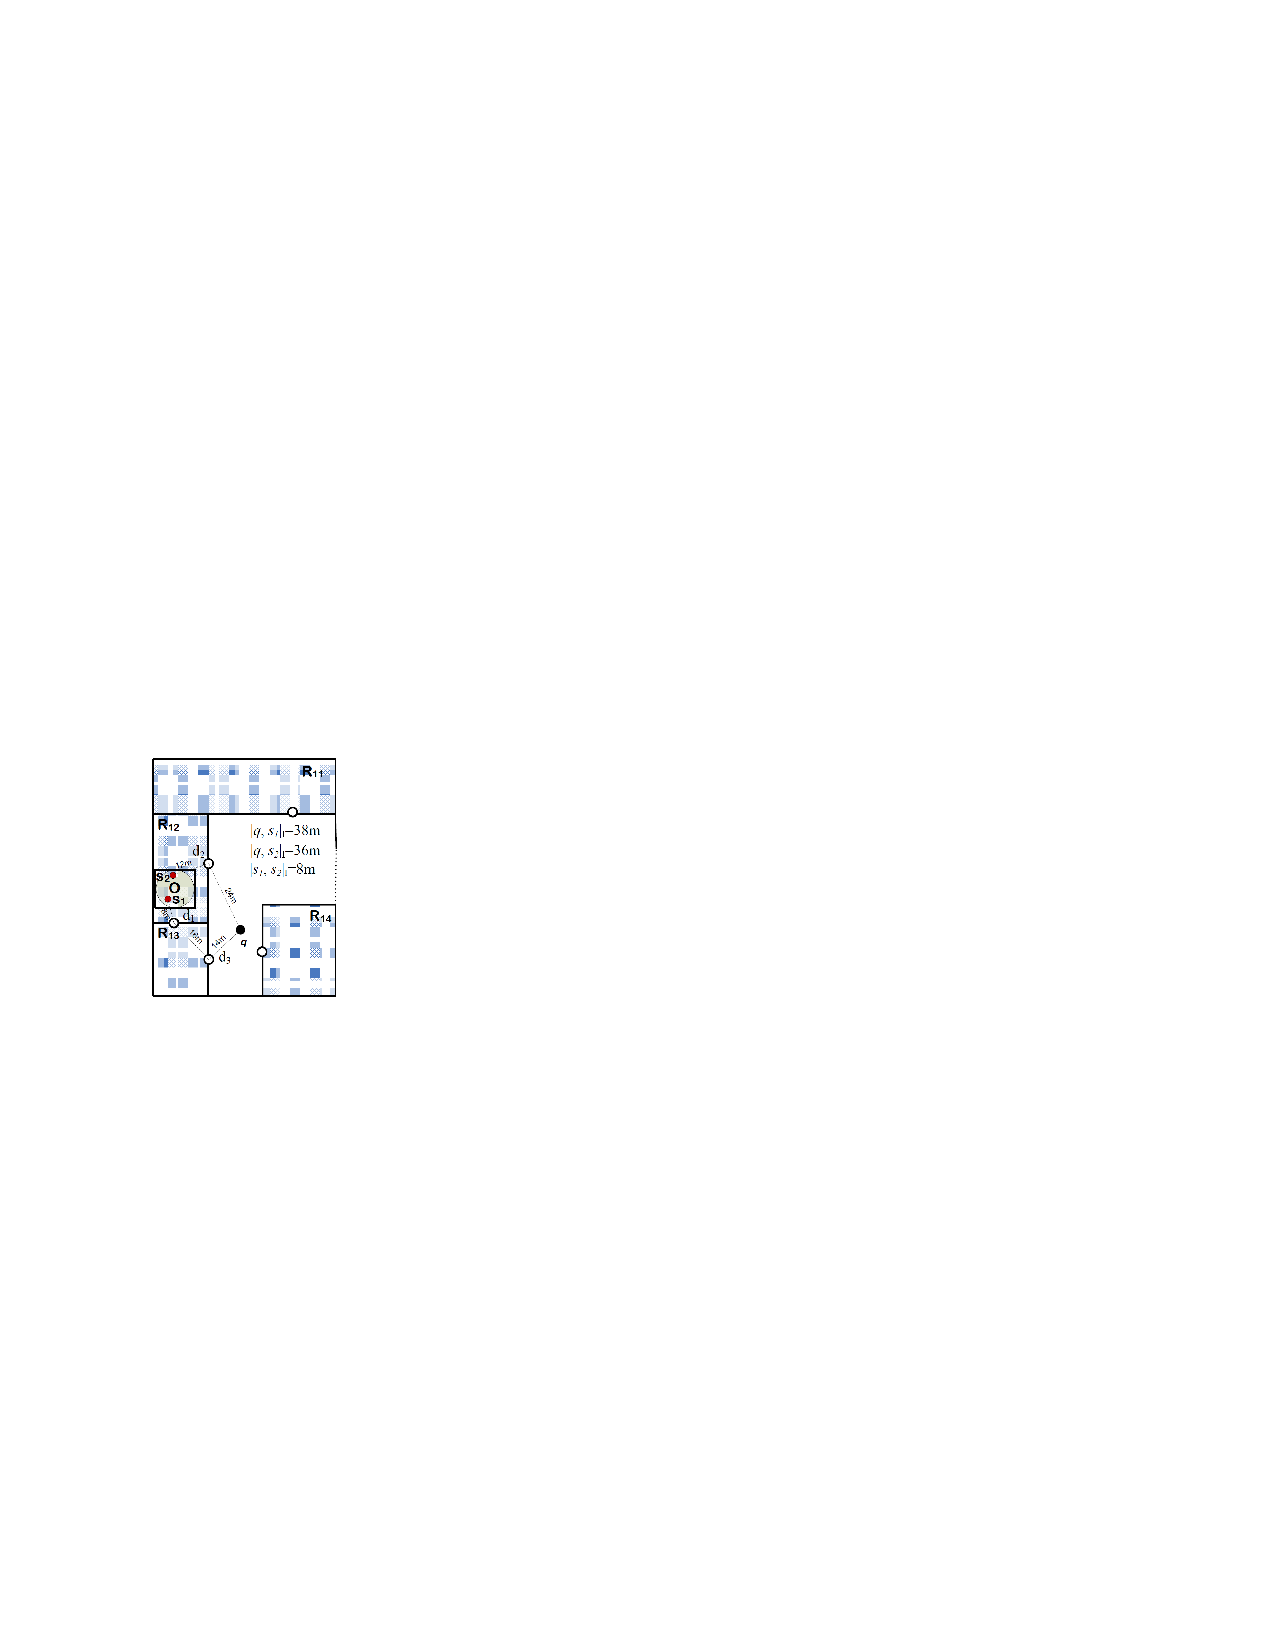
\includegraphics[width=\columnwidth]{figures/2-6/2-6-2.pdf}
  \end{figure}

  \column{0.76\textwidth}
  \begin{example}
    $O$ has two instance $s_1$ and $s_2$, the shortest path from $q$ to them are: $q \overset{d_3, d_1}{\rightsquigarrow} s_1$ and $q \overset{d_2}{\rightsquigarrow} s_2$.
  \end{example}

\end{columns}

\end{frame}

%------------------------------------------------

\begin{frame}
\frametitle{Case of Indoor Distance $|q, O|_I$ (II)}

The \emph{solution space} of the single-partition multi-path distance is the \conceptbf{Additive Weighted Voronoi Diagram}.\\~\\

Suppose partition $P$ has doors $\{d_1, ..., d_m\}$, for each door $d_i$, a weight $w_i = |q, d_i|_I$ is assigned. Use \emph{weighted bisectors} to represent the \emph{Additive Weighted Voronoi Diagram}. Given two doors $d_i$ and $d_j$, whose weights are $w_i$ and $w_j$, respectively, the \emph{weighted bisector} $b_{ij}$ is a curve:
\begin{equation}
  b_{ij} = \{ p : |p,d_i|_E + w_i = |p,d_j|_E + w_j \}
\end{equation}

\vspace{-20pt}
\begin{columns}[c]

  \column{0.2\textwidth}
  \begin{figure}[tb]
    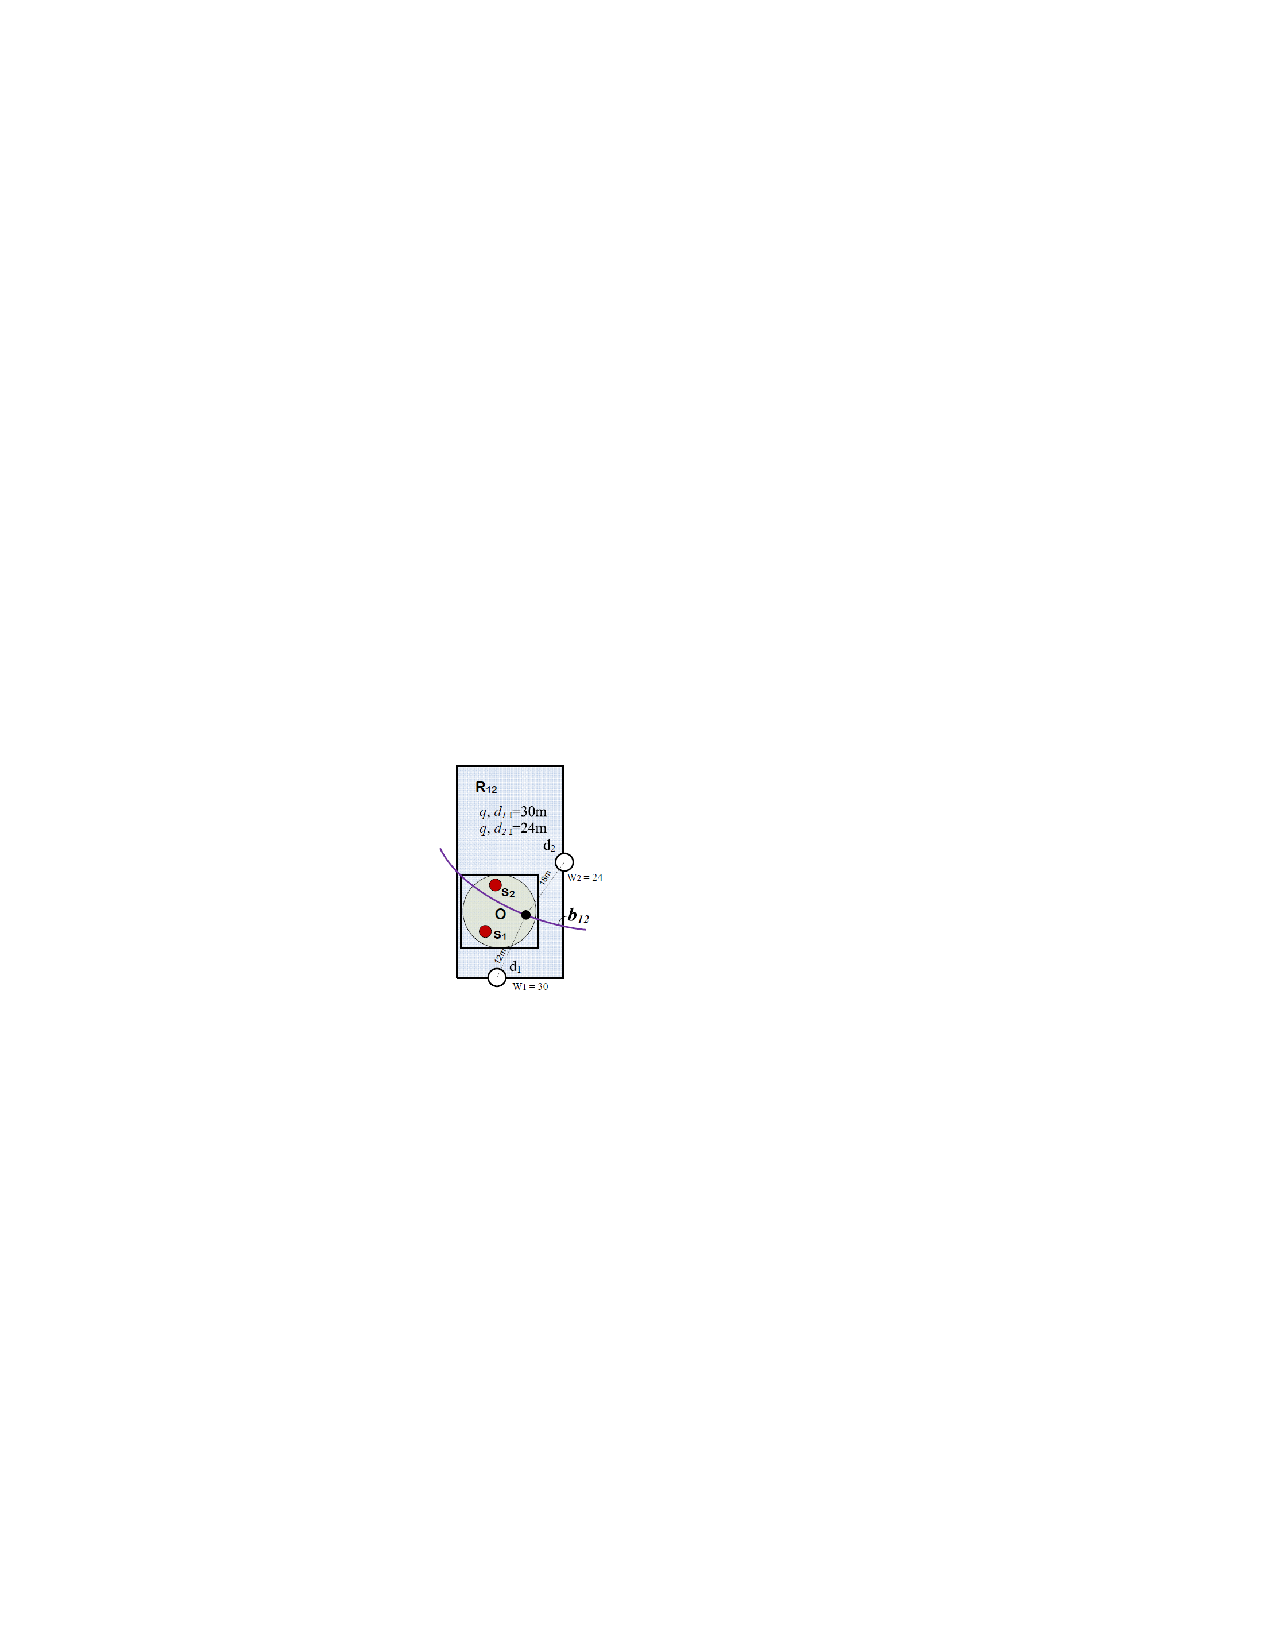
\includegraphics[width=\columnwidth]{figures/2-6/2-6-4.pdf}
  \end{figure}

  \column{0.8\textwidth}
  \begin{figure}[tb]
    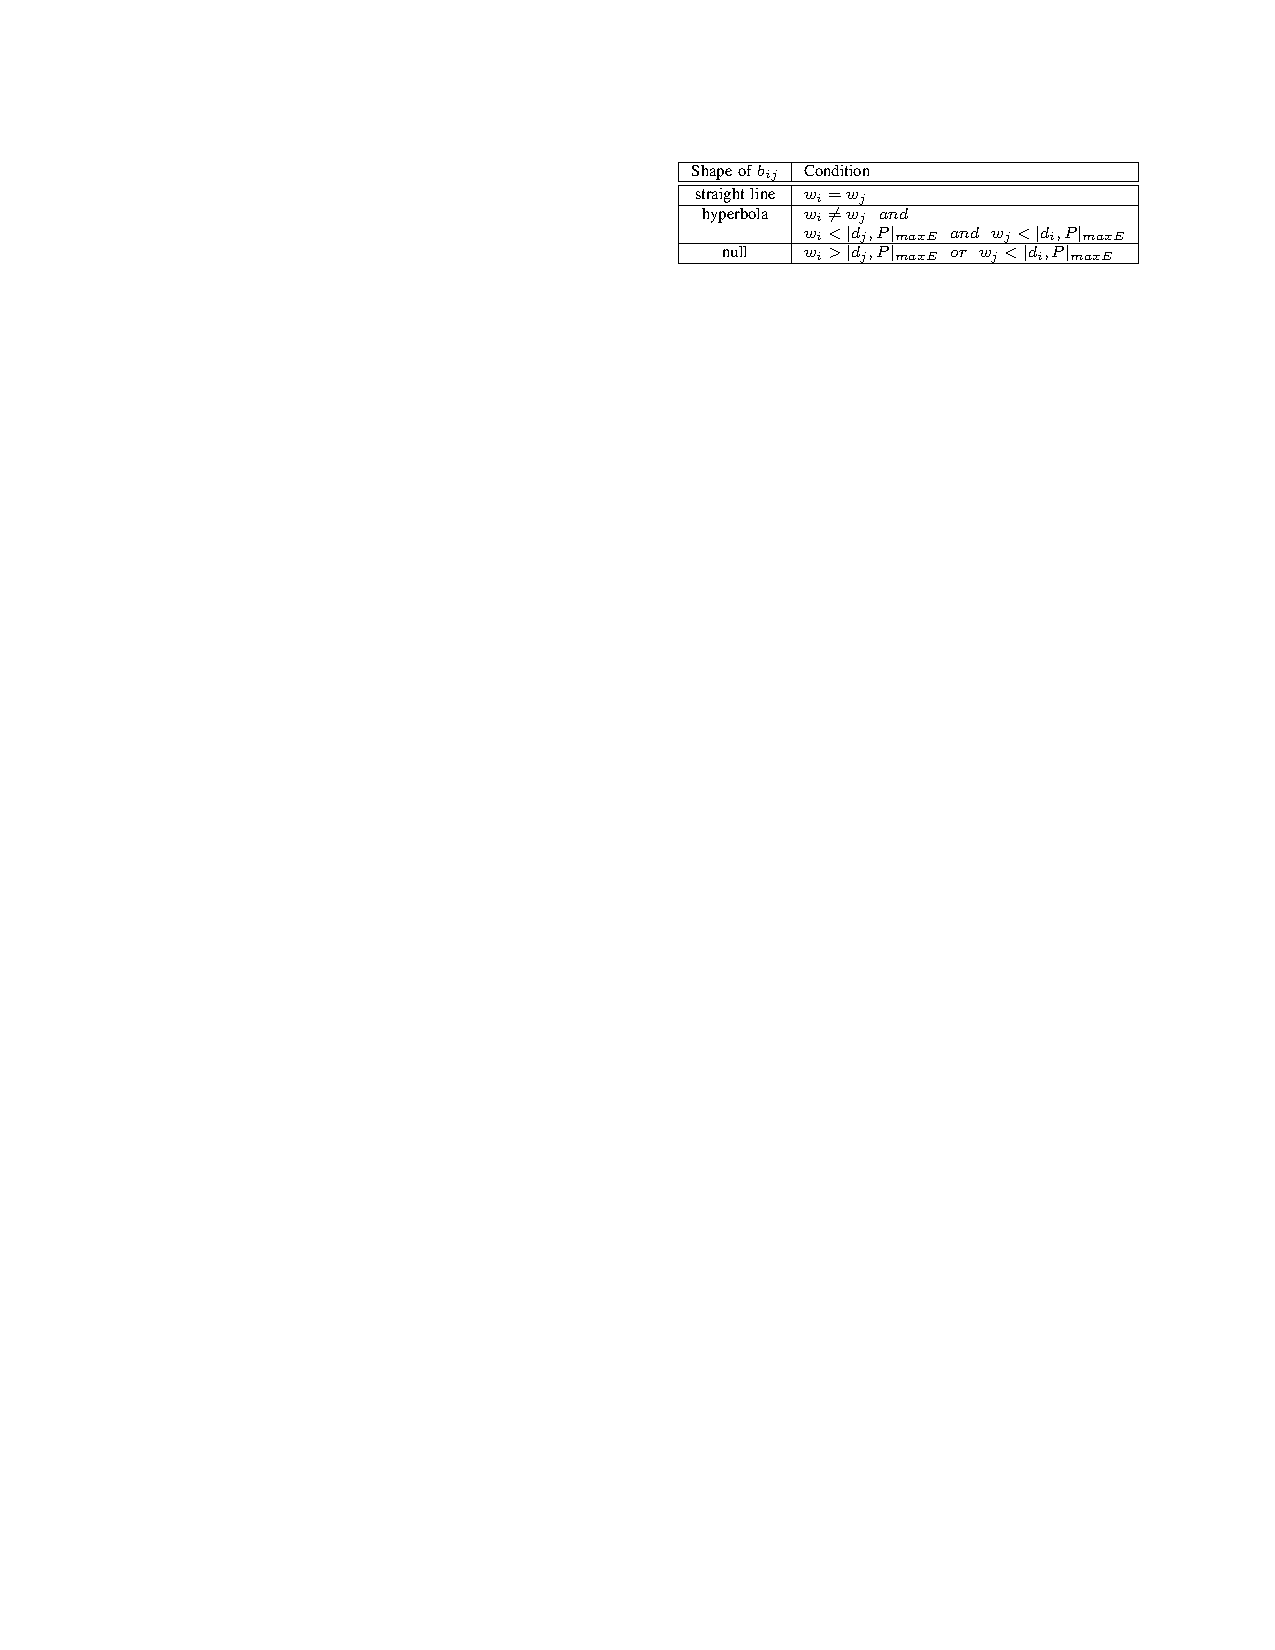
\includegraphics[width=\columnwidth]{figures/2-6/2-6-3.pdf}
  \end{figure}

\end{columns}

\end{frame}

%------------------------------------------------

\begin{frame}
\frametitle{Case of Indoor Distance $|q, O|_I$ (III)}

\conceptbf{Multi-Partition Multi-Path Distance}~$O$'s uncertainty region overlaps with more than one partition, and thus $O = \cup_{1 \leq j \leq m}S[j](1 \leq m \leq |O|)$.

\begin{equation}
  |q, O|_I = \sum_{1 \leq j \leq m}(|q,S[j]|_I \cdot \sum_{s_i \in S[j]}p_i)
\end{equation}

$|q,S[j]|_I$ is calculated according to case I or case II, by substituting $S[j]$ for $O$.

\vspace{-5pt}
\begin{columns}[c]

  \column{0.2\textwidth}
  \begin{figure}[tb]
    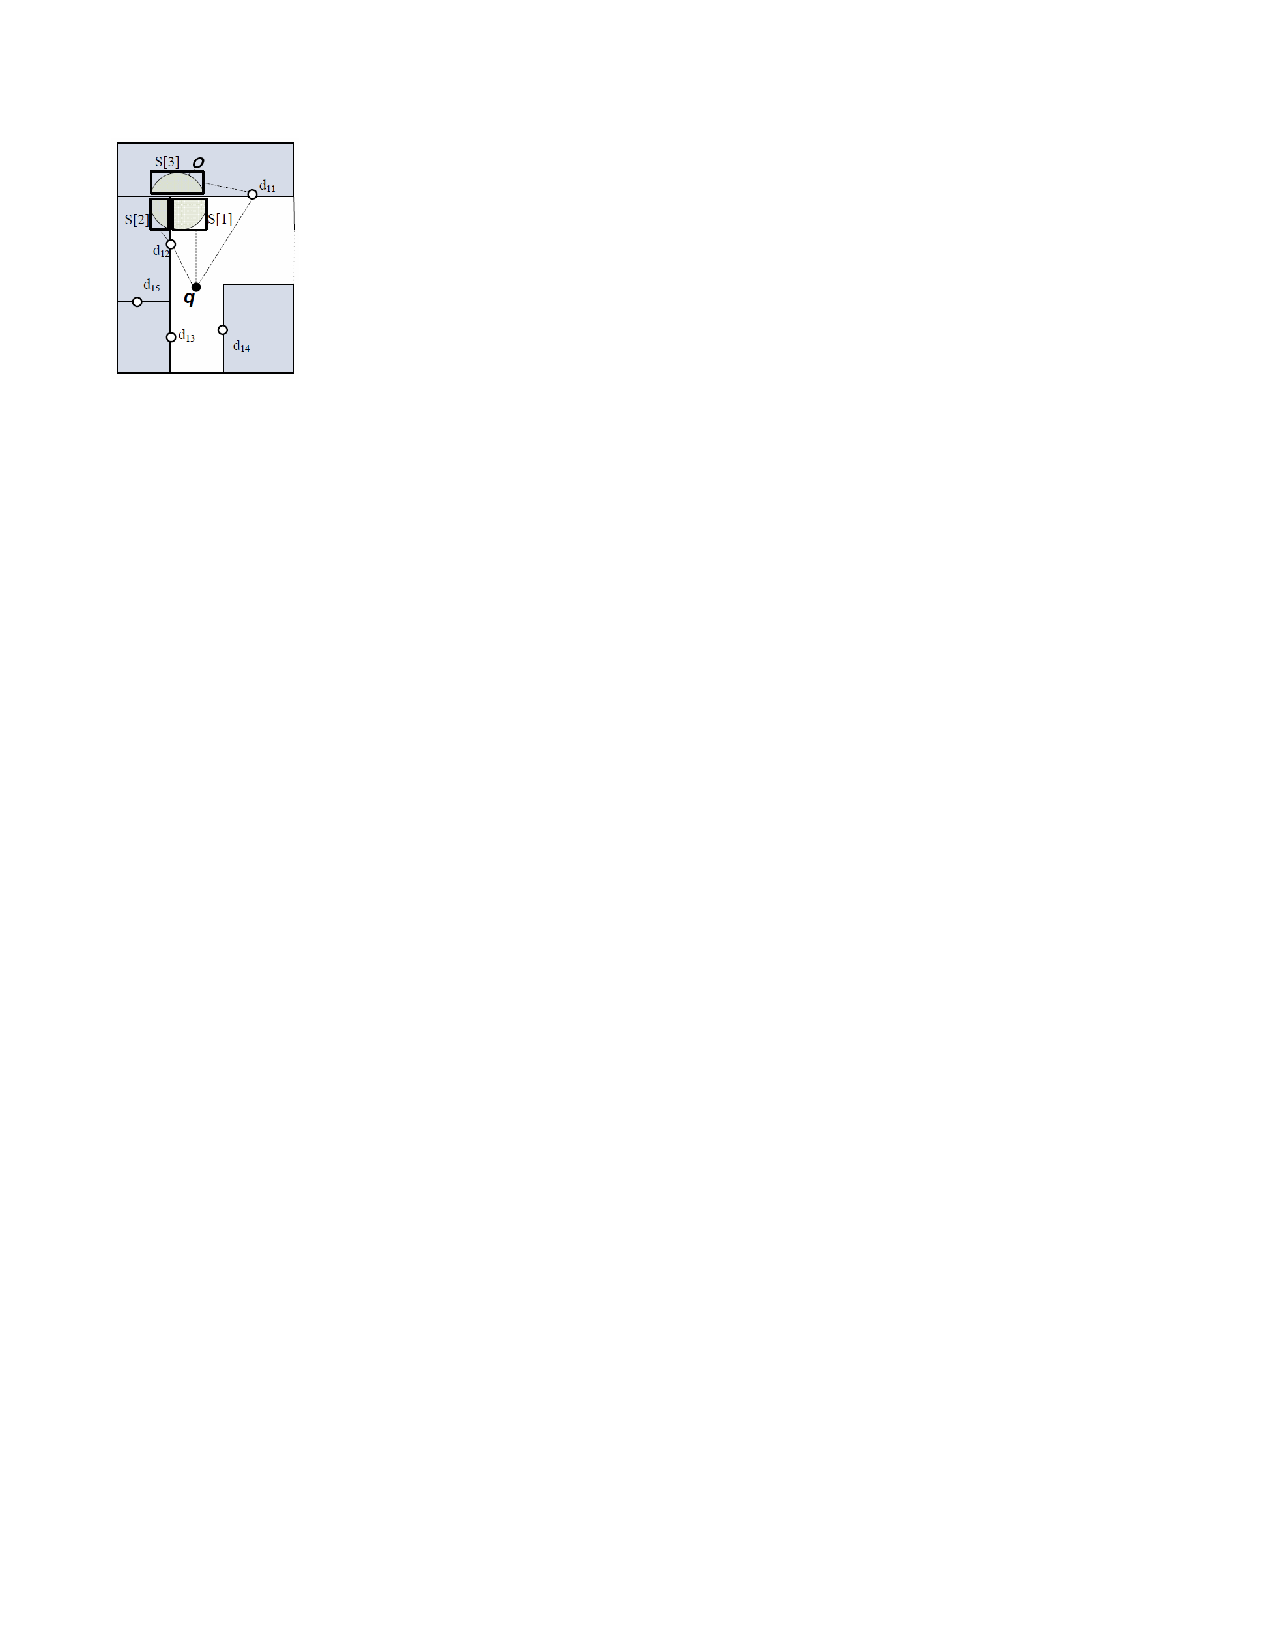
\includegraphics[width=\columnwidth]{figures/2-6/2-6-5.pdf}
  \end{figure}

  \column{0.8\textwidth}
  \begin{example}
    $O$ has three uncertainty subregions $S_1$, $S_2$ and $S_3$. Accordingly, $|q,O|_I = E(\sum_{1 \leq j \leq 3}(|q, S[j]_I|))$.
  \end{example}

\end{columns}

\end{frame}

%------------------------------------------------

\begin{frame}
\frametitle{Bounds for Indoor Distances}

\conceptbf{Euclidean Lower Bounds}

\vspace{10pt}
\begin{lemma}[Euclidean Lower Bounds]
  For point $q$ and object $O$ in an indoor space, the (virtual) Euclidean distance between them is the lower bound of their indoor space. Therefore, it has $|q,O|_{minE} \leq |q,O|_I$, where $|q, O|_{minE} = \min_{s_i \in O}|q,s_i|_E$.
\end{lemma}

\vspace{10pt}
\textrm{it is impossible to derive the indoor upper bounds by using Euclidean distances only.}

\end{frame}

%------------------------------------------------

\begin{frame}[allowframebreaks]
\frametitle{Bounds for Indoor Distances}

\conceptbf{Indoor Toplogical ULBounds}

\begin{lemma}[Toplogical Lower Bounds]
  \ssize{
  Let $t_{min}(S[i])$ be: $$\min_{d_q \in D(P(q)), d_s \in D(P(S[i]))}|q,d_q|_E + |d_q \overset{*}{\rightarrow} d_s| + |d_s, S[i]|_{minE}$$. Then, $|q,O|_I \geq min\{ t_{min}(S[i]) \}$.
  }
\end{lemma}

\begin{lemma}[Toplogical Upper Bounds]
  \ssize{
  Let $t_{max}(S[i])$ be: $$\min_{d_q \in D(P(q)), d_s \in D(P(S[i]))}|q,d_q|_E + |d_q \overset{*}{\rightarrow} d_s| + |d_s, S[i]|_{maxE}$$. Then, $|q,O|_I \leq max\{ t_{max}(S[i]) \}$.
  }
\end{lemma}

\textrm{a looser topological upper bound is more economic to be derived, it also requires knowing some paths connecting point $q$ and subregion $S[i]$}:

\begin{lemma}[Toplogical Looser Upper Bounds, TLU]
  \ssize{
  Let $t_{max}(S[i])$ be: $$\min_{d_q \in D(P(q)), d_s \in D(P(S[i]))}|q,d_q|_E + |d_q \overset{*}{\rightsquigarrow} d_s| + |d_s, S[i]|_{maxE}$$. Then, $|q,O|_I \leq max\{ t_{max}(S[i]) \}$.
  }
\end{lemma}

\end{frame}

%------------------------------------------------

\begin{frame}
\frametitle{Bounds for Indoor Distances}

\conceptbf{Indoor Probabilistic ULBounds}

\vspace{10pt}
\begin{columns}[c]

  \column{0.3\textwidth}
  \begin{figure}[tb]
    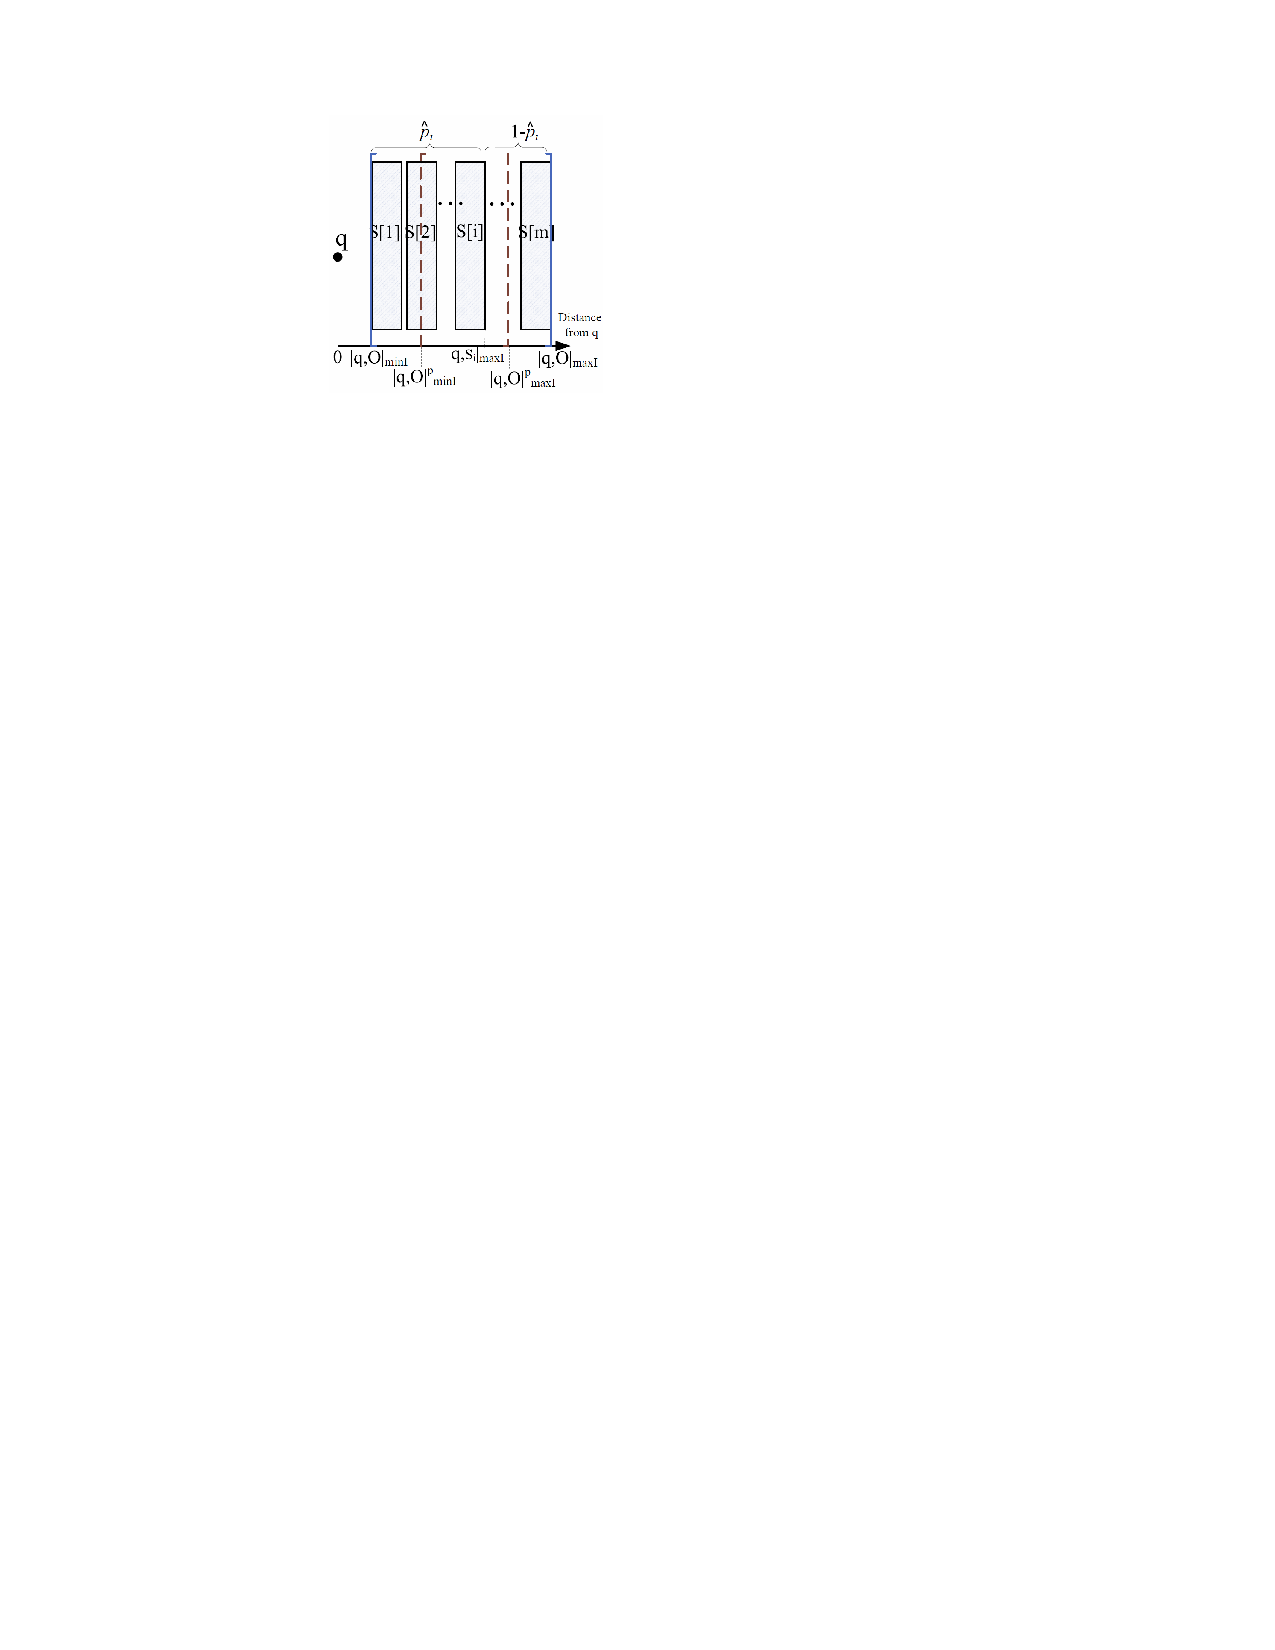
\includegraphics[width=\columnwidth]{figures/2-6/2-6-6.pdf}
  \end{figure}

  \column{0.7\textwidth}
  \begin{lemma}[Markov Lower Bounds]
    Suppose object $O$ overlaps with $m$ partitions $(O = \cup_{i=1}^{m}S[i])$, and $S[i]$s are sorted according to the minimum distance to a given point $q$. Use $\widehat{p_i}$ to denote $\sum_{j=1}^{i}p_i$. As $S[i]$ and $S[j]$ do not overlap, using \emph{Markov Inequality}, we have:
    \begin{equation*}
      E(|q, O|_I) \geq |q,S[i]|_{maxI} \cdot (1 - \widehat{p_i})
    \end{equation*}
  \end{lemma}

\end{columns}

\end{frame}

%------------------------------------------------

\begin{frame}
\frametitle{Bounds for Indoor Distances}

\conceptbf{Indoor Probabilistic ULBounds}

\vspace{10pt}
\begin{columns}[c]

  \column{0.3\textwidth}
  \begin{figure}[tb]
    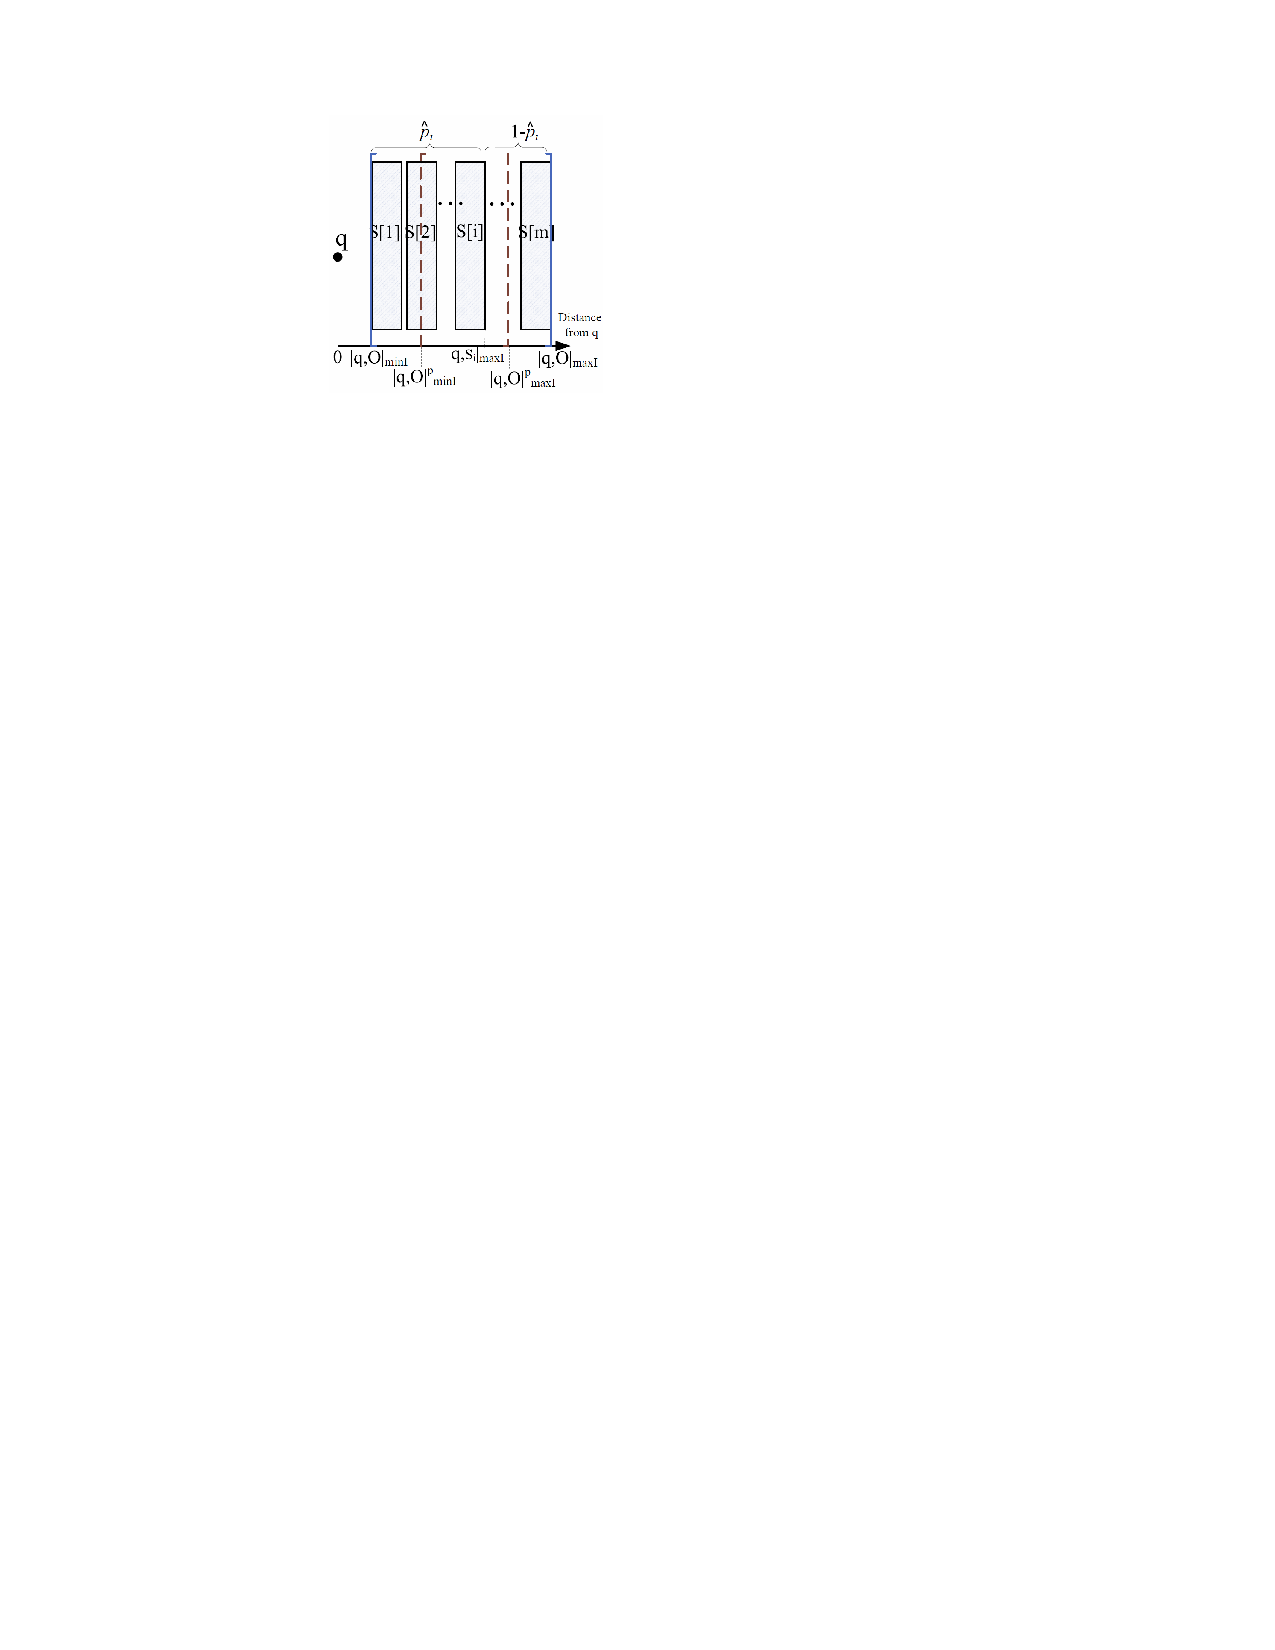
\includegraphics[width=\columnwidth]{figures/2-6/2-6-6.pdf}
  \end{figure}

  \column{0.7\textwidth}
  \begin{lemma}[Probabilistic ULBounds]
  \begin{equation*}
  \begin{split}
      & |q,S[i]|_{maxI} \cdot (1 - \widehat{p_i}) + |q, O|_{minI} \cdot \widehat{p_i} \\
      & \leq E(|q, O|_I) \leq \\
      & |q, O|_{maxI} \cdot (1 - \widehat{p_i}) + |q,S[i]|_{maxI} \cdot \widehat{p_i}
  \end{split}
  \end{equation*}
  \ssize{
  \textbf{Proof:} $ E(|q, O|_I)  = E(|q, \cup_{j \leq i}S[j]|_I) \cdot \widehat{p_i} +$\\
  $ E(|q, \cup_{k > i}S[k]|_I) \cdot (1 - \widehat{p_i})$. Since $|q,S[i]|_{maxI} \geq E(|q, \cup_{j \leq i}S[j]|_I) \geq |q,O|_{minI}$, and $|q,O|_{maxI} \geq E(|q, \cup_{k > i}S[k]|_I) \geq |q,O|_{minI}$, by substitution, the lemma is proved.
  }
  \end{lemma}

\end{columns}

\end{frame}

%------------------------------------------------

\begin{frame}
\frametitle{Summary}

use \emph{topological ULBounds} for the case that an object overlaps with a single partition; \\~\\

use \emph{probabilistic ULBounds} for the case that an object overlaps with multiple partitions.

\begin{figure}[tb]
  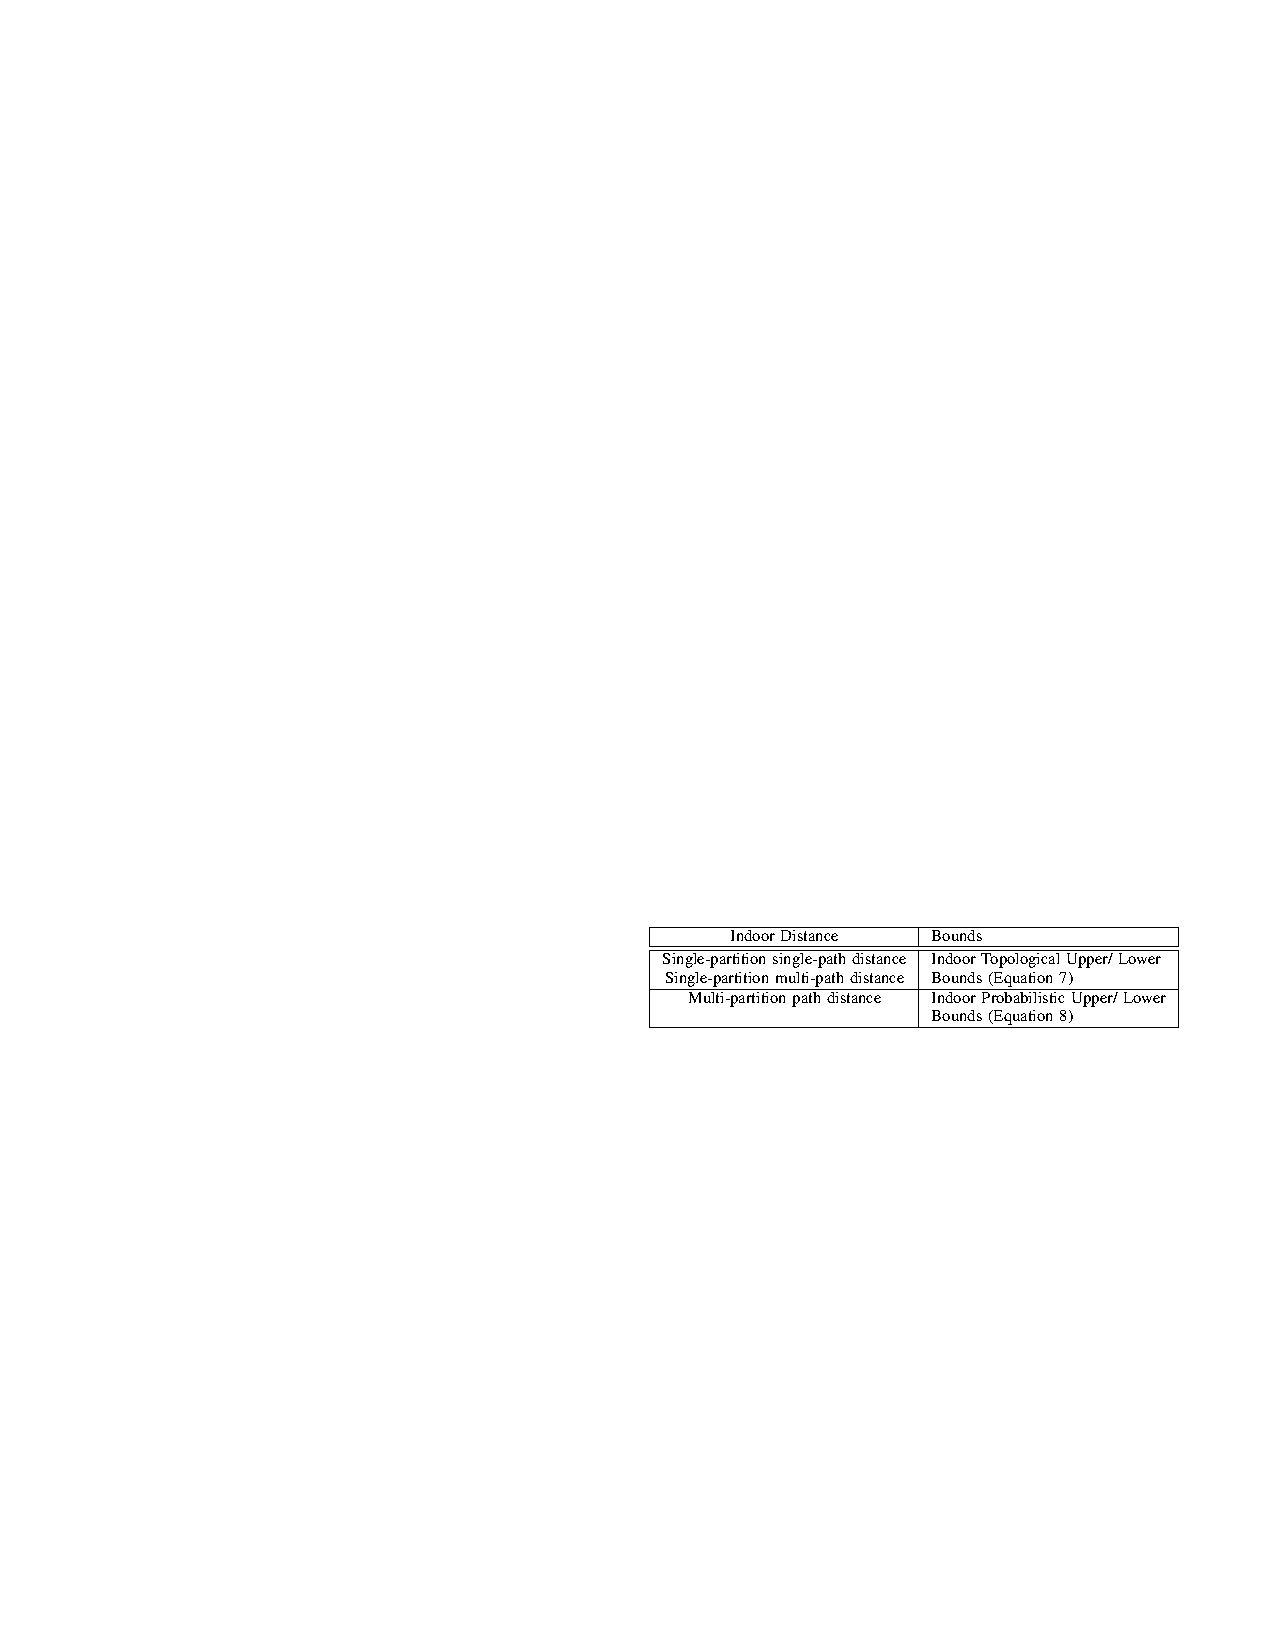
\includegraphics[width=0.7\columnwidth]{figures/2-6/2-6-7.pdf}
\end{figure}

with the Upper and Lower Bounds, as well as the approximate indoor distance, one can avoid computing shortest paths for all existential instances of an uncertain objects.

\end{frame}

%------------------------------------------------

\begin{frame}
\frametitle{Composite Index for Indoor Space}

\begin{columns}[c]

  \column{0.5\textwidth}
  \begin{figure}[tb]
    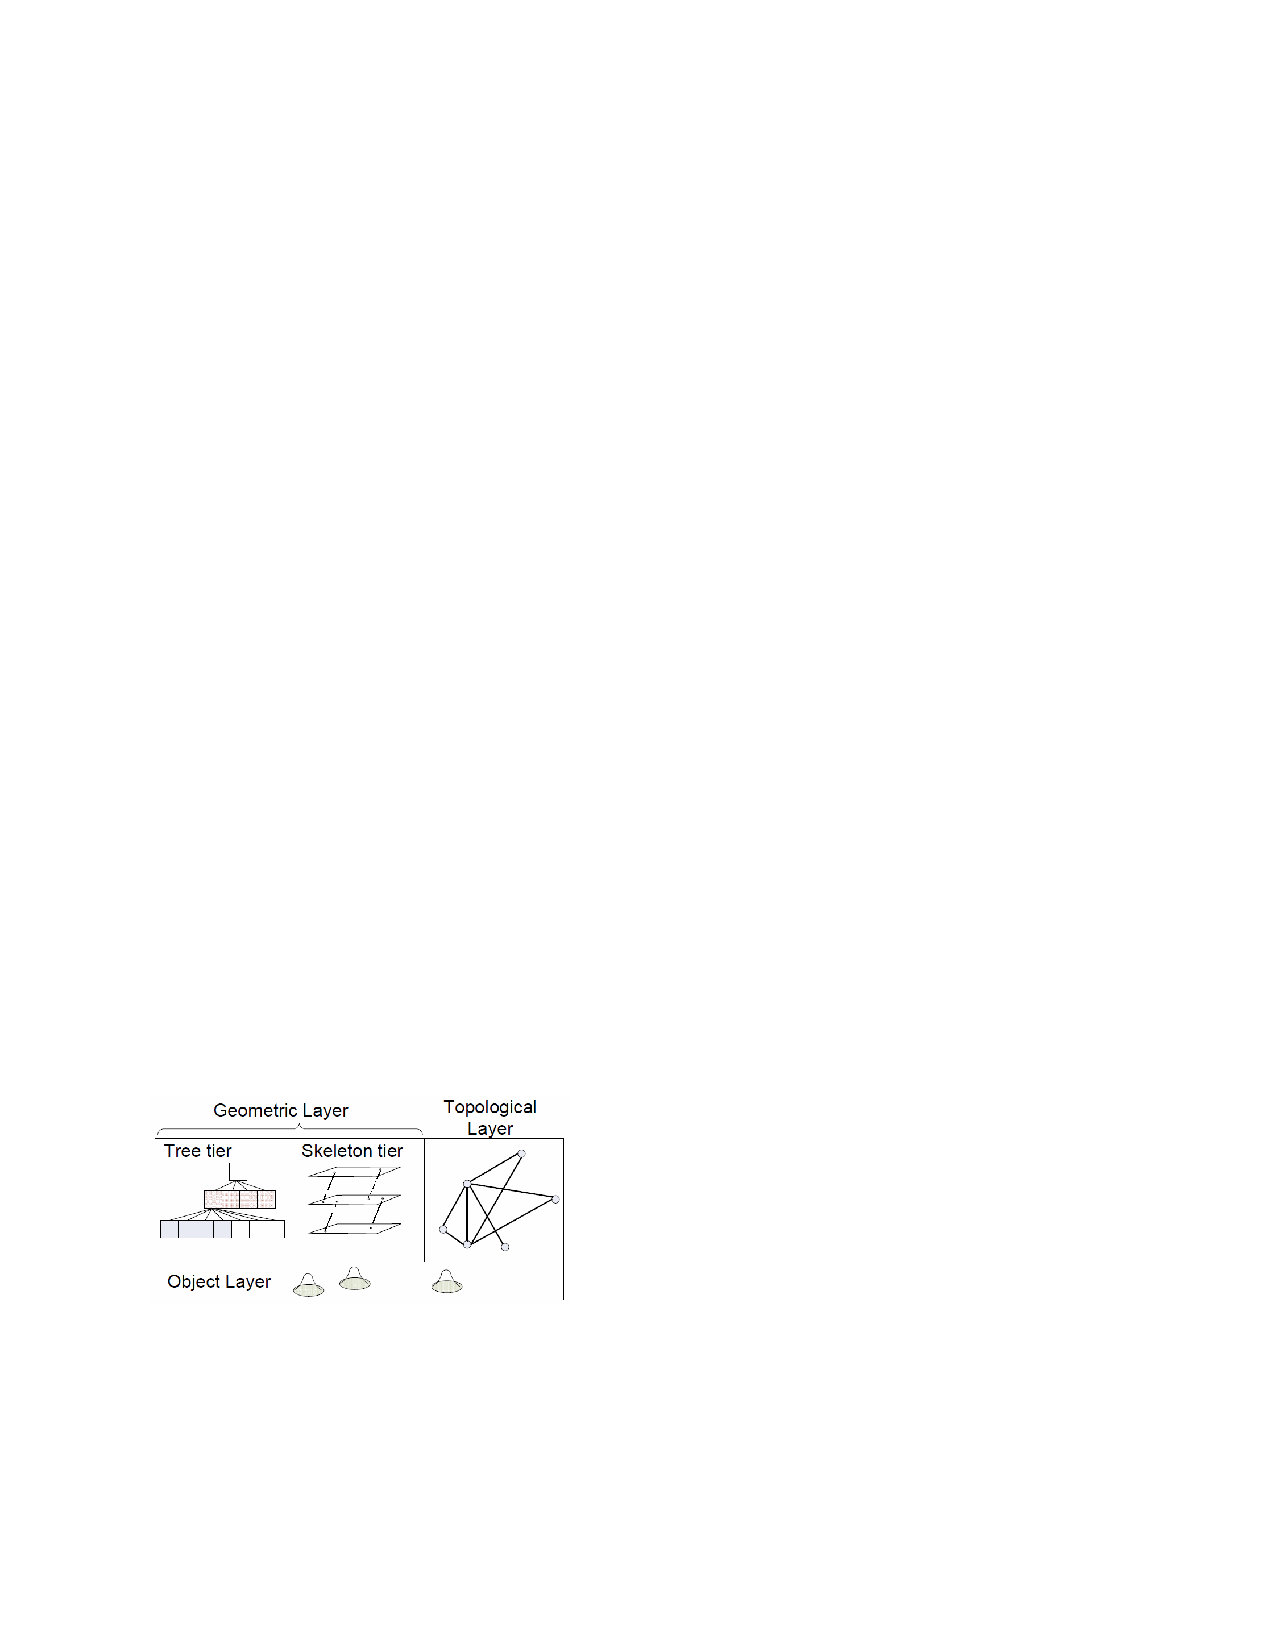
\includegraphics[width=\columnwidth]{figures/2-6/2-6-8.pdf}
  \end{figure}

  \column{0.5\textwidth}
  \begin{fitemize}
    \item \conceptbf{geometric layer} consists of a tree structure that adapts the R$^*$-tree to index all partitions, as well as a skeleton tier that maintains a small number of distances between staircases.
    \item \conceptbf{topological layer} maintains the connectivity information between indoor partitions.
    \item \conceptbf{object layer} stores all indoor moving objects and is associated with the tree through partitions at its leaf level.
  \end{fitemize}

\end{columns}

\end{frame}

%------------------------------------------------

\begin{frame}
\frametitle{Composite Index: Overview}

\begin{figure}[tb]
  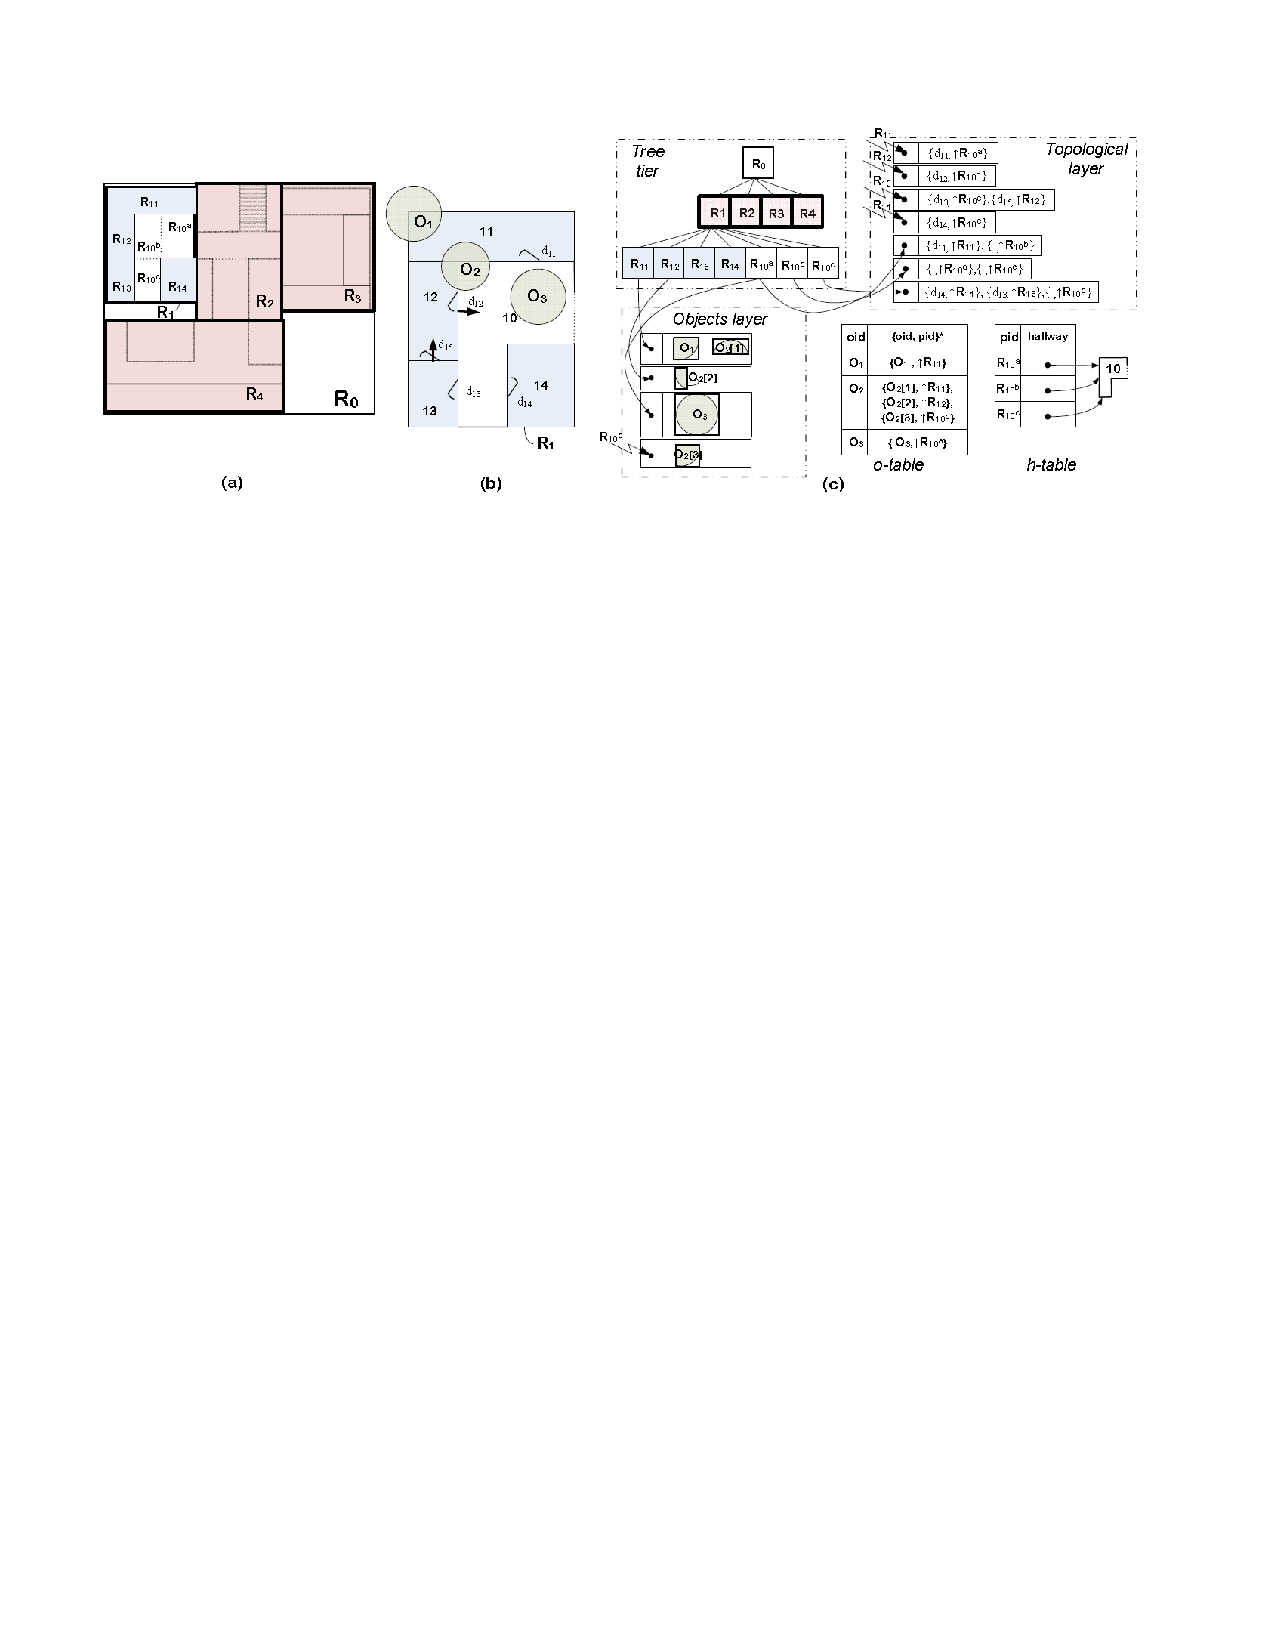
\includegraphics[width=\columnwidth]{figures/2-6/2-6-9.pdf}
\end{figure}

\end{frame}

%------------------------------------------------

\begin{frame}
\frametitle{Composite Index: Tree Tier}

\begin{fitemize}
  \item instead of 3D $Minimum Bounding Rectangle$, when creating the tree, set the vertical length for one partition to 1 centimeter. Two advantage: 1) reduce the distance calculation workload; 2) makes the distance reflected in the tree more accurate without the disturbance from the vertical dimension.
  \item the imbalanced partition are decomposed to small but regular region, each is called an \emph{index unit}.
  \item A hash table is used to map such an index unit to its original indoor partition.
\end{fitemize}

\vspace{-10pt}
\begin{figure}[tb]
  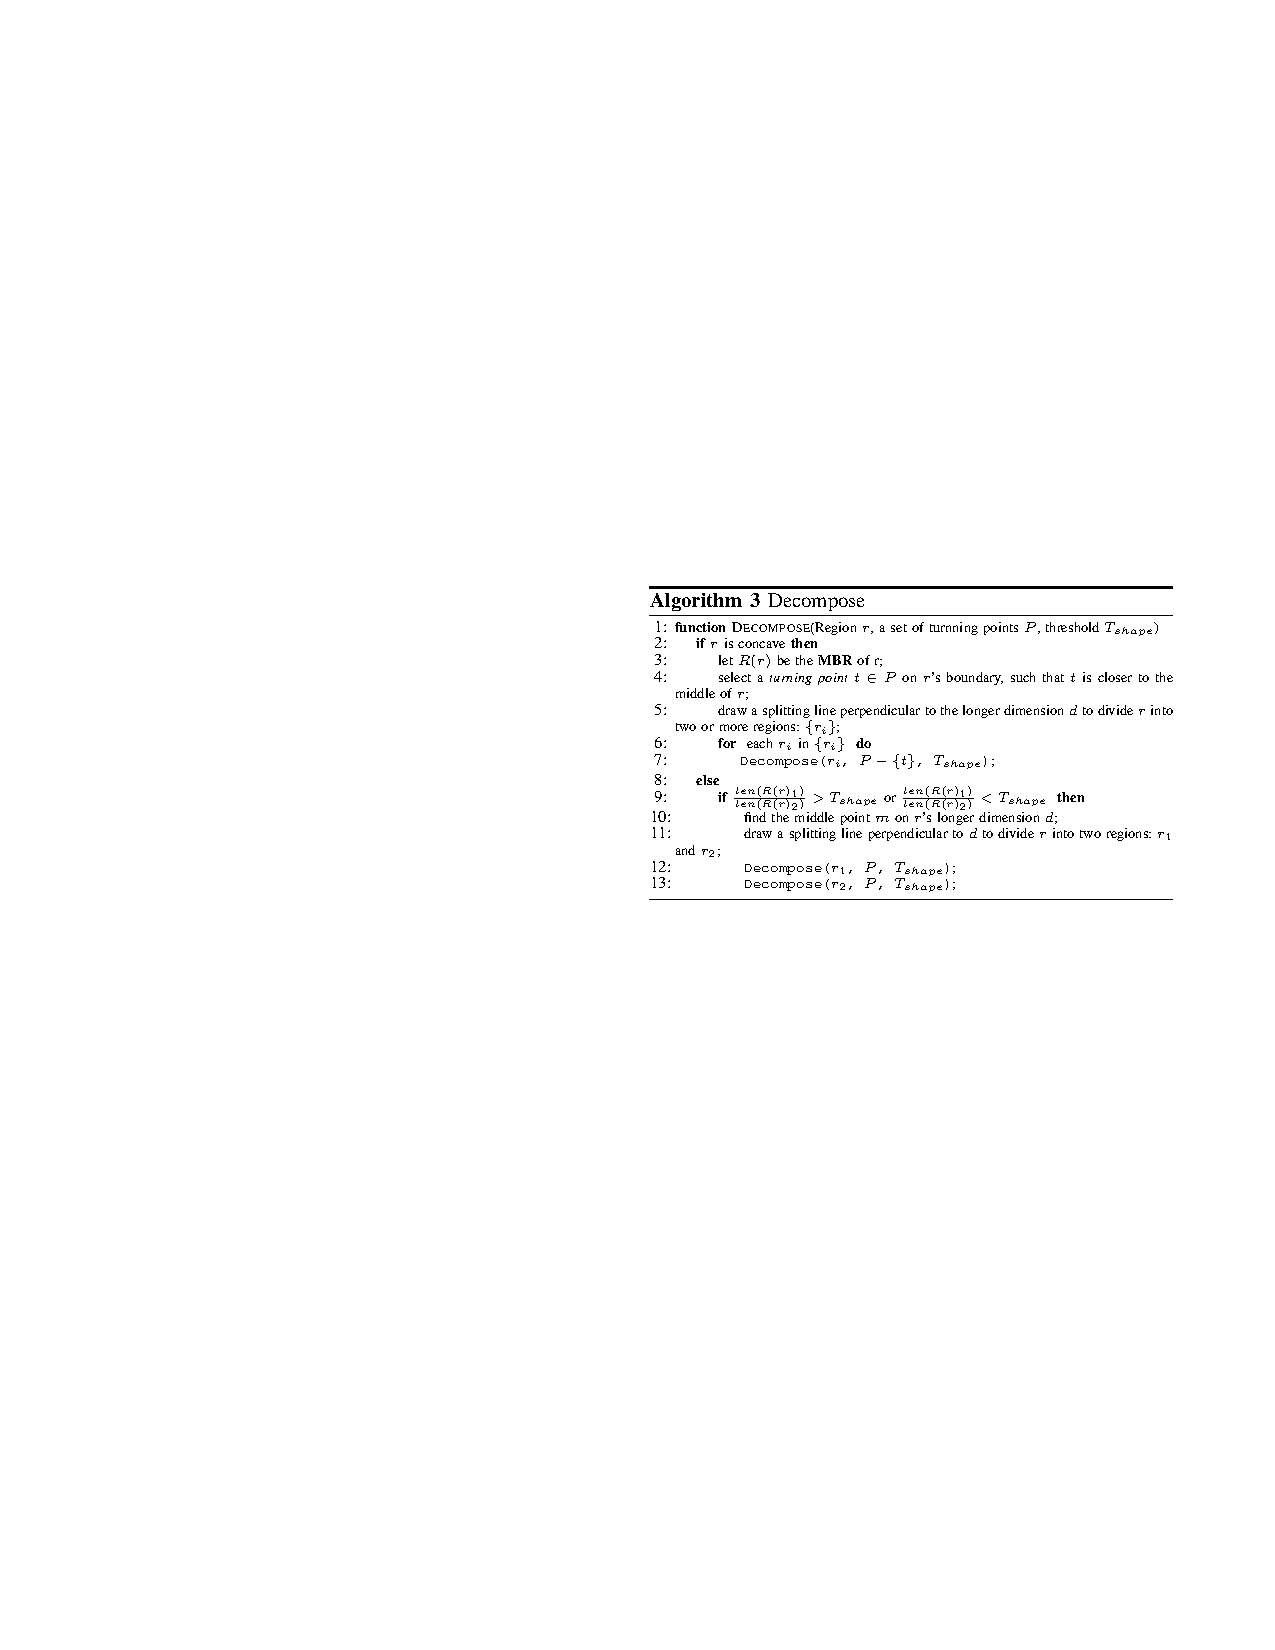
\includegraphics[width=0.55\columnwidth]{figures/2-6/2-6-10.pdf}
\end{figure}

\end{frame}

%------------------------------------------------

\begin{frame}
\frametitle{Composite Index: Object Tier}

A hash table $o-table$

\begin{equation*}
  o-table : \{ O \} \rightarrow 2^{\{index~unit\}}
\end{equation*}

$o-table$ maps an object to all the index units it overlaps, and it is tightly tie up with the tree tier.\\~\\

When an object update occurs, $o-table$ needs to be updated accordingly.

\end{frame}

%------------------------------------------------

\begin{frame}
\frametitle{Composite Index: Topological Tier}

This layer maintains the connectivity between partitions. Each leaf node stores a (sub)partition.\\~\\

For accessibility, the doors belonging to the partitions are also stored, as well as the the links to accessible partitions through each door.

\end{frame}

%------------------------------------------------

\begin{frame}
\frametitle{Composite Index: Skeleton Tier}

Skeleton Tier is a graph, each staircase entrance is captured as a graph node, and an edge connects two nodes if their entrances are on the same floor or their entrances belong to the same staircase.\\~\\

The weight of an edge is the indoor distance between the two staircase entrances.

\vspace{-10pt}
\begin{columns}[c]

  \column{0.4\textwidth}
  \begin{figure}[tb]
    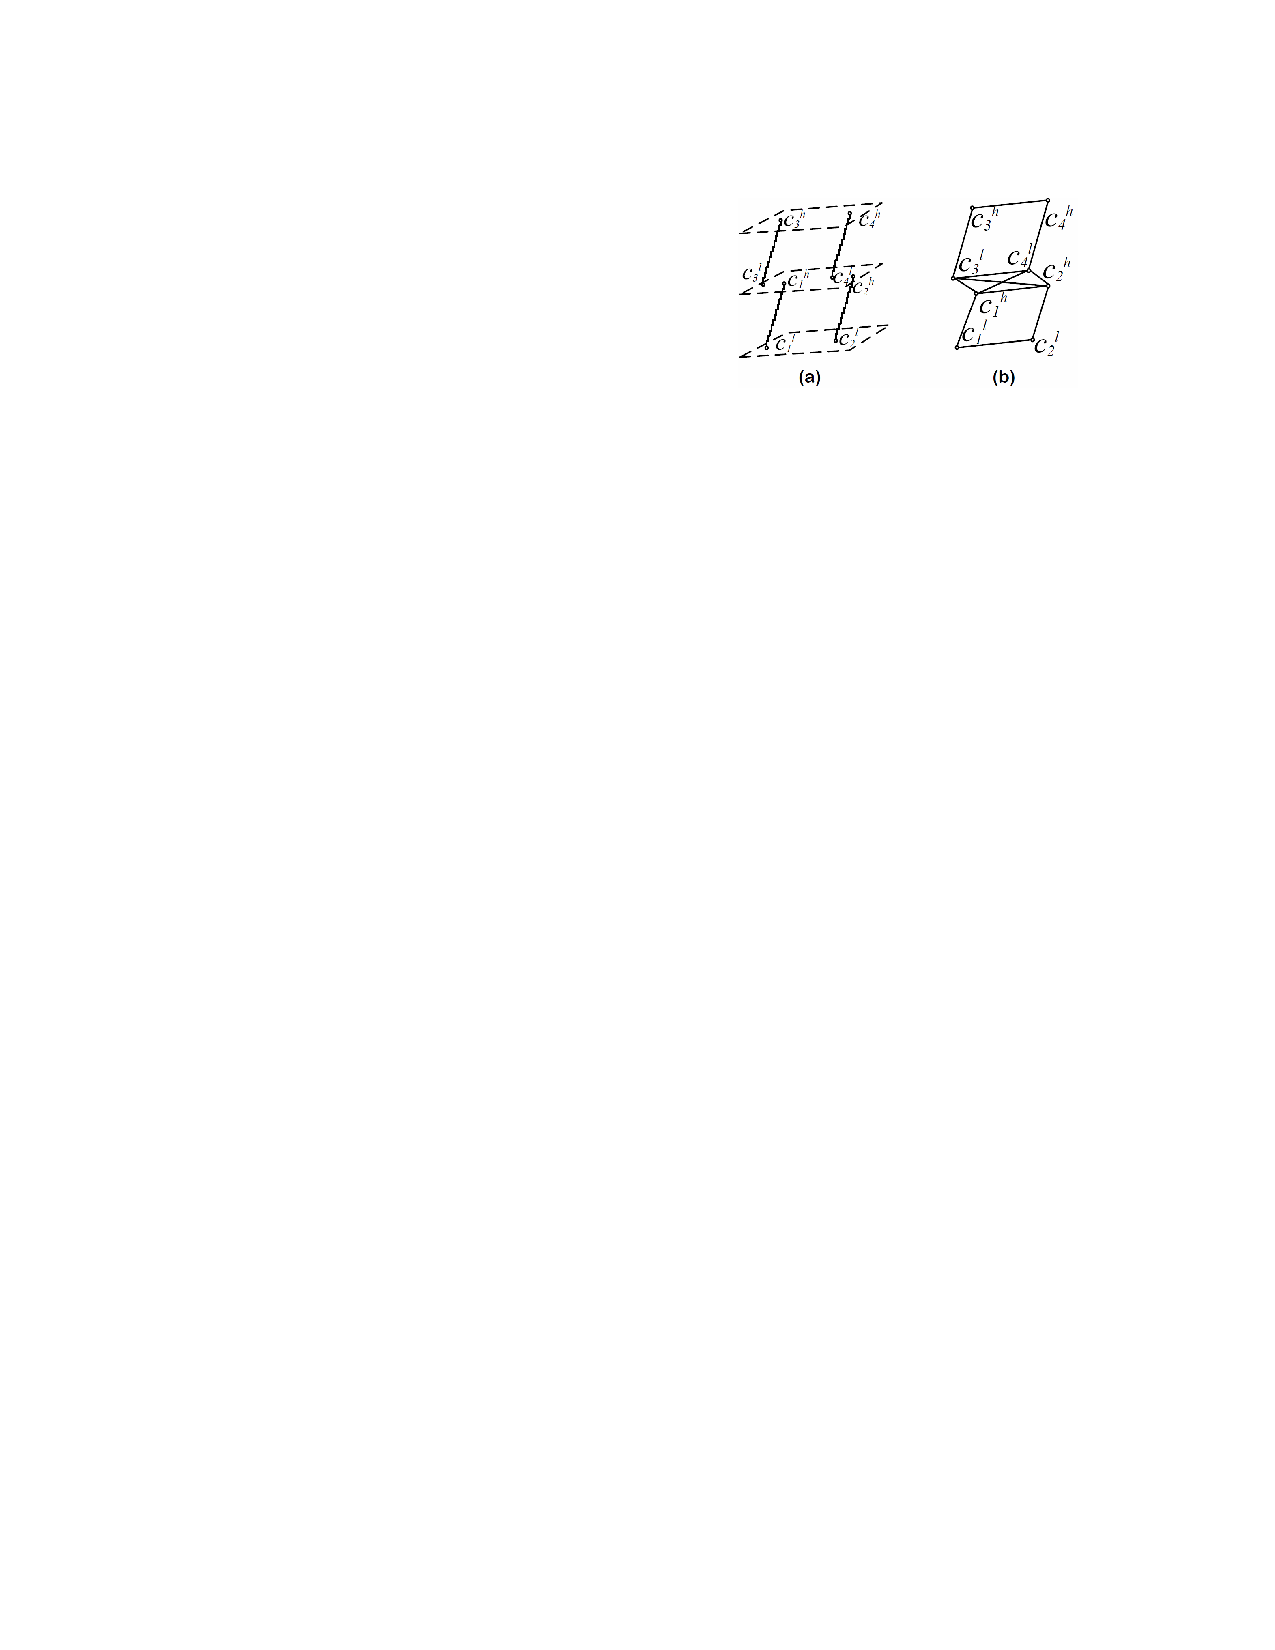
\includegraphics[width=\columnwidth]{figures/2-6/2-6-11.pdf}
  \end{figure}

  \column{0.6\textwidth}
  \ssize{
  \begin{definition}[staircase distance matrix $M_{s2s}$]
    \begin{sitemize}
      \item $M_{s2s}[s_i,s_i] = 0$;
      \item $M_{s2s}[s_i,s_j] = |s_i, s_j|_E$ if $s_i$ and $s_j$ are on the same floor;
      \item if $s_i$ and $s_j$ are of a same staircase, $M_{s2s}[s_i,s_j]$ is the shortest distance from $s_i$ to $s_j$ within that staircase;
      \item $M_{s2s}[s_i,s_j]$ is calculated as the shortest path distance from $s_i$ to $s_j$ in the skeleton layer for other cases.
    \end{sitemize}
  \end{definition}
  }

\end{columns}

\end{frame}

%------------------------------------------------

\begin{frame}
\frametitle{Skeleton Distance}

\textrm{Let $q$ be a fixed indoor point, $q.f$ the floor of $q$, and $S(q.f)$ all the staircases on floor $q.f$.}

\vspace{10pt}
\begin{definition}[Skeleton Distance]
  Given two points $p$ and $q$, their skeleton distance $|q,p|_K = |q,p|_E$ if they are on the same floor; otherwise, $|q,p|_K = \min_{s_q \in S(q.f), s_p \in S(p.f)}(|q,s_q|_E + M_{s2s}[s_q,s_p] + |s_p, p|_E)$.
\end{definition}

\vspace{10pt}
Define the skeleton distance as the alternative \emph{Geometric Distance}.

\end{frame}

%------------------------------------------------

\begin{frame}
\frametitle{Indoor Distance Bounds in the Geometric Layer}

\begin{lemma}[Geometric Lower Bound Property]
  Given two points $p$ and $q$, their skeleton distance lower bounds their indoor distance, i.e., $|q,p|_K \leq |q,p|_I$.\\~\\
  \textbf{Proof:}~If $q$ and $p$ are on the same floor, $|q,p|_K = |q,p|_E \leq |q,p|_I$. Otherwise, suppose $s_{q}^{*} \in S(q.f)$ and $s_{p}^{*} \in S(p.f)$ are on the shortest path from $q$ to $p$, denoted by $q \overset{*s_{q}^{*}*s_{p}^{*}}{\rightarrow} p$. Since $|q,p|_K = \min_{s_q \in S(q.f), s_p \in S(p.f)}(|q,s_q|_E + M_{s2s}[s_q,s_p] + |s_p, p|_E) \leq |q,s_{q}^{*}|_E + M_{s2s}[s_{q}^{*},s_{p}^{*}] + |s_{p}^{*}, p|_E = |q,p|_I$, the lemma is proved.
\end{lemma}

\end{frame}

%------------------------------------------------

\begin{frame}
\frametitle{Indoor Distance Bounds in the Geometric Layer}

Consider an entity $e$ that is either an object or an $ind$R-tree node. If $e$ spans multiple floors, we use interval $[e.lf,e.uf]$ to represent all those floors. Note those floors must be consecutive. We define the minimum skeleton distance $|q,e|_{minK}$:

\begin{figure}[tb]
  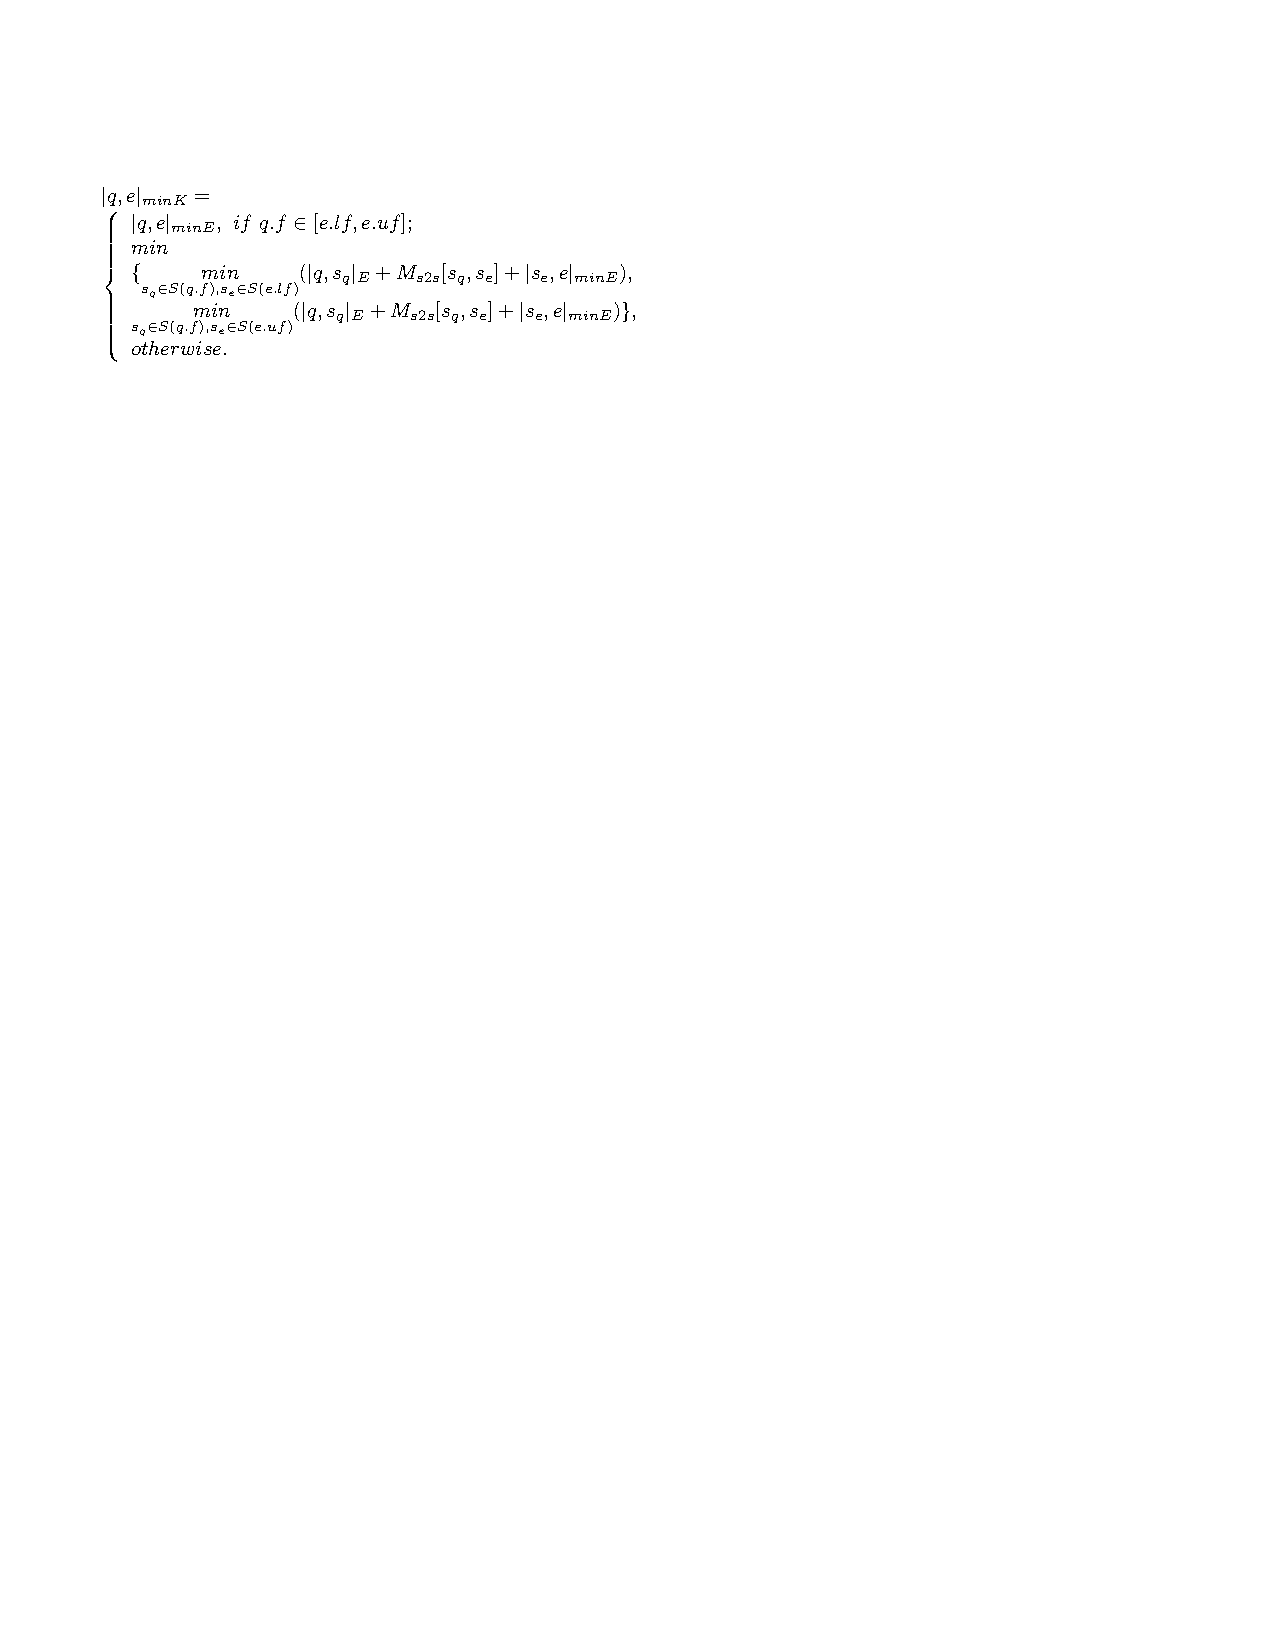
\includegraphics[width=0.7\columnwidth]{figures/2-6/2-6-12.pdf}
\end{figure}

With $|q,e|_{minK}$, one can constrain the search via the $ind$R-tree to a much smaller range compared to if use the Euclidean distance bounds.

\end{frame}

%------------------------------------------------

\begin{frame}
\frametitle{Dynamic Operations on the Topological Layer}

\textbf{Insertion.}~\textrm{When the topological change leads to a new indoor partition $P$, $P$(or its sub-partitions due to decomposition) is inserted into the $ind$R-tree, its leaf node is connected to the adjacent partitions, and the $h-table$ is updated if a decomposition is invovled.}\\~\\

\textbf{Deletion.}~\textrm{From the $ind$R-tree to remove a partition $P$ to be deleted, the links involving $P$ are removed from the adjacent partitions, and $P$'s entry in the $h-table$ is deleted if $P$ is a decomposed sub-partition.}

\end{frame}

%------------------------------------------------

\begin{frame}
\frametitle{Dynamic Operations on the Object Layer}

\textbf{Insertion.}~\textrm{To insert an object $O$, search the $ind$R-tree to find the leaf nodes $\{ P_i \}$ that overlap with $O$'s uncertainty region. Also insert a new entry to $o-table$.}\\~\\

\textbf{Deletion.}~\textrm{To delete an object $O$, use the $o-table$ to find the $ind$R-tree leaf nodes $\{ P_i \}$ that overlap with $O$'s uncertainty region. For each $P_i$, $O$ is removed from its associated bucket. Also the entry for $O$ is deleted from the $o-table$.}

\end{frame}

%------------------------------------------------

\begin{frame}
\frametitle{Query Semantics}

\begin{definition}[Indoor Range Query, iRQ]
  Given a query point $q \in \mathbb{I}$ and a distance value $r$, the \emph{iRQ} returns objects whose indoor distances are smaller than $r$. Formally, $iRQ_{q,r}(\mathbb{O}) = \{ O | |q,O|_I \leq r, O \in \mathbb{O}\}$.
\end{definition}

\begin{definition}[Indoor $k$ Nearest Neighbor Query, ikNNQ]
  Given a query point $q \in \mathbb{I}$ and a parameter $k$, the \emph{ikNNQ} returns $k$ objects whose indoor distances to $q$ are the smallest among all objects. Formally, $ikNN_{q,k}(\mathbb{O}) = \{ O | O \in \mathbb{O}\}$, where $|ikNN_{q,k}(\mathbb{O})| = k, \forall O_i \in ikNN_{q,k}(\mathbb{O}), \forall O_j \in \mathbb{O} \setminus ikNN_{q,k}(\mathbb{O}), |q,O_i|_I \leq |q,O_j|_I$.
\end{definition}

\end{frame}

%------------------------------------------------

\begin{frame}
\frametitle{Efficient Query Evaluation}

\begin{enumerate}
  \fsize{
  \item \conceptbf{Filtering Phase} locates the source partition that contains the query point and retrieves condidate partitions as well as candidate objects.
  \item \conceptbf{Subgraph Phase} constructs a subgraph based on candidate partitions, and uses the doors of the source partition as sources to compute the shortest indoor paths that are to be used in the subsequent two phases.
  \item \conceptbf{Prunning Phase}, upper/lower distance bounds for objects are calculated to further reduce the number of candidate objects.
  \item \conceptbf{Refinement Phase}, the indoor distances for the remaining objects are computed and the qualifying objects are returned as the query results.
  }
\end{enumerate}

\end{frame}

%------------------------------------------------

\begin{frame}
\frametitle{Indoor Range Query}

\begin{columns}[c]

  \column{0.2\textwidth}
  \begin{figure}[tb]
    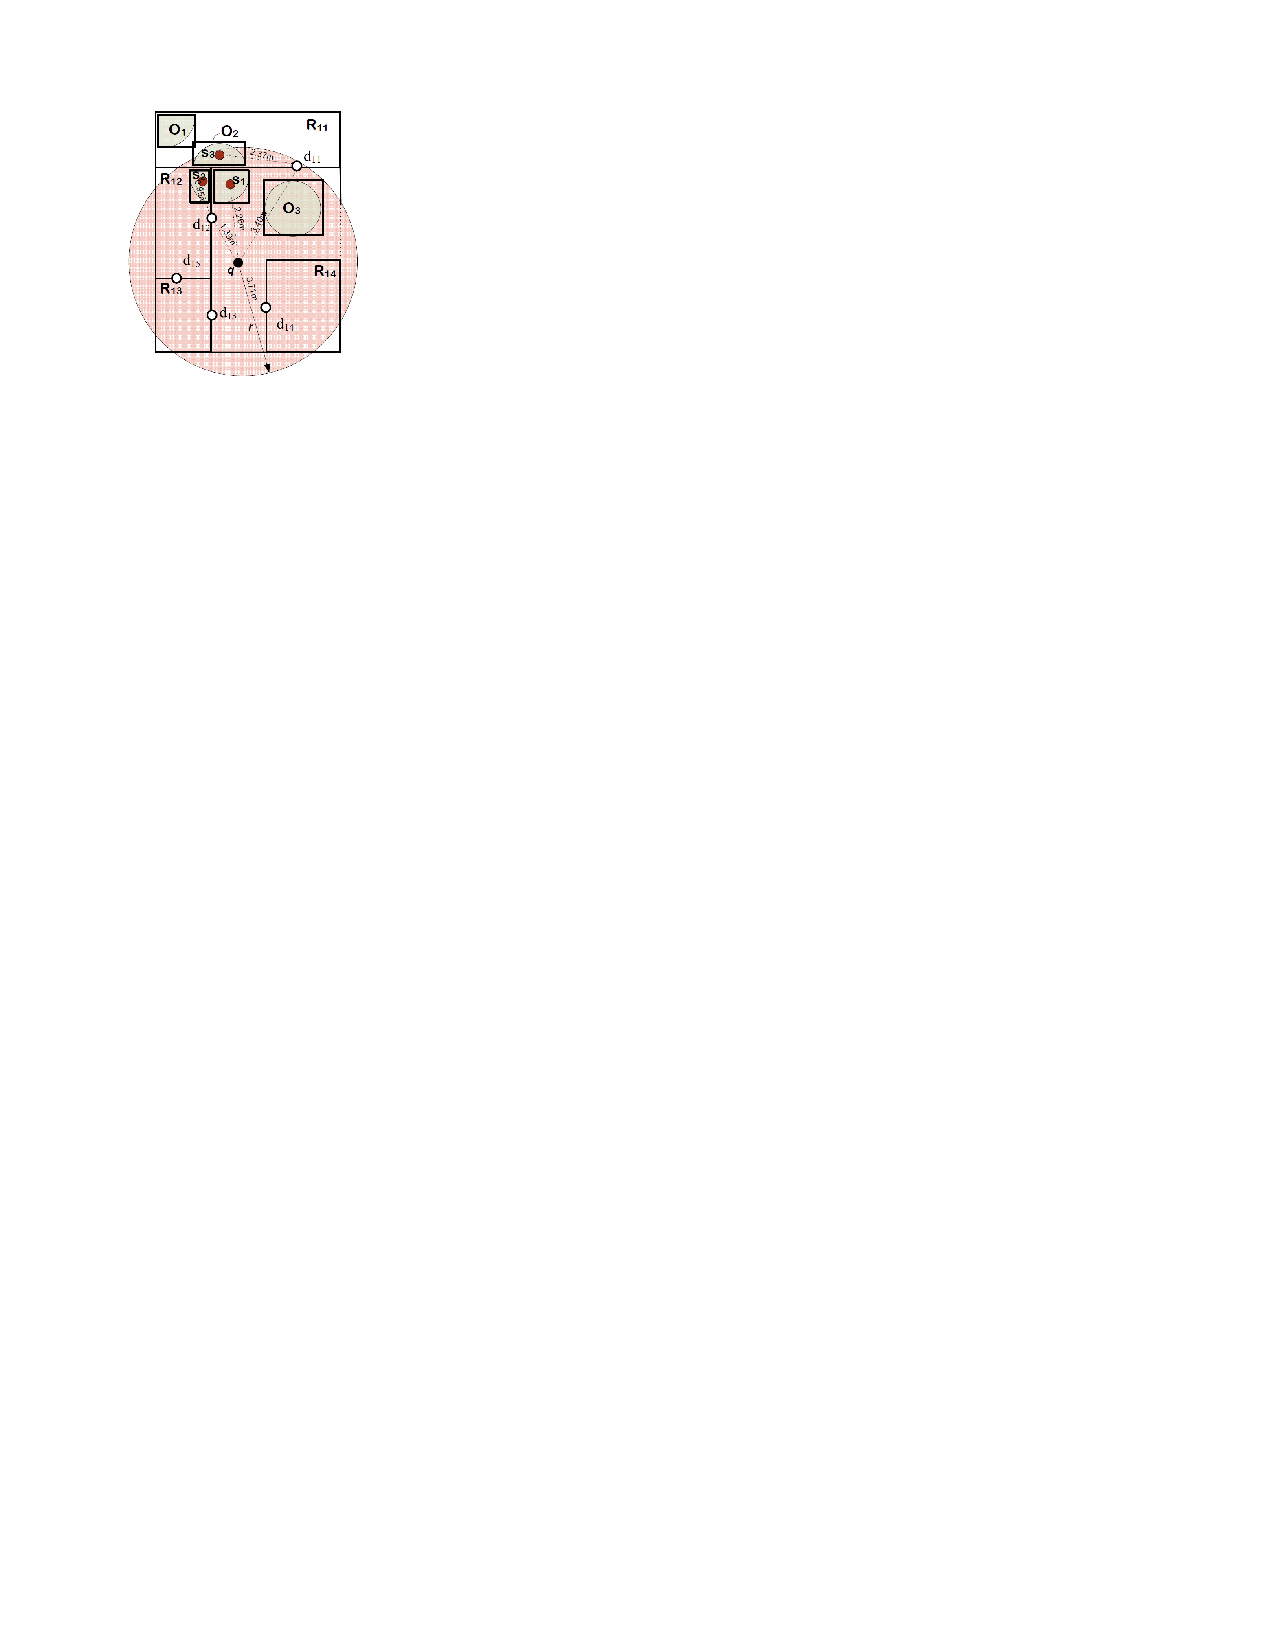
\includegraphics[width=\columnwidth]{figures/2-6/2-6-13.pdf}
  \end{figure}


  \column{0.8\textwidth}
  \begin{example}
    \ssize{
    The circle $\bigodot(q,r)$ is the query region represented in the Euclidean space. Object $O_1$ is pruned away in filtering phase, since $|q, O_1|_{minE} > r$. After deriving the upper/lower bounds for the remaining objects in the pruning phase, $O_3$ is qualified. For the undetermined object $O_2$, the exact indoor distance is calculated and compared to $r$.
    }
  \end{example}

\end{columns}

\begin{columns}[c]

  \column{0.4\textwidth}
  \begin{figure}[tb]
    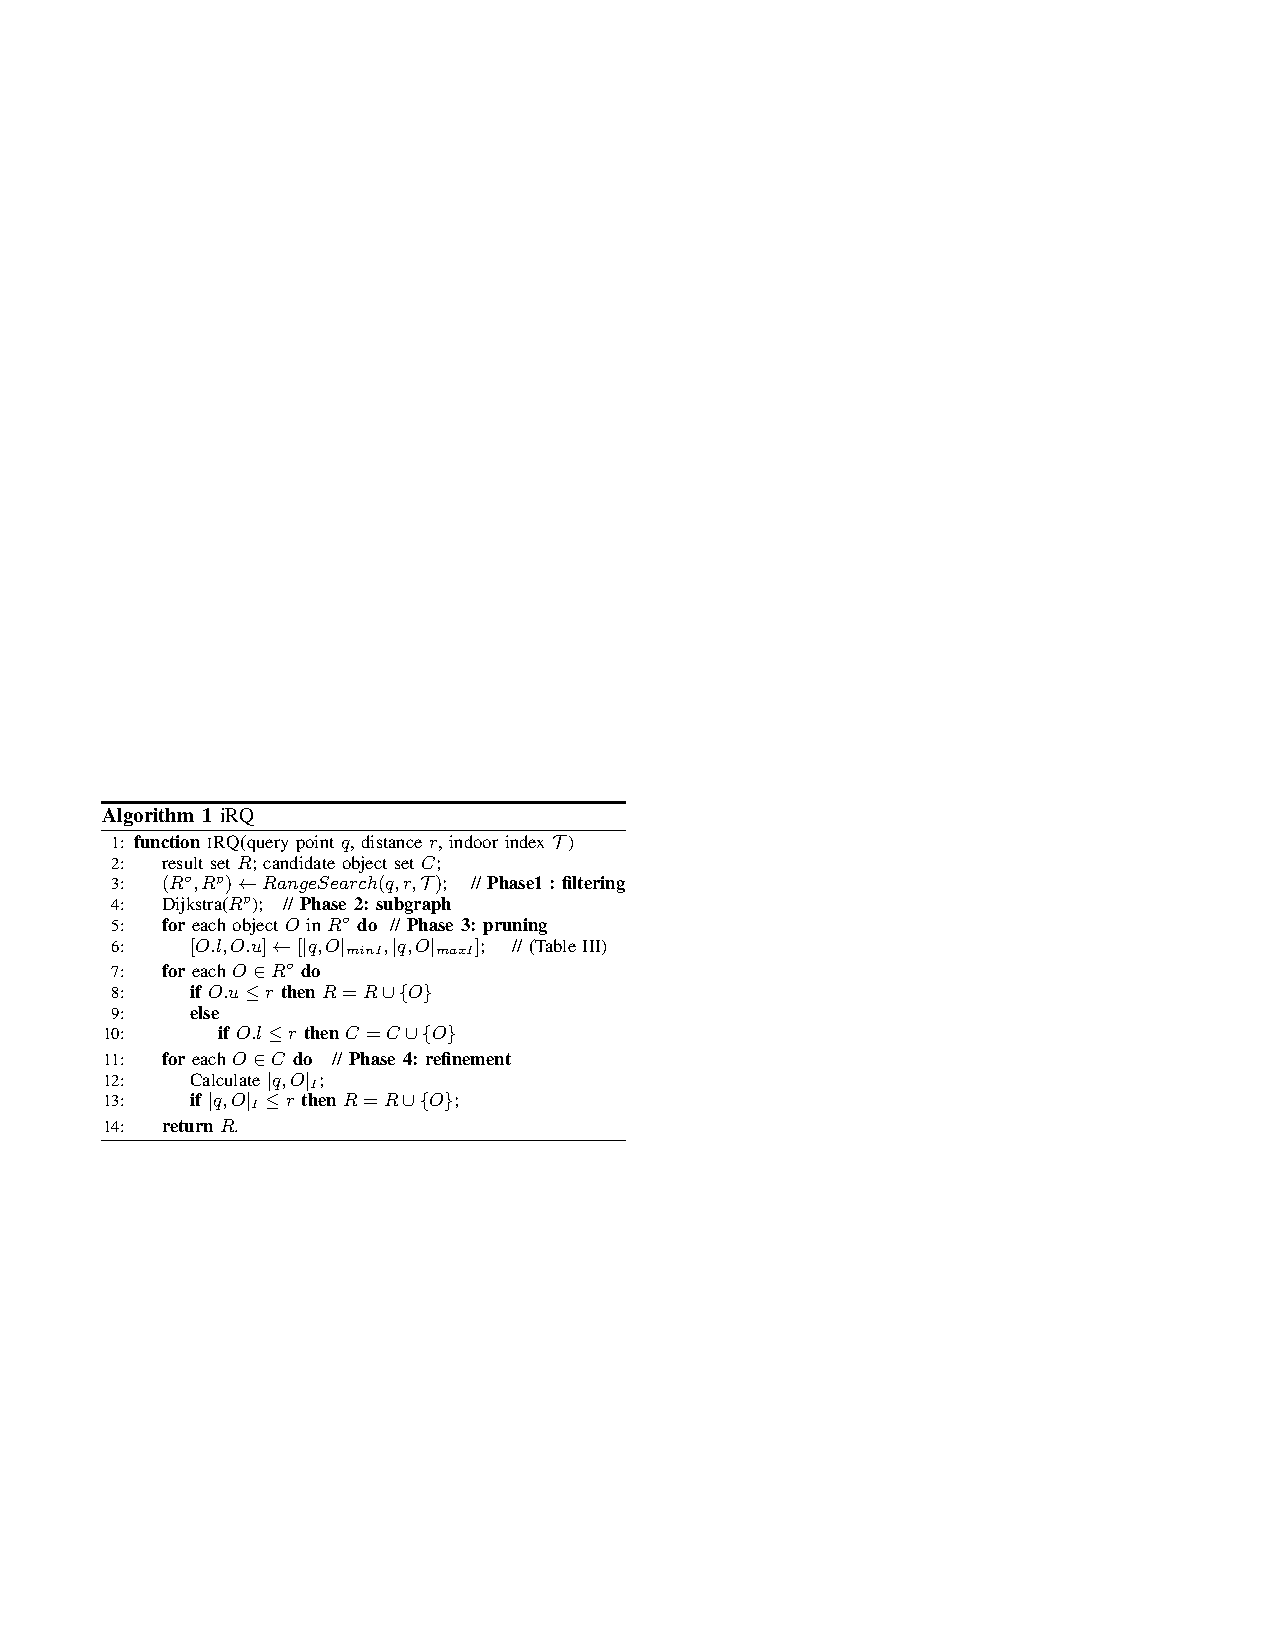
\includegraphics[width=\columnwidth]{figures/2-6/2-6-14.pdf}
  \end{figure}

  \column{0.6\textwidth}
  \begin{sitemize}
    \item in the filtering, iRQ calls $RangeSearch$ to search the geometric layer.
    \item lines 5--10: iRQ makes use of the topological upper/lower bounds to approximate indoor distances and compare them to $r$.
    \item lines 11--13: the exact indoor distances are only computed for those objects whose bounds cover $r$.
  \end{sitemize}

\end{columns}

\end{frame}

%------------------------------------------------

\begin{frame}
\frametitle{Indoor $k$ Nearest Neighbor Query}

\begin{columns}[c]

  \column{0.16\textwidth}
  \begin{figure}[tb]
    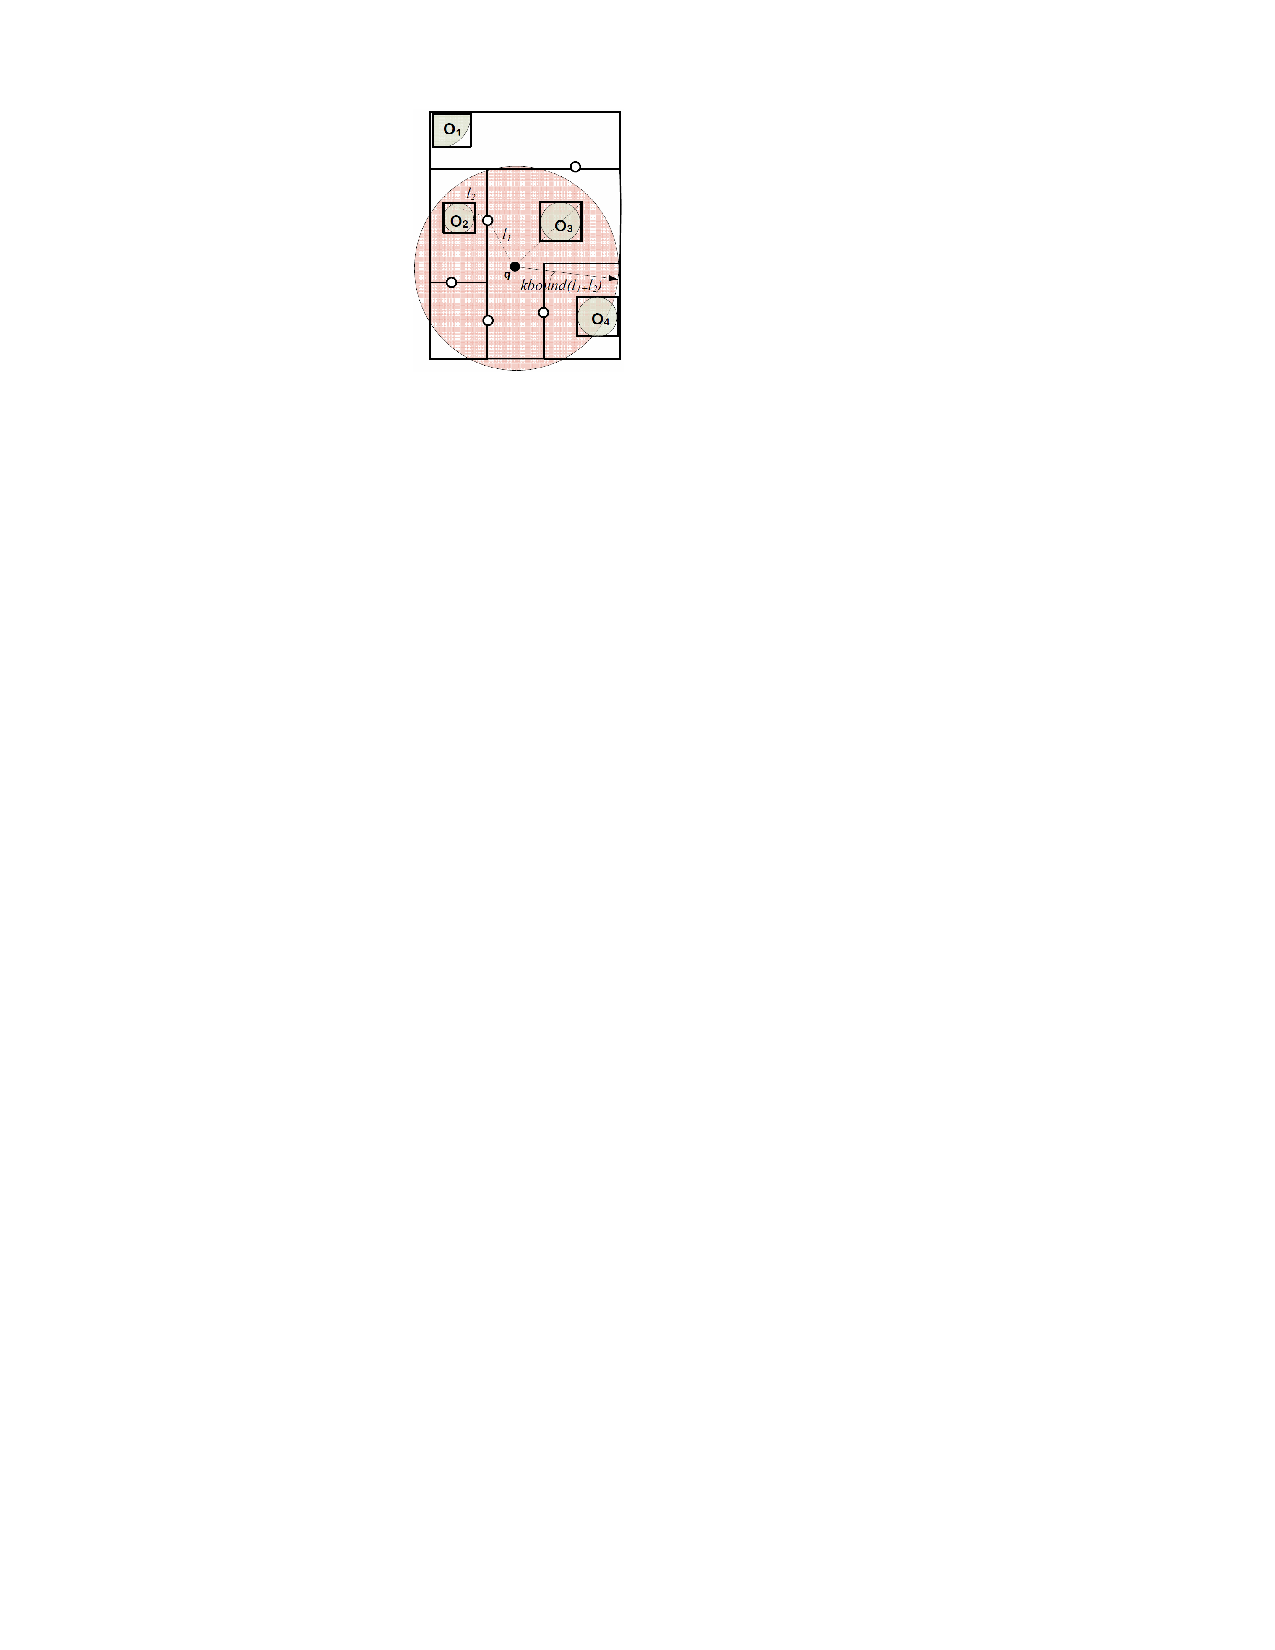
\includegraphics[width=\columnwidth]{figures/2-6/2-6-15.pdf}
  \end{figure}


  \column{0.84\textwidth}
  \begin{example}
    \ssize{
    $kSeedsSelection$ finds $O_2$ and $O_3$ as seeds. Because $O_2$'s topological looser upper bound is longer, it is chosen as the kbound. Through the range search, $O_1$ is excluded since $|q,O_1|_K > kbound$.
    }
  \end{example}

\end{columns}

\begin{columns}[c]

  \column{0.35\textwidth}
  \begin{figure}[tb]
    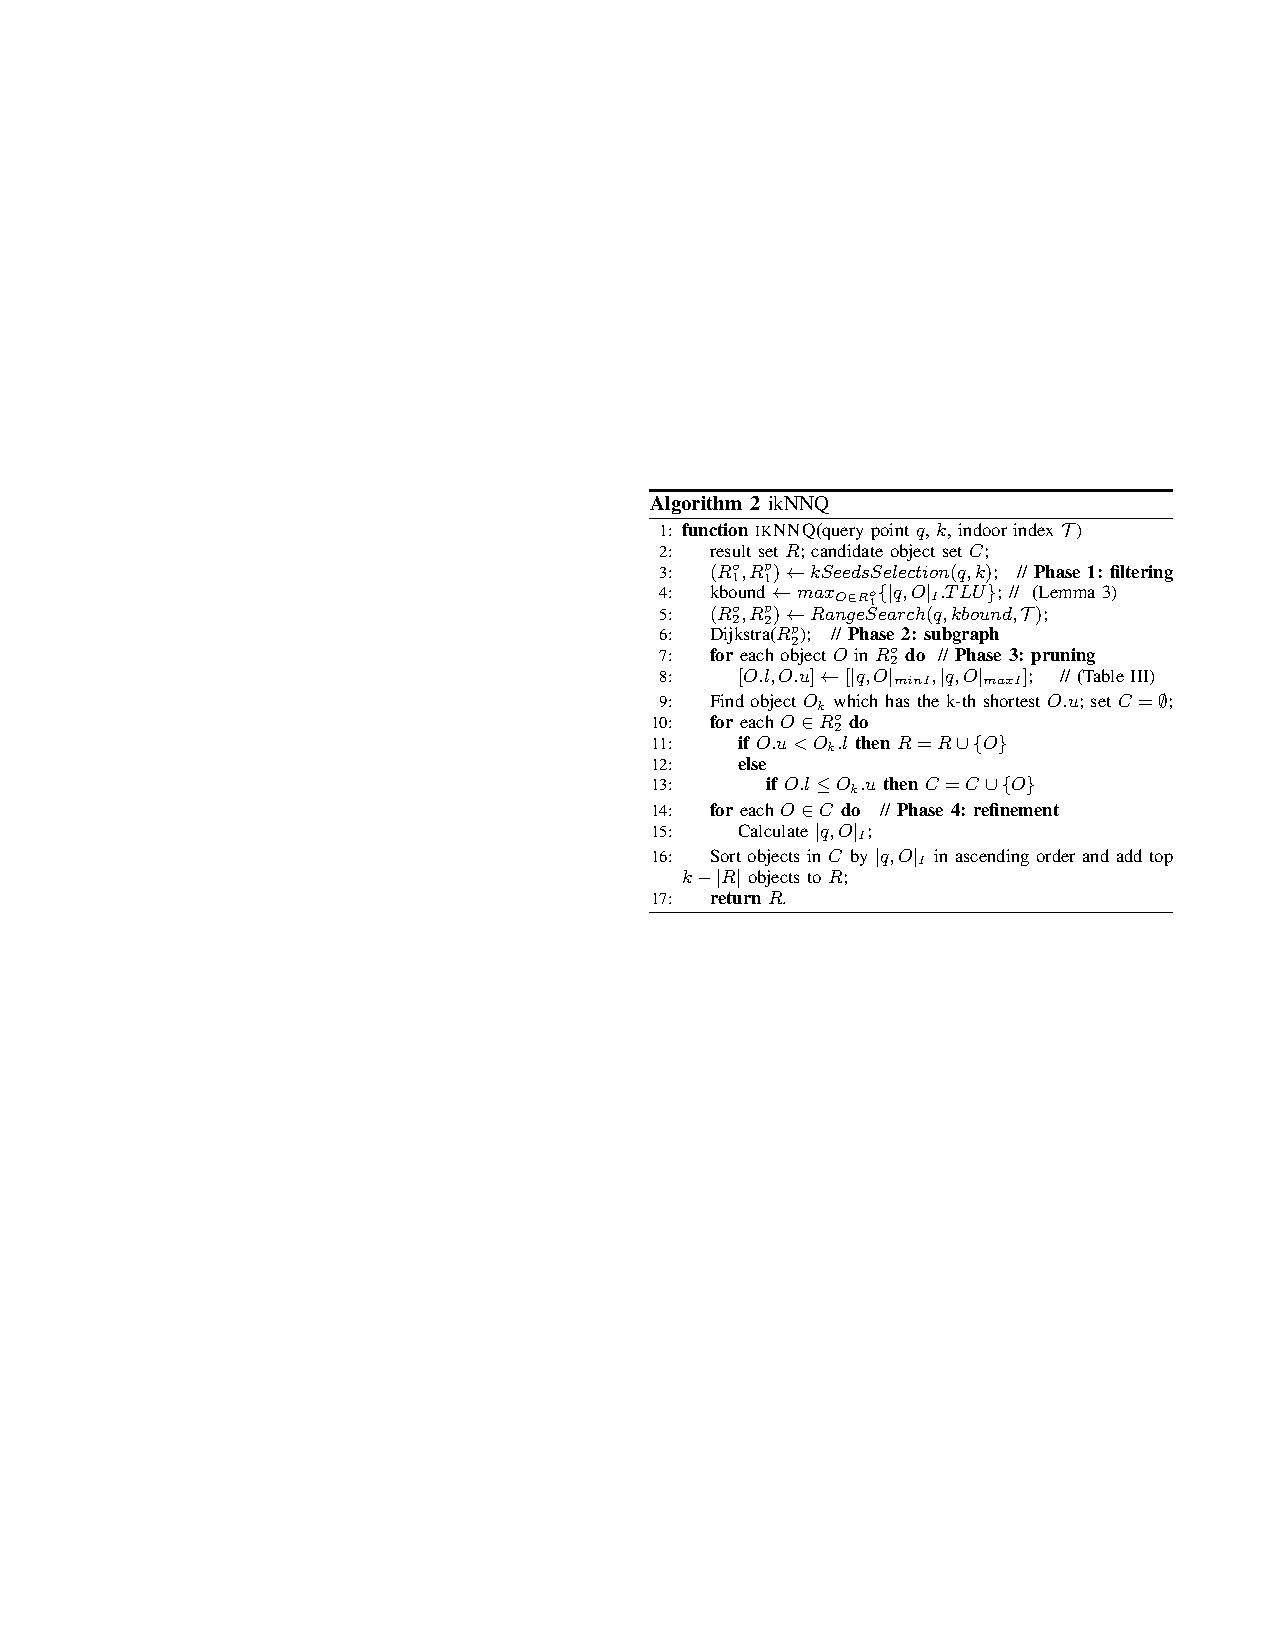
\includegraphics[width=\columnwidth]{figures/2-6/2-6-16.pdf}
  \end{figure}

  \column{0.65\textwidth}
  \begin{sitemize}
    \item in the filtering, ikNNQ calls $kSeedsSelection$ to return an object $R_1^o$ and a partition set $R_1^p$.
    \item $R_1^o$ contains $k$ objects taht are in query point $q$'s partition or in the closet adjacent partitions. $R_1^p$ is the set of all those involved partition.
    \item ikNNQ derives \emph{Topological Looser Upper Bounds} for the $k$ objects and choose the longest one as $kounds = \max_{seed_i \in R_1^o}\{ |q,seed_i|_I.TLU \}$.
    \item Line 4: a range search $\bigodot(q,kound)$ is done on the tree tier.
  \end{sitemize}

\end{columns}

\end{frame}

%------------------------------------------------

\begin{frame}
  \frametitle{Research Directions}

  \begin{itemize}
  	\item it is of interest to study other query types using the distance bounds and the composite index proposed in this paper.
    \item it is useful to estimate the selectivity for indoor distance aware queries and make use of it in further optimizing queries over uncetain object.
    \item it is of benificial to reuse computational efforts on indoor distances when multiple, related queries are issued within a short period of time.
  \end{itemize}

\end{frame}

% %------------------------------------------------

\begin{frame}[allowframebreaks]
\frametitle{References}

\begin{thebibliography}{99} % Beamer does not support BibTeX so references must be inserted manually as below
\bibliographystyle{abbrv}
\fsize{

% \bibitem{DBLP:conf/mdm/JensenLY09}
% C.~S. Jensen, H.~Lu, and B.~Yang.
% \newblock Graph model based indoor tracking.
% \newblock In {\em {MDM}}, pp. 122--131, 2009.

% \bibitem{DBLP:conf/cikm/YangLJ09}
% B.~Yang, H.~Lu, and C.~S. Jensen.
% \newblock Scalable continuous range monitoring of moving objects in symbolic
%   indoor space.
% \newblock In {\em CIKM}, pp. 671--680, 2009.

\bibitem{DBLP:conf/edbt/YangLJ10}
B.~Yang, H.~Lu, and C.~S. Jensen.
\newblock Probabilistic threshold k nearest neighbor queries over moving
  objects in symbolic indoor space.
\newblock In {\em EDBT}, pp. 335--346, 2010.

% \bibitem{DBLP:conf/icde/LuYCJ11}
% H.~Lu, B.~Yang, and C.~S. Jensen.
% \newblock Spatio-temporal Joins on Symbolic Indoor Tracking Data.
% \newblock In {\em {ICDE}}, pp. 816--827, 2011.

% \bibitem{jensen2010indoor}
% C.~S. Jensen, H.~Lu and B.~Yang.
% \newblock Indoor-A New Data Management Frontier.
% \newblock In {\em IEEE Data Eng. Bull.}, pp. 12--17, 2010.

\bibitem{DBLP:conf/icde/LuCJ12}
H.~Lu, X.~Cao, and C.~S. Jensen.
\newblock A foundation for efficient indoor distance-aware query processing.
\newblock In {\em ICDE}, pp. 438--449, 2012.

\bibitem{DBLP:conf/icde/XieLP13}
X.~Xie, H.~Lu, and T.~B. Pedersen.
\newblock Efficient distance-aware query evaluation on indoor moving objects.
\newblock In {\em ICDE}, pp. 434--445, 2013.

% \bibitem{becker2005location}
% C.~Becker and F.~D{\"u}rr.
% \newblock On location models for ubiquitous computing.
% \newblock In {\em Personal and Ubiquitous Computing}, pp. 20--31, 2005.

% \bibitem{li2008lattice}
% D.~Li and D.~L.~Lee.
% \newblock A lattice-based semantic location model for indoor navigation.
% \newblock In {\em MDM}, pp. 17--24, 2008.

% \bibitem{becker2009multilayered}
% T.~Becker, C.~Nagel and T.~H.~Kolbe
% \newblock A multilayered space-event model for navigation in indoor spaces.
% \newblock In {\em 3D Geo-Information Sciences}, pp. 61--77, 2009.

\bibitem{pfoser1999capturing}
D.~Pfoser and C.~S. Jensen.
\newblock Capturing the uncertainty of moving-object representations
\newblock In {\em Advances in Spatial Databases}, pp. 111--131, 1999.

\bibitem{cheng2003evaluating}
R.~Cheng, D.~V.~Kalashnikov and S.Prabhakar.
\newblock Evaluating probabilistic queries over imprecise data.
\newblock In {\em SIGMOD}, pp. 551--562, 2003.

\bibitem{cheng2004querying}
R.~Cheng, D.~V.~Kalashnikov and S.Prabhakar.
\newblock Querying imprecise data in moving object environments.
\newblock In {\em TKDE}, pp. 1112--1127, 2004.

\bibitem{kriegel2007probabilistic}
H.-P.~Kriegel,P.~Kunath and M.~Renz.
\newblock Probabilistic nearest-neighbor query on uncertain objects.
\newblock In {\em DSAFAA}, pp. 337--348, 2007.

}
\end{thebibliography}

\end{frame}


\subsection{2.7 Distance-Aware Join for Indoor Moving Objects} % A subsection can be created just before a set of slides with a common theme to further break down your presentation into chunks

% \begin{frame}
\frametitle{About This Work...}

\emph{Leveraging Spatio-Temporal Redundancy for RFID Data Cleansing}.~\cite{xie2015distance} \\
X.~Xie, H.~Lu, and T.~B. Pedersen.\\~\\

\begin{itemize}
  \item Published at \emph{TKDE' 2015}.
  \item Study efficient evaluation of distance-aware join operations on indoor moving objects, semi-range join and semi-neighborhood join.
  \item Design a composite index for indoor space as well as objects.
\end{itemize}

\end{frame}

%------------------------------------------------

\begin{frame}
\frametitle{Motivation}

\begin{itemize}
  \item People spend a large part of their lives in indoor spaces.

  \item the New Town Plaza in Hong Kong covers 200,000 square meters and consists of 34 interconnected buildings. The weekend traffic is as high as 320,000 people as reported in 2004.

  \item A large Danish hospital logistic system, requires tracking up to 164,000 objects, including around 10,000 persons, 10,000 pieces of equipment, 70,000 aids and 70,000 materials over 10 floors.
\end{itemize}

\end{frame}

%------------------------------------------------

\begin{frame}
\frametitle{Distance-Aware Joins}

\begin{example}[Indoor distance-based monitoring]
  \ssize{
  In a shopping plaza, a covey of mobile security guards are patrolling and monitoring the surrounding people for the suspicious, which may appear within a range. The range can be specified by a distance threshold $\epsilon$.
  }
\end{example}

\begin{example}[Indoor facility tracking]
  \ssize{
  In a large hospital logistic system, it is time-critical to monitor patients in special care or nurses on the ward with their nearest medical facilities, such as a medical staff. The number of nearby facilities can be specified by a parameter $k$.
  }
\end{example}

\begin{example}[Indoor data analysis]
  \ssize{
  Many algorithms related to similarity search and data mining can be constructed on top of a join query. For indoor spatial databases, the join operator is an important primitive that allows efficient distance-aware analysis.
  }
\end{example}

\end{frame}

% %------------------------------------------------

\begin{frame}[allowframebreaks]
\frametitle{References}

\begin{thebibliography}{99} % Beamer does not support BibTeX so references must be inserted manually as below
\bibliographystyle{abbrv}
\fsize{

\bibitem{xie2015distance}
X.~Xie, H.~Lu, T.B.~Pedersen.
\newblock Distance-aware join for indoor moving objects.
\newblock In {\em TKDE}, pp. 428--442, 2015.

\bibitem{DBLP:conf/edbt/YangLJ10}
B.~Yang, H.~Lu, C.S.~Jensen.
\newblock Probabilistic threshold k nearest neighbor queries over moving objects in symbolic indoor space.
\newblock In {\em EDBT}, pp. 335--346, 2010.

\bibitem{DBLP:conf/icde/LuCJ12}
H.~Lu, X.~Cao, C.S.~Jensen.
\newblock A foundation for efficient indoor distance-aware query processing.
\newblock In {\em ICDE}, pp. 438--449, 2012.

\bibitem{DBLP:conf/icde/XieLP13}
X.~Xie, H.~Lu, T.B.~Pedersen.
\newblock Efficient distance-aware query evaluation on indoor moving objects.
\newblock In {\em ICDE}, pp. 434--445, 2013.

\bibitem{pfoser1999capturing}
D.~Pfoser, C.S.~Jensen.
\newblock Capturing the uncertainty of moving-object representations
\newblock In {\em Advances in Spatial Databases}, pp. 111--131, 1999.

\bibitem{cheng2003evaluating}
R.~Cheng, D.V.~Kalashnikov, S.~Prabhakar.
\newblock Evaluating probabilistic queries over imprecise data.
\newblock In {\em SIGMOD}, pp. 551--562, 2003.

\bibitem{cheng2004querying}
R.~Cheng, D.V.~Kalashnikov, S.~Prabhakar.
\newblock Querying imprecise data in moving object environments.
\newblock In {\em TKDE}, pp. 1112--1127, 2004.

\bibitem{kriegel2007probabilistic}
H.-P.~Kriegel, P.~Kunath, M.~Renz.
\newblock Probabilistic nearest-neighbor query on uncertain objects.
\newblock In {\em DSAFAA}, pp. 337--348, 2007.

\bibitem{chen2007efficient}
J.~Chen, R.~Cheng.
\newblock Efficient evaluation of imprecise location-dependent queries.
\newblock In {\em ICDE}, pp. 586--595, 2007.

\bibitem{lian2011similarity}
X.~Lian, L.~Chen.
\newblock Similarity join processing on uncertain data streams.
\newblock In {\em TKDE}, pp. 1718--1734, 2011.

}
\end{thebibliography}

\end{frame}


\subsection{2.8 Extracting Indoor Spatial Objects from CAD Models} % A subsection can be created just before a set of slides with a common theme to further break down your presentation into chunks

% \begin{frame}
\frametitle{About This Work...}

\emph{Extracting Indoor Spatial Objects from CAD Models: A Database Approach}.~\cite{xu2015extracting} \\
D.~Xu, P.~Jin, X.~Zhang, J.~Du, and L.~Yue.\\~\\

\begin{itemize}
  \item propose a database approach to extracting indoor spatial objects from CAD models.
  \item further integrate them into an indoor moving-object database.
\end{itemize}

\end{frame}

%------------------------------------------------

\begin{frame}
\frametitle{Motivation}

\begin{itemize}
  \item A fundamental issue in indoor moving-object management is the construction of indoor-space maps~\cite{turner2014floor}
    \begin{fitemize}
      \item outdoor spaces have Google Maps and city road-network maps
      \item for indoor spaces, there are no existing solutions for automatically generating indoor maps
      \item manually draw the floor plan of an indoor space is time-consuming and costly
    \end{fitemize}

  \item present a database approach to automatically extract indoor spatial objects and generate indoor maps from CAD models
  \begin{fitemize}
    \item CAD is commonly used in indoor-space design
    \item resulting in a great number of CAD files depicting structure of buildings
  \end{fitemize}
\end{itemize}

\end{frame}

%------------------------------------------------

\begin{frame}
\frametitle{Drawing Exchange Format File}

CAD models are typically represented by the \conceptbf{Drawing Exchange Format}(DXF)~\cite{autoc77:online}.\\~\\

A DXF files stores in a key-value style: all the k-v pairs are organized into seven sections, namely \emph{HEADER}, \emph{CLASSES}, \emph{TABLES}, \emph{BLOCKS}, \emph{ENTITIES}, \emph{OBJECTS}, \emph{THUMBNAILIMAGE}.\\~\\

\emph{ENTITIES} section contains all graphical objects in the drawing.

\end{frame}

%------------------------------------------------

\begin{frame}
\frametitle{Data in Drawing Exchange Format File}

original data in DXF files are low-level graphical elements including \emph{points}, \emph{lines}, \emph{arcs}, \emph{ploylines} and \emph{circles}.\\~\\

However, one indoor spatial object may involve many graphical elements. Due to the large number of graphical elements in a file, it is not trivial to find the right elements that describe an outdoor spatial object.

\begin{columns}

  \column{0.45\textwidth}
  \begin{figure}[tb]
    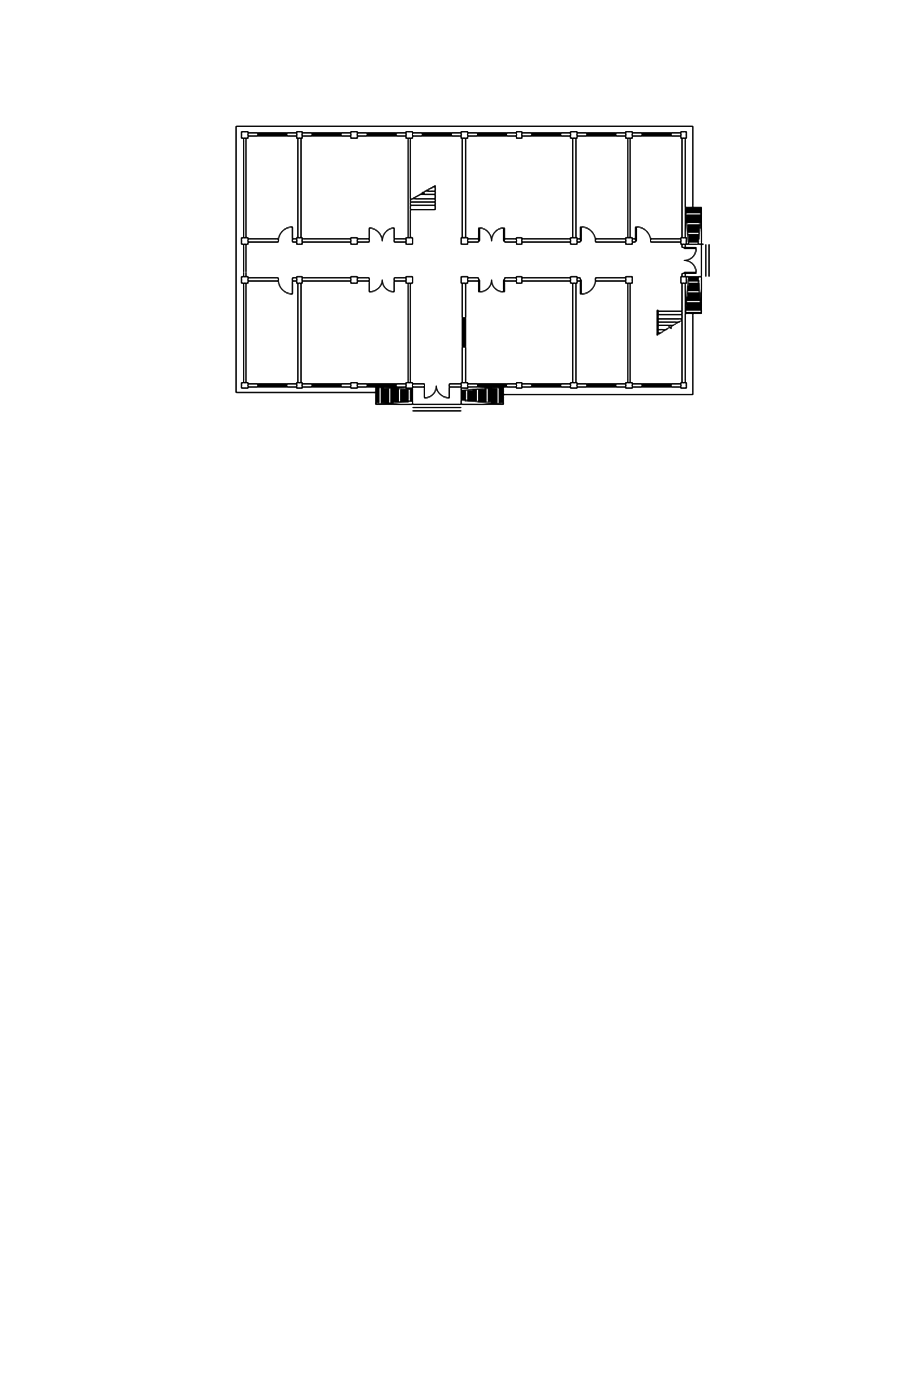
\includegraphics[width=0.9\columnwidth]{figures/2-8/2-8-1.pdf}
  \end{figure}

  \column{0.55\textwidth}
  \fsize{\textrm{in the example right, the walls of a room are separated by some arcs, lines and white squares, it is not feasible to simply extract rooms from CAD models}}

\end{columns}

\end{frame}

%------------------------------------------------

\begin{frame}
\frametitle{Problem State}

\begin{problem}[Extracting CAD Spatial Objects]
  Given a CAD model (DXF file), return a set of rooms, doors, and the topological relationship between doors and rooms, where each room is represented as a polygon, each door is represented as a point, and each topological relationship is a pair of (door, room) indicating that a door is connected with a room.
\end{problem}

\end{frame}

%------------------------------------------------

\begin{frame}
\frametitle{The Proposed Method: Basic Idea}

\textbf{DOORS}~~As doors are usually represented by arcs, just simply extract all arcs as door candidates and further make a refinement to remove those candidates that are not connected with rooms (after rooms have been recognized)\\~\\

\textbf{ROOMS}~~A rule-based approach is used, considering the following two problems: 1. a room's wall may involve too many lines in CAD models; 2. rooms are not always rectangles and they may be more than one door associated.\\~\\

\textbf{BASIC IDEA}~~to first employ a line-reduction preprocessing to simplify the line set that composed of a room; after that, use a line-extending technique to divide the entire indoor space into a set of geometric shapes; finally, use an MBR-based method to remove duplicated rooms.

\end{frame}

%------------------------------------------------

\begin{frame}
\frametitle{The Proposed Method: Definitions}

\begin{definition}[point-point adjacency]
  Two points are adjacent if their Euclidean distance is below a predefined threshold $\alpha$
  \begin{equation}
    p \overset{adj}{\leftrightarrow} q \Leftrightarrow dist(p,q) \leq \alpha
  \end{equation}
\end{definition}

\begin{definition}[point-line adjacency]
  A point $p$ is adjacent to a line $ln(s,e)$ if there is a \emph{point-point adjacency} relation between $ln$'s start point or end point and $p$
  \begin{equation}
    p \overset{adj}{\leftrightarrow} ln \Leftrightarrow (p \overset{adj}{\leftrightarrow} s \textbf ~or~ p \overset{adj}{\leftrightarrow} s)
  \end{equation}
\end{definition}

\end{frame}

%------------------------------------------------

\begin{frame}
\frametitle{The Proposed Method: Difinitions}

\begin{definition}[line-line adjacency]
  Let $ln_1(s_1, e_1)$ and $ln_2(s_2, e_2)$ be two lines. $ln_1$ and $ln_2$ are adjancent if there is a \emph{point-line adjacency} relation between an end point of one of the two lines and another line.
  \begin{equation}
    ln_1 \overset{adj}{\leftrightarrow} ln_2 \Leftrightarrow (s_1 \overset{adj}{\leftrightarrow} ln_2 ~or~e_1 \overset{adj}{\leftrightarrow} ln_2) ~or~ (s_2 \overset{adj}{\leftrightarrow} ln_1 ~or~e_2 \overset{adj}{\leftrightarrow} ln_1)
  \end{equation}
\end{definition}

\begin{definition}[parallel lines]
  Let $ln_1(s_1, e_1)$ and $ln_2(s_2, e_2)$ be two lines. $ln_1$ and $ln_2$ are parallel such that they satisfy the following condition.
  \begin{equation}
    ln_1 \overset{par}{\leftrightarrow} ln_2 \Leftrightarrow dot\_product(ln_1, ln_2) - dist(s_1, e_1) \cdot dist(s_2,e_2) < \beta
  \end{equation}
\end{definition}

\end{frame}

%------------------------------------------------

\begin{frame}
\frametitle{The Proposed Method: Difinitions}

Distance between two lines are computed as follows
\begin{figure}[tb]
  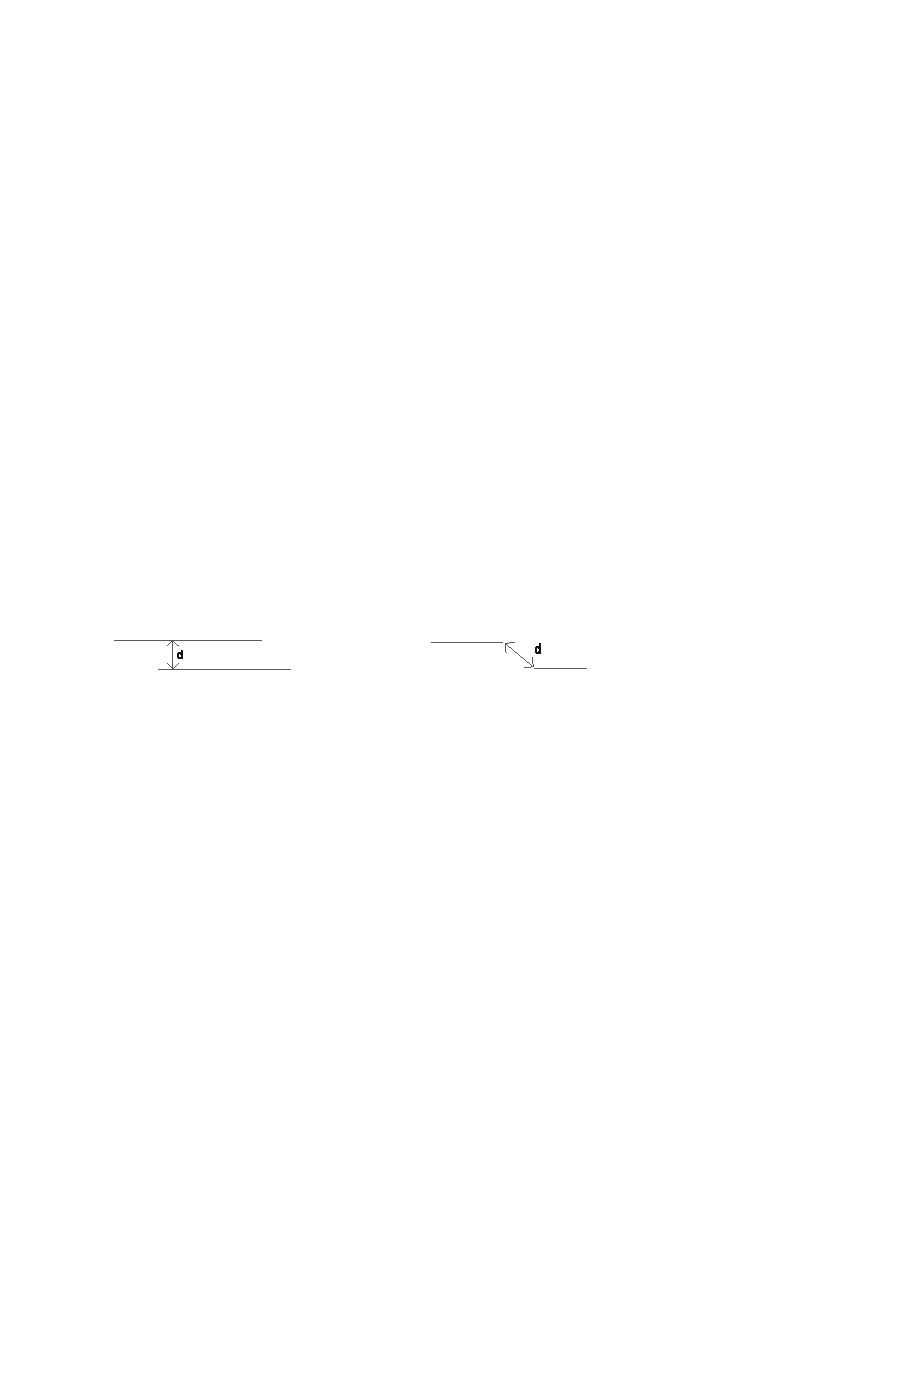
\includegraphics[width=\columnwidth]{figures/2-8/2-8-2.pdf}
\end{figure}

\begin{definition}[near lines]
  Two parallel lines are near if the distance between them is below a predefined threshold $\varepsilon$
\end{definition}

\end{frame}

%------------------------------------------------

\begin{frame}
\frametitle{The Proposed Method: Algorithm}

\begin{columns}

  \column{0.58\textwidth}
  \begin{figure}[tb]
    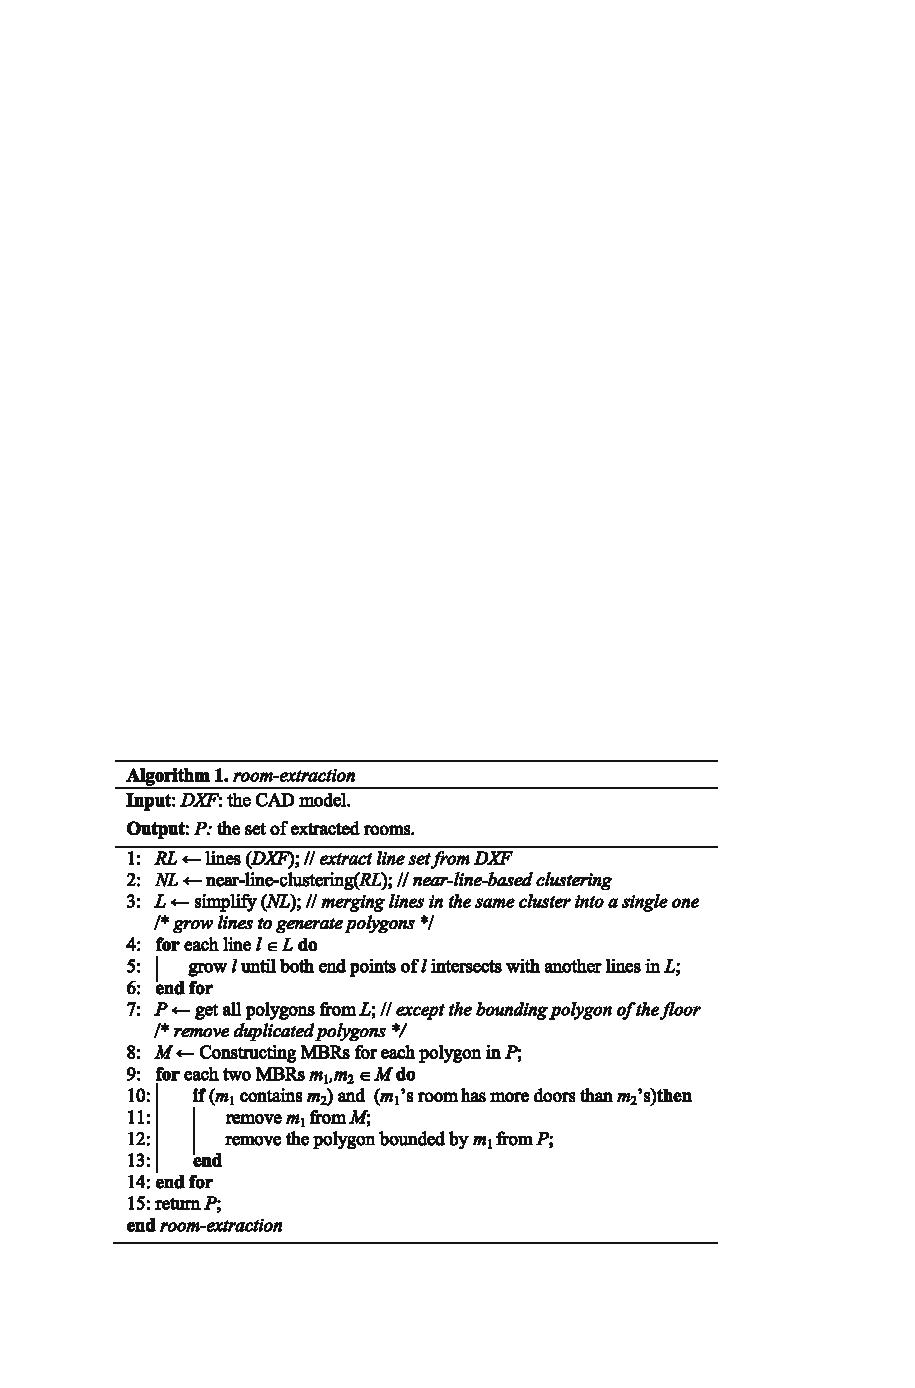
\includegraphics[width=\columnwidth]{figures/2-8/2-8-3.pdf}
  \end{figure}


  \column{0.42\textwidth}
  \ssize{
  \begin{enumerate}
    \item first obtain line clusters through a near-line-based clustering step
    \item simplify the lines in each cluster by merging near lines into a single line
    \item construct polygons using a line-growing technique, and then remove duplicated polygons by constructing MBRs for all polygons
    \item after extracting rooms, continue to refine door candidates that are extracted from arcs in the CAD model
    \item those candidates not connected with any rooms are removed from the door set.
  \end{enumerate}
  }

\end{columns}

\end{frame}

%------------------------------------------------

\begin{frame}
\frametitle{Integration into Indoor Moving-Object Databases}

Current relational database systems do not provide inherited support for complex object representation and storage. \\~\\

Object-relational database systems such as Oracle and PostgreSQL offer user-defined type extensions. \\~\\

Three indoor spatial types on Oracle, which are \emph{Indoor Position}, \emph{Indoor Space}, \emph{Indoor Geometry}. Oracle Spatial provides \emph{SDO\_GEOMETRY} for representing spatial data.

\end{frame}

%------------------------------------------------

\begin{frame}
\frametitle{Integration into Indoor Moving-Object Databases}

\textbf{Indoor Space} type describes rooms, doors, as well as the topological relationship between doors and rooms, representing as a tripe $(RoomSet, DoorSet, Room-Door)$. Where $RoomSet$ is the set of room identifiers, $DoorSet$ is the set of door identifiers, and $Room-Door$ represents the topological relationship between $RoomSet$ and $DoorSet$.\\~\\

\textbf{Indoor Geometry} type stores the exact geometric information about rooms and doors with the form $(ObjectID, Geo)$, where $ObjectID$ is a room ID or a door ID and $Geo$ is an \emph{SDO\_GEOMETRY} type supported by Oracle Spatial.

\end{frame}

% %------------------------------------------------

\begin{frame}[allowframebreaks]
\frametitle{References}

\begin{thebibliography}{99} % Beamer does not support BibTeX so references must be inserted manually as below
\bibliographystyle{abbrv}
\fsize{

\bibitem{xu2015extracting}
D.~Xu, P.~Jin, X.~Zhang, J.~Du, and L.~Yue.
\newblock Extracting Indoor Spatial Objects from CAD Models: A Database Approach.
\newblock In {\em Database Systems for Advanced Applications}, pp. 273--279, 2015.

\bibitem{autoc77:online}
\url{http://images.autodesk.com/adsk/files/autocad_2012_pdf_dxf-reference_enu.pdf}.
\newblock DXF Reference (2012).
\newblock Accessed on 05/12/2016.

}
\end{thebibliography}

\end{frame}


%------------------------------------------------
\section{3. Indoor Data Cleansing} % Sections can be created in order to organize your presentation into discrete blocks, all sections and subsections are automatically printed in the table of contents as an overview of the talk
%------------------------------------------------

\subsection{3.1 Leveraging Spatio-Temporal Redundancy for RFID Data Cleansing} % A subsection can be created just before a set of slides with a common theme to further break down your presentation into chunks

% \begin{frame}
\frametitle{About This Work...}

\emph{Leveraging Spatio-Temporal Redundancy for RFID Data Cleansing}.~\cite{chen2010leveraging} \\
H.~Chen, W-S.~Ku, H.~W and M-T.~S.\\~\\

\begin{itemize}
  \item Published at \emph{SIGMOD' 2010}.
  \item Proposed a Bayesian inference based approach for cleaning RFID raw data.
  \item Desined an $n$-state detection model to capture the likelihood.
  \item Devised a Metropolis-Hastings sampler with Constraints (MH-C) to sample from the posterior.
\end{itemize}

\end{frame}

%------------------------------------------------

\begin{frame}
\frametitle{Motivation}

To take full advantage of:

\begin{itemize}
  \item duplicate readings (by multiple readers simultaneously or by a single reader over a period of time) of the same object are very common.
  \item prior knowledge about the readers and the environment (e.g., prior data distribution, false negative rates of readers) may help improve data quality and remove data anomalies.
  \item given constraints in target applications (e.g., the number of objects in a same location cannot exceed a given value).
\end{itemize}

\end{frame}

%------------------------------------------------

\begin{frame}
\frametitle{Data Redundancy: Spatial Redundancy}

\fsize{\textrm{The challenge is how to take advantage of redundancy while avoiding its undesirable effect in data cleansing.}}

\vspace{-10pt}
\begin{columns}[c]

  \column{0.5\textwidth}
  \begin{figure}[tb]
    \includegraphics[width=\columnwidth]{figures/3-1/3-1-2.pdf}
  \end{figure}

  \begin{example}
    \ssize{
    \textrm{
    the target area is divided into 6 zones, an RFID reader is located in the center of each zone. Spatial overlap of readers' detection regions leads to duplicate readings, i.e., an object is in the detection regions of multiple readers.
    }}
  \end{example}

  \column{0.5\textwidth}
  \begin{figure}[tb]
    \includegraphics[width=\columnwidth]{figures/3-1/3-1-1.pdf}
  \end{figure}

  \ssize{
  The above table shows two effects of redundancy:
  \begin{enumerate}
    \item Object 2 is detected by both readers in Zone 2 and 3, at least one of the readings belongs to spatial redundancy.
    \item Object 3 is detected in Zone 4 only, however, it does not necessarily mean that the Object 3 is in Zone 4 for sure.
  \end{enumerate}
  }

\end{columns}

\end{frame}

%------------------------------------------------

\begin{frame}
\frametitle{Data Redundancy: Temporal Redundancy}

Many applications monitor the target area using a \emph{mobile reader} instead of employing multiple \emph{stationary readers}.\\~\\

Because the exact location of the mobile reader is always changing, the detection regions at different time points may overlap.\\~\\

\textbf{The temporal redundancy problem can be reduced to the spatial redundancy problem:} by treating the same reader at different time points as different readers.

\end{frame}

%------------------------------------------------

\begin{frame}
\frametitle{Prior Knowledge}

As false negatives and false positives abound in raw RFID readings, in order to revoer the true information, the data cleasing system should take prior knowledge into account.\\~\\

For example, the detection areas of readers in Zone 2 and 3 have significant overlapping, the positioning of the reader in Zone 4 makes it more likely to detect objects in Zone 3 than objects in Zone 5, or the reader in Zone 3 has high false negative rate.

\end{frame}

%------------------------------------------------

\begin{frame}
\frametitle{Constraints}

\emph{Environmental constraints} can be utilized to improved data cleansing.\\~\\

For example, the maximal capacity of each zone (the number of objects that can reside the same zone) is a constraint.\\~\\

In addition to these pysical constraints, information obtained from other channels can be translated into constraints. E.g., if an extra source indicates that two certain objects are in the same zone, it may help cleanse the data of there two.

\end{frame}

%------------------------------------------------

\begin{frame}
\frametitle{Overview of the Approach}

\begin{enumerate}
  \item By using Bayesian inference, it derives a universal framework of computing the posterior probabilities (of the location of each object).
  \item Based on the physical characteristic of RFID readers, it proposes an $n$-state detection model to capture likelihoods.
  \item It devised MH-C, an improved \emph{Metropolis-Hastings} sampler, to sample from the posterior while taking the environmental constraints into consideration.
\end{enumerate}

\end{frame}

%------------------------------------------------

\begin{frame}
\frametitle{Notations}

\begin{figure}[tb]
  \includegraphics[width=\columnwidth]{figures/3-1/3-1-3.pdf}
\end{figure}

\end{frame}

%------------------------------------------------

\begin{frame}
\frametitle{A Bayesian Interface Base Approach}

\conceptbf{Bayesian Interface} estimates the probalility of a hypothesis $(x)$ based on observations $(y)$, showing that posterior is proportional to the multiplication of likelihood and prior, i.e., $p(x|y) \propto p(y|x)p(x)$.\\~\\\pause

Suppose there're $m$ zones (each with a reader mounted in the center) and $n$ objects. For each object $o_i$, its location is represented by a random variable $h_i$. A possible distribution of $n$ objects in $m$ zones can be denoted as an instance of the random vector:\pause
\begin{equation}
  \hat{H} = \{ h_1, h_2, ..., h_n \}
\end{equation}
\pause

where $h_i$ represents the zone ID where object $o_i$ is in. E.g., $h_1 = 2$ denotes that object $o_1$ is in zone 2 in the current instance.

\end{frame}

%------------------------------------------------

\begin{frame}
\frametitle{A Bayesian Interface Base Approach}

For the reader in zone $j$, the raw data (0 or 1) it receives from the RFID tag of objects $o_i$ is denoted as $z_{ij}$. Thr \emph{raw data matrix} for each complete scan from $m$ readers can then be represented as an $n \times m$ matrix $\mathbb{Z} = [z_{ij}]$. \\~\\ \pause

Using the \conceptbf{Bayesian theorem}, where $post(\hat{H}|\mathbb{Z})$ denotes the posterior probability of location vector $\hat{H}$ given the raw data matrix $\mathbb{Z}$. The hypothesis should satisfy all constraints: \pause
\begin{equation}
  \begin{split}
  post(\hat{H}|\mathbb{Z}) = 0 & :\hat{H} \textrm{ is not valid} \\
  post(\hat{H}|\mathbb{Z}) > 0 & :\hat{H} \textrm{ is valid} \\
  post(\hat{H_1}|\mathbb{Z}) > post(\hat{H_2}|\mathbb{Z}) & :\hat{H_1} \textrm{ is more likely than } \hat{H_2}
  \end{split}
\end{equation}

\end{frame}

% %------------------------------------------------

\begin{frame}[allowframebreaks]
\frametitle{References}

\begin{thebibliography}{99} % Beamer does not support BibTeX so references must be inserted manually as below
\bibliographystyle{abbrv}
\fsize{

\bibitem{chen2010leveraging}
H.~Chen, W-S.~Ku, H.~W and M-T.~S.
\newblock Leveraging spatio-temporal redundancy for RFID data cleansing.
\newblock In {\em SIGMOD}, pp. 51--62, 2010.

\bibitem{jeffery2006adaptive}
S.R.~Shawnm, M.~Garofalakis, M.J.~Franklin.
\newblock Adaptive cleaning for RFID data streams.
\newblock In {\em VLDB}, pp. 163--174, 2006.

\bibitem{rao2006deferred}
J.~Rao, S.~Doraiswamy, H.~Thakkar, L.S.~Latha.
\newblock A deferred cleansing method for RFID data analytics.
\newblock In {\em VLDB}, pp. 175--186, 2006.

\bibitem{andrieu2003introduction}
C.~Andrieu, N.~De~Freitas, A.~Doucet, M.I.~Jordan.
\newblock An introduction to MCMC for machine learning.
\newblock In {\em Machine learning}, pp. 5--43, 2003.

}
\end{thebibliography}

\end{frame}


\subsection{3.2 Spatiotemporal Data Cleansing for Indoor RFID Tracking Data} % A subsection can be created just before a set of slides with a common theme to further break down your presentation into chunks

% \begin{frame}
\frametitle{About This Work...}

\emph{Spatiotemporal Cleansing for Indoor RFID Tracking Data}.~\cite{baba2013spatiotemporal} \\
A.I.~Baba, H.~Lu, X.~Xie, T.B.~Pedersen\\~\\

\begin{itemize}
  \item Published at \emph{MDM' 2013}.
  \item Focused on two quality aspects in raw indoor RFID data, temporal redundancy and spatial ambiguity.
  \item Investigated the spatiotemporal characteristics of indoor spaces as well as RFID reader deployment to be exploited in cleansing.
\end{itemize}

\end{frame}

%------------------------------------------------

\begin{frame}
\frametitle{Motivation}

\begin{itemize}
  \item Effective RFID tracking data management is expected to support various applications.
  \begin{sitemize}
    \item range from monitoring to analysis of indoor moving objects
    \item RFID reader reports the object's presence to the database that manages the object positions
  \end{sitemize}
  \item However, noises and errors abound in raw data.
  \begin{sitemize}
    \item radio frequency waves are not steady and therefore the detection range may change from time to time
    \item such dirtiness hinders the progress of applying meaningful high level application.
  \end{sitemize}
  \item Cleansing RFID data is therefore needed.
\end{itemize}

\end{frame}

%------------------------------------------------

\begin{frame}
\frametitle{Dirtiness in Indoor RFID Tracking Data}

\textrm{An RFID reader report $(readerID, objectID, time)$ means the object identified by $objectID$ is seen by the reader identified by $readerID$ at time point $time$}.\\~\\

\conceptbf{Temporal Redundancy}~~~~A tagged object can be read many times by the same reader within a short period, depending on the sampling frequency configured for a reader.\\~\\

\conceptbf{Spatial Ambiguity}~~~~A tagged object can be read by multiple readers simultaneously. This may result from the unexpected change of the detection range of a reader nearby.

\end{frame}

%------------------------------------------------

\begin{frame}
\frametitle{Dirtiness in Indoor RFID Tracking Data}

\begin{figure}[tb]
  \includegraphics[width=0.6\columnwidth]{figures/3-2/3-2-1.pdf}
\end{figure}

\vspace{-15pt}
\begin{columns}

  \column{0.5\textwidth}
  \begin{example}
    \ssize{
    Two readers $r_1$, $r_2$ in two rooms respectively. Object $O_1$ moves in the left room from time point $t_1$ to time point $t_5$, which yields five reports by $r_1$ as the trajectory is within $r_1$'s detection range. If times points are very close to each other, the five reports can be compressed into a single tuple $\langle r_1, O_1, [t_1,t_5] \rangle$.
    }
  \end{example}

  \column{0.5\textwidth}
  \begin{example}
    \ssize{
    At time point $t_3$, object $O_1$ is detected by both readers. This is due to the unexpected expansion of $r_2$'s detection range. Consequently, from the RFID data, $O_1$ seems to be in both rooms at same time $t_3$. Thus spatial ambiguity is caused. By considering such spatiotemporal constraints, our cleansing technique is able to remove spatial ambiguous reports such as $\langle r_2, O_1, t_3 \rangle$.
    }
  \end{example}

\end{columns}

\end{frame}

%------------------------------------------------

\begin{frame}
\frametitle{Raw Readings Table (RRT)}

\begin{columns}[c]

  \column{0.55\textwidth}
  \begin{figure}[tb]
    \includegraphics[width=\columnwidth]{figures/3-2/3-2-2.pdf}
  \end{figure}

  \column{0.45\textwidth}
  \begin{sitemize}
    \item each raw reading is in the format of $(deviceID, objectID, t)$, which means that the object identified by $objectID$ is detected by the device identified by $deviceID$ at time $t$.
    \item usually the detection range of a positioning device is a circular region with a pre-specified radius, a positioning device continuously detects objects that are in its range, with the frequency determined by its sampling rate.
  \end{sitemize}

\end{columns}

\end{frame}

%------------------------------------------------

\begin{frame}
\frametitle{Compared with Graph Based Indoor Tracking~\cite{DBLP:conf/mdm/JensenLY09}}

This paper distinguishes itself from the work~\cite{DBLP:conf/mdm/JensenLY09} introduced in Section 2.1:

\begin{itemize}
  \item This paper considers the overlapping between different positioning devices, whereas work~\cite{DBLP:conf/mdm/JensenLY09} assumes that devices do not overlap.
  \item This paper is intended to decide where an object really is when is is seen by multiple devices, whereas work~\cite{DBLP:conf/mdm/JensenLY09} focuses on tracking the object when it is not seen by any devices.
  \item In order to support data cleansing, this paper porposes a \emph{Distance-Aware Graph} different from the \emph{Deployment Graph} introduced in Section 2.
\end{itemize}

\end{frame}

%------------------------------------------------

\begin{frame}
\frametitle{Notations}

\begin{figure}[tb]
  \includegraphics[width=\columnwidth]{figures/3-2/3-2-3.pdf}
\end{figure}

\end{frame}

%------------------------------------------------

\begin{frame}
\frametitle{Definitions and Tasks}

\begin{definition}[Temporal Redundant Readings]
  Two raw readings $rr_i$ and $rr_j$ are temporal redundant readings if $|rr_i.t - tt_j.t| \leq \tau$, $rr_i.deviceID = rr_j.deviceID$ and $rr_i.objectID = rr_j.objectID$, where $\tau$ is an application-specific threshold.
\end{definition}

\begin{definition}[Tracking Record]
  Given a series of temporal redundant readings $rr_1, ..., rr_k$, a tracking record $tr$ is a temporal aggregation of them. Formally, $tr$ is in the format $(deviceID, objectID, t_s, t_e)$, where $tr.deviceID = rr_i.deviceID$, $tr.objectID = rr_i.objectID$, $tr.t_s = rr_1.t$ and $tr.t_e = tt_k.t$ for $1 \leq i \leq k$.
\end{definition}

\end{frame}

%------------------------------------------------

\begin{frame}
\frametitle{Definitions and Tasks}

\begin{definition}[Spatial Ambiguous Tracking Records]
  Two tracking records $tr'$ and $tr$ are spatial ambiguous if $tr'.deviceID \neq tr.deviceID$ and $tr'.objectID = tr.objectID$, if $tr'.[t_s, t_e] \cap tr.[t_s, t_e] \neq \varnothing $, or if $tr.t_s - tr'.t_e \leq min\_tt$, where $min\_tt$ is the minimum travelling time for an object to move from $tr'$'s device to $tr$'s device.
\end{definition}

\end{frame}

%------------------------------------------------

\begin{frame}
\frametitle{Definitions and Tasks}

\begin{block}{Task (Temporal Redundancy Elimination)}
  This task is to aggregate raw readings into more meaningful tracking records. This way is expected to significantly reduce the data size without any information loss.
\end{block}

\begin{block}{Task (Spatial Ambiguity Reduction)}
  Given a large set of tracking records, this task is to identify spatial ambiguous tracking records and reduce such spatial ambiguities by referring to the spatiotemporal constrains imposed by the positioning device deployment as well as the indoor topology.
\end{block}

\textrm{these two tasks together are called \conceptbf{spatiotemporal data cleansing}}.

\end{frame}

%------------------------------------------------

\begin{frame}
\frametitle{Overview of Spatiotemporal Data Cleansing}

\begin{figure}[tb]
  \includegraphics[width=\columnwidth]{figures/3-2/3-2-4.pdf}
\end{figure}

\end{frame}

%------------------------------------------------

\begin{frame}
\frametitle{Phase 1: Temporal Cleansing}

\begin{columns}[c]

  \column{0.5\textwidth}
  \begin{figure}[tb]
    \includegraphics[width=\columnwidth]{figures/3-2/3-2-2.pdf}
  \end{figure}

  \column{0.5\textwidth}
  \begin{figure}[tb]
    \includegraphics[width=\columnwidth]{figures/3-2/3-2-5.pdf}
  \end{figure}

\end{columns}

\vspace{15pt}
\begin{sitemize}
  \item sequentially scan data from the raw reading table and generates more meaningful tracking records by aggregating on the time.
  \item the aggregation results are controlled by the threshold $\tau$.
  \item all generated tracking records are stored in the \conceptbf{Aggregate Tracking Table} (ATT).
  \item the threshold $\tau$ in the example is 4 time units.
\end{sitemize}

\end{frame}

%------------------------------------------------

\begin{frame}
\frametitle{Phase 2: Spatial Cleansing}

\begin{columns}[c]

  \column{0.5\textwidth}
  \begin{figure}[tb]
    \includegraphics[width=\columnwidth]{figures/3-2/3-2-5.pdf}
  \end{figure}

  \column{0.5\textwidth}
  \begin{figure}[tb]
    \includegraphics[width=\columnwidth]{figures/3-2/3-2-6.pdf}
  \end{figure}

\end{columns}

\vspace{10pt}
\begin{sitemize}
  \item take the aggregate tracking table as input, identify possible spatial ambiguities, and reduce them by a distance-aware graph.
  \item the distance-aware graph is constructed by all positioning devices in the indoor space.
  \item assuming the minimum movement time between device $r_6$ and $r_7$ is one unit, $object_1$'s tracking record $(r_7, object_1, t_3, t_{10})$ is truncated to $(t_7, object_1, t_8, t_{10})$.
  \item it assumes that the first tracking record in $ATT$ is correct, while it is not always true in practice.
\end{sitemize}

\end{frame}

%------------------------------------------------

\begin{frame}
\frametitle{Temporal Cleansing Algorithm}

\begin{columns}[c]

  \column{0.5\textwidth}
  \begin{figure}[tb]
    \includegraphics[width=\columnwidth]{figures/3-2/3-2-7.pdf}
  \end{figure}

  \column{0.5\textwidth}
  \begin{sitemize}
    \item Line 1: starts with the initialization of a new aggregate tracking table $ATT$.
    \item Line 4: for each raw reading $rr$ from $RRT$, all the aggregate tracking records with the same device and object as $rr$ in the current $ATT$ are fetched into set $trs$.
    \item Line 5--10: if $trs$ is not empty and $rr$ is temporally close enough to an existing tracking record $tr$ in $trs$, $tr$'s time interval is extended to $rr.t$ and $rr$ is processed.
    \item Line 11--12: otherwise, $rr$ cannot be combined to any existing tracking record, and therefore a new tracking record is created and inserted.
  \end{sitemize}

\end{columns}

\end{frame}

%------------------------------------------------

\begin{frame}
\frametitle{Temporal Cleansing Algorithm: Threshold Setting}

\begin{equation}
  Threshold(\tau) = \frac{\text{detection range diameter}}{\text{object moving speed}}
\end{equation}

\begin{figure}[tb]
  \includegraphics[width=0.7\columnwidth]{figures/3-2/3-2-8.pdf}
\end{figure}

\end{frame}

%------------------------------------------------

\begin{frame}
\frametitle{Distance-Aware Deployment Graph}

\begin{columns}[c]

  \column{0.62\textwidth}
  \ssize{
  \begin{block}{Distance-Aware Deployment Graph}
    $G_{dd} = (V,E,\mathcal{L}_V,\mathcal{L}_E)$
    \begin{sitemize}
      \item $V$ is a set of vertices, each vertex represents a deployed positioning device $r_i$;
      \item $E$ is the set of edges, where $E = \{ (r_i, r_j) | r_i, r_j \in V \wedge r_i \neq r_j \wedge D2V(r_i) \cap D2V(r_j) \neq \varnothing \}$;
      \item $\mathcal{L}_V : V \rightarrow R$ assigns to a vertex $v_i$ the minimum dwell time that an object $o$ should spend in device $r_i$'s detection range such that $o$ is detected by device $r_i$;
      \item $\mathcal{L}_E : E \rightarrow R \times R $ assigns to a edge $(r_i, r_j)$ the minimum indoor walking distance between two devices $r_i$ and $r_j$ and the maximum speed with which an object can move between them, i.e., $\mathcal{L}_E((r_i,r_j)) = (d_{i,j}, S_{i,j})$.
    \end{sitemize}
  \end{block}
  }

  \column{0.38\textwidth}
  \begin{figure}[tb]
    \includegraphics[width=\columnwidth]{figures/3-2/3-2-9.pdf}
  \end{figure}
  \ssize{\textrm{The goal of \emph{Distance-Aware Deployment Graph} is to enable deriving the minimum travel time from one reader to another.}}

\end{columns}

\end{frame}

%------------------------------------------------

\begin{frame}
\frametitle{Distance-Aware Deployment Graph Construction}

\begin{columns}[c]

  \column{0.5\textwidth}
  \begin{figure}[tb]
    \includegraphics[width=\columnwidth]{figures/3-2/3-2-10.pdf}
  \end{figure}

  \column{0.5\textwidth}
  \begin{sitemize}
    \item Lines 2--6: for each pair of device $r_i$ and $r_j$, the indoor shortest path $P$ is found if the edge $(r_i, r_j)$ is not in the graph yet;
    \item Lines 7--8: if $P$ only contains devices $r_i$ and $r_j$, a new edge is created with the corresponding weights;
    \item Lines 10--14: otherwise each pair of consecutive devices on $P$ are processed likewise.
  \end{sitemize}

\end{columns}

\end{frame}

%------------------------------------------------

\begin{frame}
\frametitle{Spatial Cleansing Algorithm}

\begin{columns}[c]

  \column{0.5\textwidth}
  \begin{figure}[tb]
    \includegraphics[width=\columnwidth]{figures/3-2/3-2-11.pdf}
  \end{figure}
  \ssize{
  \textrm{
  To identify and reduce the possible spatial ambiguity involving two RFID readers $r_s$ and $r_t$, one should first compute the minimum traveling time $(min\_tt(r_s, r_t))$ that a moving object needs to reach from $r_s$ to $r_t$.
  }
  }

  \column{0.5\textwidth}
  \begin{sitemize}
    \item Line 2: for each tracking record $tr$ in $ATT$, check its dwell time $tr.t_e - tr.t_s$;
    \item Line 3: get $tr$'s previous tracking record $tr'$ from $ATT$ that involves the same object and device as $tr$;
    \item Line 6: get the minimum traveling time from $tr'.deviceID$ and $tr.deviceID$;
    \item Line 7: if the idle time between $tr'$ and $tr$ is too short compared to the minimum traveling time plus the minimum dwell time for $tr.deviceID$;
    \item Line 8: truncate $tr.t_s$ accordingly to make sure the idle time is sufficient with respect to the spatiotemporal constraints;
    \item Lines 9--10: delete $tr$ from $ATT$ if its updated dwell time is too short.
  \end{sitemize}

\end{columns}

\end{frame}

%------------------------------------------------

\begin{frame}
\frametitle{Cases of Spatial Cleansing}

\begin{figure}[tb]
  \includegraphics[width=\columnwidth]{figures/3-2/3-2-12.pdf}
\end{figure}

\begin{sitemize}
  \item Case(a): the idle time between two consecutive tracking records is sufficiently long, i.e., longer than the minimum traveling time between devices $r_6$ and $r_7$;
  \item Case(b): it is need to truncate $tr.[t_s, t_e]$, cutting $tr$'s part shown in black, because the idle time between $tr'$ and $tr$ is too short;
  \item Case(c): $tr$ is deleted after the spatial cleansing because its remaining dwell time is too short.
\end{sitemize}

\end{frame}

%------------------------------------------------

\begin{frame}
\frametitle{Conclusions}



It designs a temporal cleansing algorithm to aggregate raw RFID readings temporally such that the data size is compressed without information loss.\\~\\

It designs a spaital cleansing technique: proposing a distance-aware deployment graph to capture the spatiotemporal constrains implied by the deployment of RFID readers as well as the indoor topology.\\~\\

The techniques proposed in this paper also apply to indoor tracking data obtained by other symbolic positioning technologies, like Bluetooth.


\end{frame}

% %------------------------------------------------

\begin{frame}[allowframebreaks]
\frametitle{References}

\begin{thebibliography}{99} % Beamer does not support BibTeX so references must be inserted manually as below
\bibliographystyle{abbrv}
\fsize{

\bibitem{baba2013spatiotemporal}
A.I.~Baba, H.~Lu, X.~Xie, T.B.~Pedersen.
\newblock Spatiotemporal data cleansing for indoor RFID tracking data.
\newblock In {\em MDM}, pp. 187--196, 2013.

\bibitem{chen2010leveraging}
H.~Chen, W-S.~Ku, H.~Wang, M-T.~Sun.
\newblock Leveraging spatio-temporal redundancy for RFID data cleansing.
\newblock In {\em SIGMOD}, pp. 51--62, 2010.

\bibitem{DBLP:conf/mdm/JensenLY09}
C.S.~Jensen, H.~Lu, B.~Yang.
\newblock Graph model based indoor tracking.
\newblock In {\em {MDM}}, pp. 122--131, 2009.

}
\end{thebibliography}

\end{frame}


\subsection{3.3 Handling False Negatives in Indoor RFID Data} % A subsection can be created just before a set of slides with a common theme to further break down your presentation into chunks

% \begin{frame}
\frametitle{About This Work...}

\emph{A Graph Model for False Negative Handling in Indoor RFID Tracking Data}.~\cite{baba2013graph} \\
A.I.~Baba, H.~Lu, T.B.~Pedersen, X.~Xie\\~\\

\begin{itemize}
  \item Published at \emph{SIGSPAITAL' 2013}.
  \item Focuses on handling \emph{false negatives} which occur when a moving object passes the detection range of an RFID reader but the reader fails to produce any readings.
  \item Proposes the transition probabilities that capture how likely objects move from one RFID reader to another.
\end{itemize}

\end{frame}

%------------------------------------------------

\begin{frame}
\frametitle{Motivation}

\begin{itemize}
  \item RFID emerges to be one of the key technologies to modernize object tracking and monitoring systems in indoor environments.
  \begin{sitemize}
    \item airport baggage tracking
  \end{sitemize}
  \item However, the unreliable nature of raw data captured by readers is a major factor hindering the development of various applications.
  \begin{sitemize}
    \item loss and error rate can be between 30-40\%.~\cite{floerkemeier2004issues}
    \item read events are frequently missed due to the detection ability of a reader, the quality of an RFID tag, and constraints of the environment.~\cite{derakhshan2007rfid}
  \end{sitemize}
  \item Critical to cleanse the RFID raw data, and provide clean data to high level applications to make correct interpretations and analysis of the physical world.
\end{itemize}

\end{frame}

%------------------------------------------------

\begin{frame}
\frametitle{False Negatives}

\begin{figure}[tb]
  \includegraphics[width=0.8\columnwidth]{figures/3-3/3-3-1.pdf}
\end{figure}
\vspace{-10pt}
\begin{example}
  \ssize{
  two readers $r_1$ and $r_2$ in one hall and $r_3$ in another hall. Object $O_1$ enters the hall at time $t_1$ and is continuously tracked by $r_1$ until $t_3$. After that, $O_1$ is detected by $r_3$ at $t_7$ and $r_3$ keeps tracking $O_1$ until $t_9$. However, $O_1$ is not supposed to be detected by $r_3$ before it's detected by reader $r_2$ on its way, because to enter into the hall where $r_3$ is, $O_1$ must pass the detection range of $r_1$ and $r_2$ and cannot remain undetected for time interval $[t_3, t_7]$.
  }
\end{example}

\end{frame}

%------------------------------------------------

\begin{frame}
\frametitle{Aggregate Tracking Table (ATT)~\cite{baba2013spatiotemporal}}

\begin{itemize}

  \item All raw readings are ordered by their detection times and are aggregated into tracking records in \conceptbf{Aggregate Tracking Table}($ATT$).

  \item Each generated tracking record is in the format of $(deviceID, objectID, t_s, t_e, r_{Count})$.

  \item The meaning is that object identified by $objectID$ is detected by device identified by $deviceID$ during time interval $[t_s, t_e]$ for $r_{Count}$ times.
\end{itemize}

\end{frame}

%------------------------------------------------

\begin{frame}
\frametitle{Definitions}

\begin{definition}[False Negatives]
  Given a reader $r_i$ and a moving object $O$, if object $O$ goes through the detection range of reader $r_i$ during time interval $[t, t']$, but $r_i$ does not generate any reading about $O$'s presence during time interval $[t, t']$, a false negative occurs in the data.
\end{definition}

\begin{definition}[False Negatives Handling]
  Given an $ATT$, the false negative handling process detects false negatives and inserts recovered tracking records into the $ATT$.
\end{definition}

\end{frame}

%------------------------------------------------

\begin{frame}
\frametitle{Transition Probabilities}

\conceptbf{Markov Property}: each step a move to next reader (vertice) only depends on current reader and not the readers that precede it, holding a ``memorylessness''.\\~\\ \pause

A moving object at reader $r_i$ moves to a neighboring reader $r_j$ with a probability proportional to the probability weight of the edge $(r_i, r_j)$, i.e., the probability of a transition from $r_i$ to neighboring $r_j$ is : \pause
\begin{equation}
  \frac{p(r_i, p_j)}{\sum_{k \in N(r_i)}p(r_i, K)}
\end{equation}

\pause
Here, $N(r_i)$ is the set of neighbors of reader $r_i$. The transitional probability $p(r_i, r_j)$ denotes the probability that a moving object is detected by $r_j$ at some time later after $t$ given that it was detected by $r_i$ at time $t$ without any third reader involved in-between.

\end{frame}

%------------------------------------------------

\begin{frame}
\frametitle{Transition Probabilities}

\begin{definition}[Transition]
  A transition takes place when a moving object moves from a reader $r_i$ to another reader $r_j$ without passing through any intermediate readers.
\end{definition}

\vspace{10pt}

\conceptbf{A transition probability matrix} represents the transition relationship between a finite number of readers:
\begin{equation}
  P = \begin{bmatrix}
p(r_1, r_1) & p(r_1, r_2) & \cdots & p(r_1, r_n)\\
p(r_2, r_1) & p(r_2, r_2) & \cdots & p(r_2, r_n)\\
\vdots & \vdots & \vdots & \vdots\\
p(r_n, r_1) & p(r_n, r_2) & \cdots & p(r_n, r_n)
\end{bmatrix}
\end{equation}

\vspace{5pt}

For each deployed reader $r_i$, $\sum_{j=1}^{n}p(p_i,p_j) = 1$.

\end{frame}

%------------------------------------------------

\begin{frame}
\frametitle{Transition Probabilities}

The elements of the transition matrix $P$ are then obtained as follows:

\vspace{10pt}

\begin{equation}
  p(r_i, p_j) = \left\{\begin{matrix}
\frac{N_{ij}}{N_i} & \text{if}~(r_i, r_j) \in G_{pdm}.E\\
0 & \text{otherwise}
\end{matrix}\right.
\end{equation}

\vspace{10pt}

where $N_{ij}$ is the number of objects moving from $r_i$ to $r_j$, $N_i$ is the total number of objects moving from $r_i$, $G_{pdm}$ is a probabilistic distance-aware graph model.

\end{frame}

%------------------------------------------------

\begin{frame}
\frametitle{Probabilistic Distance-Aware Graph Model}

\begin{block}{Probabilistic Distance-Aware Graph Model}
  $G_{pdm} = (V, E, \mathcal{L}_V, \mathcal{L}_E)$
  \begin{fitemize}
    \item $V$ is a set of vertices, each represents a deployed device $r_i$.
    \item $E$ is the set of edges, where $E = \{ (r_i, r_j) | r_i, r _j \in V \cup r_i \neq r_j \}$, one can move from $r_i$ to $r_j$ without being detected by third reader.
    \item $\mathcal{L}_V: V \rightarrow \mathcal{R} \times \mathcal{R}$ assigns to a vertex $v_i$ a minimum dwell time and sampling frequency of a corresponding reader $r_i$, i.e., $mathcal{L}_V(r_i) = (d_t, S_f)$.
    \item $\mathcal{L}_E: E \rightarrow \mathcal{R} \times \mathcal{R}$ assigns to an edge $(r_i, r_j)$ the minimum indoor walking time between two devices $r_i$ and $r_j$ and the probability with which an object can move between them, i.e., $mathcal{L}_E(r_i, r_j) = (t_{i,j}, p_{r_i,r_j})$.
  \end{fitemize}
\end{block}

\end{frame}

%------------------------------------------------

\begin{frame}
\frametitle{Probabilistic Distance-Aware Graph Model}

\begin{columns}

  \column{0.6\textwidth}
  \begin{figure}[tb]
    \includegraphics[width=\columnwidth]{figures/3-3/3-3-2.pdf}
  \end{figure}

  \column{0.4\textwidth}
  \begin{fitemize}
    \item the graph is enhanced from a distance deployment graph proposed in \cite{baba2013spatiotemporal}.
    \item different readers usually imply different minimum dwell times for detection and different sampling rates.
    \item the probability weight between two readers will be used to predict the most likely path an object may have taken.
  \end{fitemize}

\end{columns}

\end{frame}

%------------------------------------------------

\begin{frame}
\frametitle{Probabilistic Distance-Aware Graph Construction}

\begin{columns}

  \column{0.55\textwidth}
  \begin{figure}[tb]
    \includegraphics[width=\columnwidth]{figures/3-3/3-3-3.pdf}
  \end{figure}

  \column{0.45\textwidth}
  \begin{enumerate}
    \ssize{
    \item lines 2--6: the indoor shortest path $sp$ is found if the edge $(r_i, r_j)$ is not in the graph yet.
    \item lines 7--9: if $sp$ only contains readers $r_i$ and $r_j$, a new edge is created with the corresponding weights.
    \item lines 11-16: otherwise, each pair of consecutive readers on $sp$ are processed likewise.
    \item indoor shortest paths are computed according to the algorithms in \cite{DBLP:conf/icde/LuCJ12}.
    }
  \end{enumerate}

\end{columns}

\end{frame}

%------------------------------------------------

\begin{frame}
\frametitle{Handling False Negatives}

\begin{definition}[Path]
  A path is a sequence of readers $r_1, r_2, ..., r_n$ where there is an edge connecting $r_i$ and $r_{r+1}$ for $i = 1, 2,...,n$. A path is simple if all $r_i$ are distinct.
\end{definition}

\begin{definition}[Candidate Path]
  Given a source reader $R_s$ and a destination reader $R_d$, a path from $R_s$ to $R_d$, represented as $R_s \overset{\delta}{\rightsquigarrow} R_d$ is a candidate path, if a path $\delta$ satisfies the spatio-temporal constraints captured by a graph.
\end{definition}

\end{frame}

%------------------------------------------------

\begin{frame}
\frametitle{Handling False Negatives}

\begin{definition}[Most Likely Path]
  Given a set of candidate path $\{ \delta_m \}_{m=1}^n$, a most likely path is:
  \begin{equation}
    \delta^* = {\arg\max}_m \prod_{E_{ij} \in \delta_m} p_{i,j}
  \end{equation}
\end{definition}

A two-phase solution is designed to handle false negatives in indoor tracking data, \emph{detecting false negatives} and \emph{recovering false negatives}.

\end{frame}

%------------------------------------------------

\begin{frame}
\frametitle{Detecting False Negatives}

\begin{itemize}

  \item take aggregated tracking table $ATT$ as an input, identifies possible false negatives using the probabilistic distance-aware graph model of all deployed readers.

  \item look at each tracking record $tr$ in $ATT$ and find out the neighbors of $tr.deviceID$.

  \item take next tracking record $tr'$ and check if $tr'.deviceID$ is in a list of neighbors of $tr.deviceID$.

  \item if none of neighbors matches, it can be concluded that one or more readers between the two devices have failed to detect a moving object with identity $tr.objectID$.

  \item find the path between the two devices using the above definitions.

\end{itemize}

\end{frame}

%------------------------------------------------

\begin{frame}
\frametitle{Recovering False Negatives}

\begin{itemize}

  \item retrieve a path between source reader $R_s$(tr.deviceID) and destination reader $R_d$(tr'.deviceID) in the graph and fills the missing readings of each reader a path contains between $R_s$ and $R_d$.

  \item the path retrieved is the most likely path, in a set of paths which satisfy the spatio-temporal constraints of subgraph between $R_s$ and $R_d$.

  \item to fill the missing readings, the parameters like, minimum travelling time between readers, minimum dwell time and sampling rate of corresponding reader are used.

  \item the approximate number of raw readings to be filled for each reader is determined as $\frac{\text{minimum dwell time}}{\text{sampling rate}}$.

\end{itemize}

\end{frame}

%------------------------------------------------

\begin{frame}
\frametitle{Conclusion}

This paper studies data cleansing for indoor RFID tracking data.\\~\\

It focuses one of the main aspects in raw indoor RFID tracking data, namely, \emph{false negatives}.\\~\\

A probabilistic distance-aware graph model is proposed to capture probabilities together with the spatio-temporal constraints implied by the deployment of RFID readers as well as indoor topology.\\~\\

The transition probabilities that capture likely an object move from one reader to another are obtained from the existing data.

\end{frame}

% %------------------------------------------------

\begin{frame}[allowframebreaks]
\frametitle{References}

\begin{thebibliography}{99} % Beamer does not support BibTeX so references must be inserted manually as below
\bibliographystyle{abbrv}
\fsize{

\bibitem{baba2013spatiotemporal}
A.I.~Baba, H.~Lu, X.~Xie, T.B.~Pedersen.
\newblock Spatiotemporal data cleansing for indoor RFID tracking data.
\newblock In {\em MDM}, pp. 187--196, 2013.

\bibitem{baba2013graph}
A.I.~Baba, H.~Lu, T.B.~Pedersen, X.~Xie.
\newblock A graph model for false negative handling in indoor RFID tracking data.
\newblock In {\em SIGSPATIAL}, pp. 464--467, 2013.

\bibitem{floerkemeier2004issues}
C.~Floerkemeier, M.~Lampe.
\newblock Issues with RFID usage in ubiquitous computing applications.
\newblock In {\em Pervasive Computing}, pp. 188--193, 2004.

\bibitem{derakhshan2007rfid}
R.~Derakhshan, M.E.~Orlowska, X.~Li.
\newblock RFID data management: challenges and opportunities.
\newblock In {\em IEEE International conference on RFID}, vol. 10, 2007.

\bibitem{DBLP:conf/icde/LuCJ12}
H.~Lu, X.~Cao, and C.~S. Jensen.
\newblock A foundation for efficient indoor distance-aware query processing.
\newblock In {\em ICDE}, pp. 438--449, 2012.

\bibitem{baba2014handling}
A.I.~Baba, H.~Lu, T.B.~Pedersen, X.~Xie.
\newblock Handling false negatives in indoor RFID data.
\newblock In {\em MDM}, pp. 117--126, 2014.

}
\end{thebibliography}

\end{frame}


\subsection{3.4 Offline Cleaning of RFID Trajectory Data (PART I)} % A subsection can be created just before a set of slides with a common theme to further break down your presentation into chunks

% \begin{frame}
\frametitle{About This Work...}

\emph{Cleaning Trajectory Data of RFID-monitored Objects through Conditioning under Integrity}~\cite{DBLP:conf/edbt/FazzingaFFP14}\\
B.~Fazzinga, S.~Flesca, F.~Furfaro, F.~Parisi.\\~\\

% \emph{Handling False Negatives in Indoor RFID Data}.~\cite{baba2014handling} \\
% A.I.~Baba, H.~Lu, T.B.~Pedersen, X.~Xie\\~\\

\begin{itemize}
  \item Published at \emph{EDBT' 2014}. %, \emph{MDM' 2014}.
  \item A probabilistic framework is introduced for reducing the inherent uncertainty of trajectory data collected for RFID-monitored objects.
  \item The framework cleans trajectories by conditioning them to the event that integrity constraints encoding some knowledge about the map and the motility characteristics of the monitored objects hold.
\end{itemize}

\end{frame}

%------------------------------------------------

\begin{frame}
\frametitle{Motivation}

\begin{itemize}
  \item Pervasive use of RFID devices as a support for object tracking
  \begin{fitemize}
    \item monitoring of people, animals and objects inside museums, schools, hospital etc.
    \item context-aware information.
  \end{fitemize}
  \item There exists ambiguity in the raw RFID data.
  \begin{fitemize}
    \item no one-to-one correspondence between locations and readers, no way to deterministically decide the location given that a set of readers detected an object.
    \item the same location may constrain different reader's detection zones, the same reader may detect different objects at different locations, also false negatives.
  \end{fitemize}
\end{itemize}

\end{frame}

%------------------------------------------------

\begin{frame}
\frametitle{Ambiguity of RFID Data}

\begin{columns}

  \column{0.4\textwidth}
  \begin{figure}[tb]
    \includegraphics[width=\columnwidth]{figures/3-4/3-4-1.pdf}
  \end{figure}

  \column{0.6\textwidth}
  \begin{example}
    \fsize{
    an object $o$ was detected at some instant by both reader $r_1$ and $r_5$, two locations are possible, $L_1$ and $L_4$. Analogously, if $o$ was detected by $r_3$ only, we cannot conclude that it was surely in $L_3$, as it could be the case that $r_2$ failed to detect it despite it was close enough to its antenna.
    }
  \end{example}

  \ssize{\textrm{\\this suggests that the association readers/locations can be naturally modeled in probabilistic terms. For instance by a probability distribution $p^a(l|R)$ defined for each location $l$ and set $R$ of readers.}}
  $p^a(L_1|\{r_1, r_5\}) = p^a(L_4|\{r_1, r_5\}) = 0.5$
  $p^a(L_0|\{r_0\}) = 1$

\end{columns}

\end{frame}

%------------------------------------------------

\begin{frame}
\frametitle{Ambiguity of RFID Data}

\begin{columns}

  \column{0.4\textwidth}
  \begin{figure}[tb]
    \includegraphics[width=\columnwidth]{figures/3-4/3-4-1.pdf}
  \end{figure}

  \column{0.6\textwidth}
  \ssize{\textrm{things become more complex when trying to translate a sequence of readings into possible trajectories, a naive way is to consider the steps of the trajectory independent from each other.}}

  \begin{example}
    \ssize{
    assume that at instants(timestamps) 0 and 1, $o$ is detected by both $r_1$ and $r_5$, while at instant 2 it's detected by $r_0$. Assume that $p^a(l|R)$ is used, i.e., objects detected by $r_1$ and $r_5$ are at location $L_1$ with probability 0.5 and at $L_4$ with probability 0.5, detected by $r_0$ are at $L_0$ with probability 1. Reasoning only on the basis of these probabilities and exploiting no further knowledge, the trajectories followed by $o$ can be: $t_1: L_1L_1L_0$, $t_2: L_1L_4L_0$, $t_3: L_4L_1L_0$, $t_4: L_4L_4L_0$, each with probability 0.25.
    }
  \end{example}

\end{columns}

\end{frame}

%------------------------------------------------

\begin{frame}
\frametitle{Ambiguity of RFID Data}

The independence assumption allows for reasoning about trajectory probabilities as follows.\\~\\
\pause

Consider an object $o$ moving over time interval $\mathcal{T} = [\tau_1,...,\tau_n]$, and the sequence of readings $\Theta = \langle \tau_1, R_1 \rangle, ..., \langle \tau_n, R_n \rangle$, meaning that at each $\tau_i \in \mathcal{T}$, $o$ was detected by the set $R_i$ of readers.\\~\\
\pause

The probability that $o$ followed the trajectory $t = l_1, ..., l_n$ can be expressed (under the independence assumption) as $p^a(t|\Theta) = \prod_{i=1}^n p^a(l_i|R_i)$.\\~\\
\pause

Unfortunately, the probabilities returned by $p^a(t|\Theta)$ can be very different from those returned by the ``actual'' probability distribution $Pr(t|\Theta)$ as the following example.

\end{frame}

%------------------------------------------------

\begin{frame}
\frametitle{Ambiguity of RFID Data}

\begin{columns}

  \column{0.4\textwidth}
  \begin{figure}[tb]
    \includegraphics[width=\columnwidth]{figures/3-4/3-4-1.pdf}
  \end{figure}

  \column{0.6\textwidth}

  \begin{example}
    \ssize{
    For the four possible trajectories $t_1: L_1L_1L_0$, $t_2: L_1L_4L_0$, $t_3: L_4L_1L_0$, $t_4: L_4L_4L_0$, we can infer only $t_1$ is the only correct interpretation of the data according to the map. Since $L_0$ and $L_4$ have no direct connection, and $L_1$ is directly connected to $L_0$ by not to $L_4$. Thus a correct probability distribution over the possible trajectories is at follows: $Pr(t_1|\Theta) = 1$, $Pr(t_2|\Theta) = Pr(t_3|\Theta) = Pr(t_4|\Theta) = 0$, where $\Theta = \theta_1, \theta_2$, and $\theta_1 = \langle \tau_1, \{ r_1, r_5 \} \rangle $, $\theta_2 = \langle \tau_2, \{ r_0 \} \rangle $.
    }
  \end{example}

  \ssize{\textrm{the point is that even $p^a(l|R)$(also $p^a(t|\Theta)$) is easy to obtain, finding a formulation for $Pr(t|\Theta)$ is very hard, as it requires analyzing and encoding the correlations among possible positions over time.}}

\end{columns}

\end{frame}

%------------------------------------------------

\begin{frame}
\frametitle{Target of This Work}

\begin{problem}
  given a sequence of readings $\Theta$ and exploiting the knowledge of $p^a(l|R)$ (and thus $p^a(t|\Theta)$), how can we effectively and efficiently revise $p^a(t|\Theta)$ so that it takes into account possible correlations inside the data, thus obtaining a better estimate of $Pr(t|\Theta)$.
\end{problem}

Intuitively enough, revising $p^a(t|\Theta)$ according to the known correlations can be viewed as a cleansing problem: the data to be cleaned are the (probabilistic) trajectories resulting from using $p^a(t|\Theta)$ to interpret the sequence of readings, and the cleansing task consists in revising the probablitisties assigned to these trajectories.

\end{frame}

%------------------------------------------------

\begin{frame}
\frametitle{Cleansing RFID Data}

Exploiting the knowledge on the map and on the motility characteristics:\\~\\

\conceptbf{Direct-unreachability Constraint} can be naturally derived on the connectivity between pairs of locations.\\~\\

\conceptbf{Traveling-time Constraint} can be derived on the time needed for reaching a location starting from another one.

\end{frame}

%------------------------------------------------

\begin{frame}
\frametitle{Cleansing RFID Data}

\begin{columns}

  \column{0.4\textwidth}
  \begin{figure}[tb]
    \includegraphics[width=\columnwidth]{figures/3-4/3-4-1.pdf}
  \end{figure}

  \column{0.6\textwidth}

  \begin{example}
    \ssize{
      the map easily implies a set of direct-unreachability constraints, one for each pair of rooms which are not directly connected through a door, such as $L_0,L_4$ and $L_1,L_4$.\\
      The map implies further constraints, other than direct unreachability. E.g., it says that $L_0$ and $L_5$, although close to one another, are connected only by a pretty long path. Reasonably, it can be imposed that $15 sec$ are required to go through this path. (called ``traveling-time constraint'').
    }
  \end{example}
  \ssize{\textrm{the above example explains how considering integrity constraints can reduce uncertainty, as it allows trajectories to be removed from the valid interpretations of data.}}

\end{columns}

\end{frame}

%------------------------------------------------

\begin{frame}
\frametitle{Cleansing RFID Data}

\fsize{

\conceptbf{The target of this work} becomes how to reasonably combine the integrity constraints with the \emph{a-priori} probabilistic model encoded by $p^a(l|R)$, in order to devise a mechanism for revising the a-priori probabilities of the remaining valid trajectories and making them sum up to 1.\\~\\

A rigorous approach~\cite{koch2008conditioning,flesca2014consistency} is to perform \conceptbf{conditioning}: starting from the a-priori probabilities(without constraints), the probabilities of the trajectories are re-evaluated as conditioned to the event that the constraints are satisfied.\\~\\

That is, given a set $\mathcal{IC}$ constraints, probabilities of the form $p^a(t|\Theta)$ are revised into $p^a(t|\Theta \wedge \mathcal{IC})$. This way, the probability of invalid trajectories becomes 0, while that of each valid trajectory becomes the ratio of its a-priori probability to the overall a-priori probability of the valid trajectories.

}

\end{frame}

%------------------------------------------------

\begin{frame}
\frametitle{Preliminaries}

\ssize{
\begin{table}
    \begin{center}
    \begin{tabular}{|c|c|}
    \hline
        \textbf{Notation} &   \textbf{Meaning}                    \\
    \hline
        $o$      &   a single object equipped with RFID tag        \\
    \hline
        $\mathcal{R} = \{ r_1, ..., r_k \}$      &   a set of RFID readers     \\
    \hline
        $\mathcal{L} = \{ l_1, ..., l_n \}$      &  the set of locations       \\
    \hline
        $\mathcal{T} = [0..\tau_f]$      &  the time interval over monitoring       \\
    \hline
        $\theta = \langle \tau, R \rangle$      &  a reading of $o$ \\
    \hline
        $\Theta$        &   a set of readings, a \emph{reading sequence} (r-sequence) \\
    \hline
        $p^a(l|R)$        &   the \emph{a-priori} probability  \\
    \hline
        $X_{\theta}$        &   the discrete random variable \\
    \hline
        $f(X_{\theta} = l) = p^a(l|\theta[readers])$        &   probability density funtion for the random variable \\
    \hline
    \end{tabular}
    \end{center}
\end{table}
}

\end{frame}

%------------------------------------------------

\begin{frame}
\frametitle{Preliminaries}

\begin{definition}[probabilistic location sequence (l-sequence)]
  given $p^a(l|R)$ and an r-sequence $\Theta$, we define the \emph{probabilistic location sequence} corresponding to $\Theta$ (according to $p^a(l|R)$) as the set $\Gamma = \{ X_{\theta} | \theta \in \Theta \}$.
\end{definition}

\fsize{
The l-sequence $\Gamma$ corresponding to the r-sequence $\Theta$ for $o$ over $\mathcal{T}$ will be denoted as a pair $\Gamma = \langle \Lambda,p \rangle$.
\begin{itemize}
  \item $\Lambda$ is a set of pairs of the form $\Lambda = \langle \tau, l \rangle$, with $\tau \in \mathcal{T}$ and $l \in \mathcal{L}$, containing at least one pair $\langle \tau, l \rangle$ for each $\tau \in \mathcal{T}$.
  \item $p$ assigns to each pair $\langle \tau, l \rangle \in \Lambda$ the value $f(X_{\theta} = l)$, where $\theta$ is the reading at time $\tau$, i.e., $p$ assigns to $\langle \tau, l \rangle$ the probability that the object was at location $l$ at time $\tau$, as implied by the PDF of the random variable.
\end{itemize}
}

\end{frame}

%------------------------------------------------

\begin{frame}
\frametitle{Preliminaries}

\begin{columns}

  \column{0.4\textwidth}
  \begin{figure}[tb]
    \includegraphics[width=\columnwidth]{figures/3-4/3-4-2.pdf}
  \end{figure}

  \column{0.6\textwidth}

  \begin{example}
    \ssize{
      consider the r-sequence $\Theta = \{ \langle 0, \{ r_1 \} \rangle, \langle 1, \{ r_2 \} \rangle, \langle 2, \{ r_4 \} \rangle \}$ and $p^a(l|R)$ s.t. $p^a(L_1|\{r_1\}) = \frac{6}{10}$, $p^a(L_2|\{r_1\}) = \frac{4}{10}$, $p^a(L_3|\{r_2\}) = \frac{1}{3}$, $p^a(L_4|\{r_2\}) = \frac{2}{3}$, $p^a(L_3|\{r_4\}) = \frac{2}{3}$, $p^a(L_5|\{r_4\}) = \frac{1}{3}$. The corresponding l-sequence $ \Gamma = \langle \Lambda, p \rangle $ is s.t. $ \Lambda = \{ \lambda_1 = \langle 0, L_1 \rangle, \lambda_2 = \langle 0, L_2 \rangle, \lambda_3 = \langle 1, L_3 \rangle, \lambda_4 = \langle 1, L_4 \rangle, \lambda_5 = \langle 2, L_3 \rangle, \lambda_6 = \langle 2, L_5 \rangle \} $, and $p(\lambda_1) = \frac{6}{10}$, $p(\lambda_2) = \frac{4}{10}$, $p(\lambda_3) = \frac{1}{3}$, $p(\lambda_4) = \frac{2}{3}$, $p(\lambda_5) = \frac{2}{3}$, $p(\lambda_6) = \frac{1}{3}$.
    }
  \end{example}

\end{columns}

\end{frame}

%------------------------------------------------

\begin{frame}
\frametitle{Preliminaries}

given a pair $\lambda = \langle \tau, l \rangle \in \Lambda$, denote the first and the second component of $\lambda$ with $\lambda[time]$ and $\lambda[loc]$ respectively.

\begin{definition}[Trajectory]
  Let $\Theta$ be an r-sequence over $\mathcal{T}$ and $\Gamma = \langle \Lambda,p \rangle$ be the l-sequence corresponding to $\Theta$. A trajectory over $\Gamma$ is a set $t \subseteq \Lambda$ of pairs such that, for each $\tau \in \mathcal{T}$, there is a unique pair $\lambda \in t$ such that $\lambda[time] = \tau$. The (a-priori) probablitity of $t$ is $p^a(t|\Theta) = \prod_{\lambda \in t}p(\lambda)$. For simplicity, we write $p^a(t|\Theta)$ as $p^a(t)$.
\end{definition}

The set of the trajectories over an l-sequence $\Gamma$ is denoted as $T(\Gamma)$. Given a trajectory $t$, the pair $\lambda \in t$ such that $\lambda[time] = \tau$ is said to be the $\tau$-th \emph{step} of $t$.

\end{frame}

%------------------------------------------------

\begin{frame}
\frametitle{Preliminaries}

\begin{columns}

  \column{0.4\textwidth}
  \begin{figure}[tb]
    \includegraphics[width=\columnwidth]{figures/3-4/3-4-2.pdf}
  \end{figure}

  \column{0.6\textwidth}

  \begin{example}
    \ssize{
      2 out of the 8 trajectories over the l-sequence $\mathcal{T} = \langle \Lambda,p \rangle$ are $t_1 = \{\lambda_1, \lambda_3, \lambda_5\}$, which means that object $o$ went from $L_1$ to $L_3$ and stayed in $L_3$ for two consecutive timestamps, and $t_2 = \{\lambda_1, \lambda_3, \lambda_6\}$, which describes the case that object $o$ went from $L_1$ to $L_5$ through $L_3$. Their a-priori probabilities are $p^a(t_1) = p(\lambda_1) \cdot p(\lambda_3) \cdot p(\lambda_5) = \frac{12}{90}$, and $p^a(t_2) = p(\lambda_1) \cdot p(\lambda_3) \cdot p(\lambda_6) = \frac{6}{90}$.

    }
  \end{example}

\end{columns}

\end{frame}

%------------------------------------------------

\begin{frame}[allowframebreaks]
\frametitle{Constraints}

\begin{definition}[Direct Unreachability (DU) Constraint]
  Given two locations $l_1, l_2 \in \mathcal{L}$, a \emph{direct unreachability} constraint has the form $unreachable(l_1,l_2)$ and states that no object can reach $l_2$ from $_1$ in one time point.
\end{definition}

\begin{definition}[Traveling Time (TT) Constraint]
  Given two locations $l_1, l_2 \in \mathcal{L}$ and a non-negative integer $\nu$, a \emph{traveling time} constraint is of the form $travelingTime(l_1, l_2, \nu)$ and states that, for any object, the time needed to move from $l_1$ to $l_2$ is not less that $\nu$.
\end{definition}

\begin{definition}[Latency (LT) Constraint]
  Given a location $l \in \mathcal{L}$ and a non-negative integer $\delta$, a \emph{latency constraint} associated with $l$ is denoted as $latency(l,\delta)$ and imposes that every time an object goes into location $l$, it must stay in $l$ for at least $\delta$ time points.
\end{definition}

\vspace{15pt}
\fsize{\textrm{$DU$ constraints are implied by the structure of the map, and $TT$ constraints are implied by the minimum distances between the locations and the maximum speed of the objects. As regards latenct constraints, they take into account the physical inertia of objects, as well as the processing times (for doing some job).}}

\end{frame}

%------------------------------------------------

\begin{frame}
\frametitle{Integrity Constraints}

\begin{definition}[Integrity Constraints]
  Let $\Gamma = \langle \Lambda, p \rangle$ be an l-sequence and $\mathcal{IC}$ a set of \emph{integrity constraints}. A trajectory $t$ over $\Gamma$ is valid w.r.t $\mathcal{IC}$ iff
  \begin{itemize}

    \item for each $latency(l, \delta) \in \mathcal{IC}$, it holds that, for each pair $\langle \tau,l \rangle$ in $t$ such that either $\tau = 0$ or there is $\langle \tau-1, l' \rangle \in t$, with $l' \neq l$, $t$ contains all the pairs $\langle \tau+i,l \rangle$ with $i \in [1...\delta-1]$;

    \item for each $unreachable(l_1, l_2) \in \mathcal{IC}$, there are no pairs $\langle \tau,l_1 \rangle$ and $\langle \tau+1,l_2 \rangle$ in $t$;

    \item for each $travelingTime(l_1, l_2, \nu)$ in $\mathcal{IC}$, there are no $\langle \tau_1, l_1 \rangle$ and $\langle \tau_2, l_2 \rangle$ in $t$, with $\tau_1 < \tau_2$, such that $\tau_2 - \tau_1 < \nu$.

  \end{itemize}
\end{definition}

\textrm{The subset of $T(\Gamma)$ containing all and only the trajectories which are valid w.r.t $\mathcal{IC}$ will be denoted as $T^{\models\mathcal{IC}}(\Gamma)$.}

\end{frame}

%------------------------------------------------

\begin{frame}
\frametitle{Integrity Constraints}

\begin{columns}

  \column{0.4\textwidth}
  \begin{figure}[tb]
    \includegraphics[width=\columnwidth]{figures/3-4/3-4-2.pdf}
  \end{figure}

  \column{0.6\textwidth}

  \begin{example}
    \ssize{
      Consider $\Gamma = \langle \Lambda,p \rangle$ and $\mathcal{IC} = \{$ $latency(L_4,2)$,$unreachable(L_2, L_3)$, $travelingTime(L_1,L_5,3) \}$, imposing that (i) if object o reaches location $L_4$, it must stay there for at least two consecutive timestamps; (ii) object $o$ cannot directly reach location $L_3$ from location $L_2$; and (iii) object $o$ cannot reach location $L_5$ from location $L_1$ in less than 3 timestamps.
    }
  \end{example}

\end{columns}

\vspace{10pt}

\fsize{\textrm{Recalling $ \Lambda = \{ \lambda_1 = \langle 0, L_1 \rangle, \lambda_2 = \langle 0, L_2 \rangle, \lambda_3 = \langle 1, L_3 \rangle, \lambda_4 = \langle 1, L_4 \rangle, \lambda_5 = \langle 2, L_3 \rangle, \lambda_6 = \langle 2, L_5 \rangle \} $, $t_1 = \{\lambda_1, \lambda_3, \lambda_5\}$ and $t_2 = \{\lambda_1, \lambda_3, \lambda_6\}$. $t_1$ is valid, as it does not violate any constraint in $\mathcal{IC}$. $t_2$ is not valid, as it does not satisfy $travelingTime(L_1, L_5, 3)$. Indeed, the difference between the timestamp of $\lambda_6$ and $\lambda_1$ is 2. It is easy to see that $t_1$ is the unique valid trajectory over $\Gamma$ and $\mathcal{IC}$.}}

\end{frame}

%------------------------------------------------

\begin{frame}
\frametitle{Maximum Traveling Time}

\begin{definition}[Maximum Traveling Time]
  Given a set $\mathcal{IC}$ of integrity constraints and a location $l \in \mathcal{L}$, we define $maxTravelingTime(l) = \max\{ \nu | travelingTime(l,l',\nu) \in \mathcal{IC} \}$, i.e., $maxTraveling(l)$ is the maximum among the minimum traveling times required for object $o$ to move from $l$ to any other $l' \in \mathcal{L}$ according to the constraints in $\mathcal{IC}$.
\end{definition}

\end{frame}

%------------------------------------------------

\begin{frame}
\frametitle{Conditioning}

\conceptbf{Conditioning}: starting from the a-priori probabilities, the probabilities of the trajectories are evaluated as conditioned to the event that the constraints are satisfied.\\~\\

\textrm{The probability of invalid trajectories becomes 0, while that of each valid trajectory becomes the ratio of its a-priori probability to the overall a-priori probability of the valid trajecories.}

\begin{block}{}
  Given a trajectory $t \in T(\Gamma)$, its probability $p^a(t)$ conditioned to the fact that the constraints in $\mathcal{IC}$ are satisfied is given by $p^a(t|\mathcal{IC})$, where:

  \begin{itemize}
    \item $p^a(t|\mathcal{IC}) = 0$ if $t$ is not valid w.r.t $\mathcal{IC}$;
    \item $p^a(t|\mathcal{IC}) = \frac{p^a(t)}{\sum_{t' \in T^{\models \mathcal{IC}}(\Gamma)} p^a(t')}$, otherwise.
  \end{itemize}

\end{block}

\end{frame}

%------------------------------------------------

\begin{frame}
\frametitle{Conditioned Trajectory Graphs}

The \conceptbf{conditioned trajectory graph} (ct-graph) over an l-sequence $\Gamma = \langle \Lambda,p \rangle$ will be exploited to concisely represent trajectories over $\Gamma$ in the presence of integrity constraints.\\~\\

The nodes of a ct-graph are said to be \emph{location nodes}, each location node $n$ corresponds to a pair $\langle \tau,l \rangle \in \Lambda$ and is connected through directed edges to location nodes (chosen among the set of \emph{successors} of $n$) corresponding to subsequent timestamps.

\end{frame}

%------------------------------------------------

\begin{frame}
\frametitle{Location Nodes}

\begin{definition}[Location Nodes]
  Given an l-sequence $\Gamma = \langle \Lambda,p \rangle$ for an object $o$ and a set $\mathcal{IC}$ of integrity constraints, a location node $n$ is a tuple of the form $\langle \tau, l, \delta, TL \rangle$, where $\langle \tau, l \rangle \in \Lambda$, $\delta \in \mathcal{T} \cup \{ \perp \}$ (where $\perp$ means ``non-specified''), and $TL$ is a (possible empty) set of pairs $\langle \tau_1, l_1 \rangle \in \Lambda$ (with $l_1 \neq l$) containing no two pairs conceding in either the timestamp or the location. It represents the following facts:
  \begin{enumerate}
    \item A. $o$ was in location $l$ at time $\tau$;
    \item B. the stay of $o$ at $l$ started $\delta$ time points before $\tau$;
    \item C. for each $\langle \tau_1, l_1 \rangle \in TL$, the most recent detection of $o$ at location $l_1$ (before $\tau$) is at time point $\tau_1$.
  \end{enumerate}
\end{definition}

\end{frame}

%------------------------------------------------

\begin{frame}
\frametitle{Location Nodes}

Given a location node $n = \langle \tau, l, \delta, TL \rangle$ and a trajectory $t$ over $\Gamma$, we say that $t$ \conceptbf{is compatible with} $n$ if, according to $t$, the facts A,B,C holds.\\~\\

E.g., both the trajectories $t_1 = \{ \langle 0,L_1 \rangle, \langle 1,L_3 \rangle, \langle 2,L_3 \rangle \}$ and $t_2 = \{ \langle 0,L_1 \rangle, \langle 1,L_3 \rangle, \langle 2,L_5 \rangle \}$ are compatible with location node $\langle 1, L_3, 0, \{ \langle 0, L_1 \rangle \} \rangle$.

\end{frame}

%------------------------------------------------

\begin{frame}
\frametitle{Location Nodes}

The information stored in a location node $n$ can be used to state that some trajectories are invalid. Specifically, any $t \in T(\Gamma)$ compatible with $n$ is invalid if either i) or ii) hold:

\begin{block}{}
  \fsize{
  i) All the following conditions are satisfied:
  \begin{itemize}
    \item $n.TL$ contains a pair $\langle \tau', l' \rangle$;
    \item there is $travelingTime(l', l'', \nu') \in \mathcal{IC}$ with $(n.\tau+1) - \tau' < \nu'$;
    \item the $(\tau+1)$-th step of $t$ is at location $l''$.
  \end{itemize}
  In fact, $t$ would represent that the object went from $l'$ to $l''$ in less than $\nu'$ time points, thus violating the $TT$ constraints.\\~\\

  ii) There is $latency(l, \delta') \in \mathcal{IC}$ with $n.\delta < \delta'$, and the $(\tau+1)$-step of $t$ is at a location different from $l$. In fact, $t$ would represent that the object went away from $l$ after staying less than $\delta'$ time points, thus violating the latency constraint.
  }
\end{block}

\end{frame}

%------------------------------------------------

\begin{frame}
\frametitle{Location Nodes}

\fsize{
E.g., consider location node $n = \{ \langle 1, L_3, 0, \{ \langle 0, L_1 \rangle \} \rangle \}$ and the $TT$ constraint $travelingTime(L_1, L_5, 3)$. It is easy to see that the information stored in $n$ can be used to state that any trajectory compatible with $n$ and whose second step is at $L_5$ is invalid. (would not reach location $L_5$ from $L_1$ in less than 3 timestamps).\\~\\

Point i) means that an entry $\langle \tau',l' \rangle$ in $n.TL$ can be used only to check $TT$ constraints involving location $l'$. Point ii) means that the value of $n.\delta$ is useful only to check latency constraints defined over $l$.\\~\\

$\mathcal{N}$ is denoted as the set of the location nodes that can be defined over $\Gamma$ and $\mathcal{IC}$. $SN$ AND $TN$ is the subsets of $\mathcal{N}$ as the \emph{source} and \emph{target} nodes (location nodes whose timestamps are the first and the last time points of $\mathcal{T}$), respectively.
}


\end{frame}

%------------------------------------------------

\begin{frame}
\frametitle{Location Nodes}

\begin{columns}

  \column{0.4\textwidth}
  \begin{figure}[tb]
    \includegraphics[width=\columnwidth]{figures/3-4/3-4-2.pdf}
  \end{figure}

  \column{0.6\textwidth}

  \begin{example}
    \ssize{
      Consider the set $\mathcal{N}$ over $\Gamma$ and $\mathcal{IC}$ consists of the following location nodes:\\
      $n_0 = \langle 0, L_1, \perp, \varnothing \rangle$, $n_1 = \langle 0, L_2, \perp, \varnothing \rangle$ \\
      $n_2 = \langle 1, L_3, \perp, \varnothing \rangle$, $n_3 = \langle 1, L_3, \perp, \{ \langle 0, L_1 \rangle \} \rangle$ \\
      $n_4 = \langle 1, L_4, 0, \varnothing \rangle$, $n_5 = \langle 1, L_4, 0, \{ \langle 0, L_1 \rangle \} \rangle$ \\
      $n_6 = \langle 2, L_3, \perp, \varnothing \rangle$, $n_7 = \langle 2, L_3, \perp, \{ \langle 0, L_1 \rangle \} \rangle$ \\
      $n_8 = \langle 2, L_5, \perp, \varnothing \rangle$, $n_9 = \langle 2, L_5, \perp, \{ \langle 0, L_1 \rangle \} \rangle$
    }
  \end{example}

\end{columns}

\end{frame}

%------------------------------------------------

\begin{frame}
\frametitle{Location Nodes}

\LARGE
$$n_2 = \langle 1, L_3, \perp, \varnothing \rangle$$

\vspace{10pt}

\fsize{
Location node $n_2$ means that:

\begin{fitemize}

  \item since $n_2.\tau = 1$ and $n_2.l = L_3$, $o$ was in $L_3$ at timestamp 1;

  \item since $n_2.\delta = \perp$, either there is no $LT$ constraint over $L_3$, or its stay at $L_3$ started more than $\delta^*$ time points before 1, where $latency(L_3, \delta^*)$ is the $LT$ constraint over $L_3$;

  \item since $n_2.TL = \varnothing$, for every location $l$ visited by the object in the past, either there is no $TT$ constraints having $l$ as the first argument, or the object left $l$ more than $\nu^*$ time points ago, where all the $TT$ constraints $travelingTime(l,l',\nu) \in \mathcal{IC}$ having $l$ as first argument are such that $\nu < \nu^*$.

\end{fitemize}

}

\end{frame}

%------------------------------------------------

\begin{frame}
\frametitle{Location Nodes}

\LARGE
$$n_5 = \langle 1, L_4, 0, \{ \langle 0, L_1 \rangle \} \rangle$$

\vspace{10pt}

\fsize{
Location node $n_5$ means that:

\begin{fitemize}

  \item $o$ was in $L_4$ at timestamp 1;

  \item its stay at $L_4$ started in the current timestamp;

  \item in the past, it stayed at $L_1$, from which it moved away at time point 0.

\end{fitemize}

}

\end{frame}

%------------------------------------------------

\begin{frame}
\frametitle{Successors of a Location Node}

\ssize{
\begin{definition}[Successor]
  Given a pair of location nodes $n_1 = \langle \tau_1, l_1, \delta_1, TL_1 \rangle$ and $n_2 = \langle \tau_2, l_2, \delta_2, TL_2 \rangle$, $n_2$ is successor of $n_1$ iff the following conditions hold:
  \begin{itemize}
    \item $\tau_2 = \tau_1 + 1$;
    \item $unreachable(l_1, l_2) \notin \mathcal{IC}$;
    \item if $l_1 = l_2$, then $\delta_2 = \delta_1 + 1$  (override ``+'': $\perp + 1 = \perp$; $x+1 = \perp$);
    \item if $l_1 \neq l_2$, and $latency(l_1, \delta) \in \mathcal{IC}$, then $\delta_1 \leq \delta$ (if $\delta_1 \neq \perp$) and either $\delta_2 = 0$ (if there is a latency constraint on $l_2$ in $\mathcal{IC}$) or $\delta_2 = \perp$ (otherwise);
    \item there is no pair $(\tau', l') \in TL_1$ such that there is a constraint $travelingTime(l',l_2,\nu)$ in $\mathcal{IC}$ with $\tau_2 - \tau' < \nu$;
    \item $TL_2 = TL_1 \cup \{ \langle \tau_1,l_1 \rangle | travelingTime(l_1,l,\delta) \in \mathcal{IC} \} \setminus$ $(\{ \langle \tau,l \rangle \in TL_1 | \tau_2 - \tau \leq maxTravelingTime(l) \} \cup \{ \langle \tau,l \rangle \in TL_1 | l = l_2 \})$
  \end{itemize}
\end{definition}
}
\end{frame}

%------------------------------------------------

\begin{frame}
\frametitle{Successors of a Location Node}

$n_2$ is a successor of $n_1$ iff:

\begin{fitemize}
  \item $n_1$ and $n_2$ refer to consecutive time points;
  \item $l_2$ can be directly reached starting from $l_1$;
  \item if at time $\tau_2$ the object is still in $l_2 = l_1$, then this is consistently reflected by an increment of $\delta_2$;
  \item no stay constraint in $\mathcal{IC}$ involving $l_1$ is violated if the object moves from $l_1$ to another location $l_2$ at time $\tau_2$;
  \item no traveling time constraint in $\mathcal{IC}$ imposing that the time needed to move from a location belonging to $TL_1$ to $l_2$ is violated if the object moves from $l_1$ to another location $l_2$ at time $\tau_2$;
  \item $TL_2$ can be obtained by first augmenting $TL_1$ with the pair $\langle \tau_1, l_1 \rangle$ (this happens if there is a traveling time constraint involving $l_1$ as the first argument), and discarding those pairs of $TL_1$ which have become useless for checking $TT$ constraint and those referring to a previous stay at $l_2$.
\end{fitemize}

\end{frame}

%------------------------------------------------

\begin{frame}
\frametitle{Successors of a Location Node}

\begin{center}
  $n_0 = \langle 0, L_1, \perp, \varnothing \rangle$, $n_1 = \langle 0, L_2, \perp, \varnothing \rangle$ \\
  $n_2 = \langle 1, L_3, \perp, \varnothing \rangle$, $n_3 = \langle 1, L_3, \perp, \{ \langle 0, L_1 \rangle \} \rangle$ \\
  $n_4 = \langle 1, L_4, 0, \varnothing \rangle$, $n_5 = \langle 1, L_4, 0, \{ \langle 0, L_1 \rangle \} \rangle$ \\
  $n_6 = \langle 2, L_3, \perp, \varnothing \rangle$, $n_7 = \langle 2, L_3, \perp, \{ \langle 0, L_1 \rangle \} \rangle$ \\
  $n_8 = \langle 2, L_5, \perp, \varnothing \rangle$, $n_9 = \langle 2, L_5, \perp, \{ \langle 0, L_1 \rangle \} \rangle$
\end{center}

\begin{example}
  $n_3$ and $n_5$ are successors of $n_0$, $n_4$ is a successor of $n_1$, $n_7$ is a successor of $n_3$.\\
  $n_2$ is not a successor of $n_1$ since $unreachable(L_2,L_3) \in \mathcal{IC}$; $n_9$ is not a successor of $n_3$ since $travelingTime(L_1, L_5, 3) \in \mathcal{IC}$; $n_9$ is not a successor of $n_2$ for both $TT$ constraints and the previous stay conditions.
\end{example}


\end{frame}

%------------------------------------------------

\begin{frame}
\frametitle{Successors of a Location Node}

\textrm{The following proposition states a property that will be fundamental for understanding how cleansing algorithm exploits the notion of successor.}\\~\\

\begin{block}{Proposition}
  If a non-target location node $n$ admits no successor then every trajectory $t$ compatible with $n$ is not valid.
\end{block}

\end{frame}

%------------------------------------------------

\begin{frame}
\frametitle{CT-Graph}

\begin{definition}[CT-Graph]
  Let $\mathcal{N}$ be the set of location nodes over the l-sequence $\Gamma$, and $\mathcal{IC}$ a set of integrity constraints. A conditioned trajectory graph (ct-graph) is a tuple $G = \langle N, E, p_N, \vec{p}_E \rangle$��
  \begin{fitemize}
    \item $N \subseteq \mathcal{N}$;
    \item $\langle N,E \rangle$ is a graph (where $N$ and $E$ are the sets of nodes and edges, respectively) satisfying the following properties
      \begin{sitemize}
        \item a pair $\langle n_1, n_2 \rangle$ belongs to $E$ iff $n_1, n_2 \in N$ and $n_2$ is a successor of $n_1$;
        \item for every $n \in N$, there is at least one path from a source node to a target node in $N$ which contains $n$.
      \end{sitemize}
    \item $p_N: SN \rightarrow (0, 1]$ is a PDF over the set of source nodes;
    \item $\vec{p}_E$ is a set containing, for each non-target node $n$ of $G$, a PDF $p^n_E$ over its outgoing edges, i.e., $\vec{p}_E = \{ p^n_E | n \in N \setminus TN \}$ where $p^n_E: E_n \rightarrow (0,1]$ and $E_n = \{ \langle n, n' \rangle | \langle n, n' \rangle \in E \}$
  \end{fitemize}
\end{definition}

\end{frame}

%------------------------------------------------

\begin{frame}
\frametitle{CT-Graph}

A (valid) path $\pi$ over a ct-graph $G = \langle N,E,p_N,\vec{p}_E \rangle$ is a path from a source to a target node over the graph $\langle N,E \rangle$.\\~\\

A path $\pi = n_0, ..., n_{\tau_f}$ over $G$ corresponds to the valid trajectory $t = n_0[\lambda],...,n_{\tau_f}[\lambda]$, where $n_i[\lambda]$ denotes the $\langle timestamp, location \rangle$ pair which $n_i$ refers to.\\~\\

The functions $p_N$ and $\vec{p}_E$ is equal to the conditioned probability $p^a(t | \mathcal{IC})$ of the corresponding trajectory $t$, where
\begin{equation}
  p(\pi) = p_N(n_0) \times \prod_{i=0}^{\tau_f-1}p_E^{n_i}(\langle n_i, n_{i+1} \rangle)
\end{equation}

\end{frame}

%------------------------------------------------

\begin{frame}
\frametitle{Location Nodes}

\begin{columns}

  \column{0.4\textwidth}
  \begin{figure}[tb]
    \includegraphics[width=\columnwidth]{figures/3-4/3-4-2.pdf}
  \end{figure}

  \column{0.6\textwidth}

  \begin{example}
    \ssize{
      It is easy to check $G = \langle N,E,p_N,\vec{p}_E \rangle$, where $N = \{ n_0, n_3, n_7 \}$, $E= \{ \langle n_0,n_3 \rangle, \langle n_3,n_7 \rangle \}$, $p_N(n_0) = 1$, and $p_E^{n_3}(\langle n_3, n_7 \rangle) = 1$. $G$ is the ct-graph over the l-sequence and the constraints. In fact, the unique path $\pi = n_0, n_3, n_7$ over $G$ corresponds to the unique valid trajectory $\{ \lambda_1, \lambda_3, \lambda_5 \}$, and its probability is $p(\pi) = 1$.
    }
  \end{example}

\end{columns}

\end{frame}

%------------------------------------------------

\begin{frame}
\frametitle{The Cleansing Algorithm: Overview}

\begin{columns}

  \column{0.4\textwidth}
  \begin{figure}[tb]
    \includegraphics[width=\columnwidth]{figures/3-4/3-4-3.pdf}
  \end{figure}

  \column{0.6\textwidth}
  \begin{sitemize}
    \item consists of \emph{forward} and \emph{backward} phase;
    \item the forward phase consists of one iteration for each timestamp $\tau \in \mathcal{T}$, at the first iteration, the set $N$ of the location nodes belonging to the ct-graph $G$ being constructed is initialized with the set to those implied by the a-priori probabilities.
    \item at $\tau$-th iteration, $N$ is progressively augmented with location nodes referring to the timestamp $\tau+1$, the edges between location nodes referring to timestamp $\tau$ and their successors are added to $E$, and their probabilities are set to those implied by the a-priori probability function.
    \item the backward phase deals with removing the nodes in the invalid paths, the probabilities of edges and those of source nodes are conditioned, i.e., they are revised to take into account the probabilities of the trajectories that are invalid.
  \end{sitemize}

\end{columns}

\end{frame}

%------------------------------------------------

\begin{frame}
\frametitle{The Cleansing Algorithm: Initialization}

\begin{columns}

  \column{0.42\textwidth}
  \begin{figure}[tb]
    \includegraphics[width=\columnwidth]{figures/3-4/3-4-4.pdf}
  \end{figure}

  \column{0.58\textwidth}
  \begin{enumerate}
    \ssize{
    \item lines 1--2: the set $N$ if the nodes of graph is initialized with the set of the source nodes yielded by function \emph{sourceNodes} that builds them from the l-sequence $\Gamma$.
    \item lines 3--4: the probability $p_N(n)$ of each source node $n$ is set to the probability of the pair $\langle 0,l\rangle$ of $\Gamma$, and the queue $Q$ is set to be empty.
    }
  \end{enumerate}

\end{columns}

\begin{example}
  according to the previous example, function \emph{sourceNodes} builds the source location nodes $n_0$ and $n_1$, and puts them into $N$. Next, $p_N(n_0)$ and $p_N(n_1)$ are assigned probabilities $p(\lambda_1) = \frac{6}{10}$ and $p(\lambda_2) = \frac{4}{10}$, respectively.
\end{example}

\end{frame}

%------------------------------------------------

\begin{frame}
\frametitle{The Cleansing Algorithm: Forward Phase}

\begin{columns}

  \column{0.55\textwidth}
  \begin{figure}[tb]
    \includegraphics[width=\columnwidth]{figures/3-4/3-4-5.pdf}
  \end{figure}

  \column{0.45\textwidth}
  \begin{enumerate}
    \ssize{
    \item line 7: for each location node $n$ referring to $\tau$, \emph{buildSuccessors} returns the its successor $n'$;
    \item line 10: each node $n'$ is added to $N$ and consequently the edges of the form $\langle n, n' \rangle$ are added to the set $E$ of $G$;
    \item line 12: once all successors have been added to $G$, $n.loss$ is set to the one's complement of the sum of the probabilities of the outgoing edge of $n$.
    }
  \end{enumerate}

\end{columns}

\end{frame}

%------------------------------------------------

\begin{frame}
\frametitle{The Cleansing Algorithm: Forward Phase}

\begin{figure}[tb]
  \includegraphics[width=0.5\columnwidth]{figures/3-4/3-4-6.pdf}
\end{figure}

\vspace{-15pt}

\begin{example}
  \ssize{
  At iteration $\tau = 0$, both $n_0$ and $n_1$ are processed. In the case $n=n_0$, the inner loop processes the location nodes $n_3$ and $n_5$, both nodes $n_3$ and $n_5$ are sucessors of $n_0$, and both $\langle n_0,n_3 \rangle$ and $\langle n_0,n_5 \rangle$ are added to $E$, with probabilities $p(\langle n_0,n_3 \rangle) = p(\langle 1,L_3 \rangle) = 1/3$ and $p(\langle n_0,n_5 \rangle) = p(\langle 1,L_4 \rangle) = 2/3$. At the end of the loop, $n_0.loss$ is 0 and thus $n_0$ is not added to $Q$. \\
  Another example, $n_2$ is not a successor of $n_0$ or $n_1$, in the case $n=n_1$, the loop only processes the location node $n_4$, the probability $p(\langle n_1,n_4 \rangle) = p(\langle 1, L_4\rangle) = 1/3$, and $n_1.loss = 1 - 1/3 = 2/3$, thus $n_1$ is added to $Q$.
  }
\end{example}

\end{frame}

%------------------------------------------------

\begin{frame}
\frametitle{The Cleansing Algorithm: Forward Phase}

\begin{figure}[tb]
  \includegraphics[width=0.5\columnwidth]{figures/3-4/3-4-7.pdf}
\end{figure}

\vspace{-15pt}

\begin{example}
  \ssize{
  At iteration $\tau = 1$, $n_3$, $n_5$ and $n_4$ are processed. In the case $n = n_3$, the inner loop only processes the location node $n_7$ where is the only successor of $n_3$. Thus, $n_7$ is added to $N$, the edge $\langle n_3,n_7 \rangle$ is added to $E$, and the probability $p(\langle n_3, n_7 \rangle) = p(\langle 2, L_3 \rangle) = 2/3$. Next, $n_3.loss$ is assigned with $1 - 2/3 = 1/3$ and $n_3$ is added to $Q$.\\
  In both the cases $n = n_5$ and $n = n_4$, since there is no location node which is a successor of $n_5$ or $n_4$, $n_5.loss$ and $n_4.loss$ are both assigned with 1 and both $n_5$ and $n_4$ are added to $Q$.
  }
\end{example}

\end{frame}

%------------------------------------------------

\begin{frame}
\frametitle{The Cleansing Algorithm: Backward Phase}

\begin{columns}

  \column{0.42\textwidth}
  \begin{figure}[tb]
    \includegraphics[width=\columnwidth]{figures/3-4/3-4-8.pdf}
  \end{figure}

  \column{0.58\textwidth}
  \begin{sitemize}
    \item line 16: a node $n$ among those having the highest timestamp is extracted from $Q$;
    \item line 19: if $n.loss$ is lower than 1 (meaning that $n$ has at least one outgoing edge), the probability of each of the outgoing edges of $n$ is conditioned, i.e., its current value is divided by the sum of the probabilities of the outgoing edges of $n$;
    \item line 22: the probability of each ingoing edge $\langle n',n \rangle$ of $n$ is decremented by the value of $n.loss$ multiplied by the old probability value of the edge $\langle n',n \rangle$;
    \item line 23: the value of $n'.loss$ of each node $n'$ of which $n$ is successor is incremented of the value of $n.loss$ multiplied by the old probability value of the edge $\langle n',n \rangle$;
  \end{sitemize}

\end{columns}

\end{frame}

%------------------------------------------------

\begin{frame}
\frametitle{The Cleansing Algorithm: Backward Phase}

\begin{columns}

  \column{0.42\textwidth}
  \begin{figure}[tb]
    \includegraphics[width=\columnwidth]{figures/3-4/3-4-8.pdf}
  \end{figure}

  \column{0.58\textwidth}
  \begin{sitemize}
    \item line 25: since $n'.loss$ has been incremented and thus it is greater than 0, node $n'$ is added to $Q$ if it's not already present in it;
    \item line 27: furthermore, in the case $n.loss = 1$, the edge $\langle n',n \rangle$ is removed from $E$;
    \item line 29: at the end of the loop scanning the ingoing edges of $n$, if $n.loss = 1$, $n$ is removed from $N$;
    \item line 31: the probability $p_N(n)$ of each source node $n$ in $N$ is conditioned, i.e., $p_N(n)$ is divided by the sum of the probabilities of the source nodes belonging to $N$.
  \end{sitemize}

\end{columns}


\end{frame}

%------------------------------------------------

\begin{frame}
\frametitle{The Cleansing Algorithm: Backward Phase}

\begin{figure}[tb]
  \includegraphics[width=0.65\columnwidth]{figures/3-4/3-4-9.pdf}
\end{figure}

\vspace{-15pt}

\begin{example}
  \ssize{
  At the first iteration of the while loop, node $n_4$ is removed from $Q$ since $n_4.loss$ is equal to 1. Thus, the algorithm processes the ingoing edges of $n_4$. Specifically, as $n_4$ has only the incoming edge $\langle n_1,n_4 \rangle$, the probability value of $\langle n_1,n_4 \rangle$ is set to $2/3 -2/3 = 0$, and, correspondingly variable $n_1.loss$ is set to $1/3 + 2/3 = 1$. Then the edge $\langle n_1,n_4 \rangle$ is removed from $N$.
  }
\end{example}

\end{frame}

%------------------------------------------------

\begin{frame}
\frametitle{The Cleansing Algorithm: Backward Phase}

\begin{figure}[tb]
  \includegraphics[width=0.65\columnwidth]{figures/3-4/3-4-10.pdf}
\end{figure}

\vspace{-15pt}

\begin{example}
  \ssize{
  The second iteration of the while loop processes the node $n_5$. Since $n_5.loss$ is equal to 1, no conditioning of outgoing edges is performed. Then algorithm processes the ingoing edges of $n_5$, and, reasoning as in the case in the last slide, the probability value $\langle n_0,n_5 \rangle$ is set to 0, and variable $n_0.loss$ is set to $2/3$. Next $n_0$ is inserted into $Q$, the edge $\langle n_0,n_5 \rangle$ is removed from $N$.
  }
\end{example}

\end{frame}

%------------------------------------------------

\begin{frame}
\frametitle{The Cleansing Algorithm: Backward Phase}

\begin{figure}[tb]
  \includegraphics[width=0.65\columnwidth]{figures/3-4/3-4-11.pdf}
\end{figure}

\vspace{-15pt}

\begin{example}
  \ssize{
  At the third iteration of the while, node $n_3$ is removed from $Q$. Since $n_3.loss$ is lower than 1, the algorithm performs the conditioning of the outgoing edges of $n_3$ so that the probability of the unique outgoing edge $\langle n_3,n_7 \rangle$ of $n_3$ is set to 1. Next, the unique ingoing edge $\langle n_0,n_3 \rangle$ is scanned, the probability of $\langle n_0,n_3 \rangle$ is set to $1/3 - 1/3 \cdot 1/3 = 2/9$, and variable $n_0.loss$ is set to $2/3 + 1/3 \cdot 1/3 = 7/9$. Since $n_0$ is already in $Q$, the iteration processing $n_3$ ends without doing anything else.
  }
\end{example}

\end{frame}

%------------------------------------------------

\begin{frame}
\frametitle{The Cleansing Algorithm: Backward Phase}

\begin{figure}[tb]
  \includegraphics[width=0.8\columnwidth]{figures/3-4/3-4-12.pdf}
\end{figure}

\vspace{-15pt}

\begin{example}
  \ssize{
  At the fourth iteration of the while loop the node $n_1$ is removed from $Q$ and processed. Since $n_1.loss$ is equal to 1 and it has no ingoing edges $n_0.loss < 1$, the revising is skipped. At this stage, the probability of the source node $n_0$ (the unique that is still in $N$) is conditioned, obtaining $p_N(n_0) = 1$.
  }
\end{example}

\end{frame}

%------------------------------------------------

\begin{frame}
\frametitle{Conclusions and Future Work}

A probabilistic cleansing framework for RFID data has been introduced, which cleans trajectories by conditioning them to the event that integrity constraints encoding some knowledge about the map and the motility characteristics of the moving objects.\\~\\

Future work will be focused on extending the framework to take into account other forms of correlations, such as those holding in groups of objects moving together, which typically characterize supply-chain scenarios.

\end{frame}

% %------------------------------------------------

\begin{frame}[allowframebreaks]
\frametitle{References}

\begin{thebibliography}{99} % Beamer does not support BibTeX so references must be inserted manually as below
\bibliographystyle{abbrv}
\fsize{

\bibitem{DBLP:conf/edbt/FazzingaFFP14}
B.~Fazzinga, S.~Flesca, F.~Furfaro, F.~Parisi.
\newblock Cleaning Trajectory Data of RFID-monitored Objects through Conditioning under Integrity Constraints.
\newblock In {\em EDBT}, pp. 379--390, 2014.

\bibitem{koch2008conditioning}
C.~Koch, D.~Olteanu.
\newblock Conditioning probabilistic databases.
\newblock In {\em VLDB}, pp. 313--325, 2008.

\bibitem{flesca2014consistency}
S.~Flesca, F.~Furfaro, F.~Parisi.
\newblock Consistency checking and querying in probabilistic databases under integrity constraints.
\newblock In {\em Journal of Computer and System Sciences}, pp. 1448--1489, 2014.


% \bibitem{baba2013spatiotemporal}
% A.I.~Baba, H.~Lu, X.~Xie, T.B.~Pedersen.
% \newblock Spatiotemporal data cleansing for indoor RFID tracking data.
% \newblock In {\em MDM}, pp. 187--196, 2013.
%
% \bibitem{baba2013graph}
% A.I.~Baba, H.~Lu, T.B.~Pedersen, X.~Xie.
% \newblock A graph model for false negative handling in indoor RFID tracking data.
% \newblock In {\em SIGSPATIAL}, pp. 464--467, 2013.
%
% \bibitem{floerkemeier2004issues}
% C.~Floerkemeier, M.~Lampe.
% \newblock Issues with RFID usage in ubiquitous computing applications.
% \newblock In {\em Pervasive Computing}, pp. 188--193, 2004.
%
% \bibitem{derakhshan2007rfid}
% R.~Derakhshan, M.E.~Orlowska, X.~Li.
% \newblock RFID data management: challenges and opportunities.
% \newblock In {\em IEEE International conference on RFID}, vol. 10, 2007.
%
% \bibitem{DBLP:conf/icde/LuCJ12}
% H.~Lu, X.~Cao, and C.~S. Jensen.
% \newblock A foundation for efficient indoor distance-aware query processing.
% \newblock In {\em ICDE}, pp. 438--449, 2012.
%
% \bibitem{baba2014handling}
% A.I.~Baba, H.~Lu, T.B.~Pedersen, X.~Xie.
% \newblock Handling false negatives in indoor RFID data.
% \newblock In {\em MDM}, pp. 117--126, 2014.


}
\end{thebibliography}

\end{frame}


\subsection{3.4 Offline Cleaning of RFID Trajectory Data (PART II)} % A subsection can be created just before a set of slides with a common theme to further break down your presentation into chunks

% \begin{frame}
\frametitle{About This Work...}

\emph{Offline cleaning of RFID trajectory data}~\cite{fazzinga2014offline}\\
B.~Fazzinga, S.~Flesca, F.~Furfaro, F.~Parisi.\\~\\

\begin{itemize}
  \item Published at \emph{SSDBM' 2014}.
  \item A smoothing technique following a two-way filtering scheme that embeds a sampling strategy for efficiently dealing with missing detections.
\end{itemize}

\end{frame}

%------------------------------------------------

\begin{frame}
\frametitle{Motivation}

\begin{itemize}
  \item Pervasive use of RFID devices as a support for object tracking
  \begin{fitemize}
    \item monitoring of people, animals and objects inside museums, schools, hospital etc.
    \item context-aware information.
  \end{fitemize}
  \item There exists ambiguity in the raw RFID data.
  \begin{fitemize}
    \item no one-to-one correspondence between locations and readers, no way to deterministically decide the location given that a set of readers detected an object.
    \item the same location may constrain different reader's detection zones, the same reader may detect different objects at different locations, also false negatives.
  \end{fitemize}
\end{itemize}

\end{frame}

%------------------------------------------------

\begin{frame}
\frametitle{Ambiguity of RFID Data}

\begin{columns}

  \column{0.4\textwidth}
  \begin{figure}[tb]
    \includegraphics[width=\columnwidth]{figures/3-4/3-4-1.pdf}
  \end{figure}

  \column{0.6\textwidth}
  \begin{example}
    \fsize{
    an object $o$ was detected at some instant by both reader $r_1$ and $r_5$, two locations are possible, $L_1$ and $L_4$. Analogously, if $o$ was detected by $r_3$ only, we cannot conclude that it was surely in $L_3$, as it could be the case that $r_2$ failed to detect it despite it was close enough to its antenna.
    }
  \end{example}

  % \ssize{\textrm{\\this suggests that the association readers/locations can be naturally modeled in probabilistic terms. For instance by a probability distribution $p^a(l|R)$ defined for each location $l$ and set $R$ of readers.}}
  % $p^a(L_1|\{r_1, r_5\}) = p^a(L_4|\{r_1, r_5\}) = 0.5$
  % $p^a(L_0|\{r_0\}) = 1$

\end{columns}

\end{frame}

%------------------------------------------------

\begin{frame}
\frametitle{Ambiguity of RFID Data}

\begin{columns}

  \column{0.4\textwidth}
  \begin{figure}[tb]
    \includegraphics[width=\columnwidth]{figures/3-4/3-4-1.pdf}
  \end{figure}

  \column{0.6\textwidth}
  \begin{figure}[tb]
    \includegraphics[width=\columnwidth]{figures/3-4/3-4-13.pdf}
  \end{figure}

  \vspace{-10pt}

  \begin{example}
    \ssize{
    $t = 1$: an object detected by $r_0$ is surely at $L_0$ (since the area covered by $r_0$ is totally inside $L_0$)\\
    $t = 2$: an object detected by $r_1$ can be either at $L_1$ or $L_4$ (if object only detected by $r_1$ could also be laid in the area covered by $r_1$ and $r_5$, as $r_5$ may fail to detect the object, the false negative)\\
    $t = 3$: an object detected by no reader can be almost anywhere\\
    $t = 4$: reader $r_6$ covers portions of $L_3, L_4, L_8, L_9$ only.
    }
  \end{example}


\end{columns}

\end{frame}

%------------------------------------------------

\begin{frame}
\frametitle{Ambiguity of RFID Data}

\ssize{\textrm{assume that $o$ is a person, his maximum speed is $v_{max} = 2m/s$. Consider the size of the floor is $15m \times 11m$, re-examine the possible location as follow:}}

\vspace{10pt}

\begin{columns}

  \column{0.3\textwidth}
  \begin{figure}[tb]
    \includegraphics[width=\columnwidth]{figures/3-4/3-4-1.pdf}
  \end{figure}


  \column{0.7\textwidth}
  \ssize{
  A.  As regards $t = 2s$, $o$ must be at $L_1$, as it cannot be at $L_4$. In fact, $o$ was at $L_0$ at $t = 1s$, and the minimum (indoor) distance between $L_0$ and $L_4$ (about 7m) cannot be covered in $1sec$ without exceeding $v_{max}$. \\~\\
  B.  As regards $t = 3s$, now that it has been established that $o$ was at $L_1$ at $t = 2s$, we can restrict the set of possbile locations from $\{ L_1,...,L_{10} \}$ to $\{ L_0, L_1, L_2 \}$ (due to the size of the floor, reaching a room not in this set from any position inside $L_1$ in one second would require a speed greater than $v_{max}$). \\~\\
  C.  As regards $t = 4s$, the only location in $\{ L_3, L_4, L_8, L_9 \}$ (the set of location covered by $r_6$) that can be reached from at least one location in $\{ L_0, L_1, L_2 \}$ (the possible locations at time $t = 3s$, as established at point B) is $L_4$.
  }


\end{columns}

\end{frame}

%------------------------------------------------

\begin{frame}
\frametitle{Ambiguity of RFID Data}

\ssize{\textrm{all the arguments used in Point A,B,C show that the exploiting the correlation with the past positions can reduce (or even eliminate) the uncertainty in determining the position at any time point. Trying to further reduce the uncertainty by exploiting the correlation:}}

\vspace{10pt}

\begin{columns}

  \column{0.3\textwidth}
  \begin{figure}[tb]
    \includegraphics[width=\columnwidth]{figures/3-4/3-4-1.pdf}
  \end{figure}


  \column{0.7\textwidth}
  \ssize{
  D.  Consider $t = 3s$, we have already established that the position of $o$ at the subsequent time point is $L_4$, and that the possible locations for this time point are $L_0, L_1, L_2$. Hence, at $t = 3s$, $o$ must have been at $L_2$, as this is the only among the possible locations for this time point from which $L_4$ can be reached in one second without exceeding $v_{max}$.
  }

  \begin{figure}[tb]
    \includegraphics[width=\columnwidth]{figures/3-4/3-4-14.pdf}
  \end{figure}


\end{columns}

\end{frame}

%------------------------------------------------

\begin{frame}
\frametitle{The Problem Setting for This Work}

\fsize{

An instance of \conceptbf{smoothing problem}~\cite{smith2013sequential}: estimating the state of an observed entity at a time point $t \in [1...T]$ on the basis of all the observations over $[1...T]$ in terms of a posterior probability distribution over the possible states.\\~\\

This work proposes a smoothing technique following a two-way-filtering scheme that embeds a sampling strategy for efficiently dealing with missing detections.\\~\\

In the first \emph{forward} phase, time points are processed from the first to the last, and the possible positions at each time point are filtered by taking into account the results of the previous steps.\\~\\

In the \emph{backward} phase, it proceeds from the last to the first time point: for each time point, filter the positions detected as admissible in the forward phase and revise their weights, by checking whether they are a valid position when looking at the results obtained for the future time point.

}

\end{frame}

%------------------------------------------------

\begin{frame}
\frametitle{The Problem Setting for This Work}

\fsize{

The map of the locations is assumed to be partitioned according to a grid, thus the positions to be filtered and weighted at each step of the forward phase are the grid cells compatible with the readers that performed the detection.\\~\\

Thus, the grid cells may result in too many candidate positions, a variant of the cleaning algorithm where missing detections are treated by integrating the grid-based approach with sampling strategy is proposed.\\~\\

At the end of each forward step involving a missing detection, the cells that survived the filtering are further filtered according to a sampling technique, where the probability of a cell to be sampled is an estimate of the probability it would have been assigned if it was considered also in the following phases.

}

\end{frame}

%------------------------------------------------

\begin{frame}
\frametitle{The Preliminaries}

\begin{figure}[tb]
  \includegraphics[width=0.55\columnwidth]{figures/3-4/3-4-15.pdf}
\end{figure}

\end{frame}

%------------------------------------------------

\begin{frame}
\frametitle{The Preliminaries}

Assume the set $\mathcal{R} = \{ r_1,...,r_n \}$ of readers, and the set $\mathcal{L} = \{ L_1,...,L_n \}$ of locations on map $M$.\\~\\ \pause

The map of locations is partitioned according to a regular grid, whose generic cell will be denoted as $c$. The set of cells intersecting the area covered by a set $R \in \mathcal{R}$ of readers will be denoted as $Cells(R)$. \\~\\ \pause

A \emph{detection-sequence} (d-sequence for short) $D$ over time interval $I$ is a sequence $R_1,...,R_T$, where $R_t \subset \mathcal{R}$ (with $t \in [1...T]$) is the (possibly empty) set of readers that detected $o$ at time point $t$.

\end{frame}

%------------------------------------------------

\begin{frame}
\frametitle{The Preliminaries}

\begin{problem}[The Cleaning Problem]
  Given a d-sequence $D = R_1,...R_T$, representing the sets of readers that consecutively detected object $o$ while it was moving over the time interval $I = [1...T]$ and over the map $M$, the \emph{cleaning problem} addressed in this work is that of estimating the actual position (at the granularity level of location) of $o$ at each $t \in I$. This will be accomplished by modeling the position of $o$ at $t$ as a random variable over $\mathcal{L}$, and providing a posterior PDF $p_t$ which is conditional to the relevant evidence encoded by the d-sequence $D$. The output of this cleaning task is the sequence $p_1,...p_T$ of these posterior PDFs, and will be called \emph{probabilistic trajectory} (p-trajectory) over time interval $I$.
\end{problem}

\end{frame}

%------------------------------------------------

\begin{frame}
\frametitle{The Cleaning Algorithm}

\begin{block}{A Motion Model for estimating the probability of movements}
  Given two cells $c, c'$, to estimate the probability that object $o$ has reached $c'$ starting from $c$ in a certain amount of time. To this end, we exploit the knowledge of $v_{max}$, and we assume that the possible speeds of $o$ are uniformly distributed over $[0,v_{max}]$. Then, denoting the probability that the speed of $o$ is at least $x$ as $p^{mov}(v \geq x)$, we estimate the probability that $o$ reached $c'$ from $c$ in time $\Delta$ as the probability that $o$ had at least the speed needed to walk through the shortest path from $c$ to $c'$ in time $\Delta$, i.e., $p^{mov} (v \geq d_{min}(c,c')/\Delta)$.
\end{block}

\textit{\textrm{this way, the probability in motion model takes into account both the maximum speed and the topology of the map (that implies the value of $d_{min}$).}}

\end{frame}

%------------------------------------------------

\begin{frame}
\frametitle{The Cleaning Algorithm: Overview}

\begin{columns}

  \column{0.5\textwidth}
  \begin{figure}[tb]
    \includegraphics[width=\columnwidth]{figures/3-4/3-4-16.pdf}
  \end{figure}

  \column{0.5\textwidth}
  \begin{sitemize}
    \item consists of the \emph{forward} phase and the \emph{backward} phase.
    \item during the forward phase, the input d-sequence is progressively scanned from the first to the last time point, for each time point $t \in [1...T]$, a set $C(t)$ of cells is determined, meaning the \emph{possible} positions of $o$ at $t$.
    \item ``possible'' means these positions are consistent both with the detections at $t$ itself and with the positions which have been recognized as possible for $o$ at previous time point.
    \item each cell $c$ in $C(t)$ is assigned a \emph{forward probability} $p^{fw}_t(c)$, which represents the probability that $c$ is the position at $t$ (only the past time points have been taken into account), it's evaluated using the motion model.
  \end{sitemize}

\end{columns}

\end{frame}

%------------------------------------------------

\begin{frame}
\frametitle{The Cleaning Algorithm: Overview}

\begin{columns}

  \column{0.5\textwidth}
  \begin{figure}[tb]
    \includegraphics[width=\columnwidth]{figures/3-4/3-4-16.pdf}
  \end{figure}

  \column{0.5\textwidth}
  \begin{sitemize}
    \item the backward phase is analogous to the forward one but processes in inverse order on the result by forward phase.
    \item for each cell in $C(t)$, the \emph{backward probability} $p^{bw}_t(c)$ is computed: it represents the probability that $c$ is the position at $t$, when only the possible positions at time points in $[t+1,T]$ are taken into account.
    \item cells with backward porbability equal to $0$ are removed from $C(t)$, since they are turne out to be inconsistent with the possible positions in $[t+1,T]$.
  \end{sitemize}

\end{columns}

\end{frame}

%------------------------------------------------

\begin{frame}
\frametitle{The Cleaning Algorithm: Overview}

\begin{columns}

  \column{0.5\textwidth}
  \begin{figure}[tb]
    \includegraphics[width=\columnwidth]{figures/3-4/3-4-16.pdf}
  \end{figure}

  \column{0.5\textwidth}
  \begin{sitemize}
    \item at the end of backward phase, for each $t \in [1...T]$ and cell $c \in C(t)$, the posterior probability $p_t(c)$ is finally computed as the product among the following 3 constributions: $p^{fw}_t(c)$, $p^{bw}_t(c)$ and likelihood $h(R_t|c)$ (the probability that $o$ is detected by the reaaders in $R_t$ given that $o$ is at cell $c$).
    \item The so obtained functions $p_1, ..., p_T$ are then projected over the locations and normalized. A probabilistic trajectory where the PDF at each time point is computed by considering the past, the present and the future readings.
  \end{sitemize}

\end{columns}

\end{frame}

%------------------------------------------------

\begin{frame}
\frametitle{The Cleaning Algorithm: Overview}

The above-sketch approach may turn out to be inefficient in the presence of missing detections.\\~\\

If exhaustively consider as possible positions as all the cells compatible with the set of readers (that detected the object and that are reachable in one time unit from the previous possible position), may result in too large number of possible locations in one time point. \\~\\

Two variant of cleaning algorithms are proposed, namely the \emph{Exhaustive Approach} and a \emph{Sampling-based Approach}.

\end{frame}

%------------------------------------------------

\begin{frame}
\frametitle{Exhaustive Approach: Forward Phase}

\begin{columns}

\column{0.55\textwidth}
\begin{figure}[tb]
  \includegraphics[width=\columnwidth]{figures/3-4/3-4-22.pdf}
\end{figure}

\column{0.45\textwidth}
\ssize{
\begin{enumerate}
  \item lines 1--3: $C(1)$ is assigned the set of the cells in $Cells(R_1)$, while $p^{fw}_t$ is assumed uniformly distributed.
  \item lines 4--7: for each time point $t$ in $[2...T]$, $C(t)$ is evaluated as the set of cells of $Cells(R_t)$ which are reachable by at least one cell $c' \in C(t-1)$ in one time unit, considering the movement limitations implied by the map and the maximum speed.
\end{enumerate}
}

\end{columns}

\end{frame}

%------------------------------------------------

\begin{frame}
\frametitle{Exhaustive Approach: Forward Phase}

\begin{columns}

\column{0.4\textwidth}
\begin{figure}[tb]
  \includegraphics[width=\columnwidth]{figures/3-4/3-4-17.pdf}
\end{figure}

\column{0.6\textwidth}
\begin{figure}[tb]
  \includegraphics[width=\columnwidth]{figures/3-4/3-4-18.pdf}
\end{figure}

\ssize{

\textbf{STEP I-1}\quad set $C(1) = Cells(R_1) = \{ e13,e14,e15 \}$, assign probability $p^{fw}_1(c) = \frac{1}{3}$ to each cell $c \in C(1)$.\\~\\

\textbf{STEP I-2}\quad At $t = 2$, $Cells(R_2) = \{ f7,f8,f9,f10,g7,g8,g9,g10 \}$. Among these cells, only the dark-gray colored ones are reachable in one time unit. I.e., cells $f8,f9,f10,g10$ are reachable from $e13$ and $e14$, while cell $g10$ is reachable from $e15$. The $p^{mov}$ is computed as figure(b).

}

\end{columns}

\end{frame}

%------------------------------------------------

\begin{frame}
\frametitle{Exhaustive Approach: Forward Phase}

\begin{columns}

\column{0.4\textwidth}
\begin{figure}[tb]
  \includegraphics[width=\columnwidth]{figures/3-4/3-4-17.pdf}
\end{figure}

\column{0.6\textwidth}
\begin{figure}[tb]
  \includegraphics[width=\columnwidth]{figures/3-4/3-4-19.pdf}
\end{figure}

\ssize{

\textbf{STEP I-3}\quad the forward probability shown in figure(c) is obtained by summing the products of forward probabilities of cell $c_i$ shown in figure(a) with the corresponding $p^{mov}$ in figure(b). For instance, $p^{fw}_2(f10) = \frac{1}{3} \cdot 0 + \frac{1}{3} \cdot \frac{6}{10} + \frac{1}{3} \cdot \frac{8}{10} = \frac{7}{15}$.
}

\end{columns}

\end{frame}

%------------------------------------------------

\begin{frame}
\frametitle{Exhaustive Approach: Forward Phase}

\begin{columns}

\column{0.4\textwidth}
\begin{figure}[tb]
  \includegraphics[width=\columnwidth]{figures/3-4/3-4-17.pdf}
\end{figure}

\column{0.6\textwidth}
\begin{figure}[tb]
  \includegraphics[width=\columnwidth]{figures/3-4/3-4-20.pdf}
\end{figure}

\ssize{

\textbf{STEP II-1}\quad from $\{ g10,f10,f9,f8 \}$ shown in figure(a), only $\{ f4,f3,f2,f1 \}$ can be reached while $\{ g4,g3,g2,g1 \}$ cannot.\\~\\

\textbf{STEP II-2}\quad only the dark-grayed cells $C(3) = \{ f3,f4 \}$ can meet the maximum speed condition, the $p^{mov}(v \geq \frac{d_{min}(c_i,c_j)}{\Delta})$ are computed in figure(b).
}

\end{columns}

\end{frame}

%------------------------------------------------

\begin{frame}
\frametitle{Exhaustive Approach: Forward Phase}

\begin{columns}

\column{0.4\textwidth}
\begin{figure}[tb]
  \includegraphics[width=\columnwidth]{figures/3-4/3-4-17.pdf}
\end{figure}

\column{0.6\textwidth}
\begin{figure}[tb]
  \includegraphics[width=\columnwidth]{figures/3-4/3-4-21.pdf}
\end{figure}

\ssize{

\textbf{STEP II-3}\quad the forward probability shown in figure(c) is obtained by summing the products of forward probabilities of cell $c_i$ shown in figure(a) with the corresponding $p^{mov}$ in figure(b). For instance, $p^{fw}_3(f4) = \frac{1}{15} \cdot 0 + \frac{7}{15} \cdot \frac{2}{10} + \frac{1}{3} \cdot \frac{4}{10} + \frac{1}{5} \cdot \frac{4}{10} = \frac{46}{150}$.
}

\end{columns}

\end{frame}

%------------------------------------------------

\begin{frame}
\frametitle{Exhaustive Approach: Backward Phase and Final Steps}

\begin{columns}

\column{0.5\textwidth}
\begin{figure}[tb]
  \includegraphics[width=\columnwidth]{figures/3-4/3-4-23.pdf}
\end{figure}

\column{0.5\textwidth}
\ssize{
\begin{enumerate}
  \item line 11: scan the time points in $[1...T]$ in inverse order, and assigns uniform probability $p^{bw}_T$ to the cells in $C(T)$.
  \item line 15: if a cell has backward probability equal to 0, it's removed from $C(t)$, since it is incompatible with the future positions.
  \item line 17: the algorithm computes the probability $p_t(c)$ by multiplying the backward probability with the forward probablity resulting from the forward phase and the likelihood $h(R_t|c)$.
  \item line 18: the so obtained probabilities are projected on $\mathcal{L}$, fianlly, these probabilities are normalized, and the p-trajectories are returned.
\end{enumerate}
}

\end{columns}

\end{frame}

%------------------------------------------------

\begin{frame}
\frametitle{Exhaustive Approach: Backward Phase and Final Steps}

\begin{columns}

\column{0.4\textwidth}
\begin{figure}[tb]
  \includegraphics[width=\columnwidth]{figures/3-4/3-4-24.pdf}
\end{figure}

\column{0.6\textwidth}

\ssize{

\textbf{STEP III-1}\quad assigns $p^{bw}_3(c) = \frac{1}{2}$ for each of the two cells in $C(3)$.\\~\\

\textbf{STEP III-2}\quad $p^{bw}_2(g10) = 0$ (remove it), $p^{bw}_2(f10) = \frac{1}{2} \cdot \frac{2}{10} = \frac{1}{10}$, $p^{bw}_2(f9) = \frac{1}{2} \cdot \frac{6}{10} = \frac{3}{10}$, $p^{bw}_2(f8) = \frac{1}{2} \cdot \frac{6}{10} = \frac{3}{10}$.\\~\\

\textbf{STEP III-3}\quad $p^{bw}_3(e14) = \frac{1}{10} \cdot \frac{6}{10} + \frac{3}{10} \cdot \frac{4}{10} + \frac{3}{10} \cdot \frac{2}{10} = \frac{24}{100}$, $p^{bw}_3(e13) = \frac{1}{10} \cdot \frac{8}{10} + \frac{3}{10} \cdot \frac{6}{10} + \frac{3}{10} \cdot \frac{4}{10} = \frac{38}{100}$.\\~\\

\textbf{STEP III-4}\quad the posterior probability $p_t(c)$ is computed by projection: $p_1(L_2) = p_1(e13) + p_1(e14)$, $p_2(L_2) = p_2(f10) + p_2(f9) + p_2(f8)$, $p_3(L_4) = p_3(f4) + p_3(f3)$. After normalization, the probabilities that $o$ was at location $L_2$ at time points 1 and 2, and at $L_4$ at time 3 are $100\%$.

}

\end{columns}

\end{frame}

%------------------------------------------------

\begin{frame}
\frametitle{Exhaustive Approach: Unsuitability for Missing Detections}

\begin{block}{}
  \ssize{
  $C(t)$ is the set of cells with two properties:

  \begin{itemize}
    \item i. they are covered by the set $R_t$;
    \item ii. they are reachable in one time unit from at least a cell in $C(t-1)$ without exceeding the speed limit imposed by $v_{max}$.
  \end{itemize}

  In the case of missing detection (i.e., $R_t = \varnothing$) , the size of $C(t)$ strongly depends on the maximum speed and the size of $C(t-1)$.
  }
\end{block}

Even if $C(t-1)$ and $v_{max}$ are such that the size of $C(t)$ is smaller than the number of cells covered by one reader, it is easy to see that, in the presence of a sequence of $m$ missing detections starting at time $t$, the size of $C(t+m)$ may become extremely large.

\end{frame}

%------------------------------------------------

% \begin{frame}
% \frametitle{Sampling-based Approach}
%
%
%
% \end{frame}

% %------------------------------------------------

\begin{frame}[allowframebreaks]
\frametitle{References}

\begin{thebibliography}{99} % Beamer does not support BibTeX so references must be inserted manually as below
\bibliographystyle{abbrv}
\fsize{

\bibitem{fazzinga2014offline}
B.~Fazzinga, S.~Flesca, F.~Furfaro, F.~Parisi.
\newblock Offline cleaning of RFID trajectory data.
\newblock In {\em SSDBM}, pp. 5:1 -- 5:12, 2014.

\bibitem{DBLP:conf/edbt/FazzingaFFP14}
B.~Fazzinga, S.~Flesca, F.~Furfaro, F.~Parisi.
\newblock Cleaning Trajectory Data of RFID-monitored Objects through Conditioning under Integrity Constraints.
\newblock In {\em EDBT}, pp. 379--390, 2014.

\bibitem{smith2013sequential}
A.~Smith, A.~Doucet, N.~de Freitas, N.~Gordon.
\newblock Sequential Monte Carlo methods in practice.
\newblock In {\em Science \& Business Media}, 2013.

% \bibitem{koch2008conditioning}
% C.~Koch, D.~Olteanu.
% \newblock Conditioning probabilistic databases.
% \newblock In {\em VLDB}, pp. 313--325, 2008.

% \bibitem{flesca2014consistency}
% S.~Flesca, F.~Furfaro, F.~Parisi.
% \newblock Consistency checking and querying in probabilistic databases under integrity constraints.
% \newblock In {\em Journal of Computer and System Sciences}, pp. 1448--1489, 2014.


% \bibitem{baba2013spatiotemporal}
% A.I.~Baba, H.~Lu, X.~Xie, T.B.~Pedersen.
% \newblock Spatiotemporal data cleansing for indoor RFID tracking data.
% \newblock In {\em MDM}, pp. 187--196, 2013.
%
% \bibitem{baba2013graph}
% A.I.~Baba, H.~Lu, T.B.~Pedersen, X.~Xie.
% \newblock A graph model for false negative handling in indoor RFID tracking data.
% \newblock In {\em SIGSPATIAL}, pp. 464--467, 2013.
%
% \bibitem{floerkemeier2004issues}
% C.~Floerkemeier, M.~Lampe.
% \newblock Issues with RFID usage in ubiquitous computing applications.
% \newblock In {\em Pervasive Computing}, pp. 188--193, 2004.
%
% \bibitem{derakhshan2007rfid}
% R.~Derakhshan, M.E.~Orlowska, X.~Li.
% \newblock RFID data management: challenges and opportunities.
% \newblock In {\em IEEE International conference on RFID}, vol. 10, 2007.
%
% \bibitem{DBLP:conf/icde/LuCJ12}
% H.~Lu, X.~Cao, and C.~S. Jensen.
% \newblock A foundation for efficient indoor distance-aware query processing.
% \newblock In {\em ICDE}, pp. 438--449, 2012.
%
% \bibitem{baba2014handling}
% A.I.~Baba, H.~Lu, T.B.~Pedersen, X.~Xie.
% \newblock Handling false negatives in indoor RFID data.
% \newblock In {\em MDM}, pp. 117--126, 2014.


}
\end{thebibliography}

\end{frame}


\subsection{3.5 Learning-Based Cleansing for Indoor RFID Data} % A subsection can be created just before a set of slides with a common theme to further break down your presentation into chunks

% \begin{frame}
\frametitle{About This Work...}

\emph{Learning-Based Cleansing for Indoor RFID Data}~\cite{baba2016learning}\\
A.I.~Baba, M.~Jaeger, H.~Lu, T.B.~Pedersen, W.-S.~Ku, X.~Xie.\\~\\

\begin{itemize}
  \item Published at \emph{SIGMOD' 2016}.
  \item Proposed a learning-based data cleansing approach that, requires no detailed prior knowledge about the spatio-temporal properties of the indoor space and the RFID reader deployment.
  \item Proposed the Indoor RFID Multi-variate Hidden Markov Model (IR-MHMM) to capture the uncertainties of indoor RFID data as well as the correlation of moving object locations and object readings.
\end{itemize}

\end{frame}

%------------------------------------------------

\begin{frame}
\frametitle{Motivation}

\begin{itemize}
  \item Recently there has been a remarkable proliferation of RFID in indoor tracking and monitoring systems
  \begin{fitemize}
    \item airport baggage monitoring. ~\cite{baba2013spatiotemporal,baba2013graph}
  \end{fitemize}
  \item The dirtiness of RFID data poses challenges to high-level RFID data querying and analysis.~\cite{chen2010leveraging}
  \begin{fitemize}
    \item \conceptbf{false negatives} (missing readings) occur when a reader fails to read a tag in its detection range.
    \item \conceptbf{false positives} (cross readings) occur when a tagged object is unexpectedly read by multiple readers simultaneously.
  \end{fitemize}
  \item This work focuses on cleansing \emph{false negatives} and \emph{false positives}.
\end{itemize}

\end{frame}

%------------------------------------------------

\begin{frame}
\frametitle{False Negatives \& False Positives}

\begin{columns}

  \column{0.4\textwidth}
  \begin{figure}[tb]
    \includegraphics[width=\columnwidth]{figures/3-5/3-5-1.pdf}
  \end{figure}
  \ssize{\textit{an object with tag $tag_1$ moved into the building and was first detected by reader $R_1$ from time point $t_0$ to time point $t_3$, yielding four observations by reader $R_1$.}}

  \column{0.6\textwidth}
  \begin{figure}[tb]
    \includegraphics[width=\columnwidth]{figures/3-5/3-5-2.pdf}
  \end{figure}
  \ssize{
    1. at $t_{12}$ and $t_{13}$, $tag_1$ was detected by readers $R_4$ and $R_9$, it seems to be present in both locations, thus giving rise to a \emph{false positives}.\\
    2. after $t_{16}$, $tag_1$ was detected by reader $R_{17}$ that kept detecting $tag_1$ until $t_{29}$. However $tag_1$ is not supposed to be detected by $R_{17}$ before it's detected by $R_{10}$. $tag_1$ passed through $R_{10}$ but failed to generate any information, giving rise to \emph{false negatives}.
  }

\end{columns}

\end{frame}

%------------------------------------------------

\begin{frame}
\frametitle{Motivation}

To support high-level RFID business logic processing, it is necessary to perform data cleansing to remove false negatives and false positives.\\~\\

Existing RFID data cleansing techniques require considerable specific prior knowledge for cleansing operations.

\begin{sitemize}
  \item to cleanse historical indoor RFID data, the graph model based cleansing approaches~\cite{baba2013spatiotemporal,baba2013graph,DBLP:conf/edbt/FazzingaFFP14} rely on graphs that capture the indoor topology, the deployment of readers, and multiple pertinet spatial-temporal properties.
  \item in the context of streaming RFID data, a probabilistic approach~\cite{tran2009probabilistic} demands to build four domain-specific probabilistic models before any data cleansing.
  \item also streaming RFID data, ~\cite{nie2009probabilistic} assumes that locations of neighboring objects are correlated to each other, lifting such assumptions and needs only minimal prior knowledge about indoor settings.
\end{sitemize}

\end{frame}

%------------------------------------------------

\begin{frame}
\frametitle{Preliminaries}



\end{frame}

% %------------------------------------------------

\begin{frame}[allowframebreaks]
\frametitle{References}

\begin{thebibliography}{99} % Beamer does not support BibTeX so references must be inserted manually as below
\bibliographystyle{abbrv}
\fsize{

\bibitem{baba2016learning}
A.I.~Baba, M.~Jaeger, H.~Lu, T.B.~Pedersen, W-S.~Ku, X.~Xie.
\newblock Learning-Based Cleansing for Indoor RFID Data.
\newblock In {\em SIGMOD}, 2016.

\bibitem{chen2010leveraging}
H.~Chen, W-S.~Ku, H.~W and M-T.~S.
\newblock Leveraging spatio-temporal redundancy for RFID data cleansing.
\newblock In {\em SIGMOD}, pp. 51--62, 2010.

\bibitem{baba2013spatiotemporal}
A.I.~Baba, H.~Lu, X.~Xie, T.B.~Pedersen.
\newblock Spatiotemporal data cleansing for indoor RFID tracking data.
\newblock In {\em MDM}, pp. 187--196, 2013.

\bibitem{baba2013graph}
A.I.~Baba, H.~Lu, T.B.~Pedersen, X.~Xie.
\newblock A graph model for false negative handling in indoor RFID tracking data.
\newblock In {\em SIGSPATIAL}, pp. 464--467, 2013.

\bibitem{tran2009probabilistic}
T.~Tran, C.~Sutton, R.~Cocci, Y.~Nie, Y.~Diao, P.~Shenoy.
\newblock Probabilistic inference over RFID streams in mobile environments.
\newblock In {\em ICDE}, pp. 1096--1107, 2009.

\bibitem{DBLP:conf/edbt/FazzingaFFP14}
B.~Fazzinga, S.~Flesca, F.~Furfaro, F.~Parisi.
\newblock Cleaning Trajectory Data of RFID-monitored Objects through Conditioning under Integrity Constraints.
\newblock In {\em EDBT}, pp. 379--390, 2014.

\bibitem{nie2009probabilistic}
Y.~Nie, Z.~Li, S.~Peng, Q.~Chen.
\newblock Probabilistic Modeling of Streaming RFID Data by Using Correlated Variable-duration HMMs.
\newblock In {SERA}, pp. 72--77, 2009.

\bibitem{kirshner2005modeling}
S.~Kirshner.
\newblock Modeling of multivariate time series using hidden Markov models.
\newblock PhD thesis, Long Beach, CA, USA, 2005.

% \bibitem{koch2008conditioning}
% C.~Koch, D.~Olteanu.
% \newblock Conditioning probabilistic databases.
% \newblock In {\em VLDB}, pp. 313--325, 2008.

%
% \bibitem{floerkemeier2004issues}
% C.~Floerkemeier, M.~Lampe.
% \newblock Issues with RFID usage in ubiquitous computing applications.
% \newblock In {\em Pervasive Computing}, pp. 188--193, 2004.
%
% \bibitem{derakhshan2007rfid}
% R.~Derakhshan, M.E.~Orlowska, X.~Li.
% \newblock RFID data management: challenges and opportunities.
% \newblock In {\em IEEE International conference on RFID}, vol. 10, 2007.
%
% \bibitem{DBLP:conf/icde/LuCJ12}
% H.~Lu, X.~Cao, and C.~S. Jensen.
% \newblock A foundation for efficient indoor distance-aware query processing.
% \newblock In {\em ICDE}, pp. 438--449, 2012.
%
% \bibitem{baba2014handling}
% A.I.~Baba, H.~Lu, T.B.~Pedersen, X.~Xie.
% \newblock Handling false negatives in indoor RFID data.
% \newblock In {\em MDM}, pp. 117--126, 2014.

}
\end{thebibliography}

\end{frame}


%------------------------------------------------
\section{4. Indoor Movement Analysis} % Sections can be created in order to organize your presentation into discrete blocks, all sections and subsections are automatically printed in the table of contents as an overview of the talk
%------------------------------------------------

%------------------------------------------------
\section{5. Appendix} % Sections can be created in order to organize your presentation into discrete blocks, all sections and subsections are automatically printed in the table of contents as an overview of the talk
%------------------------------------------------

\subsection{5.1 Managing Evolving Uncertainty in Trajectory Databases} % A subsection can be created just before a set of slides with a common theme to further break down your presentation into chunks

\begin{frame}
\frametitle{About This Work...}

\emph{Managing Evolving Uncertainty in Trajectory Databases}~\cite{jeung2014managing}\\
H.~Jeung, H.~Lu, T.B.~Pedersen, S.~Sathe, M L.~Yiu.\\~\\

\begin{itemize}
  \item Published at \emph{TKDE' 2014}.
  \item A flexible trajectory modeling approach were proposed that takes into account model-inferred actual positions, time-varying uncertainty, and nondeterministic uncertainty ranges.
  \item Three estimators that effectively infer evolving densities of trajectory data were developed.
\end{itemize}

\end{frame}

%------------------------------------------------

\begin{frame}
\frametitle{Motivation}

\begin{itemize}
  \item \emph{Uncertainty management} is a central issue in trajectory databases
  \begin{fitemize}
    \item a common principle -- ``location uncertainty is captured by a certain range centered on the position recorded in the database''
  \end{fitemize}
  \item The old principle as the basis for the uncertain trajectory modelings is incapable of effectively capturing various types of uncertainty caused from different positioning sources
  \begin{fitemize}
    \item A location reported from a positioning system already bears some positional error, which implies that the exact location may not be identical to the reported position
    \item Positional errors may vary over time, as a result, the uncertainty should also change along time
    \item Bounding an area of uncertainty may cause loss of information
  \end{fitemize}
\end{itemize}

\end{frame}

%------------------------------------------------

\begin{frame}
\frametitle{Contributions}

\begin{itemize}

  \item \textbf{Evolving-density trajectory model}\quad to introduce a new uncertain trajectory model that represents a trajectory as time-dependent Gaussian distribution.

  \item \textbf{Evolving density estimators}\quad to propose three \emph{evolving density estimators} that infer time-varying densities of location data.

  \item \textbf{Efficient query processing}\quad to present an effective mechanism that indexes evolving density trajectories, and efficiently evaluates probabilistic range queries using the indexes.

\end{itemize}

\end{frame}

%------------------------------------------------

\begin{frame}
\frametitle{Existing Uncetain Trajectory Models}

There are two major reasons why uncertainty occurs in trajectory data:~\cite{pfoser1999capturing}
\begin{fitemize}
  \item one is known as \emph{measurement error} which is caused by limited accuracy of positioning technology, e.g., GPS error.
  \item the other is \emph{sampling error} that originates from discrete sampling of continuous movements of an object.
\end{fitemize}

Various \conceptbf{uncertainty models} have been proposed. These models commonly represent a trajectory using a sequence of uncertainty areas, so-called \emph{uncertain trajectory}.\\~\\

Each of the uncertainty areas captures the measurement and sampling errors.

\end{frame}

%------------------------------------------------

\begin{frame}
\frametitle{Existing Uncetain Trajectory Models}

\begin{figure}[tb]
  \includegraphics[width=\columnwidth]{figures/5-1/5-1-1.pdf}
\end{figure}

\vspace{10pt}

\footnotesize
\begin{tabular}{|l|c|c|c|c|}
\hline
\textbf{Models} & (a)Beads & (b)Cylinder & (c)Grid & (d)Network-constrained\\
\hline
\textbf{Works} & \cite{hornsby2002modeling,kuijpers2007trajectory} & \cite{frentzos2009effect,trajcevski2004managing,trajcevski2002geometry} & \cite{pelekis2009clustering,zhang2009effectively} & \cite{ding2008utr,ding2004uncertainty}\\
\hline
\end{tabular}

\end{frame}

%------------------------------------------------

\begin{frame}
\frametitle{Pitfalls of Existing Uncetain Trajectory Models}

\textrm{I.} \quad the uncertain trajectory models generally regard a location measured from positioning technology as a precise, actual location of an object, while modeling an uncertainty range based on the reported position as center.\\~\\

\textrm{II.} \quad some of the uncertain trajectory models assume that the degree of uncertainty is constant regardless of the range of location or time.\\~\\

\textrm{III.} \quad the uncertain trajectory models bound the area of location uncertainty, typically using a circle with a user-specified radius. (\emph{it is inevitable to miss out some information when data processing is performed over any bounded uncertainty areas on unbounded distributions})

\end{frame}

%------------------------------------------------

\begin{frame}
\frametitle{Pitfalls of Existing Uncetain Trajectory Models}

\textrm{IV.} \quad most of the models assume that the probability density function (PDF) of a location is given, \emph{it is however a non-trival problem to compute the parameters of a PDF}. \\~\\

\textrm{V.} \quad some models require additional data beyond location coordinates: the beads model uses maximum speed of object to determine the thickness of ellipse, while the network-constrained model needs map data encompassing the coverage of trajectories.

\end{frame}

%------------------------------------------------

\begin{frame}
\frametitle{Evolving-Density Trajectory: Key Principles}

\fsize{
\begin{table}
\begin{tabular}{|c|c|c|}
\hline
\textbf{Approaches} & \textbf{Applications} & \textbf{Works}\\
\hline
\emph{Kalman Filtering} & GPS data & \cite{lamarca2008location}\\
\hline
\emph{Particle Filtering} & mobile RFID readings & \cite{tran2009probabilistic}\\
\hline
\emph{Map Matching} & network-constrained objects' locations & \cite{brakatsoulas2005map}\\
\hline
\emph{Sensor Fusion} &  & \cite{bessho2009location}\\
\hline
\end{tabular}
\caption{Approaches for processing noise-contaminated raw location data}
\end{table}
}

\begin{block}{Actual Position}
  Above approaches provide means that can infer more reliable positions where an object was actually located. The evolving-density trajectory model supports such an inferred location as an actual location of the object, which serves as the center point of an uncertainty range.
\end{block}

\end{frame}

%------------------------------------------------

\begin{frame}
\frametitle{Evolving-Density Trajectory: Key Principles}

\begin{block}{Gaussian Distribution}
  Measurement errors in positioning typically obey Gaussian distributions. The approach models that an object's location follows Gaussian distributions.
\end{block}

\begin{columns}

  \column{0.5\textwidth}
  \begin{figure}[tb]
    \includegraphics[width=\columnwidth]{figures/5-1/5-1-2.pdf}
  \end{figure}

  \column{0.5\textwidth}
  \begin{example}
    \fsize{
      The uncertain position models the object's acutal location as the mean $\mu$, corresponding to the raw position $p$. In addition, the standard deviation $\sigma$ reflects the degree of uncertainty with respect to $\mu$.
    }
  \end{example}

\end{columns}

\end{frame}

%------------------------------------------------

\begin{frame}
\frametitle{Evolving-Density Trajectory: Key Principles}

\begin{block}{$\sigma$-Driven, Nondeterministic Uncertainty Range}
  Do not represent an uncertainty range in a deterministic manner. Instead, keep only the information of deviation $\sigma$, and then dynamically compute the minimum bound for each data point (distribution) that can satisfy a given query condition.
\end{block}

\end{frame}

%------------------------------------------------

\begin{frame}
\frametitle{Evolving-Density Trajectory: Key Principles}

\begin{block}{Time-Dependent Uncertainty}
  To reflect the time-varying errors caused from positioning systems, it models each uncertain position in an evolving-density trajectory differs from another, meaning that each uncertain position has different values for $\mu$ and $\sigma$.
\end{block}

\end{frame}

%------------------------------------------------

\begin{frame}
\frametitle{Evolving-Density Trajectory: Key Principles}

\begin{block}{Linear Evolution of Distribution}
  In-between two consecutive uncertain positions, it assumes that the distributions of actual positions evolve linearly. Consider an object's movements between two positions are commonly modeled as linear in certain trajectories, moreover, it is efficient to compute the probabilistic queries when evolving the linear evolution of probability distribution.
\end{block}

\end{frame}

%------------------------------------------------

\begin{frame}
\frametitle{Framework Overview}

\begin{columns}

  \column{0.5\textwidth}
  \begin{figure}[tb]
    \includegraphics[width=\columnwidth]{figures/5-1/5-1-3.pdf}
  \end{figure}

  \column{0.5\textwidth}
  \ssize{
  \conceptbf{Evolving Density Estimator}\quad computes the probability distribution of an object's position at each time. The component takes a certain number of recent positions in a trajectory, and infers a Gaussian distribution at a current time. Domian-specific knowledge is supported for user-given estimator.
  }
\end{columns}

\vspace{25pt}

\begin{columns}

  \column{0.5\textwidth}
  \ssize{
  \conceptbf{Trajectory Database}\quad manages not only the raw positions, but also the correponding probability distributions derived from an evolving density estimator.
  }

  \column{0.5\textwidth}
  \ssize{
  \conceptbf{Query Processor}\quad supports efficient processing of probabilistic range queries on the evolving-density trajectories managed in the system.
  }

\end{columns}

\end{frame}

%------------------------------------------------

\begin{frame}
\frametitle{Evolving Density Estimator}

\fsize{

Generalized AutoRegressive Conditional Heteroskedasticity - \conceptbf{GARCH} model~\cite{shumway2010time} is a well-established stochastic volatility model that is generally used to assess an investment risk in finance, since volatility represents the degree of deviation from what the data is supposed to be, reflecting a measure of risk for investing.\\~\\

The implemented estimators have extended the GARCH model to handle multi-dimensional location data since the model can assess the deviation of a raw position from where the corresponding actual position is supposed to reside on.\\~\\

The estimators employ a sliding window that takes a $H$ number of consecutive positions for the estimation, and then repeat the same estimation process using the next $H$ positions.\\~\\

Given a sliding window of positions $S^{H}_{t-1} \in \mathbb{R}^{H \times 2}$, the estimators infer two quantities: \textbf{1) the expected true position $\hat{p_t} = (\hat{x_t}, \hat{y_t})$ at time $t$; 2) a standard deviation $\hat{\sigma_t}$}.

}

\end{frame}

%------------------------------------------------

\begin{frame}
\frametitle{Conditional Correlation Estimator}

\conceptbf{Conditional Correlation Estimator ($C^2$-Est)} uses a multivariate mean inference model for estimating the expected true position $\hat{p_t} = (\hat{x_t}, \hat{y_t})$, where $\hat{x_t}$ and $\hat{y_t}$ are the $x$- and $y$-coordinate, respectively.\\~\\

VAR (\underline{V}ector \underline{A}uto\underline{R}egressive) Model, $VAR(k)$\footnote{$k$ represents the model order} can exploit the interdependencies of $\hat{x_t}$ and $\hat{y_t}$ for inferring the actual position $\hat{p_t}$.

\begin{equation}
  \hat{p_t} = \phi_0 + \sum_{j=1}^{k}\phi_j p_{t-j}
\end{equation}

where $\phi_1,...,\phi_k$ are autoregressive coefficients of each size $2 \times 2$, $\phi_0$ is a $2$-dimensional vector, and $t > k$.~\cite{shumway2010time}

\end{frame}

%------------------------------------------------

\begin{frame}
\frametitle{Conditional Correlation Estimator}

For inferring the deviation $\hat{\sigma_t}$, $C^2$-Est uses the constant conditional correlation (CCC) model~\cite{bauwens2006multivariate}. \\~\\

The 2-by-2 conditional variance matrix of $p_i$, denoted as $\Lambda_i$, is defined as:

\begin{equation}
  \Lambda_i = Var(p_i - \hat{p_i} | F_{i-1}), \Lambda_i = Var(a_i | F_{i-1})
  \label{equation:variance_matrix}
\end{equation}

where $Var(a_i | F_{i-1})$ is the variance matrix of $a_i$, given all the information $F_{i-1}$ available until time $i-1$.

\end{frame}

%------------------------------------------------

\begin{frame}
\frametitle{Conditional Correlation Estimator}

The CCC model uses the errors $a_i$ from the VAR($k$) model to represent the conditional variance matrix $\Lambda_i$ in Equation.~(\ref{equation:variance_matrix}).

\begin{equation}
  a_i = \Lambda_i^{1/2}, \Lambda_{nm,i} = \rho_{nm} \sqrt{\lambda_{nn,i}\lambda_{mm,i}}
\end{equation}

where $\Lambda_{nm,i}$ is the value on row $n$ and column $m$ of matrix $\lambda_{i}$, $\lambda_{nn,i}$ and $\lambda_{mm,i}$ are defined using an univariate GARCH(1,1) model, $\rho_{nm}$ are the constant conditional correlations with $\rho_{nn} =1$.\\~\\

Given $\rho_{nm}$ and the univariate GARCH(1,1) models for $\lambda_{nn,i}$ and $\lambda_{mm,i}$, $C^2$-Est first infers $\lambda_{nn,t}$ and $\lambda_{mm,t}$ using the univariate GARCH models.

\begin{equation}
  \hat{\Lambda_t} = (\rho_{nm} \sqrt{\lambda_{nn,t} \lambda_{mm,t}})
\end{equation}

\end{frame}

%------------------------------------------------

\begin{frame}
\frametitle{Radial Estimator}

\conceptbf{Radial Estimator (R-Est)} also uses VAR model for inferring the expected true position $\hat{p_t}$. Differently, it employs a more efficient model, i.e., Radial GARCH model, for inferring $\sigma_t$.\\~\\

Specifically, the R-Est estimator starts by computing the Euclidean norms of the errors $a_i$ by the VAR($k$) model, denoted at $\gamma_i$.\\~\\

$a_i$ are the possible varations, such that positions $p_i$ are derived from the expected true positions $\hat{p_i}$. This means that $\gamma_i$ for each $i$ gives the uncertainty. Thus, R-Est uses $\gamma_i$ for inferring the deviation $\hat{\sigma_t}$.

\end{frame}

%------------------------------------------------

\begin{frame}
\frametitle{AutoRegressive Radial Estimator}

\conceptbf{AutoRegressive Radial Estimator (AR-Est)} is a variant of R-Est. For inferring the deviation $\hat{\sigma_t}$, this new estimator takes the same RGARCH model used in R-Est.\\~\\

AR-Est takes a different approach for the inference of an actual position. It decomposes the multivariate inference into two separate one-dimensional inferences, it uses univariate AutoRegressive models for inferring $\hat{x_t}$ and $\hat{y_t}$ separately.\\~\\

Given a sliding window $S^{H}_{t-1}$, the AR($l$) model models $x_i = \hat{x_i} + a_{x,i}$, where $t-H \leq i \leq t-1$. Given an AR($l$) model, it infers the expected true position $\hat{x_t}$ as:~\cite{shumway2010time}

\begin{equation}
  \hat{x_t} = \phi_{x0} + \sum_{j=1}^{l}\phi_{xj}p_{t-j}
\end{equation}

\end{frame}

%------------------------------------------------

\begin{frame}
\frametitle{Comparision of Estimators}

\begin{block}{Comparison of $C^2$-Est, R-Est, AR-Est}
\fsize{
  A multivariate model $\rightarrow$ A univariate model : requires a considerably higher number of parameters; might perform very well while incurring more computation for setting appropriate parameters. \\

  Accurate Inference for Actual Position: $C^2$-Est $>$ AR-Est $>$ R-Est. \\

  Running Time: $C^2$-Est $>$ AR-Est $>$ R-Est.
}
\end{block}

\begin{footnotesize}
\begin{table}
\begin{tabular}{|c|c|c|c|}
\hline
 & \textbf{\tabincell{c}{inferred point \\ $\hat{p_t} = (\hat{x_t}, \hat{y_t})$}} & \textbf{\tabincell{c}{deviation \\  $\hat{\sigma_t}$}} & \textbf{\tabincell{c}{time \\ complexity}} \\
\hline
$C^2$-Est & $VAR(2)$ & CCC GRAPH(1,1) & $O(14 \cdot H)$ \\
\hline
R-Est & $VAR(2)$ & radial GRAPH(1,1) & $O(9 \cdot H)$ \\
\hline
AR-Est & $AR(2)$ & radial GRAPH(1,1) & $O(3 \cdot H)$ \\
\hline
\end{tabular}
\caption{\tiny Summary of Evolving Density Estimators}
\end{table}
\end{footnotesize}

\end{frame}

%------------------------------------------------

\begin{frame}
\frametitle{Comparision of Estimators}

\begin{block}{Comparison with Alternatives}
\fsize{
  Kalman filters~\cite{lamarca2008location} / Particle filters~\cite{tran2009probabilistic} could also be used to implement the evolving density estimator. However, Kalman filters are capable of estimating an expected actual position only; Particle filters may have a high time complexity for the smoothing.
}
\end{block}

\begin{tiny}
\begin{table}
\begin{tabular}{|c|c|c|c|c|c|}
\hline
\textbf{Approaches} & \textbf{\tabincell{c}{Estimation \\ Accuracy}} & \textbf{\tabincell{c}{Estimation \\  Efficienty}} & \textbf{\tabincell{c}{Actual \\ Position}} & \textbf{\tabincell{c}{Uncetainty \\ Range}} & \textbf{\tabincell{c}{Multi \\ Dimensional}}\\
\hline
\tabincell{c}{$C^2$-Est  R-Est \\ AR-Est} & high & high & \checkmark & \checkmark & \checkmark \\
\hline
\tabincell{c}{dynamic density \\ metrics ~\cite{sathe2011creating}} & high & high & \checkmark & \checkmark & $\times$ \\
\hline
\tabincell{c}{kalman \\ filtering~\cite{lamarca2008location}} & high & medium & \checkmark & $\times$ & \checkmark\\
\hline
\tabincell{c}{particle \\ filtering~\cite{tran2009probabilistic}} & very high & low & \checkmark & \checkmark & \checkmark\\
\hline
\tabincell{c}{map \\ matching~\cite{brakatsoulas2005map}} & very high & medium & \checkmark & $\times$ & \checkmark \\
\hline
\end{tabular}
\caption{\tiny Comparison of Alternatives for Evolving Density Estimators}
\end{table}
\end{tiny}

\end{frame}

%------------------------------------------------

\begin{frame}
\frametitle{Comparision of Estimators}

\begin{block}{Accuracy Measure of Estimation}
\fsize{
  Measuring the accuracy of a given estimator is very difficult since actual distribution are unobservable, meaning that there are no ground truths to compare.\\
  \emph{density distance}~\cite{sathe2011creating} is suggested as a solid mathematical means for measuring the distance between the probability density obtained from an evolving density estimator and its corresponding real (ideal) density.
}
\end{block}

\end{frame}

%------------------------------------------------

\begin{frame}
\frametitle{Probabilistic Range Query on Evolving-density Trajectories}

\begin{itemize}
  \setlength{\itemsep}{2em}
  \item \conceptbf{Probabilistic range queries} are perhaps the most common query type on uncertain trajectories
  \begin{fitemize}
    \item effectively retrieve uncertain objects or trajectories using solid mathematical theory
  \end{fitemize}
  \item Extend the definition of probabilistic range queries on evolving-density trajectory database
  \item Present access methods to index evolving-density trajectories
  \begin{fitemize}
    \item teh algorithm for evaluating the queries based on the indexes
  \end{fitemize}
\end{itemize}

\end{frame}

%------------------------------------------------

\begin{frame}
\frametitle{Definitions}

\begin{definition}[Presence Probability]
  Given an uncertain object $u$, a circular query range $\odot(q, r_q)$ centered at $q$ with radius $r_q$, the presence probability of $u$ in the range $\odot(q, r_q)$ is defined as:
  \begin{equation*}
    Pr(u, \odot(q, r_q)) = \int_{u \cap \odot(q, r_q)} pdf(u, p) dp
  \end{equation*}
  where $pdf(u, p)$ denotes the probability density of object $u$ at point $p$.
\end{definition}

\begin{definition}[Snapshot Object]
  Given an uncertain trajectory $o$ and a timestamp $t_q$, we define $o(t_q)$ as the uncertain object of $o$ at time $t_q$.
\end{definition}

\end{frame}

%------------------------------------------------

\begin{frame}
\frametitle{Definitions}

\begin{definition}[Probabilistic Range Query]
  Given a query range $\odot(q, r_q)$, a timestamp $t_q$, and a probability threshold $\rho$, a probabilistic range query $\mathcal{R}$ on an evolving-density trajectory database $\mathcal{D}$ returns all trajectories that have presence probabilities in $\odot(q, r_q)$ above $\rho$.
  \begin{equation*}
    \mathcal{R}_{\mathcal{D}}(\odot(q,r_q), t_q) = \{ o \in \mathcal{D}: Pr(o(t_q), \odot(q, r_q)) > \rho \}
  \end{equation*}
\end{definition}

\end{frame}

%------------------------------------------------

\begin{frame}
\frametitle{Compute the Uncertain Object}

\ssize{
\begin{problem}[compute the uncertain object $o(t_q)$ for the trajectory $o$ at time $t_q$]
  Let $o.t_1, o.t_2, \ldots, o.t_m$ be an increasing sequence of sampling timestamps for the trajectory $o$, i.e., we have $o.t_1 \leq o.t_2 \leq \ldots \leq o.t_m$, in addition, let $o.\mu_i$ and $o.\sigma_i$ be the mean and standard deviation of $o$ at time $o.t_i$.
\end{problem}
}

\vspace{-10pt}

\begin{columns}

  \column{0.2\textwidth}
  \begin{figure}[tb]
    \includegraphics[width=\columnwidth]{figures/5-1/5-1-4.pdf}
  \end{figure}

  \column{0.8\textwidth}
  \begin{block}{CASE 1 \quad $t_q = o.t_i$ for some $i \in [1, m]$}
    In the case, $o.t_q$ is an uncertain object with the mean $o.\mu_i$ and deviation $o.\sigma_i$
    \begin{equation*}
      o(t_q).\mu = o.\mu_i, o(t_q).\sigma = o.\sigma_i
    \end{equation*}
  \end{block}

\end{columns}

\vspace{-5pt}

\begin{columns}

  \column{0.2\textwidth}
  \begin{figure}[tb]
    \includegraphics[width=\columnwidth]{figures/5-1/5-1-5.pdf}
  \end{figure}

  \column{0.8\textwidth}
  \begin{block}{CASE 2 \quad $o.t_i < t_q < o.t_{i+1}$ for some $i \in [1, m)$}
    In the case, $o.t_q$ is an uncertain object with the mean $o.\mu_i$ and deviation $o.\sigma_i$
    \vspace{-10pt}
    \begin{equation*}
      \begin{split}
      & o(t_q).\mu = o.\mu_i + (o.\mu_{i+1} - o.\mu_i) \cdot \frac{t.q-o.t_i}{o.t_{i+1}-o.t_i} \\
      & o(t_q).\sigma = o.\sigma_i + (o.\sigma_{i+1} - o.\sigma_i) \cdot \frac{t.q-o.t_i}{o.t_{i+1}-o.t_i}
      \end{split}
    \end{equation*}
  \end{block}

\end{columns}

\end{frame}

%------------------------------------------------

\begin{frame}
\frametitle{Indexing Evolving-Density Trajectories}

Taking into account the temporal information, to index evolving-density trajectories with two complementary components:


\end{frame}

%------------------------------------------------

\begin{frame}[allowframebreaks]
\frametitle{References}

\begin{thebibliography}{99} % Beamer does not support BibTeX so references must be inserted manually as below
\bibliographystyle{abbrv}
\fsize{

\bibitem{jeung2014managing}
H.~Jeung, H.~Lu, T.B.~Pedersen, S.~Sathe, M L.~Yiu.
\newblock Managing evolving uncertainty in trajectory databases.
\newblock In {\em TKDE}, pp. 1692--1705, 2014.

\bibitem{pfoser1999capturing}
D.~Pfoser, C.S.~Jensen.
\newblock Capturing the uncertainty of moving-object representations.
\newblock In {\em SSD}, pp. 111--131, 1991.

\bibitem{hornsby2002modeling}
K.~Hornsby, M.J.~Egenhofer.
\newblock Modeling moving objects over multiple granularities.
\newblock In {\em Annals of Mathematics and Artificial Intelligence}, pp. 177--194, 2002.

\bibitem{kuijpers2007trajectory}
B.~Kuijpers, W.~Othman.
\newblock Trajectory databases: Data models, uncertainty and complete query languages.
\newblock In {\em ICDT}, pp. 224--238, 2007.

\bibitem{frentzos2009effect}
E.~Frentzos, K.~Gratsias, Y.~Theodoridis.
\newblock On the effect of location uncertainty in spatial querying.
\newblock In {\em TKDE}, pp. 366--383, 2009.

\bibitem{trajcevski2004managing}
G.~Trajcevski, O.~Wolfson, K.~Hinrichs, S.~Chamberlain.
\newblock Managing uncertainty in moving objects databases.
\newblock In {\em TODS}, pp. 463--507, 2004.

\bibitem{trajcevski2002geometry}
G.~Trajcevski, O.~Wolfson, F.~Zhang, S.~Chamberlain.
\newblock The geometry of uncertainty in moving objects databases.
\newblock In {\em EDBT}, pp. 233--250, 2001.

\bibitem{pelekis2009clustering}
N.~Pelekis, I.~Kopanakis, E.~Kotsifakos, E.~Frentzos, Y.~Theodoridis.
\newblock Clustering Trajectories of Moving Objects in an Uncertain World.
\newblock In {\em ICDM}, pp. 417--427, 2009.

\bibitem{zhang2009effectively}
M.~Zhang, S.~Chen, C.S.~Jensen, B.C.~Ooi, Z.~Zhang.
\newblock Effectively indexing uncertain moving objects for predictive queries.
\newblock In {\em VLDB}, pp. 1198--1209, 2009.

\bibitem{ding2008utr}
Z.~Ding.
\newblock UTR-tree: An index structure for the full uncertain trajectories of network-constrained moving objects.
\newblock In {\em MDM}, pp. 33--40, 2008.

\bibitem{ding2004uncertainty}
Z.~Ding, R.H.~G{\"u}ting.
\newblock Uncertainty management for network constrained moving objects.
\newblock In {\em DEXA}, pp. 411-421, 2004.

\bibitem{lamarca2008location}
A.~LaMarca, E.~De Lara.
\newblock Location systems: An introduction to the technology behind location awareness.
\newblock In {\em Synthesis Lectures on Mobile and Pervasive Computing}, pp. 1--122, 2008.

\bibitem{tran2009probabilistic}
T.~Tran, C.~Sutton, R.~Cocci, Y.~Nie, Y.~Diao, P.~Shenoy.
\newblock Probabilistic inference over RFID streams in mobile environments.
\newblock In {\em ICDE}, pp. 1096--1107, 2009.

\bibitem{brakatsoulas2005map}
S.~Brakatsoulas, D.~Pfoser, R.~Salas, C.~Wenk.
\newblock On map-matching vehicle tracking data.
\newblock In {\em VLDB}, pp. 853--864, 2005.

\bibitem{bessho2009location}
M.~Bessho, N.~Koshizuka, S.~Kobayashi, K.~Sakamura.
\newblock Location systems for ubiquitous computing.
\newblock In {\em Journal of IEICE}, pp. 249--255, 2009.

\bibitem{shumway2010time}
R.H.~Shumway, D.S.~Stoffer.
\newblock Time Series Analysis and Its Applications.
\newblock In {\em Springer Science \& Business Media}, 2010.

\bibitem{bauwens2006multivariate}
L.~Bauwens, S.~Laurent, VK.~Jeroen.
\newblock Multivariate GARCH models: a survey.
\newblock In {\em Journal of applied econometrics}, pp. 79--109, 2006.

\bibitem{sathe2011creating}
S.~Sathe, H.~Jeung, K.~Aberer.
\newblock Creating probabilistic databases from imprecise time-series data.
\newblock In {\em ICDE}, pp. 327--338, 2011.

}
\end{thebibliography}

\end{frame}


%----------------------------------------------------------------------------------------

\begin{frame}
\Huge{\centerline{The End. Thanks :)}}
\end{frame}

%----------------------------------------------------------------------------------------

\end{document}
